\documentclass[12pt,a4paper]{article}
% Official ASMBI Free Format initial-submission route. This is explicitly
% distinct from an NJDv5 typeset PDF; the original NJDv5 sources accompany it.
\usepackage[margin=20mm]{geometry}
% XeTeX uses the cached default Computer Modern fonts. Loading T1 here
% would select uncached Latin Modern Type1 metrics/physical fonts.
\usepackage{amsmath,amssymb,graphicx,booktabs,array,longtable,placeins}
\usepackage[numbers,super,sort&compress]{natbib}
\usepackage{caption}
\usepackage[unicode,breaklinks=true,hidelinks]{hyperref}
\bibliographystyle{WileyNJD-AMA}
% Four font files come from the downloaded official Wiley template. Direct
% Unicode font declarations avoid uncached Latin Modern optical-size files.
\DeclareFontFamily{TU}{asmbifree}{}
\DeclareFontShape{TU}{asmbifree}{m}{n}{<->\UnicodeFontFile{Fonts/MinionPro/MinionPro-Regular}{\UnicodeFontTeXLigatures}}{}
\DeclareFontShape{TU}{asmbifree}{m}{it}{<->\UnicodeFontFile{Fonts/MinionPro/MinionPro-It}{\UnicodeFontTeXLigatures}}{}
\DeclareFontShape{TU}{asmbifree}{bx}{n}{<->\UnicodeFontFile{Fonts/MinionPro/MinionPro-Bold}{\UnicodeFontTeXLigatures}}{}
\DeclareFontShape{TU}{asmbifree}{bx}{it}{<->\UnicodeFontFile{Fonts/MinionPro/MinionPro-BoldIt}{\UnicodeFontTeXLigatures}}{}
\DeclareFontShape{TU}{asmbifree}{b}{n}{<->ssub*asmbifree/bx/n}{}
\DeclareFontShape{TU}{asmbifree}{b}{it}{<->ssub*asmbifree/bx/it}{}
\DeclareFontShape{TU}{asmbifree}{m}{sl}{<->ssub*asmbifree/m/it}{}
\renewcommand\rmdefault{asmbifree}
\normalfont
% The template's natbib file expects an NJD section command. Free Format
% supplies the ordinary article bibliography heading instead.
\renewcommand\bibsection{\section*{References}}
\setlength{\emergencystretch}{3em}
\setlength{\tabcolsep}{3pt}
\setlength{\parindent}{0pt}
\setlength{\parskip}{5pt}
\clubpenalty=10000\widowpenalty=10000
\captionsetup{font=small,labelfont=bf}
\AtBeginDocument{\typeout{ASMBI_BODY_FONT_PT=12}}
\raggedbottom
\setlength{\parindent}{0pt}
\setlength{\parskip}{4pt}
\setlength{\emergencystretch}{2em}
\setlength{\LTpre}{4pt}
\setlength{\LTpost}{5pt}
\setlength{\LTcapwidth}{\textwidth}
\makeatletter
\renewcommand\section{\@startsection{section}{1}{\z@}%
  {-2ex \@plus -.5ex \@minus -.2ex}{.8ex \@plus .2ex}%
  {\normalfont\large\bfseries}}
\renewcommand\paragraph{\@startsection{paragraph}{4}{\z@}%
  {1ex \@plus .2ex \@minus .1ex}{-1em}%
  {\normalfont\normalsize\bfseries}}
\makeatother
\renewcommand{\thesection}{S\arabic{section}}
\renewcommand{\thetable}{S\arabic{table}}
\renewcommand{\thefigure}{S\arabic{figure}}

\title{Online Supplement to Hard to Beat: Historical Rules versus Conditional Quantile Models for Peak Net-Position Limits}
\author{}
\date{}
\begin{document}
\maketitle


This supplement retains the existing proofs and complete principal adverse-result
inventories, with links to the unchanged longer records. It accompanies the
submission-final manuscript and retains the accepted fixed simulation, same-dealer daily
aggregation and fixed-parameter full-prefix backcast. Each addition was fixed
before its own new output within a post-result / exploratory revision. The
two original primary comparisons retain their values and roles.
The earlier calibrated design and stability screen retain separate sections. The v10 additions report paired menu isolation, independently reported CFTC categories, complete model confidence sets and fixed limit-cost regions.

Tables format saved native fields. Loss percentages are the existing relative
differences against the named reference; probabilities are labeled as such.
Different source-reported monetary units are not pooled. NA and failed rows
remain distinct from complete results.

The complete earlier supplement, full comparison families, all candidate
tables, annual and sparse sensitivities, numerical details and source guides
remain accessible through \href{https://github.com/ByronLi0207/financial-mathematics-paper-20261020/blob/revision-v7-final/EXTENDED_RESULTS.md}{EXTENDED RESULTS}.
This index is an access route, not a substitute for compatible input data or
independent validation.
\begingroup
\small
\setlength{\parskip}{0pt}
\setcounter{tocdepth}{1}
\makeatletter
\renewcommand*\l@section[2]{\@dottedtocline{1}{0em}{2.5em}{#1}{#2}}
\makeatother
\tableofcontents
\endgroup
\medskip
\section{Known-floor projection and strict quantile coverage}\label{sup:floor}

We forecast the sampled maximum of the absolute position, including
the observed issue position. Write \(B=|N_t|\) and let \(Y\ge B\) almost surely,
with \(B\) measurable at the forecast origin. For \(0<\tau<1\), the pinball score is
\(\rho_\tau(u)=\tau u_+ +(1-\tau)(-u)_+\). A lower inverse conditional quantile
is \(q_\tau=\inf\{c:F(c\mid\mathcal F_t)\ge\tau\}\).

\paragraph{Proposition 1: floor projection.}
Replacing a report \(c\) by \(\max(B,c)\) weakly reduces its score at every possible
outcome. At the population conditional quantile, the strict breach probability
is at most \(1-\tau\). These are distinct statements: projection applies to any
report; the tail qualification requires the true conditional quantile.
Here \(q=q_\tau\), and \(\alpha\) denotes the stated nominal tail bound.
\[
\rho_\tau(Y-c)-\rho_\tau(Y-\max\{B,c\})=\tau(B-c)_+,\qquad \Pr(Y>q\mid\mathcal F_t)\le\alpha.
\]
\paragraph{Proof.}
If \(c\ge B\), the replacement changes nothing. If \(c<B\), both errors
\(Y-c\) and \(Y-B\) are nonnegative, so their score difference is
\(\tau(B-c)\). This proves the pointwise identity without a density assumption.
Right continuity of the conditional distribution gives
\(F(q_\tau\mid\mathcal F_t)\ge\tau\), hence
\(\Pr(Y>q_\tau\mid\mathcal F_t)\le1-\tau\). An atom at the quantile can make
this strict; exact nominal hit frequency is not required for a valid upper
quantile. A fitted report does not automatically inherit this population claim.
\hfill\textit{QED}

\paragraph{Why the floor matters.}
The sampled maximum equals the current magnitude whenever the recorded future
path remains inside its current absolute-position band. This can create an atom
even when later signed observations are continuous. The existence of a floor
alone does not imply an atom: an outcome uniformly distributed above the floor
provides a counterexample. Equality-based coverage tests therefore diagnose
their stated equalities, rather than every possible valid upper-quantile report.

\paragraph{Endpoint marginals do not identify the peak.}
The exact artificial constructions in \href{https://github.com/ByronLi0207/financial-mathematics-paper-20261020/blob/revision-v7-final/notes/revision-v5-novelty/theory-source.json}{the formal example record}
hold each future-time marginal fixed while changing temporal dependence.
Comonotone and disjoint rare events then give different peak quantiles.
The example is a logical construction, not another financial dataset or an
estimated mechanism. Forecast evaluation must use the ordered path response
and the information available at its actual origin.

\paragraph{Takeaway.}
Known-floor projection is an elementary pointwise improvement. It does not
establish empirical calibration, identify the conditional distribution, or turn
a fitted endpoint forecast into a forecast of a path maximum.\section{Classical endpoint-to-peak bound}\label{sup:levy}

\paragraph{Proposition 2: the classical endpoint bound.}
Let future real increments \(X_1,\ldots,X_H\) be independent and individually
symmetric about zero. Set \(S_0=0\), \(S_h=\sum_{j=1}^hX_j\), and fix a starting
position \(x\), with absolute magnitude \(B\). Equal increment laws and finite moments are unnecessary.
For the population absolute-displacement quantile at level \(1-\alpha/2\),
\(q=\inf\{c:\Pr(|S_H|\le c)\ge1-\alpha/2\}\), the classical scalar maximal
inequality and the triangle inequality give
\[
\Pr\!\left(\max_{0\le h\le H}|x+S_h|>B+q\right)\le\Pr\!\left(\max_h|S_h|>q\right)\le2\Pr(|S_H|>q)\le\alpha.
\]
This is a direct application of the classical L\'evy inequality, not a new
maximal inequality.

\paragraph{Proof, including strict events and atoms.}
For \(c\ge0\), let \(\eta\) be the first index with \(|S_\eta|>c\). On
\(\{\eta=k,S_k>c\}\), the remaining sum \(R_k=S_H-S_k\) is independent of
the information through \(k\) and is symmetric. Therefore \(\Pr(R_k\ge0)\ge1/2\),
including a possible atom at zero, and that weak sign keeps \(S_H>c\).
On the corresponding negative crossing, \(R_k\le0\) keeps \(S_H<-c\), also
with probability at least one half. Summing over the disjoint crossing events
gives \(\Pr(\max_h|S_h|>c)\le2\Pr(|S_H|>c)\). The argument covers \(c=0\).
Finally, \(\max_{0\le h\le H}|x+S_h|\le |x|+\max_h|S_h|\), and right
continuity gives the required strict tail bound at \(q\). \hfill\textit{QED}

\paragraph{Conditional use and empirical implementation.}
For an observed random anchor, the same argument must hold under its
forecast-origin conditional law, with the corresponding conditional population
endpoint quantile. Conditional independence and symmetry about zero cannot be inferred from unconditional marginals. The empirical endpoint plug-in adds the current
floor to a historical absolute-displacement order statistic. Overlapping labels,
estimated quantiles and changing dependent histories provide no automatic
inheritance of this population bound or a pinball-risk ordering.

\paragraph{Two different failure mechanisms.}
Dependence can destroy the inequality: take \(X_1=Z\), \(X_2=-Z\), with
\(Z\in\{-1,1\}\) equally likely. The endpoint is zero, while the sampled
maximum is one. Separately, replacing the required absolute-displacement
quantile by a generic one-sided endpoint quantile can fail even for independent
symmetric increments. The exact finite example is preserved in the formal
example record. These logical counterexamples are separate from the Gaussian
Monte Carlo cases below; a nonviolating simulation does not prove a theorem
extension.

\paragraph{Takeaway.}
The bound supplies a clear population benchmark under explicit assumptions;
the empirical report remains a model to validate, not a coverage certificate.\section{Monte Carlo mechanisms: original increment persistence}\label{sup:simulation-original}

These are the existing fixed-seed Gaussian experiments, not newly run
simulations or calibrated replicas of either financial source. Every reported
rate is a probability, not a percentage. The peak includes the initial level;
the endpoint event concerns absolute displacement from that initial level.
Each path cell has 100000 paths.
L/Stat starts the level AR in stationarity; L/Abs fixes its absolute-level
tail anchor; L/Sig is the separate signed-level tail-anchor sensitivity.
I/Zero accumulates stationary AR increments from a zero position.
M denotes a stationary-marginal endpoint threshold; C denotes a distinct
fixed-start conditional endpoint oracle. Threshold partners sharing a seed use
the same paths, not independent repetitions.
Tables S1--S3 retain the original increment, corrected primary and secondary simulation results.
\begingroup
\footnotesize
\setlength{\tabcolsep}{3pt}
\renewcommand{\arraystretch}{1.12}
\begin{longtable}{lrrrrrrrr}
\caption{Original increment-autoregression simulation, unchanged. Serial persistence here concerns increments, not fitted position levels.}\\
\toprule
Horizon & \shortstack{Persistence\\\(\phi\)} & Process & Seed & \shortstack{Endpoint\\threshold} & \shortstack{Peak\\breaches} & \shortstack{Peak breach\\probability} & \shortstack{Monte Carlo\\standard error} & \shortstack{Endpoint breach\\probability} \\
\midrule
\endfirsthead
\caption[]{Continued.}\\
\toprule
Horizon & \shortstack{Persistence\\\(\phi\)} & Process & Seed & \shortstack{Endpoint\\threshold} & \shortstack{Peak\\breaches} & \shortstack{Peak breach\\probability} & \shortstack{Monte Carlo\\standard error} & \shortstack{Endpoint breach\\probability} \\
\midrule
\endhead
\bottomrule
\endfoot
6 & 0.00 & I/Zero & 20267023 & 5.490 & 3035 & 0.03035 & 0.00054 & 0.02454 \\
6 & 0.70 & I/Zero & 20267093 & 10.092 & 2597 & 0.02597 & 0.00050 & 0.02573 \\
6 & 0.85 & I/Zero & 20267108 & 11.634 & 2550 & 0.02550 & 0.00050 & 0.02550 \\
6 & 0.98 & I/Zero & 20267121 & 13.190 & 2557 & 0.02557 & 0.00050 & 0.02557 \\
24 & 0.00 & I/Zero & 20285023 & 10.981 & 3819 & 0.03819 & 0.00061 & 0.02504 \\
24 & 0.70 & I/Zero & 20285093 & 24.599 & 2772 & 0.02772 & 0.00052 & 0.02475 \\
24 & 0.85 & I/Zero & 20285108 & 33.394 & 2619 & 0.02619 & 0.00051 & 0.02525 \\
24 & 0.98 & I/Zero & 20285121 & 49.784 & 2572 & 0.02572 & 0.00050 & 0.02572 \\
\end{longtable}
\endgroup

The independent-increment rows satisfy the classical premise.
Positive increment coefficients violate independence without necessarily causing
a numerical breach of the bound. Their favorable rates are not a general
result for serial dependence.\section{Mean-reverting levels and negative-increment sensitivities}\label{sup:simulation-primary}

The corrected level process is
\(N_h=\phi N_{h-1}+\varepsilon_h\), with independent Gaussian innovations
of variance \(1-\phi^2\) and unit stationary level variance. Its stationary
increments have lag correlation
\(\rho_X(k)=-(1-\phi)\phi^{k-1}/2\), so this mechanism differs from a
positively persistent increment AR. The fitted financial coefficient describes
levels, making the level equation the relevant illustrative mechanism.
The negative-increment family is a separate sensitivity, with stationary
increments and nonstationary cumulative levels.
\begingroup
\footnotesize
\setlength{\tabcolsep}{3pt}
\renewcommand{\arraystretch}{1.12}
\begin{longtable}{lrrrrrrrr}
\caption{All corrected primary cases. Mean-reverting level rates are conservative in these finite cases; the negative-increment result must also be retained.}\\
\toprule
Horizon & \shortstack{Persistence\\\(\phi\)} & Process & Seed & \shortstack{Endpoint\\threshold} & \shortstack{Peak\\breaches} & \shortstack{Peak breach\\probability} & \shortstack{Monte Carlo\\standard error} & \shortstack{Endpoint breach\\probability} \\
\midrule
\endfirsthead
\caption[]{Continued.}\\
\toprule
Horizon & \shortstack{Persistence\\\(\phi\)} & Process & Seed & \shortstack{Endpoint\\threshold} & \shortstack{Peak\\breaches} & \shortstack{Peak breach\\probability} & \shortstack{Monte Carlo\\standard error} & \shortstack{Endpoint breach\\probability} \\
\midrule
\endhead
\bottomrule
\endfoot
6 & 0.68 & L/Stat/M & 20567123 & 3.009 & 175 & 0.00175 & 0.00013 & 0.02462 \\
6 & 0.68 & L/Abs/M & 20567124 & 3.009 & 0 & 0.00000 & 0.00000 & 0.10447 \\
6 & 0.85 & L/Stat/M & 20567133 & 2.502 & 300 & 0.00300 & 0.00017 & 0.02553 \\
6 & 0.85 & L/Abs/M & 20567134 & 2.502 & 14 & 0.00014 & 0.00004 & 0.08227 \\
6 & 0.98 & L/Stat/M & 20567143 & 1.071 & 913 & 0.00913 & 0.00030 & 0.02434 \\
6 & 0.98 & L/Abs/M & 20567144 & 1.071 & 372 & 0.00372 & 0.00019 & 0.03623 \\
6 & -0.30 & I/Zero/M & 20567223 & 4.244 & 3563 & 0.03563 & 0.00059 & 0.02524 \\
6 & -0.60 & I/Zero/M & 20567233 & 3.127 & 4439 & 0.04439 & 0.00065 & 0.02558 \\
24 & 0.68 & L/Stat/M & 20585123 & 3.170 & 636 & 0.00636 & 0.00025 & 0.02495 \\
24 & 0.68 & L/Abs/M & 20585124 & 3.170 & 1 & 0.00001 & 0.00001 & 0.11416 \\
24 & 0.85 & L/Stat/M & 20585133 & 3.138 & 402 & 0.00402 & 0.00020 & 0.02520 \\
24 & 0.85 & L/Abs/M & 20585134 & 3.138 & 1 & 0.00001 & 0.00001 & 0.11159 \\
24 & 0.98 & L/Stat/M & 20585143 & 1.965 & 768 & 0.00768 & 0.00028 & 0.02468 \\
24 & 0.98 & L/Abs/M & 20585144 & 1.965 & 85 & 0.00085 & 0.00009 & 0.06201 \\
24 & -0.30 & I/Zero/M & 20585223 & 8.167 & 4281 & 0.04281 & 0.00064 & 0.02476 \\
24 & -0.60 & I/Zero/M & 20585233 & 5.701 & 5032 & 0.05032 & 0.00069 & 0.02516 \\
\end{longtable}
\endgroup

All saved level cases have peak rates below the nominal threshold.
The largest negative-increment point estimate occurs at the longer horizon and
the more negative coefficient. Its rate is 0.05032,
with a saved excess of 0.032
percentage points and Monte Carlo SE 0.00069.
This does not demonstrate a population failure. General dependence invalidates the
classical premise regardless of the observed direction. Zero observed counts
also do not establish zero population probability.\section{All secondary simulation sensitivities}\label{sup:simulation-secondary}

For stationary random starts, absolute endpoint displacement has
variance \(2(1-\phi^H)\). At a fixed start \(x\), its conditional Gaussian
mean and variance are \((\phi^H-1)x\) and \(1-\phi^{2H}\). Thus holding the
stationary-marginal endpoint threshold across starts does not condition on a
large anchor. The conditional-oracle sensitivities below are distinct thresholds
on shared paths; neither is an oracle for the maximum.
\begingroup
\footnotesize
\setlength{\tabcolsep}{3pt}
\renewcommand{\arraystretch}{1.12}
\begin{longtable}{lrrrrrrrr}
\caption{All secondary anchor and conditional-threshold sensitivities. Conditional and marginal endpoint calibration remain distinct.}\\
\toprule
Horizon & \shortstack{Persistence\\\(\phi\)} & Process & Seed & \shortstack{Endpoint\\threshold} & \shortstack{Peak\\breaches} & \shortstack{Peak breach\\probability} & \shortstack{Monte Carlo\\standard error} & \shortstack{Endpoint breach\\probability} \\
\midrule
\endfirsthead
\caption[]{Continued.}\\
\toprule
Horizon & \shortstack{Persistence\\\(\phi\)} & Process & Seed & \shortstack{Endpoint\\threshold} & \shortstack{Peak\\breaches} & \shortstack{Peak breach\\probability} & \shortstack{Monte Carlo\\standard error} & \shortstack{Endpoint breach\\probability} \\
\midrule
\endhead
\bottomrule
\endfoot
6 & 0.68 & L/Abs/C & 20567124 & 3.717 & 0 & 0.00000 & 0.00000 & 0.02411 \\
6 & 0.68 & L/Sig/M & 20567125 & 3.009 & 2 & 0.00002 & 0.00001 & 0.06261 \\
6 & 0.68 & L/Sig/C & 20567125 & 3.433 & 1 & 0.00001 & 0.00001 & 0.02476 \\
6 & 0.85 & L/Abs/C & 20567134 & 3.036 & 0 & 0.00000 & 0.00000 & 0.02488 \\
6 & 0.85 & L/Sig/M & 20567135 & 2.502 & 21 & 0.00021 & 0.00005 & 0.05689 \\
6 & 0.85 & L/Sig/C & 20567135 & 2.840 & 4 & 0.00004 & 0.00002 & 0.02607 \\
6 & 0.98 & L/Abs/C & 20567144 & 1.146 & 215 & 0.00215 & 0.00015 & 0.02503 \\
6 & 0.98 & L/Sig/M & 20567145 & 1.071 & 464 & 0.00464 & 0.00021 & 0.03184 \\
6 & 0.98 & L/Sig/C & 20567145 & 1.117 & 340 & 0.00340 & 0.00018 & 0.02521 \\
24 & 0.68 & L/Abs/C & 20585124 & 3.920 & 0 & 0.00000 & 0.00000 & 0.02567 \\
24 & 0.68 & L/Sig/M & 20585125 & 3.170 & 9 & 0.00009 & 0.00003 & 0.06486 \\
24 & 0.68 & L/Sig/C & 20585125 & 3.605 & 1 & 0.00001 & 0.00001 & 0.02514 \\
24 & 0.85 & L/Abs/C & 20585134 & 3.880 & 0 & 0.00000 & 0.00000 & 0.02495 \\
24 & 0.85 & L/Sig/M & 20585135 & 3.138 & 3 & 0.00003 & 0.00002 & 0.06306 \\
24 & 0.85 & L/Sig/C & 20585135 & 3.571 & 0 & 0.00000 & 0.00000 & 0.02484 \\
24 & 0.98 & L/Abs/C & 20585144 & 2.298 & 20 & 0.00020 & 0.00004 & 0.02518 \\
24 & 0.98 & L/Sig/M & 20585145 & 1.965 & 146 & 0.00146 & 0.00012 & 0.04607 \\
24 & 0.98 & L/Sig/C & 20585145 & 2.179 & 56 & 0.00056 & 0.00007 & 0.02556 \\
\end{longtable}
\endgroup

The complete correction contains 34 threshold rows on 22 initialized path samples.
The retained CSV and portable data record provide exact endpoint moments,
deviations from the nominal probability, and the single-prespecified-row bound
for zero counts. None estimates financial innovation laws, changing fitted
parameters or empirical-quantile uncertainty.\section{Empirical endpoint plug-in: all original cells}\label{sup:levy-empirical}

The endpoint plug-in uses each completed historical episode's
absolute endpoint displacement and adds its specified empirical quantile to
the actual current-position floor. It shares the historical rule's completed
origin pool and fixed refit schedule, with no fitted tuning parameter.
The operational empirical rank and overlapping financial history are distinct
from the known population quantile in the classical proposition. The report
therefore has to earn its financial coverage and score performance empirically.
Tables S4--S5 report every endpoint plug-in comparison and the separate working-reference contrasts.
\begingroup
\small
\setlength{\tabcolsep}{3pt}
\renewcommand{\arraystretch}{1.12}
\begin{longtable}{lrrrr}
\caption{Every original-cell endpoint plug-in comparison. A population bound does not imply a lower empirical pinball score.}\\
\toprule
Source & \shortstack{Horizon /\\history} & \shortstack{Endpoint vs\\historical (\%)} & \shortstack{Endpoint vs\\regression (\%)} & \shortstack{Breaches\\endpoint / historical} \\
\midrule
\endfirsthead
\caption[]{Continued.}\\
\toprule
Source & \shortstack{Horizon /\\history} & \shortstack{Endpoint vs\\historical (\%)} & \shortstack{Endpoint vs\\regression (\%)} & \shortstack{Breaches\\endpoint / historical} \\
\midrule
\endhead
\bottomrule
\endfoot
FX & 6/720 & 30.93 & 33.76 & 101/332 \\
FX & 6/2880 & 30.39 & 52.98 & 75/360 \\
FX & 24/720 & 10.85 & -15.71 & 136/427 \\
FX & 24/2880 & 7.94 & 12.16 & 174/357 \\
Bills & 6/52 & 3.37 & -43.62 & 10/11 \\
Bills & 6/260 & -11.77 & -41.49 & 15/28 \\
Bills & 24/52 & 26.32 & -61.42 & 42/33 \\
Bills & 24/260 & 9.87 & -47.64 & 22/12 \\
\end{longtable}
\endgroup

\begingroup
\footnotesize
\setlength{\tabcolsep}{3pt}
\renewcommand{\arraystretch}{1.12}
\begin{longtable}{lrrrrrr}
\caption{All separate endpoint-plug-in working-reference contrasts. Adverse score comparisons remain alongside lower-breach reports.}\\
\toprule
Source & \shortstack{Horizon /\\history} & Reference & \shortstack{Loss-test\\statistic} & \shortstack{Normal\\p-value} & \shortstack{Small-sample\\p-value} & \shortstack{Holm-adjusted\\p-value} \\
\midrule
\endfirsthead
\caption[]{Continued.}\\
\toprule
Source & \shortstack{Horizon /\\history} & Reference & \shortstack{Loss-test\\statistic} & \shortstack{Normal\\p-value} & \shortstack{Small-sample\\p-value} & \shortstack{Holm-adjusted\\p-value} \\
\midrule
\endhead
\bottomrule
\endfoot
FX & 6/720 & F & 7.891 & 2.988e-15 & 3.658e-15 & 4.483e-14 \\
FX & 6/720 & QR & 6.608 & 3.908e-11 & 4.37e-11 & 5.081e-10 \\
FX & 6/2880 & F & 7.790 & 6.695e-15 & 8.123e-15 & 9.373e-14 \\
FX & 6/2880 & QR & 12.832 & 1.089e-37 & 3.451e-37 & 1.743e-36 \\
FX & 24/720 & F & 1.848 & 0.06462 & 0.06562 & 0.5169 \\
FX & 24/720 & QR & -1.673 & 0.09434 & 0.09556 & 0.6604 \\
FX & 24/2880 & F & 2.058 & 0.03958 & 0.04032 & 0.3958 \\
FX & 24/2880 & QR & 1.530 & 0.1259 & 0.1273 & 0.7002 \\
Bills & 6/52 & F & 0.971 & 0.3317 & 0.3422 & 0.7002 \\
Bills & 6/52 & QR & -2.778 & 0.005471 & 0.006887 & 0.06018 \\
Bills & 6/260 & F & -1.345 & 0.1785 & 0.1884 & 0.7002 \\
Bills & 6/260 & QR & -3.031 & 0.002441 & 0.003236 & 0.02929 \\
Bills & 24/52 & F & 1.569 & 0.1167 & 0.1522 & 0.7002 \\
Bills & 24/52 & QR & -1.991 & 0.04645 & 0.06948 & 0.418 \\
Bills & 24/260 & F & 1.092 & 0.2746 & 0.3183 & 0.7002 \\
Bills & 24/260 & QR & -1.516 & 0.1294 & 0.1664 & 0.7002 \\
\end{longtable}
\endgroup

The family and its doubled-bandwidth sensitivities are separate
from the original regression family. The complete tables keep every adverse
direction; no negative comparison is removed by describing the population
inequality as conservative. The linked records preserve source-reported mean
error amounts and every numerical status.\section{AR residual replay and its adverse comparisons}\label{sup:ar}

At each original refit, estimate an intercept-bearing level recursion
using each unique mature adjacent transition once. Replaying a historical ordered
residual block from the current position gives the exact algebraic identity
\[
M_{i,h}(x)=N_{i+h}+\widehat\phi^{\,h}(x-N_i),\qquad M_{i,0}(x)=x.
\]
The empirical peak uses the same completed scenario origins, response rank,
floor and refit schedule as its matched historical controls. Finite negative or
above-unit coefficients were eligible, not clipped; all observed fitted
coefficients in the saved run happened to lie inside the unit interval.
Their descriptive means are not identified data-generating parameters.
Table S6 retains every autoregressive replay comparison, including its adverse breach counts.
\begingroup
\small
\setlength{\tabcolsep}{3pt}
\renewcommand{\arraystretch}{1.12}
\begin{longtable}{lrrrrrr}
\caption{Complete original autoregressive replay comparison. Lower scores can accompany more strict breaches.}\\
\toprule
Source & Horizon & History & \shortstack{Mean fitted\\\(\widehat\phi\)} & \shortstack{Replay vs\\translated (\%)} & \shortstack{Replay vs\\regression (\%)} & \shortstack{Breaches\\replay / translated} \\
\midrule
\endfirsthead
\caption[]{Continued.}\\
\toprule
Source & Horizon & History & \shortstack{Mean fitted\\\(\widehat\phi\)} & \shortstack{Replay vs\\translated (\%)} & \shortstack{Replay vs\\regression (\%)} & \shortstack{Breaches\\replay / translated} \\
\midrule
\endhead
\bottomrule
\endfoot
FX & 6 & 720 & 0.981 & -1.54 & 2.45 & 282/255 \\
FX & 6 & 2880 & 0.985 & -0.55 & 16.20 & 338/268 \\
FX & 24 & 720 & 0.981 & 2.39 & -25.32 & 401/289 \\
FX & 24 & 2880 & 0.985 & 5.15 & 8.68 & 444/292 \\
Bills & 6 & 52 & 0.676 & -13.44 & -52.66 & 22/11 \\
Bills & 6 & 260 & 0.847 & -18.89 & -47.21 & 31/28 \\
Bills & 24 & 52 & 0.711 & 35.13 & -59.43 & 56/33 \\
Bills & 24 & 260 & 0.850 & -24.12 & -63.86 & 59/12 \\
\end{longtable}
\endgroup

The replay improves on original regression in every original Treasury
cell but loses in most FX cells. Its comparisons with the translated-path rule
have mixed directions, while strict breaches increase in every row above.
Sparse-grid and annual signs can reverse. The full paired, annual and fixed-grid
tables remain in \href{https://github.com/ByronLi0207/financial-mathematics-paper-20261020/blob/revision-v7-final/results/revision-20261022/ar1-replay/README.md}{the AR records}.
These are post-result / exploratory same-data calculations, not independent
validation.\section{Ordinary quantile ranks and minimizer endpoints}\label{sup:rank}

The ordinary empirical quantile and the corrected empirical rule use
the same completed pool, refit times and issue floor. The former takes the
lower empirical pinball minimizer; the latter uses the specified add-one rank.
When the product of the probability level and pool size is an integer, adjacent reports can be the two endpoints of the same empirical minimizer interval. Calling the lower report a
uniquely optimal comparator would therefore be wrong. At the short weekly pool,
the noninteger rank distinction differs.
Table S7 reports the complete rank ablation and its breach counts.
\begingroup
\small
\setlength{\tabcolsep}{3pt}
\renewcommand{\arraystretch}{1.12}
\begin{longtable}{lrrrrr}
\caption{Complete ordinary-rank ablation. Lower empirical reports increase breach occasions and need not improve score.}\\
\toprule
Source & Horizon & History & \shortstack{Regression vs\\empirical (\%)} & \shortstack{Empirical vs\\historical (\%)} & \shortstack{Breaches\\empirical / historical / regression} \\
\midrule
\endfirsthead
\caption[]{Continued.}\\
\toprule
Source & Horizon & History & \shortstack{Regression vs\\empirical (\%)} & \shortstack{Empirical vs\\historical (\%)} & \shortstack{Breaches\\empirical / historical / regression} \\
\midrule
\endhead
\bottomrule
\endfoot
FX & 6 & 720 & -1.967 & -0.153 & 337/332/531 \\
FX & 6 & 2880 & -14.773 & 0.008 & 365/360/376 \\
FX & 24 & 720 & 31.508 & -0.003 & 432/427/924 \\
FX & 24 & 2880 & -3.783 & 0.026 & 359/357/531 \\
Bills & 6 & 52 & 87.086 & -1.995 & 14/11/84 \\
Bills & 6 & 260 & 46.058 & 3.237 & 32/28/54 \\
Bills & 24 & 52 & 208.258 & 6.213 & 37/33/132 \\
Bills & 24 & 260 & 105.020 & 2.353 & 15/12/84 \\
\end{longtable}
\endgroup

The reconstructed historical summaries match the original controls.
The lower report increases the number of strict hits and the mean underprediction
amount in every cell, but its loss direction is mixed. Every Treasury regression remains worse
than the lower empirical report. This ablation isolates a rank convention on the same inspected record; it neither supplies a fresh validation sample nor
establishes universal superiority of either finite-sample quantile endpoint.
Exact counts, annual splits and fixed-grid rows are linked in \href{https://github.com/ByronLi0207/financial-mathematics-paper-20261020/blob/revision-v7-final/results/revision-20261022/rank-ablation/README.md}{the complete rank records}.\section{Fixed-report error preferences}\label{sup:preference}

For a fixed report, changing the loss weight traces a line
\(R_a=aU+(1-a)V\). Here, \(U=\operatorname{mean}(P-C)_+\) is mean underprediction and
\(V=\operatorname{mean}(C-P)_+\) is mean overprediction. These are passive error amounts over all
origins, not observed funding costs. Breach frequency averages an indicator and
need not rank reports like either amount. The following source-reported monetary
values are never pooled across FX and weekly aggregates.
\begingroup
\footnotesize
\setlength{\tabcolsep}{3pt}
\renewcommand{\arraystretch}{2.50}
\begin{longtable}{p{30mm}rrrrp{32mm}}
\caption{The four fixed headline comparisons. The longer-horizon FX result is sensitive to error weights.}\\
\toprule
Comparison & \shortstack{Under-\\prediction\\left} & \shortstack{Under-\\prediction\\right} & \shortstack{Mean\\overprediction\\left} & \shortstack{Mean\\overprediction\\right} & \shortstack{Equal-loss\\weight \(a\)} \\
\midrule
\endfirsthead
\caption[]{Continued.}\\
\toprule
Comparison & \shortstack{Under-\\prediction\\left} & \shortstack{Under-\\prediction\\right} & \shortstack{Mean\\overprediction\\left} & \shortstack{Mean\\overprediction\\right} & \shortstack{Equal-loss\\weight \(a\)} \\
\midrule
\endhead
\bottomrule
\endfoot
fx\_h6\_primary & 156123.03 & 166531.06 & 4750560.18 & 5671390.59 & none \\
fx\_h6\_matched & 156123.03 & 185672.23 & 4750560.18 & 5526087.27 & none \\
fx\_h24\_legacy & 317678.12 & 149813.88 & 8658017.18 & 12121206.97 & \(\dfrac{86579744869851975}{90776350660766843}\) \\
treasury\_h6\_primary & 3131.86 & 1395.64 & 23688.09 & 28656.17 & \(\dfrac{24840389716843550}{33521504184965797}\) \\
\end{longtable}
\endgroup

The equality column gives exact saved rational boundaries for the mixture
weight defined above, not newly estimated costs. The short-horizon FX primary reduces both mean error amounts;
its elementary-score curves can nevertheless cross because a Murphy diagram
varies the elementary score threshold, a different comparison from reweighting
these two unconditional amounts. The longer-horizon FX legacy pair reverses
near the loss-weight ratio reported in the main text. Actual decision costs
were not observed.

The linked complete frontiers include every open region and every boundary tie.
The full and sparse samples remain separate, and feasible reports outside the
specified menu are not part of these menu-relative envelopes. All pairwise
relations, dominated labels and exact arithmetic are additionally preserved in
\href{https://github.com/ByronLi0207/financial-mathematics-paper-20261020/blob/revision-v7-final/results/revision-20261022/preference-robustness/README.md}{the preference records}.\section{Complete preference-frontier source}\label{sup:frontier-0}\label{sup:frontier-8}
The complete full-sample and fixed sparse-grid frontiers retain every boundary tie and open region. Their unchanged tables appear in the \href{https://github.com/ByronLi0207/financial-mathematics-paper-20261020/blob/0d2526cc69092c5158437a0509613bac5e86d47f/submission-jof/supplement.pdf}{v9 Supplement, Tables S9--S10}, and the exact rational source fields remain in the linked preference results. This supplement retains the error amounts and reversal above, while allocating the full new-method comparison tables below. No preference result was recomputed or removed from the repository.

\section{Complete weekly panel: definitions and first half}\label{sup:panel}

Each cell compares the same peak target, completed-label pool,
origin sequence, fixed refit schedule and native monetary units. The original
full regression, smaller predictor regression, expanded-ridge full regression
and ordinary empirical report all remain visible. The additional series are
related weekly aggregates, not independent individual-dealer replications.
Changes in predictors and changes in the ridge menu are distinct interventions.
Every listed comparison is post-result / exploratory.

The historical column gives mean pinball loss and strict hits. Other columns
give the saved percentage loss difference against that same historical rule and
strict hits; negative percentages favor the column method. Original full
regression, four-feature regression and expanded-menu full regression are
distinct fitted procedures.
I is the ordinary
empirical-quantile report, with the endpoint qualification in Section~\ref{sup:rank}.
Across the saved panel, expanded full-regression median excess
loss is 9.22 percent,
compared with 92.63 percent for the original menu. Expanded regression still loses in 34 cells.
This improvement does not erase the remaining failures or identify a causal
feature effect.\begingroup
\footnotesize
\setlength{\tabcolsep}{3pt}
\renewcommand{\arraystretch}{1.12}
\begin{longtable}{p{26mm}rrrrrr}
\caption{Complete panel, first half. Additional regularization leaves substantial adverse cases.}\\
\toprule
Series & \shortstack{Horizon /\\history} & \shortstack{Historical\\loss / breaches} & \shortstack{Original\\regression\\\% / hits} & \shortstack{Four-feature\\regression\\\% / hits} & \shortstack{Expanded-menu\\regression\\\% / hits} & \shortstack{Empirical\\\% / breaches} \\
\midrule
\endfirsthead
\caption[]{Continued.}\\
\toprule
Series & \shortstack{Horizon /\\history} & \shortstack{Historical\\loss / breaches} & \shortstack{Original\\regression\\\% / hits} & \shortstack{Four-feature\\regression\\\% / hits} & \shortstack{Expanded-menu\\regression\\\% / hits} & \shortstack{Empirical\\\% / breaches} \\
\midrule
\endhead
\bottomrule
\endfoot
PDPOSMBS-TOT & 6/52 & 921.7 / 21 & 170.97 / 101 & 3.24 / 27 & 5.82 / 28 & 3.26 / 27 \\
PDPOSMBS-TOT & 6/260 & 945.6 / 26 & 7.36 / 19 & 1.17 / 27 & 7.36 / 19 & 1.96 / 27 \\
PDPOSMBS-TOT & 24/52 & 1753.7 / 39 & 215.55 / 145 & 5.09 / 43 & 66.24 / 104 & 3.49 / 42 \\
PDPOSMBS-TOT & 24/260 & 1611.9 / 25 & 26.79 / 29 & 1.04 / 26 & 0.72 / 24 & 1.14 / 26 \\
PDPOSCS-TOT & 6/52 & 530.3 / 16 & 52.75 / 48 & -5.79 / 23 & -4.70 / 23 & -6.28 / 23 \\
PDPOSCS-TOT & 6/260 & 399.7 / 6 & 1.90 / 15 & -1.10 / 6 & -0.95 / 8 & -1.56 / 7 \\
PDPOSCS-TOT & 24/52 & 579.4 / 16 & 73.78 / 63 & 1.85 / 24 & 2.97 / 25 & 2.12 / 23 \\
PDPOSCS-TOT & 24/260 & 569.9 / 6 & 27.46 / 3 & -3.38 / 6 & -3.06 / 5 & -4.68 / 6 \\
PDPOSFGS-TOT & 6/52 & 400.7 / 16 & 107.22 / 77 & -4.15 / 24 & -4.29 / 20 & -4.98 / 18 \\
PDPOSFGS-TOT & 6/260 & 358.3 / 6 & -1.08 / 14 & 4.88 / 9 & -6.04 / 6 & -1.54 / 6 \\
PDPOSFGS-TOT & 24/52 & 476.2 / 36 & 128.67 / 64 & 13.36 / 37 & 10.67 / 37 & 4.52 / 38 \\
PDPOSFGS-TOT & 24/260 & 354.0 / 9 & 30.02 / 21 & 72.24 / 26 & -0.97 / 10 & -1.50 / 9 \\
PDPOSTIPS-L2 & 6/52 & 287.3 / 26 & 217.18 / 125 & 6.74 / 29 & 2.64 / 28 & 1.69 / 26 \\
PDPOSTIPS-L2 & 6/260 & 269.3 / 24 & 66.28 / 45 & 1.78 / 25 & 66.28 / 45 & 1.63 / 25 \\
PDPOSTIPS-L2 & 24/52 & 641.0 / 48 & 307.36 / 181 & 24.88 / 69 & 152.16 / 146 & 1.88 / 49 \\
PDPOSTIPS-L2 & 24/260 & 532.2 / 47 & 226.91 / 147 & 11.41 / 59 & 226.91 / 147 & 1.84 / 51 \\
PDPOSTIPS-G11 & 6/52 & 42.3 / 23 & 196.70 / 118 & 1.71 / 29 & 6.68 / 41 & -1.13 / 26 \\
PDPOSTIPS-G11 & 6/260 & 41.8 / 14 & 90.31 / 38 & 63.18 / 29 & -1.52 / 13 & -2.53 / 14 \\
PDPOSTIPS-G11 & 24/52 & 80.8 / 61 & 218.69 / 123 & 135.59 / 103 & 64.63 / 78 & -0.01 / 63 \\
PDPOSTIPS-G11 & 24/260 & 51.2 / 9 & 98.59 / 33 & 37.18 / 30 & 98.59 / 33 & -1.09 / 10 \\
PDPOSTIPS-G2 & 6/52 & 181.3 / 16 & 208.61 / 96 & 8.58 / 21 & 35.47 / 41 & 3.33 / 19 \\
PDPOSTIPS-G2 & 6/260 & 179.4 / 19 & 63.47 / 36 & 10.78 / 24 & 63.47 / 36 & -0.29 / 19 \\
PDPOSTIPS-G2 & 24/52 & 377.9 / 31 & 277.81 / 131 & 11.77 / 42 & 40.47 / 60 & -3.63 / 33 \\
PDPOSTIPS-G2 & 24/260 & 286.0 / 23 & 109.33 / 66 & 120.12 / 58 & 109.33 / 66 & 0.29 / 23 \\
\end{longtable}
\endgroup

\section{Complete weekly panel: second half}\label{sup:panel-second}

The second half follows the identical convention. All original
and expanded results remain unchanged. Cross-series dependence, aggregation
offsets, native-unit differences and overlapping economic positions preclude
treating these cells as independent replications. Forecasts are fitted
separately; observations and losses are not pooled into a single financial
population.\begingroup
\footnotesize
\setlength{\tabcolsep}{3pt}
\renewcommand{\arraystretch}{1.12}
\begin{longtable}{p{26mm}rrrrrr}
\caption{Complete panel, second half. The enlarged penalty menu is not uniformly better than historical rules.}\\
\toprule
Series & \shortstack{Horizon /\\history} & \shortstack{Historical\\loss / breaches} & \shortstack{Original\\regression\\\% / hits} & \shortstack{Four-feature\\regression\\\% / hits} & \shortstack{Expanded-menu\\regression\\\% / hits} & \shortstack{Empirical\\\% / breaches} \\
\midrule
\endfirsthead
\caption[]{Continued.}\\
\toprule
Series & \shortstack{Horizon /\\history} & \shortstack{Historical\\loss / breaches} & \shortstack{Original\\regression\\\% / hits} & \shortstack{Four-feature\\regression\\\% / hits} & \shortstack{Expanded-menu\\regression\\\% / hits} & \shortstack{Empirical\\\% / breaches} \\
\midrule
\endhead
\bottomrule
\endfoot
PDPOSTIPS-G6L11 & 6/52 & 133.6 / 9 & 59.30 / 73 & -1.65 / 12 & -2.52 / 13 & -0.79 / 12 \\
PDPOSTIPS-G6L11 & 6/260 & 114.9 / 4 & -5.72 / 14 & -1.11 / 4 & -1.17 / 4 & -1.00 / 4 \\
PDPOSTIPS-G6L11 & 24/52 & 147.0 / 10 & 76.48 / 92 & -0.97 / 16 & -2.43 / 17 & 0.44 / 15 \\
PDPOSTIPS-G6L11 & 24/260 & 133.8 / 2 & -26.42 / 1 & -1.30 / 2 & -1.33 / 2 & -0.55 / 2 \\
PDPOSGSC-L2 & 6/52 & 1232.9 / 15 & 215.90 / 129 & -3.85 / 23 & 215.90 / 129 & -2.12 / 19 \\
PDPOSGSC-L2 & 6/260 & 1247.4 / 15 & 64.40 / 40 & 9.04 / 20 & 2.20 / 20 & 0.61 / 17 \\
PDPOSGSC-L2 & 24/52 & 2270.8 / 46 & 276.55 / 165 & 182.80 / 96 & 131.63 / 93 & 5.02 / 55 \\
PDPOSGSC-L2 & 24/260 & 2918.7 / 33 & 41.60 / 55 & -0.19 / 33 & 0.12 / 32 & 0.14 / 34 \\
PDPOSGSC-G2L3 & 6/52 & 792.4 / 24 & 121.15 / 93 & 145.25 / 112 & 25.51 / 40 & 3.86 / 28 \\
PDPOSGSC-G2L3 & 6/260 & 1004.0 / 28 & 21.31 / 44 & 22.62 / 59 & 21.31 / 44 & 0.23 / 30 \\
PDPOSGSC-G2L3 & 24/52 & 2101.9 / 47 & 112.95 / 135 & 129.55 / 151 & 112.95 / 135 & 1.78 / 54 \\
PDPOSGSC-G2L3 & 24/260 & 2677.0 / 55 & 11.60 / 64 & 39.73 / 91 & -2.06 / 52 & 1.93 / 55 \\
PDPOSGSC-G3L6 & 6/52 & 764.9 / 12 & 87.61 / 82 & 75.44 / 72 & 10.10 / 29 & -4.25 / 15 \\
PDPOSGSC-G3L6 & 6/260 & 699.1 / 20 & 0.79 / 15 & 1.91 / 21 & 0.79 / 15 & 2.27 / 22 \\
PDPOSGSC-G3L6 & 24/52 & 977.4 / 38 & 544.34 / 137 & 299.12 / 120 & 19.44 / 47 & 9.23 / 45 \\
PDPOSGSC-G3L6 & 24/260 & 931.0 / 20 & 15.52 / 37 & 0.13 / 20 & -5.76 / 17 & 0.56 / 20 \\
PDPOSGSC-G6L7 & 6/52 & 542.3 / 16 & 253.66 / 142 & 89.00 / 79 & 48.88 / 63 & -1.24 / 24 \\
PDPOSGSC-G6L7 & 6/260 & 564.9 / 20 & 31.61 / 42 & 71.05 / 49 & 31.61 / 42 & 0.43 / 21 \\
PDPOSGSC-G6L7 & 24/52 & 993.4 / 43 & 264.80 / 217 & 264.77 / 215 & 264.80 / 217 & 11.08 / 47 \\
PDPOSGSC-G6L7 & 24/260 & 699.0 / 22 & 146.41 / 77 & 142.57 / 67 & 146.41 / 77 & 0.98 / 23 \\
PDPOSGSC-G7L11 & 6/52 & 505.7 / 25 & 175.62 / 83 & 15.72 / 34 & 86.69 / 55 & 14.85 / 34 \\
PDPOSGSC-G7L11 & 6/260 & 506.2 / 25 & 8.34 / 31 & -0.06 / 25 & 8.34 / 31 & 0.44 / 26 \\
PDPOSGSC-G7L11 & 24/52 & 1653.9 / 36 & 94.95 / 105 & 62.40 / 91 & -0.51 / 39 & 2.38 / 36 \\
PDPOSGSC-G7L11 & 24/260 & 1002.9 / 32 & 229.96 / 94 & 202.78 / 99 & 229.96 / 94 & 8.62 / 35 \\
\end{longtable}
\endgroup

The expanded-menu selection precedes its evaluation, as documented in \href{https://github.com/ByronLi0207/financial-mathematics-paper-20261020/blob/revision-v7-final/results/supervisor-20261023/e5/README.md}{the E5 records}. The original panel's entire candidate/status inventory remains in
\href{https://github.com/ByronLi0207/financial-mathematics-paper-20261020/blob/revision-v7-final/results/revision-20261023/round2/panel/summary.csv}{the original panel records},
and the fitted expanded-menu predictions are not substitutes for unavailable
methods or independent dealer data.\section{Complete added-panel endpoint-plug-in comparison}\label{sup:panel-levy}

The original added-panel endpoint plug-in was evaluated on the
same task grids as the historical and regression reports. Each entry gives
the saved loss percentage against the historical rule, followed by strict
hits for the endpoint plug-in and historical report. These are all related
aggregate tasks, not independent replications or source-pooled monetary losses.
\begingroup
\footnotesize
\setlength{\tabcolsep}{3pt}
\renewcommand{\arraystretch}{1.12}
\begin{longtable}{p{30mm}rrrr}
\caption{Every additional-panel endpoint-plug-in result. Fewer breaches do not guarantee a better score.}\\
\toprule
Series & \shortstack{Horizon 6\\history 52} & \shortstack{Horizon 6\\history 260} & \shortstack{Horizon 24\\history 52} & \shortstack{Horizon 24\\history 260} \\
\midrule
\endfirsthead
\caption[]{Continued.}\\
\toprule
Series & \shortstack{Horizon 6\\history 52} & \shortstack{Horizon 6\\history 260} & \shortstack{Horizon 24\\history 52} & \shortstack{Horizon 24\\history 260} \\
\midrule
\endhead
\bottomrule
\endfoot
PDPOSMBS-TOT & 7.17; 11/21 & 7.33; 5/26 & -17.87; 27/39 & -3.92; 22/25 \\
PDPOSCS-TOT & 18.28; 11/16 & 17.56; 2/6 & -5.06; 11/16 & 19.63; 4/6 \\
PDPOSFGS-TOT & -4.74; 13/16 & 16.77; 0/6 & -3.72; 37/36 & -4.06; 12/9 \\
PDPOSTIPS-L2 & -1.89; 12/26 & -7.42; 19/24 & -34.60; 30/48 & -4.52; 46/47 \\
PDPOSTIPS-G11 & 13.93; 3/23 & 27.71; 1/14 & -16.39; 16/61 & 27.11; 0/9 \\
PDPOSTIPS-G2 & 19.45; 4/16 & 23.00; 4/19 & 6.36; 27/31 & 2.09; 20/23 \\
PDPOSTIPS-G6L11 & 9.67; 5/9 & 36.27; 0/4 & 5.03; 4/10 & 12.63; 0/2 \\
PDPOSGSC-L2 & 20.65; 6/15 & -2.64; 6/15 & 0.93; 27/46 & -22.23; 24/33 \\
PDPOSGSC-G2L3 & 17.31; 15/24 & -14.81; 12/28 & 22.35; 49/47 & -9.35; 40/55 \\
PDPOSGSC-G3L6 & 20.57; 9/12 & 3.66; 8/20 & -11.37; 20/38 & -5.73; 17/20 \\
PDPOSGSC-G6L7 & 0.95; 12/16 & -10.15; 15/20 & 1.69; 49/43 & 5.19; 21/22 \\
PDPOSGSC-G7L11 & 4.92; 11/25 & 1.05; 12/25 & -20.33; 26/36 & 1.88; 26/32 \\
\end{longtable}
\endgroup

The complete original panel CSV also preserves every original
regression candidate, selection result, native-unit mean error amount and
failure status. This table adds no refit or parameter selection and does not
extend the independent-increment population guarantee to these financial
series.\section{Earlier-period fixed selection rules}\label{sup:selection}

The earlier-period experiment applies the saved fixed selection rules
to familiar historical data. These origins already have validation and
evaluation roles in the current records, including actual rolling-fold
scoring. They cannot now be treated as untouched evidence for the expanded
backcast. The experiment remains retrospective, not external or prospective
validation. R0 denotes the fixed minimum-validation-loss rule. R2 is the predesignated main one-standard-error selection rule,
not a result-dependent replacement chosen for its subsequent performance.
The rule design precedes its calculations but follows earlier research results.

R1 adds the ordinary empirical quantile to the finite regression candidates.
R2 compares each candidate's validation losses with the same best-mean
candidate, using the paired-difference Bartlett-HAC standard error. Candidates
within that tolerance qualify, and the fixed rule prefers the strongest
shrinkage, including the empirical report. This paired HAC tolerance is a
time-series adaptation of a one-standard-error preference, not the textbook
formula, a significance test or a noninferiority guarantee. It does not account
for the whole uncertainty from selecting the best candidate on that segment.

R3 applies the same preference to prespecified earlier rolling folds and the
outer validation segment, with origin-equal weighting and maturity gaps.
Its HAC pairs use actual source-index distances rather than compressing gaps.
Without an eligible earlier fold, the saved design makes it identical to R2;
this is not a numerical fallback. Earlier-period results were sealed before
the already-inspected-period calculations that could reuse those origins.
\begingroup
\footnotesize
\setlength{\tabcolsep}{3pt}
\renewcommand{\arraystretch}{1.12}
\begin{longtable}{p{35mm}rrrrr}
\caption{Every earlier-period minimum-loss and one-standard-error comparison. The one-standard-error rule misses the recorded success conditions.}\\
\toprule
Series & \shortstack{Horizon /\\history} & \shortstack{Minimum-loss\\rule (\%)} & \shortstack{One-standard-\\error rule (\%)} & \shortstack{Breaches\\minimum-loss /\\one-standard-error} & \shortstack{Historical\\breaches} \\
\midrule
\endfirsthead
\caption[]{Continued.}\\
\toprule
Series & \shortstack{Horizon /\\history} & \shortstack{Minimum-loss\\rule (\%)} & \shortstack{One-standard-\\error rule (\%)} & \shortstack{Breaches\\minimum-loss /\\one-standard-error} & \shortstack{Historical\\breaches} \\
\midrule
\endhead
\bottomrule
\endfoot
PDPOSGS-B & 6/52 & 11.22 & 7.43 & 10/10 & 7 \\
PDPOSGS-B & 24/52 & 181.39 & 181.39 & 27/27 & 8 \\
PDPOSMBS-TOT & 6/52 & -4.11 & 3.83 & 7/6 & 4 \\
PDPOSMBS-TOT & 24/52 & 48.55 & 26.55 & 14/13 & 10 \\
PDPOSCS-TOT & 6/52 & -11.56 & -11.56 & 0/0 & 0 \\
PDPOSCS-TOT & 24/52 & -4.12 & 1.02 & 4/4 & 2 \\
PDPOSFGS-TOT & 6/52 & -27.32 & -27.32 & 6/6 & 0 \\
PDPOSFGS-TOT & 24/52 & -3.87 & -3.60 & 4/3 & 2 \\
PDPOSTIPS-L2 & 6/52 & -7.06 & -7.06 & 2/2 & 1 \\
PDPOSTIPS-L2 & 24/52 & -23.33 & -1.55 & 4/1 & 1 \\
PDPOSTIPS-G11 & 6/52 & -5.55 & -5.79 & 5/5 & 4 \\
PDPOSTIPS-G11 & 24/52 & 5.67 & -0.87 & 15/15 & 15 \\
PDPOSTIPS-G2 & 6/52 & 15.16 & 15.16 & 8/8 & 0 \\
PDPOSTIPS-G2 & 24/52 & 30.27 & 30.27 & 14/14 & 10 \\
PDPOSTIPS-G6L11 & 6/52 & 283.88 & 28.58 & 17/6 & 0 \\
PDPOSTIPS-G6L11 & 24/52 & -4.03 & -2.70 & 2/1 & 0 \\
PDPOSGSC-L2 & 6/52 & 48.04 & 16.09 & 17/15 & 14 \\
PDPOSGSC-L2 & 24/52 & 40.77 & 40.77 & 34/34 & 30 \\
PDPOSGSC-G2L3 & 6/52 & 1.40 & 11.14 & 12/13 & 8 \\
PDPOSGSC-G2L3 & 24/52 & -11.22 & 15.48 & 15/20 & 15 \\
PDPOSGSC-G3L6 & 6/52 & 2.63 & 2.35 & 11/11 & 10 \\
PDPOSGSC-G3L6 & 24/52 & 15.62 & 6.92 & 29/28 & 26 \\
PDPOSGSC-G6L7 & 6/52 & 19.03 & 19.03 & 6/6 & 1 \\
PDPOSGSC-G6L7 & 24/52 & 2.05 & 1.82 & 20/19 & 19 \\
PDPOSGSC-G7L11 & 6/52 & 19.18 & 12.77 & 13/13 & 10 \\
PDPOSGSC-G7L11 & 24/52 & 8.48 & 2.70 & 29/29 & 27 \\
fx\_hourly & 6/720 & 2.44 & 0.62 & 79/73 & 63 \\
fx\_hourly & 6/2880 & -16.62 & -6.28 & 20/20 & 16 \\
fx\_hourly & 24/720 & -4.36 & -4.36 & 47/47 & 32 \\
fx\_hourly & 24/2880 & -1.42 & -1.40 & 1/1 & 0 \\
\end{longtable}
\endgroup

All three recorded success criteria are marked NOT\_MET.
R2's worst weekly excess is 181.39 percent,
and its weekly median is 5.37 percent.
The long-history FX gain also fails the prewritten retention criterion.
This adverse result remains a robustness finding rather than a contribution
claim. Complete inspected-period and all-rule rows remain linked in
\href{https://github.com/ByronLi0207/financial-mathematics-paper-20261020/blob/revision-v7-final/results/supervisor-20261023/r6/README.md}{the R6 records}.\section{Selection failures and replication boundaries}\label{sup:selection-failures}

Required validation-candidate failure blocks the dependent rule;
it is neither retried nor replaced by a shorter mean. The complete inventory of non-complete reports is below. Every listed row has the saved reason
\texttt{REQUIRED\_VALIDATION\_CANDIDATE\_FAILED}. Those failures remain part of
the evidence even though other rules in the same task can complete.
\begingroup
\small
\setlength{\tabcolsep}{3pt}
\renewcommand{\arraystretch}{1.12}
\begin{longtable}{lp{35mm}rrl}
\caption{All non-complete fixed-rule report rows. Failed mandatory candidates remain failures.}\\
\toprule
Phase & Series & \shortstack{Horizon /\\history} & Rule & Status \\
\midrule
\endfirsthead
\caption[]{Continued.}\\
\toprule
Phase & Series & \shortstack{Horizon /\\history} & Rule & Status \\
\midrule
\endhead
\bottomrule
\endfoot
retro & fx\_hourly & 6/720 & R3 & FAILED \\
retro & fx\_hourly & 24/720 & R3 & FAILED \\
inspected & fx\_hourly & 6/720 & R3 & FAILED \\
inspected & fx\_hourly & 24/720 & R3 & FAILED \\
\end{longtable}
\endgroup

The Treasury earlier-period structural comparison uses a shorter
history than the original primary. It is explicitly an analogue, not an exact
earlier replication of the long-history primary. The source-reported comparison
and its definition are preserved in
\href{https://github.com/ByronLi0207/financial-mathematics-paper-20261020/blob/revision-v7-final/results/supervisor-20261023/r6/primary-replication.csv}{the primary-structure table}.
All original primary values remain unchanged. Reclassifying the analogue as an
exact primary replication, or calling familiar retrospective FX data an unseen
dealer, would change the scientific claim without adding evidence.\section{Finite delayed calibration and headroom SAV}\label{sup:wp2}

The finite delayed ACI-style wrapper adapts to past strict hits after their entire peak labels mature. Its score pool contains only completed residual
scores and uses the specified finite memory. The base-plus-score quantile is
projected onto the known floor. The adaptive alpha state is projected to the
current feasible range; the rank-zero convention issues the floor. Gamma was
selected by coverage distance, then pinball loss and the fixed tie rule, a
coverage-first selection criterion distinct from original regression fitting.
No canonical ACI theorem is imported to this modified procedure.

The headroom SAV method adapts a CAViaR recursion, rather than replicating a
return-VaR model. The completed headroom response is normalized by its
training-only scale; the recursive report is multiplied back by that same
scale and then floor-projected. Its fixed bounded optimizer and starts retain
all eligibility and convergence failures; a complete fit is not a proof of a
global optimum. Selection state carries across the unissued chronological gap.
\begingroup
\footnotesize
\setlength{\tabcolsep}{3pt}
\renewcommand{\arraystretch}{1.12}
\begin{longtable}{lrlrrl}
\caption{Complete delayed-wrapper and headroom-recursion inventory. Two long-horizon wrapper cells remain unavailable.}\\
\toprule
Source & \shortstack{Horizon /\\history} & Method & Mean loss & Breaches & Status \\
\midrule
\endfirsthead
\caption[]{Continued.}\\
\toprule
Source & \shortstack{Horizon /\\history} & Method & Mean loss & Breaches & Status \\
\midrule
\endhead
\bottomrule
\endfoot
FX & 6/720 & ACI\_F & 472677.77 & 331 & COMPLETE \\
FX & 6/720 & ACI\_QR & 439672.91 & 352 & COMPLETE \\
FX & 6/720 & SAV & 449237.37 & 349 & COMPLETE \\
FX & 6/2880 & ACI\_F & 463271.47 & 328 & COMPLETE \\
FX & 6/2880 & ACI\_QR & 393795.06 & 329 & COMPLETE \\
FX & 6/2880 & SAV & 456696.22 & 364 & COMPLETE \\
FX & 24/720 & ACI\_F & 921402.08 & 322 & COMPLETE \\
FX & 24/720 & ACI\_QR & 1020220.09 & 393 & COMPLETE \\
FX & 24/720 & SAV & 781586.36 & 439 & COMPLETE \\
FX & 24/2880 & ACI\_F & 791441.18 & 323 & COMPLETE \\
FX & 24/2880 & ACI\_QR & 755982.70 & 294 & COMPLETE \\
FX & 24/2880 & SAV & 756811.00 & 333 & COMPLETE \\
Bills & 6/52 & ACI\_F & 3818.40 & 18 & COMPLETE \\
Bills & 6/52 & ACI\_QR & 3489.82 & 29 & COMPLETE \\
Bills & 6/52 & SAV & 2974.32 & 16 & COMPLETE \\
Bills & 6/260 & ACI\_F & 2792.91 & 7 & COMPLETE \\
Bills & 6/260 & ACI\_QR & 3013.16 & 6 & COMPLETE \\
Bills & 6/260 & SAV & 2892.23 & 29 & COMPLETE \\
Bills & 24/52 & ACI\_F & 4368.10 & 38 & COMPLETE \\
Bills & 24/52 & ACI\_QR & 6250.53 & 47 & COMPLETE \\
Bills & 24/52 & SAV & 4182.40 & 35 & COMPLETE \\
Bills & 24/260 & ACI\_F & NA & NA & NA \\
Bills & 24/260 & ACI\_QR & NA & NA & NA \\
Bills & 24/260 & SAV & 3100.97 & 25 & COMPLETE \\
\end{longtable}
\endgroup

The NA wrapper rows have the saved reason
\texttt{VALIDATION\_INELIGIBLE}; no test is substituted for the absent forecasts.
All losses are in each source's native units and must not be pooled.\section{Wrapper comparisons, uncertainty and missing cells}\label{sup:wp2-pairs}

Comparing wrapped regression with wrapped historical reports is a
different question from comparing either wrapper with its unwrapped base.
The following table retains every within-cell comparison. A lower coverage distance measures closeness of the empirical hit rate to the target probability, not conditional coverage or lower monetary loss.
\begingroup
\small
\setlength{\tabcolsep}{3pt}
\renewcommand{\arraystretch}{1.12}
\begin{longtable}{lrrrrr}
\caption{Every paired wrapper comparison. Calibration adjustment preserves the long-history short-horizon FX score gain but does not produce universal dominance.}\\
\toprule
Source & \shortstack{Horizon /\\history} & \shortstack{Regression vs\\historical (\%)} & \shortstack{Breaches\\regression / historical} & \shortstack{Regression\\adjustment} & \shortstack{Historical\\adjustment} \\
\midrule
\endfirsthead
\caption[]{Continued.}\\
\toprule
Source & \shortstack{Horizon /\\history} & \shortstack{Regression vs\\historical (\%)} & \shortstack{Breaches\\regression / historical} & \shortstack{Regression\\adjustment} & \shortstack{Historical\\adjustment} \\
\midrule
\endhead
\bottomrule
\endfoot
FX & 6/720 & -6.98 & 352/331 & 0.00313 & 0.00004 \\
FX & 6/2880 & -15.00 & 329/328 & 0.00034 & 0.00049 \\
FX & 24/720 & 10.72 & 393/322 & 0.00932 & 0.00140 \\
FX & 24/2880 & -4.48 & 294/323 & 0.00562 & 0.00125 \\
Bills & 6/52 & -8.61 & 29/18 & 0.05469 & 0.01498 \\
Bills & 6/260 & 7.89 & 6/7 & 0.02834 & 0.02473 \\
Bills & 24/52 & 43.09 & 47/38 & 0.11968 & 0.08718 \\
Bills & 24/260 & NA & NA & NA & NA \\
\end{longtable}
\endgroup

The working-reference comparison inventory contains 56 fixed slots,
with 5 raw p values unavailable.
The reported Holm bookkeeping keeps those slots; mapping an NA component to a
bookkeeping value does not create an observed p value or validate failed
reference assumptions. HLN references remain separately identified.
Exact update equations, gamma candidates, selection freezes,
numerical receipts and all comparisons remain in
\href{https://github.com/ByronLi0207/financial-mathematics-paper-20261020/blob/revision-v7-final/protocol/revision-v6/REPLAY.md}{the v6 replay guide} and
\href{https://github.com/ByronLi0207/financial-mathematics-paper-20261020/blob/revision-v7-final/results/revision-20261023/v6/wp2-summary.json}{the complete WP2 inventory}.
The original primaries are not overwritten by these post-result / exploratory
extensions. The upper-horizon NA rows and adverse SAV comparisons remain
visible rather than becoming a favorable subset.\section{Untuned forecast combinations}\label{sup:wp3}

The median combination lowers Treasury-bill loss by 4.0\%, while the mean combination raises it by 2.8\%.

Fixed report combinations use the matched historical and original
regression reports at identical origins. Their arithmetic mean is untuned.
The median also requires the original selected plain local-quantile report;
neither a smaller predictor model nor the endpoint plug-in substitutes for
that missing constituent. Combining floor-respecting reports preserves the floor, but does not guarantee a conditional quantile or a score below that of the best constituent. Identical reports generate an NA equal-loss p value rather
than a manufactured significance result.
\begingroup
\small
\setlength{\tabcolsep}{3pt}
\renewcommand{\arraystretch}{1.12}
\begin{longtable}{lrrrrr}
\caption{All original-cell combination comparisons. A report combination can outperform one constituent while losing to the other.}\\
\toprule
Source & \shortstack{Horizon /\\history} & Rule & \shortstack{vs historical\\(\%)} & \shortstack{vs regression\\(\%)} & Breaches \\
\midrule
\endfirsthead
\caption[]{Continued.}\\
\toprule
Source & \shortstack{Horizon /\\history} & Rule & \shortstack{vs historical\\(\%)} & \shortstack{vs regression\\(\%)} & Breaches \\
\midrule
\endhead
\bottomrule
\endfoot
FX & 6/720 & Mean & -6.91 & -4.90 & 338 \\
FX & 6/720 & Median & -4.81 & -2.75 & 325 \\
FX & 6/2880 & Mean & -10.61 & 4.87 & 330 \\
FX & 6/2880 & Median & -11.17 & 4.22 & 327 \\
FX & 24/720 & Mean & 5.50 & -19.77 & 533 \\
FX & 24/720 & Median & 5.00 & -20.15 & 514 \\
FX & 24/2880 & Mean & -8.94 & -5.39 & 345 \\
FX & 24/2880 & Median & -3.74 & 0.01 & 416 \\
Bills & 6/52 & Mean & -3.15 & -47.18 & 26 \\
Bills & 6/52 & Median & 0.00 & -45.46 & 11 \\
Bills & 6/260 & Mean & 2.77 & -31.84 & 40 \\
Bills & 6/260 & Median & -3.98 & -36.32 & 28 \\
Bills & 24/52 & Mean & 18.87 & -63.69 & 54 \\
Bills & 24/52 & Median & 0.00 & -69.46 & 33 \\
Bills & 24/260 & Mean & -5.32 & -54.88 & 28 \\
Bills & 24/260 & Median & -11.51 & -57.83 & 14 \\
\end{longtable}
\endgroup

\begingroup
\footnotesize
\setlength{\tabcolsep}{3pt}
\renewcommand{\arraystretch}{1.12}
\begin{longtable}{lrrrrrrr}
\caption{Complete combination counts including the added panel. Missing median constituents remain NA.}\\
\toprule
Rule & Total & Complete & Unavailable & \shortstack{Lower loss\\than both} & \shortstack{Lower loss\\than historical} & \shortstack{Lower loss\\than regression} & \shortstack{Equal loss\\to historical} \\
\midrule
\endfirsthead
\caption[]{Continued.}\\
\toprule
Rule & Total & Complete & Unavailable & \shortstack{Lower loss\\than both} & \shortstack{Lower loss\\than historical} & \shortstack{Lower loss\\than regression} & \shortstack{Equal loss\\to historical} \\
\midrule
\endhead
\bottomrule
\endfoot
Mean & 56 & 56 & 0 & 14 & 16 & 54 & 0 \\
Median & 56 & 8 & 48 & 3 & 5 & 6 & 2 \\
\end{longtable}
\endgroup

The added panel lacks the specified plain local-quantile
constituent, so all its median rows remain unavailable. Mean combinations are
complete, but lower loss than regression alone does not imply lower loss than
the historical rule. All panel-specific values and every comparison remain in
\href{https://github.com/ByronLi0207/financial-mathematics-paper-20261020/blob/revision-v7-final/results/revision-20261023/v6/wp3-combinations.json}{the complete combination record}.\section{Combination Murphy diagrams and comparison families}\label{sup:wp3-murphy}

Elementary-score comparisons vary the score threshold while
keeping the quantile level fixed. Exact integer-event signs at every unique
breakpoint determine sample crossing before display interpolation. A picture
is not used to select favorable thresholds. These matched combination
contexts are distinct from the original FX primary with its shorter rolling
reference.
Table S18 reports every combination's elementary-score crossing diagnostic.
\begingroup
\footnotesize
\setlength{\tabcolsep}{3pt}
\renewcommand{\arraystretch}{1.12}
\begin{longtable}{lp{34mm}p{18mm}lrr}
\caption{Every combination Murphy comparison in the original-primary contexts. Crossing prevents threshold-uniform sample dominance.}\\
\toprule
Source & \shortstack{Left-hand\\method} & \shortstack{Right-hand\\method} & Ranking & \shortstack{Positive\\breakpoints} & \shortstack{Negative\\breakpoints} \\
\midrule
\endfirsthead
\caption[]{Continued.}\\
\toprule
Source & \shortstack{Left-hand\\method} & \shortstack{Right-hand\\method} & Ranking & \shortstack{Positive\\breakpoints} & \shortstack{Negative\\breakpoints} \\
\midrule
\endhead
\bottomrule
\endfoot
FX & MEAN\_F\_QR & F & CROSSING & 217 & 15628 \\
FX & MEAN\_F\_QR & QR & CROSSING & 13562 & 2343 \\
FX & MEDIAN\_F\_QR\_KNN & F & CROSSING & 909 & 13572 \\
FX & MEDIAN\_F\_QR\_KNN & QR & CROSSING & 10827 & 2575 \\
Bills & MEAN\_F\_QR & F & CROSSING & 336 & 291 \\
Bills & MEAN\_F\_QR & QR & CROSSING & 179 & 454 \\
Bills & MEDIAN\_F\_QR\_KNN & F & CROSSING & 262 & 274 \\
Bills & MEDIAN\_F\_QR\_KNN & QR & CROSSING & 147 & 446 \\
\end{longtable}
\endgroup

The complete normal-DM comparison family has 224 slots,
of which 98 have NA raw p values.
The family adjustment is bookkeeping for those saved working references, not
error control over the complete historical analysis search. The inspected
record, overlapping labels, repeated fitting and related aggregate series
remain common to the methods. All original and adverse rows remain in
\href{https://github.com/ByronLi0207/financial-mathematics-paper-20261020/blob/revision-v7-final/results/revision-20261023/v6/wp3-findings.json}{the combination findings}.
Exact breakpoint signs support only the stated finite-sample score comparison;
they do not certify general forecast dominance, optimal funding, or a causal
benefit from acting on the limits.\section{Training-defined position-change states}\label{sup:wp4}

The states are low, middle and high issue-known RMS position-change
states, not price volatility or yield regimes. Cutpoints come only from the
training history. Reports and original primary means stay unchanged; the
diagnostic divides the already viewed evaluation record without estimating a
switching policy. Source-native group differences are not pooled.
\begingroup
\small
\setlength{\tabcolsep}{3pt}
\renewcommand{\arraystretch}{1.12}
\begin{longtable}{lrrrr}
\caption{All three state groups for each original primary. The FX regression-minus-reference loss difference remains negative in every group, while the weekly evidence remains adverse.}\\
\toprule
Source & State & Issues & \shortstack{Regression minus\\reference loss} & \shortstack{Dependence-adjusted\\standard error} \\
\midrule
\endfirsthead
\caption[]{Continued.}\\
\toprule
Source & State & Issues & \shortstack{Regression minus\\reference loss} & \shortstack{Dependence-adjusted\\standard error} \\
\midrule
\endhead
\bottomrule
\endfoot
FX & low & 1593 & -58761.27 & 16492.94 \\
FX & middle & 1816 & -27839.43 & 16257.70 \\
FX & high & 3216 & -70387.91 & 17895.89 \\
Bills & low & 9 & 6696.66 & 1705.21 \\
Bills & middle & 25 & 5230.59 & 2608.15 \\
Bills & high & 243 & 810.88 & 466.48 \\
\end{longtable}
\endgroup

\begingroup
\small
\setlength{\tabcolsep}{3pt}
\renewcommand{\arraystretch}{1.12}
\begin{longtable}{lp{35mm}rrl}
\caption{Complete state diagnostic reference family. A joint rejection need not identify a useful state rule.}\\
\toprule
Source & Diagnostic & \shortstack{Unadjusted\\p-value} & \shortstack{Holm-adjusted\\p-value} & Status \\
\midrule
\endfirsthead
\caption[]{Continued.}\\
\toprule
Source & Diagnostic & \shortstack{Unadjusted\\p-value} & \shortstack{Holm-adjusted\\p-value} & Status \\
\midrule
\endhead
\bottomrule
\endfoot
FX & joint\_GW & 1.46298e-06 & 5.8519e-06 & OK \\
FX & group\_heterogeneity & 0.159383 & 0.159383 & OK \\
Bills & joint\_GW & 0.0484878 & 0.0969756 & OK \\
Bills & group\_heterogeneity & 0.000426772 & 0.00128032 & OK \\
\end{longtable}
\endgroup

These finite-instrument and group-mean HAC references require
unestablished moment, dependence and covariance assumptions. A joint conditional-moment rejection can be driven by an unconditional mean difference; it is not
evidence that a state-dependent trading or limit-selection policy works.
The source-level reconstruction and all cutpoints remain in
\href{https://github.com/ByronLi0207/financial-mathematics-paper-20261020/blob/revision-v7-final/results/revision-20261023/v6/wp4-states.json}{the complete state record}.\section{Refitted target-level sensitivities}\label{sup:wp5}

Changing the target quantile requires fitting the specified target-level procedure; it is different from reweighting the errors of a fixed report.
The following saved sensitivities keep the original horizon and reference
structure. The weekly primary and matched reference coincide and count once.
All unavailable upper-target rows remain NA with
\texttt{VALIDATION\_INELIGIBLE}, rather than being replaced by a lower target
or a favorable subset. Absolute loss values across different quantile levels
measure different objectives.
\begingroup
\footnotesize
\setlength{\tabcolsep}{3pt}
\renewcommand{\arraystretch}{1.12}
\begin{longtable}{lrp{20mm}rrrl}
\caption{Complete target-level sensitivity. The lower-target directions recur, but upper-target evidence remains unavailable.}\\
\toprule
Source & \shortstack{Target\\\(\tau\)} & Reference & \shortstack{Mean loss\\difference} & \shortstack{Regression\\breaches} & \shortstack{Reference\\breaches} & Status \\
\midrule
\endfirsthead
\caption[]{Continued.}\\
\toprule
Source & \shortstack{Target\\\(\tau\)} & Reference & \shortstack{Mean loss\\difference} & \shortstack{Regression\\breaches} & \shortstack{Reference\\breaches} & Status \\
\midrule
\endhead
\bottomrule
\endfoot
FX & 0.90 & primary & -60715.44 & 686 & 620 & OK \\
FX & 0.90 & matched & -67628.17 & 686 & 667 & OK \\
Bills & 0.90 & primary & 1175.03 & 73 & 55 & OK \\
FX & 0.99 & primary & NA & NA & NA & NA \\
FX & 0.99 & matched & NA & NA & NA & NA \\
Bills & 0.99 & primary & NA & NA & NA & NA \\
\end{longtable}
\endgroup

The complete family contains 6 slots,
with 3 raw p values unavailable.
The fixed target-specific selections precede their evaluation; full settings
and results remain in \href{https://github.com/ByronLi0207/financial-mathematics-paper-20261020/blob/revision-v7-final/results/revision-20261023/v6/wp5-tau-summary.json}{the target-level inventory}.
The saved lower-target directions do not establish robustness to an arbitrary
tail level, actual shortage costs, or a new economic decision rule. Failed
eligibility is a result of the specified procedure and remains part of the
paper's boundary.\section{Horizon coherence and late conditional-hit evidence}\label{sup:coherence}

Realized peaks are ordered as the forecast horizon grows, but
independently fitted reports use horizon-specific mature peak responses and can
cross. The following exact strict comparisons keep all common issue origins.
Repairing a long-horizon report upward can worsen pinball loss; target ordering
alone does not identify a universally beneficial repair.
Tables S22--S23 retain horizon-coherence results and the complete late diagnostic.
\begingroup
\small
\setlength{\tabcolsep}{3pt}
\renewcommand{\arraystretch}{1.12}
\begin{longtable}{lrrrr}
\caption{Every original quantile-regression horizon-coherence comparison. Ordered targets do not force ordered fitted reports.}\\
\toprule
Source & History & Issues & Forecast crossings & Target violations \\
\midrule
\endfirsthead
\caption[]{Continued.}\\
\toprule
Source & History & Issues & Forecast crossings & Target violations \\
\midrule
\endhead
\bottomrule
\endfoot
FX & 720 & 6625 & 640 & 0 \\
FX & 2880 & 6625 & 140 & 0 \\
Bills & 52 & 277 & 91 & 0 \\
Bills & 260 & 277 & 80 & 0 \\
\end{longtable}
\endgroup

The late fixed-terminal conditional-hit diagnostic uses the null
\(E[I_t\mid\mathcal F_t]\le\alpha\), where \(I_t=1\{P_t>C_t\}\).
Within each globally anchored maturity phase, a fixed upper-probability
alternative supplies hit/no-hit factors with conditional expectation at most
one under the stated null. The procedure mixes whole products over its fixed
prior, then averages dependent phases. It does not multiply phases or select
their maximum. The fixed-family threshold does not restore retrospective
error control after viewed-sample diagnostic selection.
\begingroup
\small
\setlength{\tabcolsep}{3pt}
\renewcommand{\arraystretch}{1.12}
\begin{longtable}{lrrr}
\caption{Every threshold-crossing cell in the complete late diagnostic. A noncrossing elsewhere is not a calibration certificate.}\\
\toprule
Source & \shortstack{Horizon /\\history} & \shortstack{Breaches /\\issues} & Saved display value \\
\midrule
\endfirsthead
\caption[]{Continued.}\\
\toprule
Source & \shortstack{Horizon /\\history} & \shortstack{Breaches /\\issues} & Saved display value \\
\midrule
\endhead
\bottomrule
\endfoot
FX & 24/720 & 924/6625 & 8.499112682788E+7 \\
Bills & 6/52 & 84/277 & 1.310958812771E+8 \\
Bills & 6/260 & 54/277 & 2.204375927802E+3 \\
Bills & 24/52 & 132/277 & 3.814063640027E+4 \\
\end{longtable}
\endgroup

The complete summary and phase tables, exact rational identities,
all noncrossings and the interpretation boundaries remain in
\href{https://github.com/ByronLi0207/financial-mathematics-paper-20261020/blob/revision-v7-final/results/revision-20261022/coverage-evalues/README.md}{the e-value records}.
This is a fixed-terminal diagnostic, not an anytime p value, optional-stopping
guarantee, new estimator, or independent validation. Score, breach amount,
frequency and conditional-hit evidence answer different questions.\section{Numerical implementation and inference conventions}\label{sup:implementation}

\paragraph{Completed labels and update clocks.}
At a scheduled refit \(\kappa\), the latest mature peak response origin is
\(\kappa-H\). A history of \(W\) mature peak responses therefore uses
\(\{\kappa-H-W+1,\ldots,\kappa-H\}\), with every target ending by that refit.
Training transforms, scales, coefficients and historical pools are held until
the next scheduled refit. The current observed position may still change at
each forecast issue. Replacing that issue anchor by the refit anchor changes
the forecasting procedure.

\paragraph{Regression and local quantiles.}
The regression objective uses a training-normalized headroom response, an
unpenalized intercept and a ridge penalty on slopes. Projection is applied when
issuing the report and evaluating its validation score, not inside the fitted
training objective. Local methods use training-only standardized predictors,
fixed neighbour menus and duplicate-preserving order statistics. A selected
whole-pool local quantile is an exact historical identity, not a failed-fit
fallback. Scale-adjusted neighbours change responses as well as retrieval.

\paragraph{Numerical eligibility.}
The accepted solver records primal and dual residuals, objectives, feasibility and the gap between the primal and dual objectives. Ill-conditioned, nonfinite, unsupported-rank and failed candidate
states retain their original statuses under each named selection contract.
A mandatory-candidate failure blocks a procedure when its contract requires
every candidate. The original full regression has that requirement; the
four-feature selector may choose among completed eligible candidates. A failed
selected evaluation never receives a replacement penalty or a shortened score.
Changing the ridge menu changes the procedure even when feature definitions
stay fixed. A numerical certificate does not establish financial accuracy,
economic relevance, inferential validity or production continuity.
No production continuity or fallback policy is evaluated here.

\paragraph{Working-reference inference.}
Saved unconditional loss differences use the recorded Bartlett-HAC convention;
HLN and doubled-bandwidth sensitivities are labeled separately. Separate
families and later reporting partitions do not erase the wider selection
history. Coverage references distinguish full-grid Kupiec from the
transition-conditional Christoffersen joint likelihood, which conditions on
the initial hit. Small sparse grids and boundary likelihoods retain their
original status. Neither a nonrejection nor a small working-reference p value
proves conditional coverage or supplies selection-adjusted confirmation.

\paragraph{Common-pool construction distances.}
On one nonempty historical episode set, compare the historical headroom,
translated-path and historical-peak reports using the same available order
statistic. Each episode peak includes its starting observation. A translated
path changes each level by the same anchor difference, so its absolute peak
changes by at most that difference. Flooring is nonexpansive and commutes with
the fixed order statistic. The headroom construction has the corresponding
bound in the difference of anchor magnitudes. Thus
\[
|C^{\rm headroom}-C^{\rm peak}|\le\max_i\bigl||N_i|-B\bigr|,\qquad
|C^{\rm translated}-C^{\rm peak}|\le\max_i|N_i-x|.
\]
For a proof of the order-statistic step, paired coordinatewise differences
bounded by a radius imply that each empirical quantile lies below the other
plus that radius; reverse the roles for the second inequality. These
deterministic same-pool bounds do not order financial accuracy or coverage.
Changing historical rows on one side invalidates the common-pool argument.

Exact menus, numerical tolerances, failures and diagnostic tables remain in
\href{https://github.com/ByronLi0207/financial-mathematics-paper-20261020/blob/revision-v7-final/EXTENDED_RESULTS.md}{EXTENDED RESULTS} and the dated source records.
\section{Fixed controlled comparison of inherited procedures}\label{sup:v8-mc}

The simulation compares inherited reports for mean-reverting position levels,
not positively autocorrelated increments and not a fitted reproduction of either
financial source. It uses
\[
N_t=\phi N_{t-1}+\varepsilon_t,\qquad
\varepsilon_t=\sqrt{v_t}z_t,\qquad
v_t=\omega+a\varepsilon_{t-1}^{2}+bv_{t-1},\qquad
z_t\stackrel{\mathrm{iid}}{\sim}\mathcal N(0,1).
\]
The level persistences are \(\phi\in\{0.7,0.9,0.98\}\), variance persistences
\(p=a+b\in\{0,0.9,0.98\}\), histories \(W\in\{52,260,720,2880\}\), and horizons
\(H\in\{6,24\}\). For the increasing variance-persistence settings, the
\((\omega,a,b)\) triples are \((1,0,0)\), \((0.1,0.05,0.85)\), \((0.02,0.05,0.93)\). Each innovation has unit unconditional
variance under the specified recursion. Initial level and variance are fixed;
a burn-in of 20000 observations precedes 3264 retained observations.
This is a long-burn approximation, not an exact stationary initialization.
The common hourly calendar has no simulated calendar effect.

There are 32 independent repetition streams, with master entropy 2026102408 and
common normal innovations across conditions within a repetition. Validation
uses origins 3072--3143; evaluation uses 3168--3239, with
72 overlapping issues and a refit every 24 records. Repetition, not
issue or grid cell, is the Monte Carlo uncertainty unit. Training uses exactly
\(W\) origins \(r-H-W+1,\ldots,r-H\), with every label ending by refit \(r\).
The current-position floor and query features use the actual issue state.
The full model keeps its original predictors and the four-feature model its
original four; their penalty menus and failure rules differ, so their contrast
is not an isolated intervention on predictor count.

For each cell, let \(A_j\) and \(B_j\) be regression and matched-historical mean losses in repetition \(j\), and \(R\) the planned number of repetitions. The
reported relative change and its delta-method Monte Carlo standard error are
\[
\widehat\Delta=100\left(\dfrac{\overline A}{\overline B}-1\right),\qquad
\operatorname{MCSE}(\widehat\Delta)=
\dfrac{100\,s(A_j-\widehat rB_j)}{\sqrt R\,\overline B},\qquad
\widehat r=\dfrac{\overline A}{\overline B}.
\]
Sample standard deviations use divisor \(R-1\). Breach-rate errors use the
between-repetition standard deviation divided by
\(\sqrt R\). Strict wins require \(A_j<B_j\), with error
\(\sqrt{\widehat\pi(1-\widehat\pi)/R}\). At zero or all wins that plug-in error is
zero without implying certainty; the worst-case error bound is
\(0.5/\sqrt R\), or 8.84 percentage points here. The short evaluation segments,
common innovations across cells, and fixed process family limit a regime claim.

The fixed descriptive clear-gain screen requires all 32 paired repetitions,
\(\widehat\Delta+2\operatorname{MCSE}(\widehat\Delta)<0\), and a strict-win fraction of at least \(0.75\). Its target is \(H=6\), \(W\ge 720\),
\(p\ge 0.9\). Support additionally requires at least 6 of 12
clear-gain target cells and none among the 60 outside cells. Each regression
has only 2 target gains and 6 outside gains. The recorded conclusion
is \textbf{MISMATCH}: both the target count and the no-outside requirement fail.
This screen has no family-wide significance guarantee and supplies no new
population endpoint-bound guarantee under dependent financial paths.

\begingroup
\renewcommand{\footnotesize}{\fontsize{9}{10.5}\selectfont}
The complete two-regression 72-cell tables remain unchanged in \href{https://github.com/ByronLi0207/financial-mathematics-paper-20261020/blob/0d2526cc69092c5158437a0509613bac5e86d47f/submission-jof/supplement.pdf}{v9 Tables S26--S27} and their native fields in the saved controlled simulation. All adverse, failed and unavailable statuses retain their original meanings. The preceding design and prediction outcomes refer to that entire grid, not a successful subset.
\endgroup

\paragraph{Candidate and procedure statuses.}
The complete inventory contains 6912 complete method tasks, 18431 complete
validation candidates and 1 failed candidate. The failure is the four-feature
candidate at zero-based repetition 23, \(\phi=0.9\), \(p=0\), \(W=52\),
\(H=24\), and penalty \(0.1\). Its duality-gap criterion fails at 10000
iterations. The fixed eligible-completed-candidate rule selects penalty
\(0.01\), whose full evaluation completes; this is not a retry or substitution
of a failed selected evaluation. The original full-regression selector instead
requires every declared validation candidate. Incomplete procedures retain NA
full-procedure performance, with any available-pair summary labeled conditional
on completion. The saved source summaries retain all cells and their full
precision in \path{results/revision-v8/wp3/summary.json}; all six loss, breach and
win heatmaps remain alongside them. Both complete numerical grids retain every cell.



\section{Same-dealer completed-day aggregation}\label{sup:v8-daily}

The pinned hourly FX snapshot produces 930 nonempty source-naive calendar
days under the fixed last-observation rule, rather than the approximate sample
size in the planning instruction. Each report is issued only at the end of its
completed source-naive day; the selected row's original timestamp is not treated
as an earlier time at which the identity of the last row was already known.
Missing days stay absent, and partial boundary days remain. The timezone and
historical first-release availability are unknown. This is a last-record proxy,
not a verified financial close or a peak over intraday excursions.

Histories and horizons count subsequent nonempty daily observations. The split
copies the Treasury observation-index geometry, not its absolute calendar dates
or a proportional split: validation runs from 2015-02-24 to 2015-04-24 and evaluation from
2015-05-24 to 2016-12-27 on 501 common issues. Raw or resampled positions
and per-issue trajectories are not redistributed.

Table~\ref{tab:daily-fx} reports every same-dealer daily comparison.
\begingroup\small\setlength{\tabcolsep}{3pt}
\begin{longtable}{rrlrrrr}
\caption{Same-dealer daily sampled-position results; history and horizon count recorded nonempty calendar days. All methods share the declared evaluation grid; loss is scaled to USD millions for display only. The four-feature report yielding the isolated score gain has more breaches than its historical reference.}\label{tab:daily-fx}\\
\toprule
History & Horizon & Procedure & Penalty & \shortstack{Mean loss\\(USD m)} & \shortstack{Loss change\\vs historical (\%)} & \shortstack{Breaches\\count / rate (\%)}\\\midrule
\endfirsthead
\caption[]{Continued.}\\\toprule
History & Horizon & Procedure & Penalty & \shortstack{Mean loss\\(USD m)} & \shortstack{Loss change\\vs historical (\%)} & \shortstack{Breaches\\count / rate (\%)}\\\midrule
\endhead
\bottomrule\endfoot
52 & 6 & Historical headroom & -- & 1.049 & -- & 36 / 7.186\\
52 & 6 & 33-feature regression & 0.1 & 2.032 & 93.586 & 146 / 29.142\\
52 & 6 & Four-feature regression & 0.001 & 1.974 & 88.128 & 129 / 25.749\\
52 & 24 & Historical headroom & -- & 1.553 & -- & 66 / 13.174\\
52 & 24 & 33-feature regression & 0.01 & 3.456 & 122.589 & 206 / 41.118\\
52 & 24 & Four-feature regression & 0.01 & 3.163 & 103.719 & 225 / 44.910\\
260 & 6 & Historical headroom & -- & 0.964 & -- & 30 / 5.988\\
260 & 6 & 33-feature regression & 0.1 & 1.175 & 21.873 & 54 / 10.778\\
260 & 6 & Four-feature regression & 0.1 & 0.935 & -2.974 & 37 / 7.385\\
260 & 24 & Historical headroom & -- & 1.882 & -- & 24 / 4.790\\
260 & 24 & 33-feature regression & 0.001 & 2.642 & 40.335 & 99 / 19.760\\
260 & 24 & Four-feature regression & 0.001 & 2.177 & 15.627 & 46 / 9.182\\
\end{longtable}
\endgroup


Historical headroom wins seven of the eight named comparisons, but the
four-feature longer-history, shorter-horizon daily exception lowers loss by
about 3.0\% with 37 regression breaches versus 30 historical breaches.
Both regressions meet the fixed majority-based descriptive classification,
not a dominance or coverage theorem. The recorded source identity is held fixed while physical history, horizon, update cadence, calendar predictors, sampled response and evaluation span change jointly. The contrast cannot
identify a pure frequency effect or supply independent dealer validation.


\section{Fixed-parameter full-prefix backcast and overlapping windows}\label{sup:v8-backcast}

The additional retrospective backcast uses the complete eligible prefix
3071--10438, with 7368 common issue origins before the original later
validation. It retains the original later-selected parameters: full regression: \(H=6,\lambda=0.01\), \(H=24,\lambda=0.001\); four-feature regression: \(H=6,\lambda=0.01\), \(H=24,\lambda=0.01\).
Coefficients, transformations and training labels obey \(i+H\le r\) at each
refit, but those fixed penalties were chosen after the historical issue dates.
Thus this is a fixed-parameter pseudo-out-of-sample backcast with later-selected
parameters, not a real-time historical validation.

The full prefix contains all 1440 earlier reported backcast origins,
with inclusive issue indices 8999--10438.
Actual earlier rolling-validation targets at the longer horizon cover 3071--10462,
exactly the new prefix's longer-horizon target range. Apparent issue gaps between old validation blocks
are not untouched target paths. Three displayed overlapping/inspected windows
therefore do not create a fresh independent third validation period. This
\textbf{MISMATCH} remains regardless of the direction of the added score
comparisons. No window effects, p-values or success counts are pooled.

Full-prefix regression lowers matched loss by 12.2\% but records 416 versus 282 breaches. Its rolling-reference DM p-value is 0.055. Longer-horizon gains coexist with reference-sensitive losses in the complete tables.

\begingroup\small\setlength{\tabcolsep}{3pt}
\begin{longtable}{llrrrrrr}
\caption{Six-step original regression across three inspected windows; the full-prefix window contains the earlier reported backcast, so this is not independent validation. Loss is scaled to USD millions for display; raw normal-HAC p-values are descriptive. Missing saved breach counts remain NA.}\label{tab:v8-backcast}\\
\toprule
Window & Reference & \shortstack{Mean loss\\Reg. / hist. (USD m)} & \shortstack{Change\\(\%)} & \shortstack{Breaches\\Reg. / hist.} & DM & Raw $p$ & Issues\\\midrule
\endfirsthead
\caption[]{Continued.}\\\toprule
Window & Reference & \shortstack{Mean loss\\Reg. / hist. (USD m)} & \shortstack{Change\\(\%)} & \shortstack{Breaches\\Reg. / hist.} & DM & Raw $p$ & Issues\\\midrule
\endhead
\bottomrule\endfoot
Full prefix & Matched F2880 & 0.587 / 0.668 & -12.167 & 416 / 282 & -3.518 & <0.001 & 7368\\
Full prefix & Rolling F720 & 0.587 / 0.619 & -5.296 & 416 / 387 & -1.918 & 0.055 & 7368\\
Prior backcast & Matched F2880 & 0.287 / 0.344 & -16.624 & 20 / 16 & -4.178 & <0.001 & 1440\\
Prior backcast & Rolling F720 & 0.287 / 0.278 & 3.168 & 20 / NA & 0.563 & 0.574 & 1440\\
Original & Matched F2880 & 0.386 / 0.453 & -14.767 & 376 / 360 & -5.866 & <0.001 & 6625\\
Original & Rolling F720 & 0.386 / 0.442 & -12.660 & 376 / 332 & -5.182 & <0.001 & 6625\\
\end{longtable}
\endgroup

\begingroup\small\setlength{\tabcolsep}{3pt}
\begin{longtable}{rllrrrr}
\caption{Complete full-prefix backcast comparisons; the two regressions use the original later-selected parameters. All planned comparisons are shown; raw normal-HAC p-values are descriptive. The window is already inspected and overlaps the earlier reported backcast.}\label{tab:v8-backcast-complete}\\
\toprule
Horizon & Regression & Reference & \shortstack{Mean loss\\Reg. / hist. (USD m)} & \shortstack{Change\\(\%)} & \shortstack{Breaches\\Reg. / hist.} & \shortstack{DM\\(raw $p$)}\\\midrule
\endfirsthead
\caption[]{Continued.}\\\toprule
Horizon & Regression & Reference & \shortstack{Mean loss\\Reg. / hist. (USD m)} & \shortstack{Change\\(\%)} & \shortstack{Breaches\\Reg. / hist.} & \shortstack{DM\\(raw $p$)}\\\midrule
\endhead
\bottomrule\endfoot
6 & 33-feature & Matched F2880 & 0.587 / 0.668 & -12.167 & 416 / 282 & -3.518 (<0.001)\\
6 & 33-feature & Rolling F720 & 0.587 / 0.619 & -5.296 & 416 / 387 & -1.918 (0.055)\\
6 & Four-feature & Matched F2880 & 0.617 / 0.668 & -7.620 & 290 / 282 & -2.498 (0.012)\\
6 & Four-feature & Rolling F720 & 0.617 / 0.619 & -0.393 & 290 / 387 & -0.177 (0.859)\\
24 & 33-feature & Matched F2880 & 1.470 / 1.783 & -17.538 & 470 / 275 & -1.997 (0.046)\\
24 & 33-feature & Rolling F720 & 1.470 / 1.431 & 2.730 & 470 / 477 & 0.315 (0.752)\\
24 & Four-feature & Matched F2880 & 1.408 / 1.783 & -21.027 & 355 / 275 & -2.778 (0.005)\\
24 & Four-feature & Rolling F720 & 1.408 / 1.431 & -1.617 & 355 / 477 & -0.228 (0.820)\\
\end{longtable}
\endgroup


The fixed short-horizon full-regression descriptive screen retains matched
score gains across the three inspected windows and a changing rolling-reference
direction. It is not confirmation after inspection or independent replication.
The complete longer-horizon results also retain matched score gains, and the
full regression's loss against the rolling reference. A score gain can coexist
with more breaches; neither a conditional-coverage certificate nor an economic
operating benefit follows from these tables.

\begin{samepage}
The added eight pairwise tests use only raw standard-normal two-sided
DM-type working references, separate from all original adjusted families.
For \(n\) paired losses at horizon \(H\),
\[
L=\min\!\left(n-1,\max\!\left\{H,
\left\lfloor4(n/100)^{2/9}\right\rfloor\right\}\right).
\]
\end{samepage}
The centered Bartlett Newey--West covariance uses divisor \(n\), and the
statistic is the mean regression-minus-reference loss divided by
\(\sqrt{\widehat{\mathrm{LRV}}/n}\). Nonpositive long-run variance or constant
loss differences retain an unavailable statistic and their specified status;
there is no epsilon repair. These p-values receive no multiplicity or full
selection adjustment and do not establish equivalence, real-time validity or
independent confirmation. Missing old longer-horizon original-menu, four-feature,
rolling-DM or breach-count fields stay NA; the old five-menu rule is not relabeled
as the original three-menu regression. No missing old test was recalculated.

\section{Earlier calibrated simulation and numerical failures}\label{sup:v9-legacy-mc}

This distinct calibrated design uses constant-variance AR(1) levels, where the
peak depends on the current position (D0), an hourly AR--GARCH--t law with a
known hour shape (D1), and a weekly AR--GARCH--t law (D2).
D0/D2 share the original pre-validation Treasury calibration; D1 uses the
original pre-validation FX prefix. Levels are divided by the prefix standard
deviation without demeaning. The fixed calibration, clocks, origin geometry,
parameters and numerical rules are retained in
\href{https://github.com/ByronLi0207/financial-mathematics-paper-20261020/tree/revision-v10/results/v9/legacy-calibrated}{the imported calibrated records}.
The weekly clock, validation span, refit schedule and six-candidate menu,
including the intercept-only limit, differ from Section~\ref{sup:v8-mc}.
Their short-history outcomes cannot be treated as replications of one design.

Each completed cell reports repetition medians and quartiles of the
within-repetition relative loss against F. These differ from the ratio of
across-repetition mean losses in Section~\ref{sup:v8-mc}.
Quartiles describe dispersion under fixed fitted laws, not confidence limits.
The known-state oracle is a finite future-path approximation; its realized
score need not beat F in every repetition. Ordinary-rank I, oracle results,
strict breaches and intercept-only selections remain separate diagnostics.

% Generated by notes/v9/build_supplement_tables.py; saved-field display only.
% Source SHA256: {"results/v9/legacy-calibrated/summary.json":"d29622633d77cb58ebf99d8aa4e5b401fdd1d30353676124c5f0bb5409859eab","results/v9/legacy-calibrated/analysis-facts.json":"c5ba12a5d31f7573ec79eac964e4321420bf535fad21a99be3fa01c9b053f967","results/v9/nonstationarity/postrun/analysis/report.json":"60fe5055d0d67c45fb40d4ccbf022f297ae4a6fa53c4b25d7098e19389661a04","results/v9/nonstationarity/audit/f-benchmark-cells.csv":"fe46758d2e2894f8d1ff35fc2bb90073b05f8c5e0f0f68e0b11f6d32ea51b68b"}
\begingroup
\fontsize{9}{10.2}\selectfont
\setlength{\tabcolsep}{2.2pt}
\renewcommand{\arraystretch}{1.05}
\setlength{\LTpre}{2pt}
\setlength{\LTpost}{3pt}
\begin{longtable}{crrcp{33mm}rrrrrrrr}
\caption{Legacy calibrated simulation: all 24 planned cells.}\label{tab:v9-legacy-mc}\\
\toprule
Process & \rotatebox{90}{History} & \rotatebox{90}{Features} & \rotatebox{90}{\shortstack[l]{Complete /\\required}} & Regression $\Delta$ [IQR] & Win & \rotatebox{90}{\shortstack[l]{Intercept\\change}} & \rotatebox{90}{\shortstack[l]{Oracle\\change}} & \rotatebox{90}{\shortstack[l]{Historical\\hit}} & \rotatebox{90}{\shortstack[l]{Intercept\\hit}} & \rotatebox{90}{\shortstack[l]{Regression\\hit}} & \rotatebox{90}{\shortstack[l]{Oracle\\hit}} & \rotatebox{90}{\shortstack[l]{Infinite\\penalty}}\\
\midrule
\endfirsthead
\toprule
Process & \rotatebox{90}{History} & \rotatebox{90}{Features} & \rotatebox{90}{\shortstack[l]{Complete /\\required}} & Regression $\Delta$ [IQR] & Win & \rotatebox{90}{\shortstack[l]{Intercept\\change}} & \rotatebox{90}{\shortstack[l]{Oracle\\change}} & \rotatebox{90}{\shortstack[l]{Historical\\hit}} & \rotatebox{90}{\shortstack[l]{Intercept\\hit}} & \rotatebox{90}{\shortstack[l]{Regression\\hit}} & \rotatebox{90}{\shortstack[l]{Oracle\\hit}} & \rotatebox{90}{\shortstack[l]{Infinite\\penalty}}\\
\midrule
\endhead
\midrule
\multicolumn{13}{r}{\emph{Continued on next page}}\\
\endfoot
\bottomrule
\endlastfoot
% Native: {"source":"results/v9/legacy-calibrated/summary.json","selector":{"index":0,"dgp":"D0","window":52,"features":4},"native":{"dgp":"D0","window":52,"features":4,"status":"COMPLETE","required_repetitions":100,"completed_repetitions":100,"evaluation_origins":500,"qr_median_pct":-0.1672677495150987,"qr_q25_pct":-4.632858960721462,"qr_q75_pct":22.07992296348635,"win_rate":0.51,"oracle_median_pct":-29.954067778865102,"i_median_pct":0.05489399298688191,"f_breach_median":0.046,"i_breach_median":0.064,"qr_breach_median":0.129,"oracle_breach_median":0.048,"infinity_frequency":0.11,"failure_reasons":""}}
D0 & 52 & 4 & 100/100 & \(-0.2\,[-4.6,22.1]\) & 0.510 & +0.055 & -30.0 & 0.046 & 0.064 & 0.129 & 0.048 & 0.110\\
% Native: {"source":"results/v9/legacy-calibrated/summary.json","selector":{"index":1,"dgp":"D0","window":52,"features":33},"native":{"dgp":"D0","window":52,"features":33,"status":"COMPLETE","required_repetitions":100,"completed_repetitions":100,"evaluation_origins":500,"qr_median_pct":1.0883496892148292,"qr_q25_pct":-2.021884190070902,"qr_q75_pct":6.085913897307421,"win_rate":0.39,"oracle_median_pct":-29.954067778865102,"i_median_pct":0.05489399298688191,"f_breach_median":0.046,"i_breach_median":0.064,"qr_breach_median":0.094,"oracle_breach_median":0.048,"infinity_frequency":0.3,"failure_reasons":""}}
D0 & 52 & 33 & 100/100 & \(1.1\,[-2.0,6.1]\) & 0.390 & +0.055 & -30.0 & 0.046 & 0.064 & 0.094 & 0.048 & 0.300\\
% Native: {"source":"results/v9/legacy-calibrated/summary.json","selector":{"index":2,"dgp":"D0","window":260,"features":4},"native":{"dgp":"D0","window":260,"features":4,"status":"COMPLETE","required_repetitions":100,"completed_repetitions":100,"evaluation_origins":500,"qr_median_pct":-14.997342499745026,"qr_q25_pct":-20.41751732812942,"qr_q75_pct":-7.251880107732691,"win_rate":0.98,"oracle_median_pct":-24.63281335420924,"i_median_pct":0.029676621624785682,"f_breach_median":0.05,"i_breach_median":0.056,"qr_breach_median":0.068,"oracle_breach_median":0.048,"infinity_frequency":0.0,"failure_reasons":""}}
D0 & 260 & 4 & 100/100 & \(-15.0\,[-20.4,-7.3]\) & 0.980 & +0.030 & -24.6 & 0.050 & 0.056 & 0.068 & 0.048 & 0.000\\
% Native: {"source":"results/v9/legacy-calibrated/summary.json","selector":{"index":3,"dgp":"D0","window":260,"features":33},"native":{"dgp":"D0","window":260,"features":33,"status":"COMPLETE","required_repetitions":100,"completed_repetitions":100,"evaluation_origins":500,"qr_median_pct":-2.2027666705833395,"qr_q25_pct":-8.177532573046566,"qr_q75_pct":2.665569267477225,"win_rate":0.64,"oracle_median_pct":-24.63281335420924,"i_median_pct":0.029676621624785682,"f_breach_median":0.05,"i_breach_median":0.056,"qr_breach_median":0.094,"oracle_breach_median":0.048,"infinity_frequency":0.06,"failure_reasons":""}}
D0 & 260 & 33 & 100/100 & \(-2.2\,[-8.2,2.7]\) & 0.640 & +0.030 & -24.6 & 0.050 & 0.056 & 0.094 & 0.048 & 0.060\\
% Native: {"source":"results/v9/legacy-calibrated/summary.json","selector":{"index":4,"dgp":"D0","window":720,"features":4},"native":{"dgp":"D0","window":720,"features":4,"status":"COMPLETE","required_repetitions":100,"completed_repetitions":100,"evaluation_origins":500,"qr_median_pct":-18.759413834543253,"qr_q25_pct":-24.444627267302852,"qr_q75_pct":-14.483514421104088,"win_rate":0.98,"oracle_median_pct":-23.254240662325802,"i_median_pct":0.046340122495280855,"f_breach_median":0.05,"i_breach_median":0.051000000000000004,"qr_breach_median":0.055,"oracle_breach_median":0.048,"infinity_frequency":0.03,"failure_reasons":""}}
D0 & 720 & 4 & 100/100 & \(-18.8\,[-24.4,-14.5]\) & 0.980 & +0.046 & -23.3 & 0.050 & 0.051 & 0.055 & 0.048 & 0.030\\
% Native: {"source":"results/v9/legacy-calibrated/summary.json","selector":{"index":5,"dgp":"D0","window":720,"features":33},"native":{"dgp":"D0","window":720,"features":33,"status":"COMPLETE","required_repetitions":100,"completed_repetitions":100,"evaluation_origins":500,"qr_median_pct":-14.55511575686229,"qr_q25_pct":-21.00277584985707,"qr_q75_pct":-9.681677829223126,"win_rate":0.98,"oracle_median_pct":-23.254240662325802,"i_median_pct":0.046340122495280855,"f_breach_median":0.05,"i_breach_median":0.051000000000000004,"qr_breach_median":0.064,"oracle_breach_median":0.048,"infinity_frequency":0.05,"failure_reasons":""}}
D0 & 720 & 33 & 100/100 & \(-14.6\,[-21.0,-9.7]\) & 0.980 & +0.046 & -23.3 & 0.050 & 0.051 & 0.064 & 0.048 & 0.050\\
% Native: {"source":"results/v9/legacy-calibrated/summary.json","selector":{"index":6,"dgp":"D0","window":2880,"features":4},"native":{"dgp":"D0","window":2880,"features":4,"status":"COMPLETE","required_repetitions":100,"completed_repetitions":100,"evaluation_origins":500,"qr_median_pct":-21.78506764093039,"qr_q25_pct":-25.209144377136457,"qr_q75_pct":-17.23651741233102,"win_rate":0.99,"oracle_median_pct":-23.60935607502882,"i_median_pct":-0.004862059418814235,"f_breach_median":0.05,"i_breach_median":0.05,"qr_breach_median":0.048,"oracle_breach_median":0.048,"infinity_frequency":0.02,"failure_reasons":""}}
D0 & 2880 & 4 & 100/100 & \(-21.8\,[-25.2,-17.2]\) & 0.990 & -0.005 & -23.6 & 0.050 & 0.050 & 0.048 & 0.048 & 0.020\\
% Native: {"source":"results/v9/legacy-calibrated/summary.json","selector":{"index":7,"dgp":"D0","window":2880,"features":33},"native":{"dgp":"D0","window":2880,"features":33,"status":"COMPLETE","required_repetitions":100,"completed_repetitions":100,"evaluation_origins":500,"qr_median_pct":-19.80935477639096,"qr_q25_pct":-23.666851941007774,"qr_q75_pct":-15.223583720627143,"win_rate":0.99,"oracle_median_pct":-23.60935607502882,"i_median_pct":-0.004862059418814235,"f_breach_median":0.05,"i_breach_median":0.05,"qr_breach_median":0.052,"oracle_breach_median":0.048,"infinity_frequency":0.02,"failure_reasons":""}}
D0 & 2880 & 33 & 100/100 & \(-19.8\,[-23.7,-15.2]\) & 0.990 & -0.005 & -23.6 & 0.050 & 0.050 & 0.052 & 0.048 & 0.020\\
% Native: {"source":"results/v9/legacy-calibrated/summary.json","selector":{"index":8,"dgp":"D1","window":52,"features":4},"native":{"dgp":"D1","window":52,"features":4,"status":"FAILED","required_repetitions":100,"completed_repetitions":10,"evaluation_origins":500,"qr_median_pct":null,"qr_q25_pct":null,"qr_q75_pct":null,"win_rate":null,"oracle_median_pct":null,"i_median_pct":null,"f_breach_median":null,"i_breach_median":null,"qr_breach_median":null,"oracle_breach_median":null,"infinity_frequency":null,"failure_reasons":"QuantileFitError:NONCONVERGENCE"}}
D1 & 52 & 4 & 10/100 & \textbf{FAIL} & -- & -- & -- & -- & -- & -- & -- & --\\
% Native: {"source":"results/v9/legacy-calibrated/summary.json","selector":{"index":9,"dgp":"D1","window":52,"features":33},"native":{"dgp":"D1","window":52,"features":33,"status":"COMPLETE","required_repetitions":100,"completed_repetitions":100,"evaluation_origins":500,"qr_median_pct":0.20004059890593728,"qr_q25_pct":-1.0690273793656724,"qr_q75_pct":2.1463805674730163,"win_rate":0.47,"oracle_median_pct":-34.00961569061138,"i_median_pct":0.013046404483224583,"f_breach_median":0.083,"i_breach_median":0.096,"qr_breach_median":0.096,"oracle_breach_median":0.055,"infinity_frequency":0.77,"failure_reasons":""}}
D1 & 52 & 33 & 100/100 & \(0.2\,[-1.1,2.1]\) & 0.470 & +0.013 & -34.0 & 0.083 & 0.096 & 0.096 & 0.055 & 0.770\\
% Native: {"source":"results/v9/legacy-calibrated/summary.json","selector":{"index":10,"dgp":"D1","window":260,"features":4},"native":{"dgp":"D1","window":260,"features":4,"status":"FAILED","required_repetitions":100,"completed_repetitions":4,"evaluation_origins":500,"qr_median_pct":null,"qr_q25_pct":null,"qr_q75_pct":null,"win_rate":null,"oracle_median_pct":null,"i_median_pct":null,"f_breach_median":null,"i_breach_median":null,"qr_breach_median":null,"oracle_breach_median":null,"infinity_frequency":null,"failure_reasons":"QuantileFitError:NONCONVERGENCE"}}
D1 & 260 & 4 & 4/100 & \textbf{FAIL} & -- & -- & -- & -- & -- & -- & -- & --\\
% Native: {"source":"results/v9/legacy-calibrated/summary.json","selector":{"index":11,"dgp":"D1","window":260,"features":33},"native":{"dgp":"D1","window":260,"features":33,"status":"FAILED","required_repetitions":100,"completed_repetitions":56,"evaluation_origins":500,"qr_median_pct":null,"qr_q25_pct":null,"qr_q75_pct":null,"win_rate":null,"oracle_median_pct":null,"i_median_pct":null,"f_breach_median":null,"i_breach_median":null,"qr_breach_median":null,"oracle_breach_median":null,"infinity_frequency":null,"failure_reasons":"QuantileFitError:NONCONVERGENCE"}}
D1 & 260 & 33 & 56/100 & \textbf{FAIL} & -- & -- & -- & -- & -- & -- & -- & --\\
% Native: {"source":"results/v9/legacy-calibrated/summary.json","selector":{"index":12,"dgp":"D1","window":720,"features":4},"native":{"dgp":"D1","window":720,"features":4,"status":"FAILED","required_repetitions":100,"completed_repetitions":3,"evaluation_origins":500,"qr_median_pct":null,"qr_q25_pct":null,"qr_q75_pct":null,"win_rate":null,"oracle_median_pct":null,"i_median_pct":null,"f_breach_median":null,"i_breach_median":null,"qr_breach_median":null,"oracle_breach_median":null,"infinity_frequency":null,"failure_reasons":"QuantileFitError:NONCONVERGENCE"}}
D1 & 720 & 4 & 3/100 & \textbf{FAIL} & -- & -- & -- & -- & -- & -- & -- & --\\
% Native: {"source":"results/v9/legacy-calibrated/summary.json","selector":{"index":13,"dgp":"D1","window":720,"features":33},"native":{"dgp":"D1","window":720,"features":33,"status":"FAILED","required_repetitions":100,"completed_repetitions":17,"evaluation_origins":500,"qr_median_pct":null,"qr_q25_pct":null,"qr_q75_pct":null,"win_rate":null,"oracle_median_pct":null,"i_median_pct":null,"f_breach_median":null,"i_breach_median":null,"qr_breach_median":null,"oracle_breach_median":null,"infinity_frequency":null,"failure_reasons":"QuantileFitError:NONCONVERGENCE"}}
D1 & 720 & 33 & 17/100 & \textbf{FAIL} & -- & -- & -- & -- & -- & -- & -- & --\\
% Native: {"source":"results/v9/legacy-calibrated/summary.json","selector":{"index":14,"dgp":"D1","window":2880,"features":4},"native":{"dgp":"D1","window":2880,"features":4,"status":"FAILED","required_repetitions":100,"completed_repetitions":3,"evaluation_origins":500,"qr_median_pct":null,"qr_q25_pct":null,"qr_q75_pct":null,"win_rate":null,"oracle_median_pct":null,"i_median_pct":null,"f_breach_median":null,"i_breach_median":null,"qr_breach_median":null,"oracle_breach_median":null,"infinity_frequency":null,"failure_reasons":"QuantileFitError:NONCONVERGENCE"}}
D1 & 2880 & 4 & 3/100 & \textbf{FAIL} & -- & -- & -- & -- & -- & -- & -- & --\\
% Native: {"source":"results/v9/legacy-calibrated/summary.json","selector":{"index":15,"dgp":"D1","window":2880,"features":33},"native":{"dgp":"D1","window":2880,"features":33,"status":"FAILED","required_repetitions":100,"completed_repetitions":32,"evaluation_origins":500,"qr_median_pct":null,"qr_q25_pct":null,"qr_q75_pct":null,"win_rate":null,"oracle_median_pct":null,"i_median_pct":null,"f_breach_median":null,"i_breach_median":null,"qr_breach_median":null,"oracle_breach_median":null,"infinity_frequency":null,"failure_reasons":"QuantileFitError:NONCONVERGENCE"}}
D1 & 2880 & 33 & 32/100 & \textbf{FAIL} & -- & -- & -- & -- & -- & -- & -- & --\\
% Native: {"source":"results/v9/legacy-calibrated/summary.json","selector":{"index":16,"dgp":"D2","window":52,"features":4},"native":{"dgp":"D2","window":52,"features":4,"status":"COMPLETE","required_repetitions":100,"completed_repetitions":100,"evaluation_origins":500,"qr_median_pct":1.18415021831757,"qr_q25_pct":-3.0555888710781853,"qr_q75_pct":19.78429009100371,"win_rate":0.43,"oracle_median_pct":-29.46033957033091,"i_median_pct":-0.484559905127091,"f_breach_median":0.055,"i_breach_median":0.07,"qr_breach_median":0.101,"oracle_breach_median":0.046,"infinity_frequency":0.18,"failure_reasons":""}}
D2 & 52 & 4 & 100/100 & \(1.2\,[-3.1,19.8]\) & 0.430 & -0.485 & -29.5 & 0.055 & 0.070 & 0.101 & 0.046 & 0.180\\
% Native: {"source":"results/v9/legacy-calibrated/summary.json","selector":{"index":17,"dgp":"D2","window":52,"features":33},"native":{"dgp":"D2","window":52,"features":33,"status":"COMPLETE","required_repetitions":100,"completed_repetitions":100,"evaluation_origins":500,"qr_median_pct":0.3528682097196367,"qr_q25_pct":-1.6495384861973883,"qr_q75_pct":5.653074214232196,"win_rate":0.46,"oracle_median_pct":-29.46033957033091,"i_median_pct":-0.484559905127091,"f_breach_median":0.055,"i_breach_median":0.07,"qr_breach_median":0.098,"oracle_breach_median":0.046,"infinity_frequency":0.27,"failure_reasons":""}}
D2 & 52 & 33 & 100/100 & \(0.4\,[-1.6,5.7]\) & 0.460 & -0.485 & -29.5 & 0.055 & 0.070 & 0.098 & 0.046 & 0.270\\
% Native: {"source":"results/v9/legacy-calibrated/summary.json","selector":{"index":18,"dgp":"D2","window":260,"features":4},"native":{"dgp":"D2","window":260,"features":4,"status":"COMPLETE","required_repetitions":100,"completed_repetitions":100,"evaluation_origins":500,"qr_median_pct":-13.88227284664505,"qr_q25_pct":-20.461004657841585,"qr_q75_pct":-5.208079830476381,"win_rate":0.91,"oracle_median_pct":-25.554116325685868,"i_median_pct":-0.035725438162664824,"f_breach_median":0.052,"i_breach_median":0.056,"qr_breach_median":0.069,"oracle_breach_median":0.046,"infinity_frequency":0.03,"failure_reasons":""}}
D2 & 260 & 4 & 100/100 & \(-13.9\,[-20.5,-5.2]\) & 0.910 & -0.036 & -25.6 & 0.052 & 0.056 & 0.069 & 0.046 & 0.030\\
% Native: {"source":"results/v9/legacy-calibrated/summary.json","selector":{"index":19,"dgp":"D2","window":260,"features":33},"native":{"dgp":"D2","window":260,"features":33,"status":"COMPLETE","required_repetitions":100,"completed_repetitions":100,"evaluation_origins":500,"qr_median_pct":-0.7899180393038108,"qr_q25_pct":-7.79100730548305,"qr_q75_pct":2.934312413363421,"win_rate":0.6,"oracle_median_pct":-25.554116325685868,"i_median_pct":-0.035725438162664824,"f_breach_median":0.052,"i_breach_median":0.056,"qr_breach_median":0.097,"oracle_breach_median":0.046,"infinity_frequency":0.08,"failure_reasons":""}}
D2 & 260 & 33 & 100/100 & \(-0.8\,[-7.8,2.9]\) & 0.600 & -0.036 & -25.6 & 0.052 & 0.056 & 0.097 & 0.046 & 0.080\\
% Native: {"source":"results/v9/legacy-calibrated/summary.json","selector":{"index":20,"dgp":"D2","window":720,"features":4},"native":{"dgp":"D2","window":720,"features":4,"status":"COMPLETE","required_repetitions":100,"completed_repetitions":100,"evaluation_origins":500,"qr_median_pct":-18.618879046936087,"qr_q25_pct":-22.59284669964419,"qr_q75_pct":-10.898133928777684,"win_rate":0.98,"oracle_median_pct":-24.803957949124694,"i_median_pct":-0.044465897339462934,"f_breach_median":0.046,"i_breach_median":0.048,"qr_breach_median":0.054,"oracle_breach_median":0.046,"infinity_frequency":0.03,"failure_reasons":""}}
D2 & 720 & 4 & 100/100 & \(-18.6\,[-22.6,-10.9]\) & 0.980 & -0.044 & -24.8 & 0.046 & 0.048 & 0.054 & 0.046 & 0.030\\
% Native: {"source":"results/v9/legacy-calibrated/summary.json","selector":{"index":21,"dgp":"D2","window":720,"features":33},"native":{"dgp":"D2","window":720,"features":33,"status":"COMPLETE","required_repetitions":100,"completed_repetitions":100,"evaluation_origins":500,"qr_median_pct":-12.395516616495078,"qr_q25_pct":-18.825868601517442,"qr_q75_pct":-4.053709073468034,"win_rate":0.91,"oracle_median_pct":-24.803957949124694,"i_median_pct":-0.044465897339462934,"f_breach_median":0.046,"i_breach_median":0.048,"qr_breach_median":0.059,"oracle_breach_median":0.046,"infinity_frequency":0.05,"failure_reasons":""}}
D2 & 720 & 33 & 100/100 & \(-12.4\,[-18.8,-4.1]\) & 0.910 & -0.044 & -24.8 & 0.046 & 0.048 & 0.059 & 0.046 & 0.050\\
% Native: {"source":"results/v9/legacy-calibrated/summary.json","selector":{"index":22,"dgp":"D2","window":2880,"features":4},"native":{"dgp":"D2","window":2880,"features":4,"status":"COMPLETE","required_repetitions":100,"completed_repetitions":100,"evaluation_origins":500,"qr_median_pct":-20.14917922162269,"qr_q25_pct":-24.939817318747725,"qr_q75_pct":-15.300284672691706,"win_rate":0.97,"oracle_median_pct":-24.059192224695373,"i_median_pct":-0.017138091794588473,"f_breach_median":0.044,"i_breach_median":0.046,"qr_breach_median":0.047,"oracle_breach_median":0.046,"infinity_frequency":0.03,"failure_reasons":""}}
D2 & 2880 & 4 & 100/100 & \(-20.1\,[-24.9,-15.3]\) & 0.970 & -0.017 & -24.1 & 0.044 & 0.046 & 0.047 & 0.046 & 0.030\\
% Native: {"source":"results/v9/legacy-calibrated/summary.json","selector":{"index":23,"dgp":"D2","window":2880,"features":33},"native":{"dgp":"D2","window":2880,"features":33,"status":"COMPLETE","required_repetitions":100,"completed_repetitions":100,"evaluation_origins":500,"qr_median_pct":-20.562859332263795,"qr_q25_pct":-24.11710665372435,"qr_q75_pct":-14.429810808793423,"win_rate":0.95,"oracle_median_pct":-24.059192224695373,"i_median_pct":-0.017138091794588473,"f_breach_median":0.044,"i_breach_median":0.046,"qr_breach_median":0.052,"oracle_breach_median":0.046,"infinity_frequency":0.08,"failure_reasons":""}}
D2 & 2880 & 33 & 100/100 & \(-20.6\,[-24.1,-14.4]\) & 0.950 & -0.017 & -24.1 & 0.044 & 0.046 & 0.052 & 0.046 & 0.080\\
\end{longtable}
\noindent\parbox{\linewidth}{\fontsize{8}{9.2}\selectfont $\Delta$ is the median relative loss change against F (percent); IQR is across pre-specified repetitions. Win and hit columns are proportions; I is the ordinary empirical quantile and O is the finite nested oracle. The $\infty$ column is the frequency of selecting the intercept limit. All seven failed D1 rows remain unavailable after ADMM nonconvergence, even when some repetitions completed. D0: constant-variance AR(1) levels, where the peak depends on the current position. D1: FX-calibrated hourly; D2: weekly-calibrated. The broader legacy menu includes the intercept limit; these results are not the WP3 ratio-of-mean-losses.}
\endgroup
\begingroup
\fontsize{9}{10.2}\selectfont
\setlength{\tabcolsep}{2.2pt}
\renewcommand{\arraystretch}{1.05}
\setlength{\LTpre}{2pt}
\setlength{\LTpost}{3pt}
\begin{longtable}{crrrlrp{60mm}}
\caption{First recorded failure in each unavailable legacy cell.}\label{tab:v9-legacy-failures}\\
\toprule
Process & \rotatebox{90}{History} & \rotatebox{90}{Features} & Rep & Stage & $\lambda$ & Saved reason\\
\midrule
\endfirsthead
\toprule
Process & \rotatebox{90}{History} & \rotatebox{90}{Features} & Rep & Stage & $\lambda$ & Saved reason\\
\midrule
\endhead
\midrule
\multicolumn{7}{r}{\emph{Continued on next page}}\\
\endfoot
\bottomrule
\endlastfoot
% Native: {"source":"results/v9/legacy-calibrated/analysis-facts.json","selector":{"index":0},"native":{"dgp":"D1","window":2880,"features":4,"rep":1,"failure_stage":"evaluation","failure_lambda":0.001,"reason":"QuantileFitError:NONCONVERGENCE","failure_context":null}}
D1 & 2880 & 4 & 1 & evaluation & 0.001 & QuantileFitError:NONCONVERGENCE\\
% Native: {"source":"results/v9/legacy-calibrated/analysis-facts.json","selector":{"index":1},"native":{"dgp":"D1","window":720,"features":4,"rep":3,"failure_stage":"validation","failure_lambda":0.001,"reason":"QuantileFitError:NONCONVERGENCE","failure_context":null}}
D1 & 720 & 4 & 3 & validation & 0.001 & QuantileFitError:NONCONVERGENCE\\
% Native: {"source":"results/v9/legacy-calibrated/analysis-facts.json","selector":{"index":2},"native":{"dgp":"D1","window":260,"features":4,"rep":4,"failure_stage":"validation","failure_lambda":0.001,"reason":"QuantileFitError:NONCONVERGENCE","failure_context":null}}
D1 & 260 & 4 & 4 & validation & 0.001 & QuantileFitError:NONCONVERGENCE\\
% Native: {"source":"results/v9/legacy-calibrated/analysis-facts.json","selector":{"index":3},"native":{"dgp":"D1","window":52,"features":4,"rep":10,"failure_stage":"validation","failure_lambda":0.001,"reason":"QuantileFitError:NONCONVERGENCE","failure_context":null}}
D1 & 52 & 4 & 10 & validation & 0.001 & QuantileFitError:NONCONVERGENCE\\
% Native: {"source":"results/v9/legacy-calibrated/analysis-facts.json","selector":{"index":4},"native":{"dgp":"D1","window":720,"features":33,"rep":17,"failure_stage":"validation","failure_lambda":0.001,"reason":"QuantileFitError:NONCONVERGENCE","failure_context":{"refit_index":3677,"training_first_origin":2952,"training_last_origin":3671,"training_count":720,"latest_label_end":3677,"response_scale":0.263798213029766,"query_issue":3677,"issued_origin_count":624}}}
D1 & 720 & 33 & 17 & validation & 0.001 & QuantileFitError:NONCONVERGENCE\\
% Native: {"source":"results/v9/legacy-calibrated/analysis-facts.json","selector":{"index":5},"native":{"dgp":"D1","window":2880,"features":33,"rep":32,"failure_stage":"validation","failure_lambda":0.001,"reason":"QuantileFitError:NONCONVERGENCE","failure_context":{"refit_index":3053,"training_first_origin":168,"training_last_origin":3047,"training_count":2880,"latest_label_end":3053,"response_scale":0.3295513198295962,"query_issue":3053,"issued_origin_count":0}}}
D1 & 2880 & 33 & 32 & validation & 0.001 & QuantileFitError:NONCONVERGENCE\\
% Native: {"source":"results/v9/legacy-calibrated/analysis-facts.json","selector":{"index":6},"native":{"dgp":"D1","window":260,"features":33,"rep":56,"failure_stage":"validation","failure_lambda":0.001,"reason":"QuantileFitError:NONCONVERGENCE","failure_context":{"refit_index":3461,"training_first_origin":3196,"training_last_origin":3455,"training_count":260,"latest_label_end":3461,"response_scale":0.42281172911817366,"query_issue":3461,"issued_origin_count":408}}}
D1 & 260 & 33 & 56 & validation & 0.001 & QuantileFitError:NONCONVERGENCE\\
\end{longtable}
\noindent\parbox{\linewidth}{\fontsize{8}{9.2}\selectfont Repetition identifiers are zero based. Each event belongs to a whole failed cell in Table~\ref{tab:v9-legacy-mc}; no partial repetition summary is substituted. The original failure stage, penalty and reason are retained without a rerun.}
\endgroup


A required numerical failure blocks the whole cell. Partial repetitions do
not supply a replacement median, quartile, win rate or breach rate.
The retained nonconvergence exceptions mean that the unchanged solver did not
obtain its joint residual-and-gap acceptance certificate within its iteration
budget. They establish neither nonexistence of an optimum nor poor predictive
accuracy of an unavailable report. Final residuals and gaps were not retained;
the four-feature exceptions also lack exact refit context. These quantities
remain unknown. The original constant-variance and short-weekly predictions
are unsupported; the hourly and history-order predictions are unassessable.
These outcomes identify neither the financial loss mechanism nor a pure
frequency effect.

\section{Pre-evaluation stability screen and switching stress simulation}\label{sup:v9-stability}

The separately fixed
\href{https://github.com/ByronLi0207/financial-mathematics-paper-20261020/blob/revision-v9/protocol/v9/nonstationarity-design.md}{stability-study protocol}
uses only pre-evaluation prefixes. Its joint OLS score includes intercept,
AR slope and centered residual-square channels (Hansen, 1992).
Each qualified whole-prefix AR--GARCH--t fit generates a plug-in parametric
bootstrap reference. OLS and the score statistic are re-estimated on each
bootstrap path; the generator is fitted once. Published iid critical values
are not used. With the pre-specified \(B=999\) bootstrap paths, the p value is
\((1+\#\{H_b\ge H_{\rm obs}\})/(B+1)\); the pre-specified draw count and
all exceedances remain in the records. The table retains the observed statistic,
bootstrap p value, Holm adjustment, moment qualification and descriptive cuts.
Qualified fitted nulls require \(\nu>4\) and
\(q_4=\alpha^2\{3(\nu-2)/(\nu-4)\}+2\alpha\beta+\beta^2<1-10^{-8}\).
A successful fit and this fourth-moment gate do not prove that the real law
has those moments. The plug-in calibration supplies no exact finite-sample
size guarantee; rejection can also reflect misspecification or outliers.

% Generated by notes/v9/build_supplement_tables.py; saved-field display only.
% Source SHA256: {"results/v9/legacy-calibrated/summary.json":"d29622633d77cb58ebf99d8aa4e5b401fdd1d30353676124c5f0bb5409859eab","results/v9/legacy-calibrated/analysis-facts.json":"c5ba12a5d31f7573ec79eac964e4321420bf535fad21a99be3fa01c9b053f967","results/v9/nonstationarity/postrun/analysis/report.json":"60fe5055d0d67c45fb40d4ccbf022f297ae4a6fa53c4b25d7098e19389661a04","results/v9/nonstationarity/audit/f-benchmark-cells.csv":"fe46758d2e2894f8d1ff35fc2bb90073b05f8c5e0f0f68e0b11f6d32ea51b68b"}
\begingroup
\fontsize{9}{10.2}\selectfont
\setlength{\tabcolsep}{2.2pt}
\renewcommand{\arraystretch}{1.05}
\setlength{\LTpre}{2pt}
\setlength{\LTpost}{3pt}
\begin{longtable}{lrrrcrlllrcc}
\caption{Pre-specified prefix stability diagnostics: all 15 source rows.}\label{tab:v9-stability-diagnostics}\\
\toprule
Source & \rotatebox{90}{Statistic} & $p$ & Holm & \rotatebox{90}{Moment valid} & $q_4$ & Cuts & Dates & Segments & $h$ & \rotatebox{90}{Break cap} & State\\
\midrule
\endfirsthead
\toprule
Source & \rotatebox{90}{Statistic} & $p$ & Holm & \rotatebox{90}{Moment valid} & $q_4$ & Cuts & Dates & Segments & $h$ & \rotatebox{90}{Break cap} & State\\
\midrule
\endhead
\midrule
\multicolumn{12}{r}{\emph{Continued on next page}}\\
\endfoot
\bottomrule
\endlastfoot
% Native: {"source":"results/v9/nonstationarity/postrun/analysis/report.json","selector":{"source_id":"PDPOSGS-B"},"native":{"source_id":"PDPOSGS-B","kind":"weekly","n":405,"M":404,"first_time":"2013-04-03T00:00:00.000000","last_time":"2020-12-30T00:00:00.000000","status":"COMPLETE","statistic":1.8273496472516144,"p_value":0.051,"holm13_p":0.306,"holm_internal_placeholder":false,"moment_qualified":true,"nu_gt4":true,"kappa":3.8252316354792737,"q4":0.9047169375522568,"null_boundary_status":"COMPLETE","boundary_hits":{"phi":false,"garch_persistence":false,"student_df_lower":false,"student_df_upper":false},"calibration_status":"COMPLETE","selected_breaks":2,"cuts":[104,293],"break_dates":["2015-04-08T00:00:00.000000","2018-11-21T00:00:00.000000"],"segment_lengths":[104,189,111],"min_segment":104,"cap_reached":true,"global_interpretation":"\u672a\u62d2\u7edd\u56fa\u5b9a\u6a21\u578b\u7a33\u5b9a\u6027","failures":[]}}
GS-B & 1.83 & 0.051 & 0.306 & Y & 0.905 & 104/293 & 2015-04-08/2018-11-21 & 104/189/111 & 104 & Y & OK\\
% Native: {"source":"results/v9/nonstationarity/postrun/analysis/report.json","selector":{"source_id":"PDPOSMBS-TOT"},"native":{"source_id":"PDPOSMBS-TOT","kind":"weekly","n":405,"M":404,"first_time":"2013-04-03T00:00:00.000000","last_time":"2020-12-30T00:00:00.000000","status":"COMPLETE","statistic":1.2646290420930053,"p_value":0.208,"holm13_p":0.5,"holm_internal_placeholder":false,"moment_qualified":true,"nu_gt4":true,"kappa":4.465724133994246,"q4":0.9481695030596081,"null_boundary_status":"COMPLETE","boundary_hits":{"phi":false,"garch_persistence":false,"student_df_lower":false,"student_df_upper":false},"calibration_status":"COMPLETE","selected_breaks":2,"cuts":[189,293],"break_dates":["2016-11-23T00:00:00.000000","2018-11-21T00:00:00.000000"],"segment_lengths":[189,104,111],"min_segment":104,"cap_reached":true,"global_interpretation":"\u672a\u62d2\u7edd\u56fa\u5b9a\u6a21\u578b\u7a33\u5b9a\u6027","failures":[]}}
MBS-TOT & 1.26 & 0.208 & 0.5 & Y & 0.948 & 189/293 & 2016-11-23/2018-11-21 & 189/104/111 & 104 & Y & OK\\
% Native: {"source":"results/v9/nonstationarity/postrun/analysis/report.json","selector":{"source_id":"PDPOSCS-TOT"},"native":{"source_id":"PDPOSCS-TOT","kind":"weekly","n":405,"M":404,"first_time":"2013-04-03T00:00:00.000000","last_time":"2020-12-30T00:00:00.000000","status":"COMPLETE","statistic":1.1797184550706457,"p_value":0.022,"holm13_p":0.2,"holm_internal_placeholder":false,"moment_qualified":true,"nu_gt4":true,"kappa":4.026604379512025,"q4":0.06419597418089973,"null_boundary_status":"COMPLETE","boundary_hits":{"phi":false,"garch_persistence":false,"student_df_lower":false,"student_df_upper":false},"calibration_status":"COMPLETE","selected_breaks":0,"cuts":[],"break_dates":[],"segment_lengths":[404],"min_segment":104,"cap_reached":false,"global_interpretation":"\u62d2\u7edd\u56fa\u5b9a\u6a21\u578b\u7a33\u5b9a\u6027","failures":[]}}
CS-TOT & 1.18 & 0.022 & 0.2 & Y & 0.0642 & none & -- & 404 & 104 & N & OK\\
% Native: {"source":"results/v9/nonstationarity/postrun/analysis/report.json","selector":{"source_id":"PDPOSFGS-TOT"},"native":{"source_id":"PDPOSFGS-TOT","kind":"weekly","n":405,"M":404,"first_time":"2013-04-03T00:00:00.000000","last_time":"2020-12-30T00:00:00.000000","status":"COMPLETE","statistic":4.074182686098263,"p_value":0.001,"holm13_p":0.013000000000000001,"holm_internal_placeholder":false,"moment_qualified":true,"nu_gt4":true,"kappa":3.04357775909608,"q4":0.981081277465935,"null_boundary_status":"COMPLETE","boundary_hits":{"phi":false,"garch_persistence":false,"student_df_lower":false,"student_df_upper":false},"calibration_status":"COMPLETE","selected_breaks":1,"cuts":[138],"break_dates":["2015-12-02T00:00:00.000000"],"segment_lengths":[138,266],"min_segment":104,"cap_reached":false,"global_interpretation":"\u62d2\u7edd\u56fa\u5b9a\u6a21\u578b\u7a33\u5b9a\u6027","failures":[]}}
FGS-TOT & 4.07 & 0.001 & 0.013 & Y & 0.981 & 138 & 2015-12-02 & 138/266 & 104 & N & OK\\
% Native: {"source":"results/v9/nonstationarity/postrun/analysis/report.json","selector":{"source_id":"PDPOSTIPS-L2"},"native":{"source_id":"PDPOSTIPS-L2","kind":"weekly","n":405,"M":404,"first_time":"2013-04-03T00:00:00.000000","last_time":"2020-12-30T00:00:00.000000","status":"COMPLETE","statistic":1.1272067099830767,"p_value":0.02,"holm13_p":0.2,"holm_internal_placeholder":false,"moment_qualified":true,"nu_gt4":true,"kappa":6.695754092513304,"q4":0.9833350318497328,"null_boundary_status":"COMPLETE","boundary_hits":{"phi":false,"garch_persistence":false,"student_df_lower":false,"student_df_upper":false},"calibration_status":"COMPLETE","selected_breaks":1,"cuts":[107],"break_dates":["2015-04-29T00:00:00.000000"],"segment_lengths":[107,297],"min_segment":104,"cap_reached":false,"global_interpretation":"\u62d2\u7edd\u56fa\u5b9a\u6a21\u578b\u7a33\u5b9a\u6027","failures":[]}}
TIPS-L2 & 1.13 & 0.02 & 0.2 & Y & 0.983 & 107 & 2015-04-29 & 107/297 & 104 & N & OK\\
% Native: {"source":"results/v9/nonstationarity/postrun/analysis/report.json","selector":{"source_id":"PDPOSTIPS-G11"},"native":{"source_id":"PDPOSTIPS-G11","kind":"weekly","n":405,"M":404,"first_time":"2013-04-03T00:00:00.000000","last_time":"2020-12-30T00:00:00.000000","status":"COMPLETE","statistic":0.9009036136328585,"p_value":0.063,"holm13_p":0.315,"holm_internal_placeholder":false,"moment_qualified":true,"nu_gt4":true,"kappa":404.08273740893964,"q4":0.9724491143712557,"null_boundary_status":"COMPLETE","boundary_hits":{"phi":false,"garch_persistence":false,"student_df_lower":false,"student_df_upper":false},"calibration_status":"COMPLETE","selected_breaks":0,"cuts":[],"break_dates":[],"segment_lengths":[404],"min_segment":104,"cap_reached":false,"global_interpretation":"\u672a\u62d2\u7edd\u56fa\u5b9a\u6a21\u578b\u7a33\u5b9a\u6027","failures":[]}}
TIPS-G11 & 0.901 & 0.063 & 0.315 & Y & 0.972 & none & -- & 404 & 104 & N & OK\\
% Native: {"source":"results/v9/nonstationarity/postrun/analysis/report.json","selector":{"source_id":"PDPOSTIPS-G2"},"native":{"source_id":"PDPOSTIPS-G2","kind":"weekly","n":405,"M":404,"first_time":"2013-04-03T00:00:00.000000","last_time":"2020-12-30T00:00:00.000000","status":"COMPLETE","statistic":1.2750721636725943,"p_value":0.018,"holm13_p":0.19799999999999998,"holm_internal_placeholder":false,"moment_qualified":true,"nu_gt4":true,"kappa":5.044044537545677,"q4":0.1666318177266138,"null_boundary_status":"COMPLETE","boundary_hits":{"phi":false,"garch_persistence":false,"student_df_lower":false,"student_df_upper":false},"calibration_status":"COMPLETE","selected_breaks":0,"cuts":[],"break_dates":[],"segment_lengths":[404],"min_segment":104,"cap_reached":false,"global_interpretation":"\u62d2\u7edd\u56fa\u5b9a\u6a21\u578b\u7a33\u5b9a\u6027","failures":[]}}
TIPS-G2 & 1.28 & 0.018 & 0.198 & Y & 0.167 & none & -- & 404 & 104 & N & OK\\
% Native: {"source":"results/v9/nonstationarity/postrun/analysis/report.json","selector":{"source_id":"PDPOSTIPS-G6L11"},"native":{"source_id":"PDPOSTIPS-G6L11","kind":"weekly","n":405,"M":404,"first_time":"2013-04-03T00:00:00.000000","last_time":"2020-12-30T00:00:00.000000","status":"COMPLETE","statistic":2.510319516191715,"p_value":0.001,"holm13_p":0.013000000000000001,"holm_internal_placeholder":false,"moment_qualified":true,"nu_gt4":true,"kappa":5.602600350422301,"q4":0.9729899377634631,"null_boundary_status":"COMPLETE","boundary_hits":{"phi":false,"garch_persistence":false,"student_df_lower":false,"student_df_upper":false},"calibration_status":"COMPLETE","selected_breaks":1,"cuts":[163],"break_dates":["2016-05-25T00:00:00.000000"],"segment_lengths":[163,241],"min_segment":104,"cap_reached":false,"global_interpretation":"\u62d2\u7edd\u56fa\u5b9a\u6a21\u578b\u7a33\u5b9a\u6027","failures":[]}}
TIPS-G6L11 & 2.51 & 0.001 & 0.013 & Y & 0.973 & 163 & 2016-05-25 & 163/241 & 104 & N & OK\\
% Native: {"source":"results/v9/nonstationarity/postrun/analysis/report.json","selector":{"source_id":"PDPOSGSC-L2"},"native":{"source_id":"PDPOSGSC-L2","kind":"weekly","n":405,"M":404,"first_time":"2013-04-03T00:00:00.000000","last_time":"2020-12-30T00:00:00.000000","status":"COMPLETE","statistic":1.1542762672442652,"p_value":0.213,"holm13_p":0.5,"holm_internal_placeholder":false,"moment_qualified":true,"nu_gt4":true,"kappa":3.1231599660125933,"q4":0.9762584118818677,"null_boundary_status":"COMPLETE","boundary_hits":{"phi":false,"garch_persistence":false,"student_df_lower":false,"student_df_upper":false},"calibration_status":"COMPLETE","selected_breaks":1,"cuts":[289],"break_dates":["2018-10-24T00:00:00.000000"],"segment_lengths":[289,115],"min_segment":104,"cap_reached":false,"global_interpretation":"\u672a\u62d2\u7edd\u56fa\u5b9a\u6a21\u578b\u7a33\u5b9a\u6027","failures":[]}}
GSC-L2 & 1.15 & 0.213 & 0.5 & Y & 0.976 & 289 & 2018-10-24 & 289/115 & 104 & N & OK\\
% Native: {"source":"results/v9/nonstationarity/postrun/analysis/report.json","selector":{"source_id":"PDPOSGSC-G2L3"},"native":{"source_id":"PDPOSGSC-G2L3","kind":"weekly","n":405,"M":404,"first_time":"2013-04-03T00:00:00.000000","last_time":"2020-12-30T00:00:00.000000","status":"COMPLETE","statistic":2.088641530706955,"p_value":0.155,"holm13_p":0.5,"holm_internal_placeholder":false,"moment_qualified":true,"nu_gt4":true,"kappa":3.496040250575687,"q4":0.9780930246652993,"null_boundary_status":"COMPLETE","boundary_hits":{"phi":false,"garch_persistence":false,"student_df_lower":false,"student_df_upper":false},"calibration_status":"COMPLETE","selected_breaks":2,"cuts":[104,269],"break_dates":["2015-04-08T00:00:00.000000","2018-06-06T00:00:00.000000"],"segment_lengths":[104,165,135],"min_segment":104,"cap_reached":true,"global_interpretation":"\u672a\u62d2\u7edd\u56fa\u5b9a\u6a21\u578b\u7a33\u5b9a\u6027","failures":[]}}
GSC-G2L3 & 2.09 & 0.155 & 0.5 & Y & 0.978 & 104/269 & 2015-04-08/2018-06-06 & 104/165/135 & 104 & Y & OK\\
% Native: {"source":"results/v9/nonstationarity/postrun/analysis/report.json","selector":{"source_id":"PDPOSGSC-G3L6"},"native":{"source_id":"PDPOSGSC-G3L6","kind":"weekly","n":405,"M":404,"first_time":"2013-04-03T00:00:00.000000","last_time":"2020-12-30T00:00:00.000000","status":"COMPLETE","statistic":2.7825905479507385,"p_value":0.024,"holm13_p":0.2,"holm_internal_placeholder":false,"moment_qualified":true,"nu_gt4":true,"kappa":3.0379459380770397,"q4":0.9402421929467639,"null_boundary_status":"COMPLETE","boundary_hits":{"phi":false,"garch_persistence":false,"student_df_lower":false,"student_df_upper":false},"calibration_status":"COMPLETE","selected_breaks":2,"cuts":[117,288],"break_dates":["2015-07-08T00:00:00.000000","2018-10-17T00:00:00.000000"],"segment_lengths":[117,171,116],"min_segment":104,"cap_reached":true,"global_interpretation":"\u62d2\u7edd\u56fa\u5b9a\u6a21\u578b\u7a33\u5b9a\u6027","failures":[]}}
GSC-G3L6 & 2.78 & 0.024 & 0.2 & Y & 0.94 & 117/288 & 2015-07-08/2018-10-17 & 117/171/116 & 104 & Y & OK\\
% Native: {"source":"results/v9/nonstationarity/postrun/analysis/report.json","selector":{"source_id":"PDPOSGSC-G6L7"},"native":{"source_id":"PDPOSGSC-G6L7","kind":"weekly","n":405,"M":404,"first_time":"2013-04-03T00:00:00.000000","last_time":"2020-12-30T00:00:00.000000","status":"COMPLETE","statistic":0.7987725613468254,"p_value":0.125,"holm13_p":0.5,"holm_internal_placeholder":false,"moment_qualified":true,"nu_gt4":true,"kappa":3.570762132298097,"q4":0.925803132281318,"null_boundary_status":"COMPLETE","boundary_hits":{"phi":false,"garch_persistence":false,"student_df_lower":false,"student_df_upper":false},"calibration_status":"COMPLETE","selected_breaks":0,"cuts":[],"break_dates":[],"segment_lengths":[404],"min_segment":104,"cap_reached":false,"global_interpretation":"\u672a\u62d2\u7edd\u56fa\u5b9a\u6a21\u578b\u7a33\u5b9a\u6027","failures":[]}}
GSC-G6L7 & 0.799 & 0.125 & 0.5 & Y & 0.926 & none & -- & 404 & 104 & N & OK\\
% Native: {"source":"results/v9/nonstationarity/postrun/analysis/report.json","selector":{"source_id":"PDPOSGSC-G7L11"},"native":{"source_id":"PDPOSGSC-G7L11","kind":"weekly","n":405,"M":404,"first_time":"2013-04-03T00:00:00.000000","last_time":"2020-12-30T00:00:00.000000","status":"COMPLETE","statistic":1.6363017322001538,"p_value":0.024,"holm13_p":0.2,"holm_internal_placeholder":false,"moment_qualified":true,"nu_gt4":true,"kappa":3.232665696288413,"q4":0.9373474695609986,"null_boundary_status":"COMPLETE","boundary_hits":{"phi":false,"garch_persistence":false,"student_df_lower":false,"student_df_upper":false},"calibration_status":"COMPLETE","selected_breaks":1,"cuts":[145],"break_dates":["2016-01-20T00:00:00.000000"],"segment_lengths":[145,259],"min_segment":104,"cap_reached":false,"global_interpretation":"\u62d2\u7edd\u56fa\u5b9a\u6a21\u578b\u7a33\u5b9a\u6027","failures":[]}}
GSC-G7L11 & 1.64 & 0.024 & 0.2 & Y & 0.937 & 145 & 2016-01-20 & 145/259 & 104 & N & OK\\
% Native: {"source":"results/v9/nonstationarity/postrun/analysis/report.json","selector":{"source_id":"fx_daily"},"native":{"source_id":"fx_daily","kind":"daily","n":405,"M":404,"first_time":"2014-02-05T23:59:59.999999","last_time":"2015-05-22T23:59:59.999999","status":"NONREGULAR_NULL","statistic":3.134172199406889,"p_value":null,"holm13_p":null,"holm_internal_placeholder":false,"moment_qualified":false,"nu_gt4":false,"kappa":null,"q4":null,"null_boundary_status":"BOUNDARY_FIT","boundary_hits":{"phi":false,"garch_persistence":true,"student_df_lower":false,"student_df_upper":false},"calibration_status":"NOT_A_FORECAST_SOURCE","selected_breaks":2,"cuts":[128,271],"break_dates":["2014-07-06T23:59:59.999999","2014-12-19T23:59:59.999999"],"segment_lengths":[128,143,133],"min_segment":104,"cap_reached":true,"global_interpretation":"\u4e0d\u53ef\u8bc4\u4f30","failures":[]}}
FX daily & 3.13 & -- & -- & N & -- & 128/271 & 2014-07-06/2014-12-19 & 128/143/133 & 104 & Y & NR\\
% Native: {"source":"results/v9/nonstationarity/postrun/analysis/report.json","selector":{"source_id":"fx_hourly"},"native":{"source_id":"fx_hourly","kind":"hourly","n":8109,"M":8108,"first_time":"2014-02-05T01:00:00.000000","last_time":"2015-05-22T21:00:00.000000","status":"FAILED","statistic":null,"p_value":null,"holm13_p":null,"holm_internal_placeholder":false,"moment_qualified":null,"nu_gt4":null,"kappa":null,"q4":null,"null_boundary_status":null,"boundary_hits":null,"calibration_status":"FAILED","selected_breaks":2,"cuts":[2036,5365],"break_dates":[],"segment_lengths":[2036,3329,2743],"min_segment":1622,"cap_reached":true,"global_interpretation":"\u4e0d\u53ef\u8bc4\u4f30","failures":["GARCH_OPTIMIZATION_FAILED","FAILED","BREAK_DATES_NOT_ARCHIVED"]}}
FX hourly & -- & -- & -- & -- & -- & 2036/5365 & -- & 2036/3329/2743 & 1622 & Y & OF\\
\end{longtable}
\noindent\parbox{\linewidth}{\fontsize{8}{9.2}\selectfont $H$: Hansen joint statistic; $h$: minimum segment transitions; M4: pre-specified fitted-null fourth-moment qualification. Cuts use transition-row units; dates mark the first target after each cut. Unarchived dates remain -- even when cuts are available. Source codes omit the common PDPOS prefix. NR: daily FX NONREGULAR\_NULL (Student fourth moment unavailable); OF: hourly FX GARCH\_OPTIMIZATION\_FAILED. BF: a restricted-boundary fit; OK does not certify the model. Unavailable raw $p$ and Holm values remain --; internal Holm placeholders are not tests. Segmentation is descriptive, and the two-break cap does not establish significant individual breaks.}
\endgroup


Candidate cuts minimize a separate-variance Gaussian AR quasi-likelihood
criterion with penalty \((3+4k)\log M\), where \(M\) counts transitions.
The fixed search allows at most two cuts and requires each segment to contain
at least \(\max\{104,\lceil .20M\rceil\}\) transitions.
These are descriptive calibration partitions, not individually significant
breaks. Whole-prefix scaling is shared by every segment without demeaning;
the first target in a segment keeps its preceding observed lag.
The constrained AR and GARCH fits have one declared start and no retry.
The daily nonregular null and hourly optimization failure retain unavailable
primary p values; neither is evidence of stability.

The constant control retains the whole-prefix parameters. The stress arm
cycles the fitted regimes with their original transition dwell lengths and a
fixed repetition-phase grid. Level, innovation and variance state continue
through each switch. The last-to-first wrap is artificial, rather than an
observed historical break. Common uniforms are transformed through each arm's
own standardized t law; a no-cut source reuses the identical whole-fit path.
Both arms retain the forecasting procedures of Section~\ref{sup:v8-mc}.
The following complete grids retain failed conditional cells and all F cells.

% Generated by notes/v9/build_supplement_tables.py; saved-field display only.
% Source SHA256: {"results/v9/legacy-calibrated/summary.json":"d29622633d77cb58ebf99d8aa4e5b401fdd1d30353676124c5f0bb5409859eab","results/v9/legacy-calibrated/analysis-facts.json":"c5ba12a5d31f7573ec79eac964e4321420bf535fad21a99be3fa01c9b053f967","results/v9/nonstationarity/postrun/analysis/report.json":"60fe5055d0d67c45fb40d4ccbf022f297ae4a6fa53c4b25d7098e19389661a04","results/v9/nonstationarity/audit/f-benchmark-cells.csv":"fe46758d2e2894f8d1ff35fc2bb90073b05f8c5e0f0f68e0b11f6d32ea51b68b"}
\begingroup
\fontsize{9}{10.2}\selectfont
\setlength{\tabcolsep}{2.2pt}
\renewcommand{\arraystretch}{1.05}
\setlength{\LTpre}{2pt}
\setlength{\LTpost}{3pt}
\begin{longtable}{lcp{37mm}rrp{37mm}rr}
\caption{Complete source-by-arm conditional comparison, $W=52$.}\label{tab:v9-stability-w52}\\
\toprule
Source & Arm & Full regression $\Delta$ [IQR] & Win & Hit & Four-feature $\Delta$ [IQR] & Win & Hit\\
\midrule
\endfirsthead
\toprule
Source & Arm & Full regression $\Delta$ [IQR] & Win & Hit & Four-feature $\Delta$ [IQR] & Win & Hit\\
\midrule
\endhead
\midrule
\multicolumn{8}{r}{\emph{Continued on next page}}\\
\endfoot
\bottomrule
\endlastfoot
% Native: {"source":"results/v9/nonstationarity/postrun/analysis/report.json","selector":{"source_id":"PDPOSGS-B","arm":"constant","window":52},"native":{"QR33":{"source_id":"PDPOSGS-B","arm":"constant","window":52,"method":"QR33","status":"COMPLETE","required_repetitions":32,"completed_repetitions":32,"failed_repetitions":[],"relative_median_pct":117.16177322641207,"q25_pct":44.3145887517113,"q75_pct":191.66187978337868,"win_fraction":0.09375,"qr_breach_median":0.3125,"f_breach_median":0.05555555555555555,"archived_summary_present":true,"completed_rep_description_median_pct":117.16177322641207,"partial_description_only":false,"failure_reasons":[]},"QR4":{"source_id":"PDPOSGS-B","arm":"constant","window":52,"method":"QR4","status":"COMPLETE","required_repetitions":32,"completed_repetitions":32,"failed_repetitions":[],"relative_median_pct":7.201611150764986,"q25_pct":-6.584964588071587,"q75_pct":20.200355584239716,"win_fraction":0.34375,"qr_breach_median":0.09722222222222222,"f_breach_median":0.05555555555555555,"archived_summary_present":true,"completed_rep_description_median_pct":7.201611150764986,"partial_description_only":false,"failure_reasons":[]}}}
GS-B & C & \(117.2\,[44.3,191.7]\) & 0.094 & 0.312 & \(7.2\,[-6.6,20.2]\) & 0.344 & 0.097\\
% Native: {"source":"results/v9/nonstationarity/postrun/analysis/report.json","selector":{"source_id":"PDPOSGS-B","arm":"switching","window":52},"native":{"QR33":{"source_id":"PDPOSGS-B","arm":"switching","window":52,"method":"QR33","status":"COMPLETE","required_repetitions":32,"completed_repetitions":32,"failed_repetitions":[],"relative_median_pct":91.34953869006931,"q25_pct":20.04311252139016,"q75_pct":174.55136436024858,"win_fraction":0.1875,"qr_breach_median":0.2777777777777778,"f_breach_median":0.05555555555555555,"archived_summary_present":true,"completed_rep_description_median_pct":91.34953869006931,"partial_description_only":false,"failure_reasons":[]},"QR4":{"source_id":"PDPOSGS-B","arm":"switching","window":52,"method":"QR4","status":"COMPLETE","required_repetitions":32,"completed_repetitions":32,"failed_repetitions":[],"relative_median_pct":3.2173967021469796,"q25_pct":-6.60055538213842,"q75_pct":50.32934367430614,"win_fraction":0.40625,"qr_breach_median":0.09027777777777778,"f_breach_median":0.05555555555555555,"archived_summary_present":true,"completed_rep_description_median_pct":3.2173967021469796,"partial_description_only":false,"failure_reasons":[]}}}
GS-B & S & \(91.3\,[20.0,174.6]\) & 0.188 & 0.278 & \(3.2\,[-6.6,50.3]\) & 0.406 & 0.090\\
% Native: {"source":"results/v9/nonstationarity/postrun/analysis/report.json","selector":{"source_id":"PDPOSMBS-TOT","arm":"constant","window":52},"native":{"QR33":{"source_id":"PDPOSMBS-TOT","arm":"constant","window":52,"method":"QR33","status":"COMPLETE","required_repetitions":32,"completed_repetitions":32,"failed_repetitions":[],"relative_median_pct":79.84314412245871,"q25_pct":6.073806311417784,"q75_pct":214.8209647468961,"win_fraction":0.1875,"qr_breach_median":0.3055555555555556,"f_breach_median":0.05555555555555555,"archived_summary_present":true,"completed_rep_description_median_pct":79.84314412245871,"partial_description_only":false,"failure_reasons":[]},"QR4":{"source_id":"PDPOSMBS-TOT","arm":"constant","window":52,"method":"QR4","status":"COMPLETE","required_repetitions":32,"completed_repetitions":32,"failed_repetitions":[],"relative_median_pct":-0.8662355686332612,"q25_pct":-8.272047742674141,"q75_pct":12.499183647172856,"win_fraction":0.5,"qr_breach_median":0.09722222222222222,"f_breach_median":0.05555555555555555,"archived_summary_present":true,"completed_rep_description_median_pct":-0.8662355686332612,"partial_description_only":false,"failure_reasons":[]}}}
MBS-TOT & C & \(79.8\,[6.1,214.8]\) & 0.188 & 0.306 & \(-0.9\,[-8.3,12.5]\) & 0.500 & 0.097\\
% Native: {"source":"results/v9/nonstationarity/postrun/analysis/report.json","selector":{"source_id":"PDPOSMBS-TOT","arm":"switching","window":52},"native":{"QR33":{"source_id":"PDPOSMBS-TOT","arm":"switching","window":52,"method":"QR33","status":"COMPLETE","required_repetitions":32,"completed_repetitions":32,"failed_repetitions":[],"relative_median_pct":140.8315873347338,"q25_pct":44.27581133257163,"q75_pct":333.9350249943851,"win_fraction":0.1875,"qr_breach_median":0.2847222222222222,"f_breach_median":0.034722222222222224,"archived_summary_present":true,"completed_rep_description_median_pct":140.8315873347338,"partial_description_only":false,"failure_reasons":[]},"QR4":{"source_id":"PDPOSMBS-TOT","arm":"switching","window":52,"method":"QR4","status":"COMPLETE","required_repetitions":32,"completed_repetitions":32,"failed_repetitions":[],"relative_median_pct":-0.43964325290651307,"q25_pct":-6.716361552510028,"q75_pct":32.30888659078982,"win_fraction":0.53125,"qr_breach_median":0.06944444444444445,"f_breach_median":0.034722222222222224,"archived_summary_present":true,"completed_rep_description_median_pct":-0.43964325290651307,"partial_description_only":false,"failure_reasons":[]}}}
MBS-TOT & S & \(140.8\,[44.3,333.9]\) & 0.188 & 0.285 & \(-0.4\,[-6.7,32.3]\) & 0.531 & 0.069\\
% Native: {"source":"results/v9/nonstationarity/postrun/analysis/report.json","selector":{"source_id":"PDPOSCS-TOT","arm":"constant","window":52},"native":{"QR33":{"source_id":"PDPOSCS-TOT","arm":"constant","window":52,"method":"QR33","status":"COMPLETE","required_repetitions":32,"completed_repetitions":32,"failed_repetitions":[],"relative_median_pct":124.3385564851092,"q25_pct":38.503497105304454,"q75_pct":250.24610009890142,"win_fraction":0.125,"qr_breach_median":0.3402777777777778,"f_breach_median":0.041666666666666664,"archived_summary_present":true,"completed_rep_description_median_pct":124.3385564851092,"partial_description_only":false,"failure_reasons":[]},"QR4":{"source_id":"PDPOSCS-TOT","arm":"constant","window":52,"method":"QR4","status":"COMPLETE","required_repetitions":32,"completed_repetitions":32,"failed_repetitions":[],"relative_median_pct":-3.0687207838277777,"q25_pct":-12.346896717202084,"q75_pct":16.23061207060778,"win_fraction":0.59375,"qr_breach_median":0.09027777777777778,"f_breach_median":0.041666666666666664,"archived_summary_present":true,"completed_rep_description_median_pct":-3.0687207838277777,"partial_description_only":false,"failure_reasons":[]}}}
CS-TOT & C & \(124.3\,[38.5,250.2]\) & 0.125 & 0.340 & \(-3.1\,[-12.3,16.2]\) & 0.594 & 0.090\\
% Native: {"source":"results/v9/nonstationarity/postrun/analysis/report.json","selector":{"source_id":"PDPOSCS-TOT","arm":"switching","window":52},"native":{"QR33":{"source_id":"PDPOSCS-TOT","arm":"switching","window":52,"method":"QR33","status":"COMPLETE","required_repetitions":32,"completed_repetitions":32,"failed_repetitions":[],"relative_median_pct":124.3385564851092,"q25_pct":38.503497105304454,"q75_pct":250.24610009890142,"win_fraction":0.125,"qr_breach_median":0.3402777777777778,"f_breach_median":0.041666666666666664,"archived_summary_present":true,"completed_rep_description_median_pct":124.3385564851092,"partial_description_only":false,"failure_reasons":[]},"QR4":{"source_id":"PDPOSCS-TOT","arm":"switching","window":52,"method":"QR4","status":"COMPLETE","required_repetitions":32,"completed_repetitions":32,"failed_repetitions":[],"relative_median_pct":-3.0687207838277777,"q25_pct":-12.346896717202084,"q75_pct":16.23061207060778,"win_fraction":0.59375,"qr_breach_median":0.09027777777777778,"f_breach_median":0.041666666666666664,"archived_summary_present":true,"completed_rep_description_median_pct":-3.0687207838277777,"partial_description_only":false,"failure_reasons":[]}}}
CS-TOT & S & \(124.3\,[38.5,250.2]\) & 0.125 & 0.340 & \(-3.1\,[-12.3,16.2]\) & 0.594 & 0.090\\
% Native: {"source":"results/v9/nonstationarity/postrun/analysis/report.json","selector":{"source_id":"PDPOSFGS-TOT","arm":"constant","window":52},"native":{"QR33":{"source_id":"PDPOSFGS-TOT","arm":"constant","window":52,"method":"QR33","status":"COMPLETE","required_repetitions":32,"completed_repetitions":32,"failed_repetitions":[],"relative_median_pct":201.01122062232935,"q25_pct":128.1348326234281,"q75_pct":302.52722032694396,"win_fraction":0.0625,"qr_breach_median":0.4166666666666667,"f_breach_median":0.048611111111111105,"archived_summary_present":true,"completed_rep_description_median_pct":201.01122062232935,"partial_description_only":false,"failure_reasons":[]},"QR4":{"source_id":"PDPOSFGS-TOT","arm":"constant","window":52,"method":"QR4","status":"COMPLETE","required_repetitions":32,"completed_repetitions":32,"failed_repetitions":[],"relative_median_pct":1.899588527263607,"q25_pct":-11.533778297413733,"q75_pct":16.195609172502234,"win_fraction":0.46875,"qr_breach_median":0.08333333333333333,"f_breach_median":0.048611111111111105,"archived_summary_present":true,"completed_rep_description_median_pct":1.899588527263607,"partial_description_only":false,"failure_reasons":[]}}}
FGS-TOT & C & \(201.0\,[128.1,302.5]\) & 0.062 & 0.417 & \(1.9\,[-11.5,16.2]\) & 0.469 & 0.083\\
% Native: {"source":"results/v9/nonstationarity/postrun/analysis/report.json","selector":{"source_id":"PDPOSFGS-TOT","arm":"switching","window":52},"native":{"QR33":{"source_id":"PDPOSFGS-TOT","arm":"switching","window":52,"method":"QR33","status":"COMPLETE","required_repetitions":32,"completed_repetitions":32,"failed_repetitions":[],"relative_median_pct":170.11970580693037,"q25_pct":27.66508585166138,"q75_pct":233.54484189597733,"win_fraction":0.0625,"qr_breach_median":0.35416666666666663,"f_breach_median":0.027777777777777776,"archived_summary_present":true,"completed_rep_description_median_pct":170.11970580693037,"partial_description_only":false,"failure_reasons":[]},"QR4":{"source_id":"PDPOSFGS-TOT","arm":"switching","window":52,"method":"QR4","status":"COMPLETE","required_repetitions":32,"completed_repetitions":32,"failed_repetitions":[],"relative_median_pct":-4.356064918611957,"q25_pct":-17.649610049914667,"q75_pct":12.658503290922024,"win_fraction":0.65625,"qr_breach_median":0.06944444444444445,"f_breach_median":0.027777777777777776,"archived_summary_present":true,"completed_rep_description_median_pct":-4.356064918611957,"partial_description_only":false,"failure_reasons":[]}}}
FGS-TOT & S & \(170.1\,[27.7,233.5]\) & 0.062 & 0.354 & \(-4.4\,[-17.6,12.7]\) & 0.656 & 0.069\\
% Native: {"source":"results/v9/nonstationarity/postrun/analysis/report.json","selector":{"source_id":"PDPOSTIPS-L2","arm":"constant","window":52},"native":{"QR33":{"source_id":"PDPOSTIPS-L2","arm":"constant","window":52,"method":"QR33","status":"COMPLETE","required_repetitions":32,"completed_repetitions":32,"failed_repetitions":[],"relative_median_pct":119.29103403553344,"q25_pct":37.13432770011879,"q75_pct":213.26423426743133,"win_fraction":0.03125,"qr_breach_median":0.2847222222222222,"f_breach_median":0.041666666666666664,"archived_summary_present":true,"completed_rep_description_median_pct":119.29103403553344,"partial_description_only":false,"failure_reasons":[]},"QR4":{"source_id":"PDPOSTIPS-L2","arm":"constant","window":52,"method":"QR4","status":"COMPLETE","required_repetitions":32,"completed_repetitions":32,"failed_repetitions":[],"relative_median_pct":-2.095180231159255,"q25_pct":-11.088293427431468,"q75_pct":7.646269506708897,"win_fraction":0.59375,"qr_breach_median":0.06944444444444445,"f_breach_median":0.041666666666666664,"archived_summary_present":true,"completed_rep_description_median_pct":-2.095180231159255,"partial_description_only":false,"failure_reasons":[]}}}
TIPS-L2 & C & \(119.3\,[37.1,213.3]\) & 0.031 & 0.285 & \(-2.1\,[-11.1,7.6]\) & 0.594 & 0.069\\
% Native: {"source":"results/v9/nonstationarity/postrun/analysis/report.json","selector":{"source_id":"PDPOSTIPS-L2","arm":"switching","window":52},"native":{"QR33":{"source_id":"PDPOSTIPS-L2","arm":"switching","window":52,"method":"QR33","status":"COMPLETE","required_repetitions":32,"completed_repetitions":32,"failed_repetitions":[],"relative_median_pct":101.91853468487092,"q25_pct":45.6245620062539,"q75_pct":242.1451420711771,"win_fraction":0.0625,"qr_breach_median":0.3194444444444444,"f_breach_median":0.05555555555555555,"archived_summary_present":true,"completed_rep_description_median_pct":101.91853468487092,"partial_description_only":false,"failure_reasons":[]},"QR4":{"source_id":"PDPOSTIPS-L2","arm":"switching","window":52,"method":"QR4","status":"COMPLETE","required_repetitions":32,"completed_repetitions":32,"failed_repetitions":[],"relative_median_pct":-0.03284451390425658,"q25_pct":-5.148000344721282,"q75_pct":6.773445948927276,"win_fraction":0.5,"qr_breach_median":0.0763888888888889,"f_breach_median":0.05555555555555555,"archived_summary_present":true,"completed_rep_description_median_pct":-0.03284451390425658,"partial_description_only":false,"failure_reasons":[]}}}
TIPS-L2 & S & \(101.9\,[45.6,242.1]\) & 0.062 & 0.319 & \(-0.0\,[-5.1,6.8]\) & 0.500 & 0.076\\
% Native: {"source":"results/v9/nonstationarity/postrun/analysis/report.json","selector":{"source_id":"PDPOSTIPS-G11","arm":"constant","window":52},"native":{"QR33":{"source_id":"PDPOSTIPS-G11","arm":"constant","window":52,"method":"QR33","status":"COMPLETE","required_repetitions":32,"completed_repetitions":32,"failed_repetitions":[],"relative_median_pct":131.2574640787476,"q25_pct":62.507042070951414,"q75_pct":239.82175387224163,"win_fraction":0.125,"qr_breach_median":0.3333333333333333,"f_breach_median":0.05555555555555555,"archived_summary_present":true,"completed_rep_description_median_pct":131.2574640787476,"partial_description_only":false,"failure_reasons":[]},"QR4":{"source_id":"PDPOSTIPS-G11","arm":"constant","window":52,"method":"QR4","status":"COMPLETE","required_repetitions":32,"completed_repetitions":32,"failed_repetitions":[],"relative_median_pct":1.1140062573991583,"q25_pct":-4.217417954872129,"q75_pct":28.20327065419909,"win_fraction":0.40625,"qr_breach_median":0.1111111111111111,"f_breach_median":0.05555555555555555,"archived_summary_present":true,"completed_rep_description_median_pct":1.1140062573991583,"partial_description_only":false,"failure_reasons":[]}}}
TIPS-G11 & C & \(131.3\,[62.5,239.8]\) & 0.125 & 0.333 & \(1.1\,[-4.2,28.2]\) & 0.406 & 0.111\\
% Native: {"source":"results/v9/nonstationarity/postrun/analysis/report.json","selector":{"source_id":"PDPOSTIPS-G11","arm":"switching","window":52},"native":{"QR33":{"source_id":"PDPOSTIPS-G11","arm":"switching","window":52,"method":"QR33","status":"COMPLETE","required_repetitions":32,"completed_repetitions":32,"failed_repetitions":[],"relative_median_pct":131.2574640787476,"q25_pct":62.507042070951414,"q75_pct":239.82175387224163,"win_fraction":0.125,"qr_breach_median":0.3333333333333333,"f_breach_median":0.05555555555555555,"archived_summary_present":true,"completed_rep_description_median_pct":131.2574640787476,"partial_description_only":false,"failure_reasons":[]},"QR4":{"source_id":"PDPOSTIPS-G11","arm":"switching","window":52,"method":"QR4","status":"COMPLETE","required_repetitions":32,"completed_repetitions":32,"failed_repetitions":[],"relative_median_pct":1.1140062573991583,"q25_pct":-4.217417954872129,"q75_pct":28.20327065419909,"win_fraction":0.40625,"qr_breach_median":0.1111111111111111,"f_breach_median":0.05555555555555555,"archived_summary_present":true,"completed_rep_description_median_pct":1.1140062573991583,"partial_description_only":false,"failure_reasons":[]}}}
TIPS-G11 & S & \(131.3\,[62.5,239.8]\) & 0.125 & 0.333 & \(1.1\,[-4.2,28.2]\) & 0.406 & 0.111\\
% Native: {"source":"results/v9/nonstationarity/postrun/analysis/report.json","selector":{"source_id":"PDPOSTIPS-G2","arm":"constant","window":52},"native":{"QR33":{"source_id":"PDPOSTIPS-G2","arm":"constant","window":52,"method":"QR33","status":"COMPLETE","required_repetitions":32,"completed_repetitions":32,"failed_repetitions":[],"relative_median_pct":107.85077367857613,"q25_pct":47.25322054045871,"q75_pct":166.85988560664273,"win_fraction":0.125,"qr_breach_median":0.3055555555555556,"f_breach_median":0.05555555555555555,"archived_summary_present":true,"completed_rep_description_median_pct":107.85077367857613,"partial_description_only":false,"failure_reasons":[]},"QR4":{"source_id":"PDPOSTIPS-G2","arm":"constant","window":52,"method":"QR4","status":"COMPLETE","required_repetitions":32,"completed_repetitions":32,"failed_repetitions":[],"relative_median_pct":-1.5455313532519055,"q25_pct":-8.23611825959459,"q75_pct":9.602747401284649,"win_fraction":0.53125,"qr_breach_median":0.0763888888888889,"f_breach_median":0.05555555555555555,"archived_summary_present":true,"completed_rep_description_median_pct":-1.5455313532519055,"partial_description_only":false,"failure_reasons":[]}}}
TIPS-G2 & C & \(107.9\,[47.3,166.9]\) & 0.125 & 0.306 & \(-1.5\,[-8.2,9.6]\) & 0.531 & 0.076\\
% Native: {"source":"results/v9/nonstationarity/postrun/analysis/report.json","selector":{"source_id":"PDPOSTIPS-G2","arm":"switching","window":52},"native":{"QR33":{"source_id":"PDPOSTIPS-G2","arm":"switching","window":52,"method":"QR33","status":"COMPLETE","required_repetitions":32,"completed_repetitions":32,"failed_repetitions":[],"relative_median_pct":107.85077367857613,"q25_pct":47.25322054045871,"q75_pct":166.85988560664273,"win_fraction":0.125,"qr_breach_median":0.3055555555555556,"f_breach_median":0.05555555555555555,"archived_summary_present":true,"completed_rep_description_median_pct":107.85077367857613,"partial_description_only":false,"failure_reasons":[]},"QR4":{"source_id":"PDPOSTIPS-G2","arm":"switching","window":52,"method":"QR4","status":"COMPLETE","required_repetitions":32,"completed_repetitions":32,"failed_repetitions":[],"relative_median_pct":-1.5455313532519055,"q25_pct":-8.23611825959459,"q75_pct":9.602747401284649,"win_fraction":0.53125,"qr_breach_median":0.0763888888888889,"f_breach_median":0.05555555555555555,"archived_summary_present":true,"completed_rep_description_median_pct":-1.5455313532519055,"partial_description_only":false,"failure_reasons":[]}}}
TIPS-G2 & S & \(107.9\,[47.3,166.9]\) & 0.125 & 0.306 & \(-1.5\,[-8.2,9.6]\) & 0.531 & 0.076\\
% Native: {"source":"results/v9/nonstationarity/postrun/analysis/report.json","selector":{"source_id":"PDPOSTIPS-G6L11","arm":"constant","window":52},"native":{"QR33":{"source_id":"PDPOSTIPS-G6L11","arm":"constant","window":52,"method":"QR33","status":"COMPLETE","required_repetitions":32,"completed_repetitions":32,"failed_repetitions":[],"relative_median_pct":92.35807205564214,"q25_pct":56.43109158761012,"q75_pct":168.23133024347388,"win_fraction":0.03125,"qr_breach_median":0.3125,"f_breach_median":0.0763888888888889,"archived_summary_present":true,"completed_rep_description_median_pct":92.35807205564214,"partial_description_only":false,"failure_reasons":[]},"QR4":{"source_id":"PDPOSTIPS-G6L11","arm":"constant","window":52,"method":"QR4","status":"COMPLETE","required_repetitions":32,"completed_repetitions":32,"failed_repetitions":[],"relative_median_pct":0.10864153272815424,"q25_pct":-4.282846220501363,"q75_pct":8.117480584073771,"win_fraction":0.5,"qr_breach_median":0.10416666666666666,"f_breach_median":0.0763888888888889,"archived_summary_present":true,"completed_rep_description_median_pct":0.10864153272815424,"partial_description_only":false,"failure_reasons":[]}}}
TIPS-G6L11 & C & \(92.4\,[56.4,168.2]\) & 0.031 & 0.312 & \(0.1\,[-4.3,8.1]\) & 0.500 & 0.104\\
% Native: {"source":"results/v9/nonstationarity/postrun/analysis/report.json","selector":{"source_id":"PDPOSTIPS-G6L11","arm":"switching","window":52},"native":{"QR33":{"source_id":"PDPOSTIPS-G6L11","arm":"switching","window":52,"method":"QR33","status":"COMPLETE","required_repetitions":32,"completed_repetitions":32,"failed_repetitions":[],"relative_median_pct":121.40097999787356,"q25_pct":57.62758350973434,"q75_pct":216.9936431921358,"win_fraction":0.0625,"qr_breach_median":0.3194444444444444,"f_breach_median":0.06944444444444445,"archived_summary_present":true,"completed_rep_description_median_pct":121.40097999787356,"partial_description_only":false,"failure_reasons":[]},"QR4":{"source_id":"PDPOSTIPS-G6L11","arm":"switching","window":52,"method":"QR4","status":"COMPLETE","required_repetitions":32,"completed_repetitions":32,"failed_repetitions":[],"relative_median_pct":3.2721260495598092,"q25_pct":-3.614519283813791,"q75_pct":13.899520757175454,"win_fraction":0.40625,"qr_breach_median":0.09722222222222222,"f_breach_median":0.06944444444444445,"archived_summary_present":true,"completed_rep_description_median_pct":3.2721260495598092,"partial_description_only":false,"failure_reasons":[]}}}
TIPS-G6L11 & S & \(121.4\,[57.6,217.0]\) & 0.062 & 0.319 & \(3.3\,[-3.6,13.9]\) & 0.406 & 0.097\\
% Native: {"source":"results/v9/nonstationarity/postrun/analysis/report.json","selector":{"source_id":"PDPOSGSC-L2","arm":"constant","window":52},"native":{"QR33":{"source_id":"PDPOSGSC-L2","arm":"constant","window":52,"method":"QR33","status":"COMPLETE","required_repetitions":32,"completed_repetitions":32,"failed_repetitions":[],"relative_median_pct":116.24327967680179,"q25_pct":16.603743111578133,"q75_pct":211.09879562423225,"win_fraction":0.15625,"qr_breach_median":0.2847222222222222,"f_breach_median":0.048611111111111105,"archived_summary_present":true,"completed_rep_description_median_pct":116.24327967680179,"partial_description_only":false,"failure_reasons":[]},"QR4":{"source_id":"PDPOSGSC-L2","arm":"constant","window":52,"method":"QR4","status":"COMPLETE","required_repetitions":32,"completed_repetitions":32,"failed_repetitions":[],"relative_median_pct":-0.01617233887910574,"q25_pct":-5.679115258118827,"q75_pct":12.21938174987336,"win_fraction":0.5,"qr_breach_median":0.09027777777777778,"f_breach_median":0.048611111111111105,"archived_summary_present":true,"completed_rep_description_median_pct":-0.01617233887910574,"partial_description_only":false,"failure_reasons":[]}}}
GSC-L2 & C & \(116.2\,[16.6,211.1]\) & 0.156 & 0.285 & \(-0.0\,[-5.7,12.2]\) & 0.500 & 0.090\\
% Native: {"source":"results/v9/nonstationarity/postrun/analysis/report.json","selector":{"source_id":"PDPOSGSC-L2","arm":"switching","window":52},"native":{"QR33":{"source_id":"PDPOSGSC-L2","arm":"switching","window":52,"method":"QR33","status":"COMPLETE","required_repetitions":32,"completed_repetitions":32,"failed_repetitions":[],"relative_median_pct":123.05440362243836,"q25_pct":54.269210948923714,"q75_pct":221.56002799767043,"win_fraction":0.0625,"qr_breach_median":0.3055555555555556,"f_breach_median":0.048611111111111105,"archived_summary_present":true,"completed_rep_description_median_pct":123.05440362243836,"partial_description_only":false,"failure_reasons":[]},"QR4":{"source_id":"PDPOSGSC-L2","arm":"switching","window":52,"method":"QR4","status":"COMPLETE","required_repetitions":32,"completed_repetitions":32,"failed_repetitions":[],"relative_median_pct":-2.468976860450095,"q25_pct":-7.332928157649899,"q75_pct":4.809603977676197,"win_fraction":0.65625,"qr_breach_median":0.06944444444444445,"f_breach_median":0.048611111111111105,"archived_summary_present":true,"completed_rep_description_median_pct":-2.468976860450095,"partial_description_only":false,"failure_reasons":[]}}}
GSC-L2 & S & \(123.1\,[54.3,221.6]\) & 0.062 & 0.306 & \(-2.5\,[-7.3,4.8]\) & 0.656 & 0.069\\
% Native: {"source":"results/v9/nonstationarity/postrun/analysis/report.json","selector":{"source_id":"PDPOSGSC-G2L3","arm":"constant","window":52},"native":{"QR33":{"source_id":"PDPOSGSC-G2L3","arm":"constant","window":52,"method":"QR33","status":"COMPLETE","required_repetitions":32,"completed_repetitions":32,"failed_repetitions":[],"relative_median_pct":112.85451302543679,"q25_pct":53.64999314832499,"q75_pct":164.00304697893364,"win_fraction":0.03125,"qr_breach_median":0.27083333333333337,"f_breach_median":0.05555555555555555,"archived_summary_present":true,"completed_rep_description_median_pct":112.85451302543679,"partial_description_only":false,"failure_reasons":[]},"QR4":{"source_id":"PDPOSGSC-G2L3","arm":"constant","window":52,"method":"QR4","status":"COMPLETE","required_repetitions":32,"completed_repetitions":32,"failed_repetitions":[],"relative_median_pct":-0.43212776455145985,"q25_pct":-3.3534323055330493,"q75_pct":3.2660958712692754,"win_fraction":0.53125,"qr_breach_median":0.09027777777777778,"f_breach_median":0.05555555555555555,"archived_summary_present":true,"completed_rep_description_median_pct":-0.43212776455145985,"partial_description_only":false,"failure_reasons":[]}}}
GSC-G2L3 & C & \(112.9\,[53.6,164.0]\) & 0.031 & 0.271 & \(-0.4\,[-3.4,3.3]\) & 0.531 & 0.090\\
% Native: {"source":"results/v9/nonstationarity/postrun/analysis/report.json","selector":{"source_id":"PDPOSGSC-G2L3","arm":"switching","window":52},"native":{"QR33":{"source_id":"PDPOSGSC-G2L3","arm":"switching","window":52,"method":"QR33","status":"COMPLETE","required_repetitions":32,"completed_repetitions":32,"failed_repetitions":[],"relative_median_pct":109.05194710112454,"q25_pct":52.735305028446035,"q75_pct":218.08576591274277,"win_fraction":0.0625,"qr_breach_median":0.29861111111111116,"f_breach_median":0.048611111111111105,"archived_summary_present":true,"completed_rep_description_median_pct":109.05194710112454,"partial_description_only":false,"failure_reasons":[]},"QR4":{"source_id":"PDPOSGSC-G2L3","arm":"switching","window":52,"method":"QR4","status":"COMPLETE","required_repetitions":32,"completed_repetitions":32,"failed_repetitions":[],"relative_median_pct":10.606202008680821,"q25_pct":-8.679978392709804,"q75_pct":44.53550184642616,"win_fraction":0.4375,"qr_breach_median":0.09722222222222222,"f_breach_median":0.048611111111111105,"archived_summary_present":true,"completed_rep_description_median_pct":10.606202008680821,"partial_description_only":false,"failure_reasons":[]}}}
GSC-G2L3 & S & \(109.1\,[52.7,218.1]\) & 0.062 & 0.299 & \(10.6\,[-8.7,44.5]\) & 0.438 & 0.097\\
% Native: {"source":"results/v9/nonstationarity/postrun/analysis/report.json","selector":{"source_id":"PDPOSGSC-G3L6","arm":"constant","window":52},"native":{"QR33":{"source_id":"PDPOSGSC-G3L6","arm":"constant","window":52,"method":"QR33","status":"COMPLETE","required_repetitions":32,"completed_repetitions":32,"failed_repetitions":[],"relative_median_pct":135.1341926290678,"q25_pct":36.71437000716844,"q75_pct":237.10800481161277,"win_fraction":0.15625,"qr_breach_median":0.3055555555555556,"f_breach_median":0.05555555555555555,"archived_summary_present":true,"completed_rep_description_median_pct":135.1341926290678,"partial_description_only":false,"failure_reasons":[]},"QR4":{"source_id":"PDPOSGSC-G3L6","arm":"constant","window":52,"method":"QR4","status":"COMPLETE","required_repetitions":32,"completed_repetitions":32,"failed_repetitions":[],"relative_median_pct":2.7804601691195474,"q25_pct":-1.3341849720460623,"q75_pct":14.723499817773844,"win_fraction":0.375,"qr_breach_median":0.09722222222222222,"f_breach_median":0.05555555555555555,"archived_summary_present":true,"completed_rep_description_median_pct":2.7804601691195474,"partial_description_only":false,"failure_reasons":[]}}}
GSC-G3L6 & C & \(135.1\,[36.7,237.1]\) & 0.156 & 0.306 & \(2.8\,[-1.3,14.7]\) & 0.375 & 0.097\\
% Native: {"source":"results/v9/nonstationarity/postrun/analysis/report.json","selector":{"source_id":"PDPOSGSC-G3L6","arm":"switching","window":52},"native":{"QR33":{"source_id":"PDPOSGSC-G3L6","arm":"switching","window":52,"method":"QR33","status":"COMPLETE","required_repetitions":32,"completed_repetitions":32,"failed_repetitions":[],"relative_median_pct":166.48002350670146,"q25_pct":122.13404272976439,"q75_pct":242.04575401185303,"win_fraction":0.03125,"qr_breach_median":0.3680555555555556,"f_breach_median":0.0763888888888889,"archived_summary_present":true,"completed_rep_description_median_pct":166.48002350670146,"partial_description_only":false,"failure_reasons":[]},"QR4":{"source_id":"PDPOSGSC-G3L6","arm":"switching","window":52,"method":"QR4","status":"COMPLETE","required_repetitions":32,"completed_repetitions":32,"failed_repetitions":[],"relative_median_pct":5.260713062330735,"q25_pct":-1.0017574586351774,"q75_pct":66.37415040376777,"win_fraction":0.375,"qr_breach_median":0.10416666666666666,"f_breach_median":0.0763888888888889,"archived_summary_present":true,"completed_rep_description_median_pct":5.260713062330735,"partial_description_only":false,"failure_reasons":[]}}}
GSC-G3L6 & S & \(166.5\,[122.1,242.0]\) & 0.031 & 0.368 & \(5.3\,[-1.0,66.4]\) & 0.375 & 0.104\\
% Native: {"source":"results/v9/nonstationarity/postrun/analysis/report.json","selector":{"source_id":"PDPOSGSC-G6L7","arm":"constant","window":52},"native":{"QR33":{"source_id":"PDPOSGSC-G6L7","arm":"constant","window":52,"method":"QR33","status":"COMPLETE","required_repetitions":32,"completed_repetitions":32,"failed_repetitions":[],"relative_median_pct":90.8432300287122,"q25_pct":30.16075440909867,"q75_pct":191.64894015114,"win_fraction":0.15625,"qr_breach_median":0.2777777777777778,"f_breach_median":0.041666666666666664,"archived_summary_present":true,"completed_rep_description_median_pct":90.8432300287122,"partial_description_only":false,"failure_reasons":[]},"QR4":{"source_id":"PDPOSGSC-G6L7","arm":"constant","window":52,"method":"QR4","status":"COMPLETE","required_repetitions":32,"completed_repetitions":32,"failed_repetitions":[],"relative_median_pct":1.7297015296768525,"q25_pct":-3.3728367605158907,"q75_pct":10.356229578773917,"win_fraction":0.4375,"qr_breach_median":0.09722222222222222,"f_breach_median":0.041666666666666664,"archived_summary_present":true,"completed_rep_description_median_pct":1.7297015296768525,"partial_description_only":false,"failure_reasons":[]}}}
GSC-G6L7 & C & \(90.8\,[30.2,191.6]\) & 0.156 & 0.278 & \(1.7\,[-3.4,10.4]\) & 0.438 & 0.097\\
% Native: {"source":"results/v9/nonstationarity/postrun/analysis/report.json","selector":{"source_id":"PDPOSGSC-G6L7","arm":"switching","window":52},"native":{"QR33":{"source_id":"PDPOSGSC-G6L7","arm":"switching","window":52,"method":"QR33","status":"COMPLETE","required_repetitions":32,"completed_repetitions":32,"failed_repetitions":[],"relative_median_pct":90.8432300287122,"q25_pct":30.16075440909867,"q75_pct":191.64894015114,"win_fraction":0.15625,"qr_breach_median":0.2777777777777778,"f_breach_median":0.041666666666666664,"archived_summary_present":true,"completed_rep_description_median_pct":90.8432300287122,"partial_description_only":false,"failure_reasons":[]},"QR4":{"source_id":"PDPOSGSC-G6L7","arm":"switching","window":52,"method":"QR4","status":"COMPLETE","required_repetitions":32,"completed_repetitions":32,"failed_repetitions":[],"relative_median_pct":1.7297015296768525,"q25_pct":-3.3728367605158907,"q75_pct":10.356229578773917,"win_fraction":0.4375,"qr_breach_median":0.09722222222222222,"f_breach_median":0.041666666666666664,"archived_summary_present":true,"completed_rep_description_median_pct":1.7297015296768525,"partial_description_only":false,"failure_reasons":[]}}}
GSC-G6L7 & S & \(90.8\,[30.2,191.6]\) & 0.156 & 0.278 & \(1.7\,[-3.4,10.4]\) & 0.438 & 0.097\\
% Native: {"source":"results/v9/nonstationarity/postrun/analysis/report.json","selector":{"source_id":"PDPOSGSC-G7L11","arm":"constant","window":52},"native":{"QR33":{"source_id":"PDPOSGSC-G7L11","arm":"constant","window":52,"method":"QR33","status":"COMPLETE","required_repetitions":32,"completed_repetitions":32,"failed_repetitions":[],"relative_median_pct":92.89995539118937,"q25_pct":56.29265043423149,"q75_pct":208.5067486802507,"win_fraction":0.125,"qr_breach_median":0.24305555555555555,"f_breach_median":0.027777777777777776,"archived_summary_present":true,"completed_rep_description_median_pct":92.89995539118937,"partial_description_only":false,"failure_reasons":[]},"QR4":{"source_id":"PDPOSGSC-G7L11","arm":"constant","window":52,"method":"QR4","status":"COMPLETE","required_repetitions":32,"completed_repetitions":32,"failed_repetitions":[],"relative_median_pct":-4.708813628876607,"q25_pct":-9.834776901595676,"q75_pct":3.610683411513943,"win_fraction":0.6875,"qr_breach_median":0.0625,"f_breach_median":0.027777777777777776,"archived_summary_present":true,"completed_rep_description_median_pct":-4.708813628876607,"partial_description_only":false,"failure_reasons":[]}}}
GSC-G7L11 & C & \(92.9\,[56.3,208.5]\) & 0.125 & 0.243 & \(-4.7\,[-9.8,3.6]\) & 0.688 & 0.062\\
% Native: {"source":"results/v9/nonstationarity/postrun/analysis/report.json","selector":{"source_id":"PDPOSGSC-G7L11","arm":"switching","window":52},"native":{"QR33":{"source_id":"PDPOSGSC-G7L11","arm":"switching","window":52,"method":"QR33","status":"COMPLETE","required_repetitions":32,"completed_repetitions":32,"failed_repetitions":[],"relative_median_pct":80.11074297215663,"q25_pct":40.0579853911211,"q75_pct":196.31401053096815,"win_fraction":0.03125,"qr_breach_median":0.2638888888888889,"f_breach_median":0.041666666666666664,"archived_summary_present":true,"completed_rep_description_median_pct":80.11074297215663,"partial_description_only":false,"failure_reasons":[]},"QR4":{"source_id":"PDPOSGSC-G7L11","arm":"switching","window":52,"method":"QR4","status":"COMPLETE","required_repetitions":32,"completed_repetitions":32,"failed_repetitions":[],"relative_median_pct":-2.0294886240105114,"q25_pct":-9.96708290033695,"q75_pct":11.937749646800071,"win_fraction":0.53125,"qr_breach_median":0.08333333333333333,"f_breach_median":0.041666666666666664,"archived_summary_present":true,"completed_rep_description_median_pct":-2.0294886240105114,"partial_description_only":false,"failure_reasons":[]}}}
GSC-G7L11 & S & \(80.1\,[40.1,196.3]\) & 0.031 & 0.264 & \(-2.0\,[-10.0,11.9]\) & 0.531 & 0.083\\
\end{longtable}
\noindent\parbox{\linewidth}{\fontsize{8}{9.2}\selectfont C: fitted constant control; S: parameter-switching stress. Source codes omit PDPOS. $\Delta$: median percent relative loss against the matched F across all 32 pre-specified repetitions, with IQR. Win and QR hit are proportions. FAIL $31/32$ is a whole failed cell, with no partial median or win/hit summary; all mandatory repeats must succeed. The failed full regression W260 cells are PDPOSTIPS-G11, repetition 24, in both arms, caused by validation NONCONVERGENCE. four-feature regression may select a completed candidate under the unchanged pre-specified policy; its failed candidates remain in the records.}
\endgroup

% Generated by notes/v9/build_supplement_tables.py; saved-field display only.
% Source SHA256: {"results/v9/legacy-calibrated/summary.json":"d29622633d77cb58ebf99d8aa4e5b401fdd1d30353676124c5f0bb5409859eab","results/v9/legacy-calibrated/analysis-facts.json":"c5ba12a5d31f7573ec79eac964e4321420bf535fad21a99be3fa01c9b053f967","results/v9/nonstationarity/postrun/analysis/report.json":"60fe5055d0d67c45fb40d4ccbf022f297ae4a6fa53c4b25d7098e19389661a04","results/v9/nonstationarity/audit/f-benchmark-cells.csv":"fe46758d2e2894f8d1ff35fc2bb90073b05f8c5e0f0f68e0b11f6d32ea51b68b"}
\begingroup
\fontsize{9}{10.2}\selectfont
\setlength{\tabcolsep}{2.2pt}
\renewcommand{\arraystretch}{1.05}
\setlength{\LTpre}{2pt}
\setlength{\LTpost}{3pt}
\begin{longtable}{lcp{37mm}rrp{37mm}rr}
\caption{Complete source-by-arm conditional comparison, $W=260$.}\label{tab:v9-stability-w260}\\
\toprule
Source & Arm & Full regression $\Delta$ [IQR] & Win & Hit & Four-feature $\Delta$ [IQR] & Win & Hit\\
\midrule
\endfirsthead
\toprule
Source & Arm & Full regression $\Delta$ [IQR] & Win & Hit & Four-feature $\Delta$ [IQR] & Win & Hit\\
\midrule
\endhead
\midrule
\multicolumn{8}{r}{\emph{Continued on next page}}\\
\endfoot
\bottomrule
\endlastfoot
% Native: {"source":"results/v9/nonstationarity/postrun/analysis/report.json","selector":{"source_id":"PDPOSGS-B","arm":"constant","window":260},"native":{"QR33":{"source_id":"PDPOSGS-B","arm":"constant","window":260,"method":"QR33","status":"COMPLETE","required_repetitions":32,"completed_repetitions":32,"failed_repetitions":[],"relative_median_pct":2.8990987861003292,"q25_pct":-11.615461933685042,"q75_pct":23.143201958326443,"win_fraction":0.4375,"qr_breach_median":0.06944444444444445,"f_breach_median":0.041666666666666664,"archived_summary_present":true,"completed_rep_description_median_pct":2.8990987861003292,"partial_description_only":false,"failure_reasons":[]},"QR4":{"source_id":"PDPOSGS-B","arm":"constant","window":260,"method":"QR4","status":"COMPLETE","required_repetitions":32,"completed_repetitions":32,"failed_repetitions":[],"relative_median_pct":-2.0220020551483198,"q25_pct":-16.4110043348522,"q75_pct":2.132700736042387,"win_fraction":0.59375,"qr_breach_median":0.041666666666666664,"f_breach_median":0.041666666666666664,"archived_summary_present":true,"completed_rep_description_median_pct":-2.0220020551483198,"partial_description_only":false,"failure_reasons":[]}}}
GS-B & C & \(2.9\,[-11.6,23.1]\) & 0.438 & 0.069 & \(-2.0\,[-16.4,2.1]\) & 0.594 & 0.042\\
% Native: {"source":"results/v9/nonstationarity/postrun/analysis/report.json","selector":{"source_id":"PDPOSGS-B","arm":"switching","window":260},"native":{"QR33":{"source_id":"PDPOSGS-B","arm":"switching","window":260,"method":"QR33","status":"COMPLETE","required_repetitions":32,"completed_repetitions":32,"failed_repetitions":[],"relative_median_pct":4.557141216476534,"q25_pct":-12.889228467707689,"q75_pct":57.09959485907352,"win_fraction":0.4375,"qr_breach_median":0.10416666666666666,"f_breach_median":0.041666666666666664,"archived_summary_present":true,"completed_rep_description_median_pct":4.557141216476534,"partial_description_only":false,"failure_reasons":[]},"QR4":{"source_id":"PDPOSGS-B","arm":"switching","window":260,"method":"QR4","status":"COMPLETE","required_repetitions":32,"completed_repetitions":32,"failed_repetitions":[],"relative_median_pct":0.2298814853475606,"q25_pct":-3.5859277600060553,"q75_pct":5.02899386861016,"win_fraction":0.5,"qr_breach_median":0.0625,"f_breach_median":0.041666666666666664,"archived_summary_present":true,"completed_rep_description_median_pct":0.2298814853475606,"partial_description_only":false,"failure_reasons":[]}}}
GS-B & S & \(4.6\,[-12.9,57.1]\) & 0.438 & 0.104 & \(0.2\,[-3.6,5.0]\) & 0.500 & 0.062\\
% Native: {"source":"results/v9/nonstationarity/postrun/analysis/report.json","selector":{"source_id":"PDPOSMBS-TOT","arm":"constant","window":260},"native":{"QR33":{"source_id":"PDPOSMBS-TOT","arm":"constant","window":260,"method":"QR33","status":"COMPLETE","required_repetitions":32,"completed_repetitions":32,"failed_repetitions":[],"relative_median_pct":7.02475952002013,"q25_pct":-8.991137853987798,"q75_pct":25.553175417366212,"win_fraction":0.40625,"qr_breach_median":0.0763888888888889,"f_breach_median":0.020833333333333332,"archived_summary_present":true,"completed_rep_description_median_pct":7.02475952002013,"partial_description_only":false,"failure_reasons":[]},"QR4":{"source_id":"PDPOSMBS-TOT","arm":"constant","window":260,"method":"QR4","status":"COMPLETE","required_repetitions":32,"completed_repetitions":32,"failed_repetitions":[],"relative_median_pct":-5.000749166456115,"q25_pct":-15.292757074909268,"q75_pct":0.36794744695674564,"win_fraction":0.6875,"qr_breach_median":0.020833333333333332,"f_breach_median":0.020833333333333332,"archived_summary_present":true,"completed_rep_description_median_pct":-5.000749166456115,"partial_description_only":false,"failure_reasons":[]}}}
MBS-TOT & C & \(7.0\,[-9.0,25.6]\) & 0.406 & 0.076 & \(-5.0\,[-15.3,0.4]\) & 0.688 & 0.021\\
% Native: {"source":"results/v9/nonstationarity/postrun/analysis/report.json","selector":{"source_id":"PDPOSMBS-TOT","arm":"switching","window":260},"native":{"QR33":{"source_id":"PDPOSMBS-TOT","arm":"switching","window":260,"method":"QR33","status":"COMPLETE","required_repetitions":32,"completed_repetitions":32,"failed_repetitions":[],"relative_median_pct":18.769584716366985,"q25_pct":2.476025672233706,"q75_pct":50.126671823881054,"win_fraction":0.25,"qr_breach_median":0.0625,"f_breach_median":0.013888888888888888,"archived_summary_present":true,"completed_rep_description_median_pct":18.769584716366985,"partial_description_only":false,"failure_reasons":[]},"QR4":{"source_id":"PDPOSMBS-TOT","arm":"switching","window":260,"method":"QR4","status":"COMPLETE","required_repetitions":32,"completed_repetitions":32,"failed_repetitions":[],"relative_median_pct":-0.06418117773117071,"q25_pct":-2.623229170272179,"q75_pct":15.810680624153147,"win_fraction":0.5,"qr_breach_median":0.034722222222222224,"f_breach_median":0.013888888888888888,"archived_summary_present":true,"completed_rep_description_median_pct":-0.06418117773117071,"partial_description_only":false,"failure_reasons":[]}}}
MBS-TOT & S & \(18.8\,[2.5,50.1]\) & 0.250 & 0.062 & \(-0.1\,[-2.6,15.8]\) & 0.500 & 0.035\\
% Native: {"source":"results/v9/nonstationarity/postrun/analysis/report.json","selector":{"source_id":"PDPOSCS-TOT","arm":"constant","window":260},"native":{"QR33":{"source_id":"PDPOSCS-TOT","arm":"constant","window":260,"method":"QR33","status":"COMPLETE","required_repetitions":32,"completed_repetitions":32,"failed_repetitions":[],"relative_median_pct":2.681448630529537,"q25_pct":-12.495058931818603,"q75_pct":39.21295670324793,"win_fraction":0.5,"qr_breach_median":0.125,"f_breach_median":0.048611111111111105,"archived_summary_present":true,"completed_rep_description_median_pct":2.681448630529537,"partial_description_only":false,"failure_reasons":[]},"QR4":{"source_id":"PDPOSCS-TOT","arm":"constant","window":260,"method":"QR4","status":"COMPLETE","required_repetitions":32,"completed_repetitions":32,"failed_repetitions":[],"relative_median_pct":-1.2131757270150034,"q25_pct":-9.87089926596295,"q75_pct":17.792493800046778,"win_fraction":0.59375,"qr_breach_median":0.0763888888888889,"f_breach_median":0.048611111111111105,"archived_summary_present":true,"completed_rep_description_median_pct":-1.2131757270150034,"partial_description_only":false,"failure_reasons":[]}}}
CS-TOT & C & \(2.7\,[-12.5,39.2]\) & 0.500 & 0.125 & \(-1.2\,[-9.9,17.8]\) & 0.594 & 0.076\\
% Native: {"source":"results/v9/nonstationarity/postrun/analysis/report.json","selector":{"source_id":"PDPOSCS-TOT","arm":"switching","window":260},"native":{"QR33":{"source_id":"PDPOSCS-TOT","arm":"switching","window":260,"method":"QR33","status":"COMPLETE","required_repetitions":32,"completed_repetitions":32,"failed_repetitions":[],"relative_median_pct":2.681448630529537,"q25_pct":-12.495058931818603,"q75_pct":39.21295670324793,"win_fraction":0.5,"qr_breach_median":0.125,"f_breach_median":0.048611111111111105,"archived_summary_present":true,"completed_rep_description_median_pct":2.681448630529537,"partial_description_only":false,"failure_reasons":[]},"QR4":{"source_id":"PDPOSCS-TOT","arm":"switching","window":260,"method":"QR4","status":"COMPLETE","required_repetitions":32,"completed_repetitions":32,"failed_repetitions":[],"relative_median_pct":-1.2131757270150034,"q25_pct":-9.87089926596295,"q75_pct":17.792493800046778,"win_fraction":0.59375,"qr_breach_median":0.0763888888888889,"f_breach_median":0.048611111111111105,"archived_summary_present":true,"completed_rep_description_median_pct":-1.2131757270150034,"partial_description_only":false,"failure_reasons":[]}}}
CS-TOT & S & \(2.7\,[-12.5,39.2]\) & 0.500 & 0.125 & \(-1.2\,[-9.9,17.8]\) & 0.594 & 0.076\\
% Native: {"source":"results/v9/nonstationarity/postrun/analysis/report.json","selector":{"source_id":"PDPOSFGS-TOT","arm":"constant","window":260},"native":{"QR33":{"source_id":"PDPOSFGS-TOT","arm":"constant","window":260,"method":"QR33","status":"COMPLETE","required_repetitions":32,"completed_repetitions":32,"failed_repetitions":[],"relative_median_pct":13.756118393097028,"q25_pct":-7.546572615526387,"q75_pct":45.022810715861155,"win_fraction":0.34375,"qr_breach_median":0.10416666666666666,"f_breach_median":0.041666666666666664,"archived_summary_present":true,"completed_rep_description_median_pct":13.756118393097028,"partial_description_only":false,"failure_reasons":[]},"QR4":{"source_id":"PDPOSFGS-TOT","arm":"constant","window":260,"method":"QR4","status":"COMPLETE","required_repetitions":32,"completed_repetitions":32,"failed_repetitions":[],"relative_median_pct":-2.9824666640404063,"q25_pct":-14.089101910729399,"q75_pct":6.9650913197425,"win_fraction":0.6875,"qr_breach_median":0.0625,"f_breach_median":0.041666666666666664,"archived_summary_present":true,"completed_rep_description_median_pct":-2.9824666640404063,"partial_description_only":false,"failure_reasons":[]}}}
FGS-TOT & C & \(13.8\,[-7.5,45.0]\) & 0.344 & 0.104 & \(-3.0\,[-14.1,7.0]\) & 0.688 & 0.062\\
% Native: {"source":"results/v9/nonstationarity/postrun/analysis/report.json","selector":{"source_id":"PDPOSFGS-TOT","arm":"switching","window":260},"native":{"QR33":{"source_id":"PDPOSFGS-TOT","arm":"switching","window":260,"method":"QR33","status":"COMPLETE","required_repetitions":32,"completed_repetitions":32,"failed_repetitions":[],"relative_median_pct":15.477559580775669,"q25_pct":-17.298423933663795,"q75_pct":80.94215879033196,"win_fraction":0.4375,"qr_breach_median":0.0763888888888889,"f_breach_median":0.041666666666666664,"archived_summary_present":true,"completed_rep_description_median_pct":15.477559580775669,"partial_description_only":false,"failure_reasons":[]},"QR4":{"source_id":"PDPOSFGS-TOT","arm":"switching","window":260,"method":"QR4","status":"COMPLETE","required_repetitions":32,"completed_repetitions":32,"failed_repetitions":[],"relative_median_pct":0.22781173944433908,"q25_pct":-3.6019295487886738,"q75_pct":6.45154721417272,"win_fraction":0.4375,"qr_breach_median":0.0625,"f_breach_median":0.041666666666666664,"archived_summary_present":true,"completed_rep_description_median_pct":0.22781173944433908,"partial_description_only":false,"failure_reasons":[]}}}
FGS-TOT & S & \(15.5\,[-17.3,80.9]\) & 0.438 & 0.076 & \(0.2\,[-3.6,6.5]\) & 0.438 & 0.062\\
% Native: {"source":"results/v9/nonstationarity/postrun/analysis/report.json","selector":{"source_id":"PDPOSTIPS-L2","arm":"constant","window":260},"native":{"QR33":{"source_id":"PDPOSTIPS-L2","arm":"constant","window":260,"method":"QR33","status":"COMPLETE","required_repetitions":32,"completed_repetitions":32,"failed_repetitions":[],"relative_median_pct":9.319146320588011,"q25_pct":-14.201378873678834,"q75_pct":24.215638069016144,"win_fraction":0.46875,"qr_breach_median":0.10416666666666666,"f_breach_median":0.041666666666666664,"archived_summary_present":true,"completed_rep_description_median_pct":9.319146320588011,"partial_description_only":false,"failure_reasons":[]},"QR4":{"source_id":"PDPOSTIPS-L2","arm":"constant","window":260,"method":"QR4","status":"COMPLETE","required_repetitions":32,"completed_repetitions":32,"failed_repetitions":[],"relative_median_pct":-1.6858560031755732,"q25_pct":-7.893951371851612,"q75_pct":10.600152412763798,"win_fraction":0.59375,"qr_breach_median":0.05555555555555555,"f_breach_median":0.041666666666666664,"archived_summary_present":true,"completed_rep_description_median_pct":-1.6858560031755732,"partial_description_only":false,"failure_reasons":[]}}}
TIPS-L2 & C & \(9.3\,[-14.2,24.2]\) & 0.469 & 0.104 & \(-1.7\,[-7.9,10.6]\) & 0.594 & 0.056\\
% Native: {"source":"results/v9/nonstationarity/postrun/analysis/report.json","selector":{"source_id":"PDPOSTIPS-L2","arm":"switching","window":260},"native":{"QR33":{"source_id":"PDPOSTIPS-L2","arm":"switching","window":260,"method":"QR33","status":"COMPLETE","required_repetitions":32,"completed_repetitions":32,"failed_repetitions":[],"relative_median_pct":8.881179759649916,"q25_pct":-5.881809883582969,"q75_pct":29.81779367906423,"win_fraction":0.34375,"qr_breach_median":0.06944444444444445,"f_breach_median":0.041666666666666664,"archived_summary_present":true,"completed_rep_description_median_pct":8.881179759649916,"partial_description_only":false,"failure_reasons":[]},"QR4":{"source_id":"PDPOSTIPS-L2","arm":"switching","window":260,"method":"QR4","status":"COMPLETE","required_repetitions":32,"completed_repetitions":32,"failed_repetitions":[],"relative_median_pct":-0.27484336903869644,"q25_pct":-2.0495691309417556,"q75_pct":2.134239345601585,"win_fraction":0.59375,"qr_breach_median":0.048611111111111105,"f_breach_median":0.041666666666666664,"archived_summary_present":true,"completed_rep_description_median_pct":-0.27484336903869644,"partial_description_only":false,"failure_reasons":[]}}}
TIPS-L2 & S & \(8.9\,[-5.9,29.8]\) & 0.344 & 0.069 & \(-0.3\,[-2.0,2.1]\) & 0.594 & 0.049\\
% Native: {"source":"results/v9/nonstationarity/postrun/analysis/report.json","selector":{"source_id":"PDPOSTIPS-G11","arm":"constant","window":260},"native":{"QR33":{"source_id":"PDPOSTIPS-G11","arm":"constant","window":260,"method":"QR33","status":"FAILED","required_repetitions":32,"completed_repetitions":31,"failed_repetitions":[24],"relative_median_pct":null,"q25_pct":null,"q75_pct":null,"win_fraction":null,"qr_breach_median":null,"f_breach_median":null,"archived_summary_present":true,"completed_rep_description_median_pct":13.692968183583275,"partial_description_only":true,"failure_reasons":["VALIDATION_INELIGIBLE"]},"QR4":{"source_id":"PDPOSTIPS-G11","arm":"constant","window":260,"method":"QR4","status":"COMPLETE","required_repetitions":32,"completed_repetitions":32,"failed_repetitions":[],"relative_median_pct":-0.47807983785192465,"q25_pct":-9.062983654334122,"q75_pct":10.657139948516786,"win_fraction":0.53125,"qr_breach_median":0.09027777777777778,"f_breach_median":0.05555555555555555,"archived_summary_present":true,"completed_rep_description_median_pct":-0.47807983785192465,"partial_description_only":false,"failure_reasons":[]}}}
TIPS-G11 & C & \textbf{FAIL} 31/32 & -- & -- & \(-0.5\,[-9.1,10.7]\) & 0.531 & 0.090\\
% Native: {"source":"results/v9/nonstationarity/postrun/analysis/report.json","selector":{"source_id":"PDPOSTIPS-G11","arm":"switching","window":260},"native":{"QR33":{"source_id":"PDPOSTIPS-G11","arm":"switching","window":260,"method":"QR33","status":"FAILED","required_repetitions":32,"completed_repetitions":31,"failed_repetitions":[24],"relative_median_pct":null,"q25_pct":null,"q75_pct":null,"win_fraction":null,"qr_breach_median":null,"f_breach_median":null,"archived_summary_present":true,"completed_rep_description_median_pct":13.692968183583275,"partial_description_only":true,"failure_reasons":["VALIDATION_INELIGIBLE"]},"QR4":{"source_id":"PDPOSTIPS-G11","arm":"switching","window":260,"method":"QR4","status":"COMPLETE","required_repetitions":32,"completed_repetitions":32,"failed_repetitions":[],"relative_median_pct":-0.47807983785192465,"q25_pct":-9.062983654334122,"q75_pct":10.657139948516786,"win_fraction":0.53125,"qr_breach_median":0.09027777777777778,"f_breach_median":0.05555555555555555,"archived_summary_present":true,"completed_rep_description_median_pct":-0.47807983785192465,"partial_description_only":false,"failure_reasons":[]}}}
TIPS-G11 & S & \textbf{FAIL} 31/32 & -- & -- & \(-0.5\,[-9.1,10.7]\) & 0.531 & 0.090\\
% Native: {"source":"results/v9/nonstationarity/postrun/analysis/report.json","selector":{"source_id":"PDPOSTIPS-G2","arm":"constant","window":260},"native":{"QR33":{"source_id":"PDPOSTIPS-G2","arm":"constant","window":260,"method":"QR33","status":"COMPLETE","required_repetitions":32,"completed_repetitions":32,"failed_repetitions":[],"relative_median_pct":13.085492786784325,"q25_pct":-11.081252962745536,"q75_pct":46.26842343922579,"win_fraction":0.40625,"qr_breach_median":0.1111111111111111,"f_breach_median":0.05555555555555555,"archived_summary_present":true,"completed_rep_description_median_pct":13.085492786784325,"partial_description_only":false,"failure_reasons":[]},"QR4":{"source_id":"PDPOSTIPS-G2","arm":"constant","window":260,"method":"QR4","status":"COMPLETE","required_repetitions":32,"completed_repetitions":32,"failed_repetitions":[],"relative_median_pct":-0.2933585337025646,"q25_pct":-8.871273434120544,"q75_pct":4.099317214001719,"win_fraction":0.5625,"qr_breach_median":0.0625,"f_breach_median":0.05555555555555555,"archived_summary_present":true,"completed_rep_description_median_pct":-0.2933585337025646,"partial_description_only":false,"failure_reasons":[]}}}
TIPS-G2 & C & \(13.1\,[-11.1,46.3]\) & 0.406 & 0.111 & \(-0.3\,[-8.9,4.1]\) & 0.562 & 0.062\\
% Native: {"source":"results/v9/nonstationarity/postrun/analysis/report.json","selector":{"source_id":"PDPOSTIPS-G2","arm":"switching","window":260},"native":{"QR33":{"source_id":"PDPOSTIPS-G2","arm":"switching","window":260,"method":"QR33","status":"COMPLETE","required_repetitions":32,"completed_repetitions":32,"failed_repetitions":[],"relative_median_pct":13.085492786784325,"q25_pct":-11.081252962745536,"q75_pct":46.26842343922579,"win_fraction":0.40625,"qr_breach_median":0.1111111111111111,"f_breach_median":0.05555555555555555,"archived_summary_present":true,"completed_rep_description_median_pct":13.085492786784325,"partial_description_only":false,"failure_reasons":[]},"QR4":{"source_id":"PDPOSTIPS-G2","arm":"switching","window":260,"method":"QR4","status":"COMPLETE","required_repetitions":32,"completed_repetitions":32,"failed_repetitions":[],"relative_median_pct":-0.2933585337025646,"q25_pct":-8.871273434120544,"q75_pct":4.099317214001719,"win_fraction":0.5625,"qr_breach_median":0.0625,"f_breach_median":0.05555555555555555,"archived_summary_present":true,"completed_rep_description_median_pct":-0.2933585337025646,"partial_description_only":false,"failure_reasons":[]}}}
TIPS-G2 & S & \(13.1\,[-11.1,46.3]\) & 0.406 & 0.111 & \(-0.3\,[-8.9,4.1]\) & 0.562 & 0.062\\
% Native: {"source":"results/v9/nonstationarity/postrun/analysis/report.json","selector":{"source_id":"PDPOSTIPS-G6L11","arm":"constant","window":260},"native":{"QR33":{"source_id":"PDPOSTIPS-G6L11","arm":"constant","window":260,"method":"QR33","status":"COMPLETE","required_repetitions":32,"completed_repetitions":32,"failed_repetitions":[],"relative_median_pct":15.633757920805879,"q25_pct":-3.71448371547522,"q75_pct":55.860316538098765,"win_fraction":0.34375,"qr_breach_median":0.125,"f_breach_median":0.0625,"archived_summary_present":true,"completed_rep_description_median_pct":15.633757920805879,"partial_description_only":false,"failure_reasons":[]},"QR4":{"source_id":"PDPOSTIPS-G6L11","arm":"constant","window":260,"method":"QR4","status":"COMPLETE","required_repetitions":32,"completed_repetitions":32,"failed_repetitions":[],"relative_median_pct":-0.5440985423081579,"q25_pct":-8.778567062866706,"q75_pct":13.88734615756379,"win_fraction":0.53125,"qr_breach_median":0.06944444444444445,"f_breach_median":0.0625,"archived_summary_present":true,"completed_rep_description_median_pct":-0.5440985423081579,"partial_description_only":false,"failure_reasons":[]}}}
TIPS-G6L11 & C & \(15.6\,[-3.7,55.9]\) & 0.344 & 0.125 & \(-0.5\,[-8.8,13.9]\) & 0.531 & 0.069\\
% Native: {"source":"results/v9/nonstationarity/postrun/analysis/report.json","selector":{"source_id":"PDPOSTIPS-G6L11","arm":"switching","window":260},"native":{"QR33":{"source_id":"PDPOSTIPS-G6L11","arm":"switching","window":260,"method":"QR33","status":"COMPLETE","required_repetitions":32,"completed_repetitions":32,"failed_repetitions":[],"relative_median_pct":20.882504573909287,"q25_pct":-1.8814272981671847,"q75_pct":62.890049219488,"win_fraction":0.28125,"qr_breach_median":0.13194444444444445,"f_breach_median":0.041666666666666664,"archived_summary_present":true,"completed_rep_description_median_pct":20.882504573909287,"partial_description_only":false,"failure_reasons":[]},"QR4":{"source_id":"PDPOSTIPS-G6L11","arm":"switching","window":260,"method":"QR4","status":"COMPLETE","required_repetitions":32,"completed_repetitions":32,"failed_repetitions":[],"relative_median_pct":1.2348476305547584,"q25_pct":-0.3606344373183634,"q75_pct":9.970273962291593,"win_fraction":0.375,"qr_breach_median":0.05555555555555555,"f_breach_median":0.041666666666666664,"archived_summary_present":true,"completed_rep_description_median_pct":1.2348476305547584,"partial_description_only":false,"failure_reasons":[]}}}
TIPS-G6L11 & S & \(20.9\,[-1.9,62.9]\) & 0.281 & 0.132 & \(1.2\,[-0.4,10.0]\) & 0.375 & 0.056\\
% Native: {"source":"results/v9/nonstationarity/postrun/analysis/report.json","selector":{"source_id":"PDPOSGSC-L2","arm":"constant","window":260},"native":{"QR33":{"source_id":"PDPOSGSC-L2","arm":"constant","window":260,"method":"QR33","status":"COMPLETE","required_repetitions":32,"completed_repetitions":32,"failed_repetitions":[],"relative_median_pct":10.396407303802924,"q25_pct":-14.006283653305236,"q75_pct":42.375308378175575,"win_fraction":0.34375,"qr_breach_median":0.06944444444444445,"f_breach_median":0.027777777777777776,"archived_summary_present":true,"completed_rep_description_median_pct":10.396407303802924,"partial_description_only":false,"failure_reasons":[]},"QR4":{"source_id":"PDPOSGSC-L2","arm":"constant","window":260,"method":"QR4","status":"COMPLETE","required_repetitions":32,"completed_repetitions":32,"failed_repetitions":[],"relative_median_pct":-0.8043739833933528,"q25_pct":-5.813240520544604,"q75_pct":2.727937996860347,"win_fraction":0.625,"qr_breach_median":0.034722222222222224,"f_breach_median":0.027777777777777776,"archived_summary_present":true,"completed_rep_description_median_pct":-0.8043739833933528,"partial_description_only":false,"failure_reasons":[]}}}
GSC-L2 & C & \(10.4\,[-14.0,42.4]\) & 0.344 & 0.069 & \(-0.8\,[-5.8,2.7]\) & 0.625 & 0.035\\
% Native: {"source":"results/v9/nonstationarity/postrun/analysis/report.json","selector":{"source_id":"PDPOSGSC-L2","arm":"switching","window":260},"native":{"QR33":{"source_id":"PDPOSGSC-L2","arm":"switching","window":260,"method":"QR33","status":"COMPLETE","required_repetitions":32,"completed_repetitions":32,"failed_repetitions":[],"relative_median_pct":24.512973560096576,"q25_pct":-2.5916126880033588,"q75_pct":51.75509616750354,"win_fraction":0.3125,"qr_breach_median":0.08333333333333334,"f_breach_median":0.027777777777777776,"archived_summary_present":true,"completed_rep_description_median_pct":24.512973560096576,"partial_description_only":false,"failure_reasons":[]},"QR4":{"source_id":"PDPOSGSC-L2","arm":"switching","window":260,"method":"QR4","status":"COMPLETE","required_repetitions":32,"completed_repetitions":32,"failed_repetitions":[],"relative_median_pct":0.8130092763862229,"q25_pct":-0.9083390130526586,"q75_pct":11.170629101364714,"win_fraction":0.40625,"qr_breach_median":0.020833333333333332,"f_breach_median":0.027777777777777776,"archived_summary_present":true,"completed_rep_description_median_pct":0.8130092763862229,"partial_description_only":false,"failure_reasons":[]}}}
GSC-L2 & S & \(24.5\,[-2.6,51.8]\) & 0.312 & 0.083 & \(0.8\,[-0.9,11.2]\) & 0.406 & 0.021\\
% Native: {"source":"results/v9/nonstationarity/postrun/analysis/report.json","selector":{"source_id":"PDPOSGSC-G2L3","arm":"constant","window":260},"native":{"QR33":{"source_id":"PDPOSGSC-G2L3","arm":"constant","window":260,"method":"QR33","status":"COMPLETE","required_repetitions":32,"completed_repetitions":32,"failed_repetitions":[],"relative_median_pct":1.4246193036960397,"q25_pct":-12.902610334859638,"q75_pct":13.226314198210176,"win_fraction":0.46875,"qr_breach_median":0.11805555555555555,"f_breach_median":0.06944444444444445,"archived_summary_present":true,"completed_rep_description_median_pct":1.4246193036960397,"partial_description_only":false,"failure_reasons":[]},"QR4":{"source_id":"PDPOSGSC-G2L3","arm":"constant","window":260,"method":"QR4","status":"COMPLETE","required_repetitions":32,"completed_repetitions":32,"failed_repetitions":[],"relative_median_pct":-1.3867927004983516,"q25_pct":-16.26885493632084,"q75_pct":0.47116664773796946,"win_fraction":0.6875,"qr_breach_median":0.08333333333333333,"f_breach_median":0.06944444444444445,"archived_summary_present":true,"completed_rep_description_median_pct":-1.3867927004983516,"partial_description_only":false,"failure_reasons":[]}}}
GSC-G2L3 & C & \(1.4\,[-12.9,13.2]\) & 0.469 & 0.118 & \(-1.4\,[-16.3,0.5]\) & 0.688 & 0.083\\
% Native: {"source":"results/v9/nonstationarity/postrun/analysis/report.json","selector":{"source_id":"PDPOSGSC-G2L3","arm":"switching","window":260},"native":{"QR33":{"source_id":"PDPOSGSC-G2L3","arm":"switching","window":260,"method":"QR33","status":"COMPLETE","required_repetitions":32,"completed_repetitions":32,"failed_repetitions":[],"relative_median_pct":-0.6302280475699418,"q25_pct":-17.036079506077257,"q75_pct":23.27730583394363,"win_fraction":0.5,"qr_breach_median":0.10416666666666666,"f_breach_median":0.048611111111111105,"archived_summary_present":true,"completed_rep_description_median_pct":-0.6302280475699418,"partial_description_only":false,"failure_reasons":[]},"QR4":{"source_id":"PDPOSGSC-G2L3","arm":"switching","window":260,"method":"QR4","status":"COMPLETE","required_repetitions":32,"completed_repetitions":32,"failed_repetitions":[],"relative_median_pct":-3.8395048482454337,"q25_pct":-9.30622145303444,"q75_pct":3.364561422438783,"win_fraction":0.625,"qr_breach_median":0.08333333333333333,"f_breach_median":0.048611111111111105,"archived_summary_present":true,"completed_rep_description_median_pct":-3.8395048482454337,"partial_description_only":false,"failure_reasons":[]}}}
GSC-G2L3 & S & \(-0.6\,[-17.0,23.3]\) & 0.500 & 0.104 & \(-3.8\,[-9.3,3.4]\) & 0.625 & 0.083\\
% Native: {"source":"results/v9/nonstationarity/postrun/analysis/report.json","selector":{"source_id":"PDPOSGSC-G3L6","arm":"constant","window":260},"native":{"QR33":{"source_id":"PDPOSGSC-G3L6","arm":"constant","window":260,"method":"QR33","status":"COMPLETE","required_repetitions":32,"completed_repetitions":32,"failed_repetitions":[],"relative_median_pct":-1.4444874840202238,"q25_pct":-17.62840936811091,"q75_pct":24.431349307607146,"win_fraction":0.5625,"qr_breach_median":0.10416666666666666,"f_breach_median":0.041666666666666664,"archived_summary_present":true,"completed_rep_description_median_pct":-1.4444874840202238,"partial_description_only":false,"failure_reasons":[]},"QR4":{"source_id":"PDPOSGSC-G3L6","arm":"constant","window":260,"method":"QR4","status":"COMPLETE","required_repetitions":32,"completed_repetitions":32,"failed_repetitions":[],"relative_median_pct":-1.262711279695472,"q25_pct":-6.300013948004884,"q75_pct":0.6911486876535533,"win_fraction":0.6875,"qr_breach_median":0.05555555555555555,"f_breach_median":0.041666666666666664,"archived_summary_present":true,"completed_rep_description_median_pct":-1.262711279695472,"partial_description_only":false,"failure_reasons":[]}}}
GSC-G3L6 & C & \(-1.4\,[-17.6,24.4]\) & 0.562 & 0.104 & \(-1.3\,[-6.3,0.7]\) & 0.688 & 0.056\\
% Native: {"source":"results/v9/nonstationarity/postrun/analysis/report.json","selector":{"source_id":"PDPOSGSC-G3L6","arm":"switching","window":260},"native":{"QR33":{"source_id":"PDPOSGSC-G3L6","arm":"switching","window":260,"method":"QR33","status":"COMPLETE","required_repetitions":32,"completed_repetitions":32,"failed_repetitions":[],"relative_median_pct":13.337118619250422,"q25_pct":-7.662438648028097,"q75_pct":30.538806388873226,"win_fraction":0.3125,"qr_breach_median":0.09722222222222222,"f_breach_median":0.048611111111111105,"archived_summary_present":true,"completed_rep_description_median_pct":13.337118619250422,"partial_description_only":false,"failure_reasons":[]},"QR4":{"source_id":"PDPOSGSC-G3L6","arm":"switching","window":260,"method":"QR4","status":"COMPLETE","required_repetitions":32,"completed_repetitions":32,"failed_repetitions":[],"relative_median_pct":0.3075311963065097,"q25_pct":-0.8174405647829119,"q75_pct":4.620970030817379,"win_fraction":0.4375,"qr_breach_median":0.048611111111111105,"f_breach_median":0.048611111111111105,"archived_summary_present":true,"completed_rep_description_median_pct":0.3075311963065097,"partial_description_only":false,"failure_reasons":[]}}}
GSC-G3L6 & S & \(13.3\,[-7.7,30.5]\) & 0.312 & 0.097 & \(0.3\,[-0.8,4.6]\) & 0.438 & 0.049\\
% Native: {"source":"results/v9/nonstationarity/postrun/analysis/report.json","selector":{"source_id":"PDPOSGSC-G6L7","arm":"constant","window":260},"native":{"QR33":{"source_id":"PDPOSGSC-G6L7","arm":"constant","window":260,"method":"QR33","status":"COMPLETE","required_repetitions":32,"completed_repetitions":32,"failed_repetitions":[],"relative_median_pct":9.121200271060047,"q25_pct":-7.37875414227345,"q75_pct":38.99894430120759,"win_fraction":0.4375,"qr_breach_median":0.09722222222222222,"f_breach_median":0.048611111111111105,"archived_summary_present":true,"completed_rep_description_median_pct":9.121200271060047,"partial_description_only":false,"failure_reasons":[]},"QR4":{"source_id":"PDPOSGSC-G6L7","arm":"constant","window":260,"method":"QR4","status":"COMPLETE","required_repetitions":32,"completed_repetitions":32,"failed_repetitions":[],"relative_median_pct":-0.6611894036436916,"q25_pct":-3.4807098435045285,"q75_pct":4.141801562522862,"win_fraction":0.59375,"qr_breach_median":0.05555555555555555,"f_breach_median":0.048611111111111105,"archived_summary_present":true,"completed_rep_description_median_pct":-0.6611894036436916,"partial_description_only":false,"failure_reasons":[]}}}
GSC-G6L7 & C & \(9.1\,[-7.4,39.0]\) & 0.438 & 0.097 & \(-0.7\,[-3.5,4.1]\) & 0.594 & 0.056\\
% Native: {"source":"results/v9/nonstationarity/postrun/analysis/report.json","selector":{"source_id":"PDPOSGSC-G6L7","arm":"switching","window":260},"native":{"QR33":{"source_id":"PDPOSGSC-G6L7","arm":"switching","window":260,"method":"QR33","status":"COMPLETE","required_repetitions":32,"completed_repetitions":32,"failed_repetitions":[],"relative_median_pct":9.121200271060047,"q25_pct":-7.37875414227345,"q75_pct":38.99894430120759,"win_fraction":0.4375,"qr_breach_median":0.09722222222222222,"f_breach_median":0.048611111111111105,"archived_summary_present":true,"completed_rep_description_median_pct":9.121200271060047,"partial_description_only":false,"failure_reasons":[]},"QR4":{"source_id":"PDPOSGSC-G6L7","arm":"switching","window":260,"method":"QR4","status":"COMPLETE","required_repetitions":32,"completed_repetitions":32,"failed_repetitions":[],"relative_median_pct":-0.6611894036436916,"q25_pct":-3.4807098435045285,"q75_pct":4.141801562522862,"win_fraction":0.59375,"qr_breach_median":0.05555555555555555,"f_breach_median":0.048611111111111105,"archived_summary_present":true,"completed_rep_description_median_pct":-0.6611894036436916,"partial_description_only":false,"failure_reasons":[]}}}
GSC-G6L7 & S & \(9.1\,[-7.4,39.0]\) & 0.438 & 0.097 & \(-0.7\,[-3.5,4.1]\) & 0.594 & 0.056\\
% Native: {"source":"results/v9/nonstationarity/postrun/analysis/report.json","selector":{"source_id":"PDPOSGSC-G7L11","arm":"constant","window":260},"native":{"QR33":{"source_id":"PDPOSGSC-G7L11","arm":"constant","window":260,"method":"QR33","status":"COMPLETE","required_repetitions":32,"completed_repetitions":32,"failed_repetitions":[],"relative_median_pct":3.6147451825521038,"q25_pct":-10.656146935075961,"q75_pct":30.222194051326355,"win_fraction":0.4375,"qr_breach_median":0.0763888888888889,"f_breach_median":0.027777777777777776,"archived_summary_present":true,"completed_rep_description_median_pct":3.6147451825521038,"partial_description_only":false,"failure_reasons":[]},"QR4":{"source_id":"PDPOSGSC-G7L11","arm":"constant","window":260,"method":"QR4","status":"COMPLETE","required_repetitions":32,"completed_repetitions":32,"failed_repetitions":[],"relative_median_pct":-0.5089901925960927,"q25_pct":-5.51098928342709,"q75_pct":1.949889513730746,"win_fraction":0.53125,"qr_breach_median":0.041666666666666664,"f_breach_median":0.027777777777777776,"archived_summary_present":true,"completed_rep_description_median_pct":-0.5089901925960927,"partial_description_only":false,"failure_reasons":[]}}}
GSC-G7L11 & C & \(3.6\,[-10.7,30.2]\) & 0.438 & 0.076 & \(-0.5\,[-5.5,1.9]\) & 0.531 & 0.042\\
% Native: {"source":"results/v9/nonstationarity/postrun/analysis/report.json","selector":{"source_id":"PDPOSGSC-G7L11","arm":"switching","window":260},"native":{"QR33":{"source_id":"PDPOSGSC-G7L11","arm":"switching","window":260,"method":"QR33","status":"COMPLETE","required_repetitions":32,"completed_repetitions":32,"failed_repetitions":[],"relative_median_pct":-3.406209814110656,"q25_pct":-19.045294814725043,"q75_pct":11.697118345275443,"win_fraction":0.5625,"qr_breach_median":0.05555555555555555,"f_breach_median":0.048611111111111105,"archived_summary_present":true,"completed_rep_description_median_pct":-3.406209814110656,"partial_description_only":false,"failure_reasons":[]},"QR4":{"source_id":"PDPOSGSC-G7L11","arm":"switching","window":260,"method":"QR4","status":"COMPLETE","required_repetitions":32,"completed_repetitions":32,"failed_repetitions":[],"relative_median_pct":-5.152516458968471,"q25_pct":-20.842769508960316,"q75_pct":3.2386051365874637,"win_fraction":0.625,"qr_breach_median":0.0625,"f_breach_median":0.048611111111111105,"archived_summary_present":true,"completed_rep_description_median_pct":-5.152516458968471,"partial_description_only":false,"failure_reasons":[]}}}
GSC-G7L11 & S & \(-3.4\,[-19.0,11.7]\) & 0.562 & 0.056 & \(-5.2\,[-20.8,3.2]\) & 0.625 & 0.062\\
\end{longtable}
\noindent\parbox{\linewidth}{\fontsize{8}{9.2}\selectfont C: fitted constant control; S: parameter-switching stress. Source codes omit PDPOS. $\Delta$: median percent relative loss against the matched F across all 32 pre-specified repetitions, with IQR. Win and QR hit are proportions. FAIL $31/32$ is a whole failed cell, with no partial median or win/hit summary; all mandatory repeats must succeed. The failed full regression W260 cells are PDPOSTIPS-G11, repetition 24, in both arms, caused by validation NONCONVERGENCE. four-feature regression may select a completed candidate under the unchanged pre-specified policy; its failed candidates remain in the records.}
\endgroup

% Generated by notes/v9/build_supplement_tables.py; saved-field display only.
% Source SHA256: {"results/v9/legacy-calibrated/summary.json":"d29622633d77cb58ebf99d8aa4e5b401fdd1d30353676124c5f0bb5409859eab","results/v9/legacy-calibrated/analysis-facts.json":"c5ba12a5d31f7573ec79eac964e4321420bf535fad21a99be3fa01c9b053f967","results/v9/nonstationarity/postrun/analysis/report.json":"60fe5055d0d67c45fb40d4ccbf022f297ae4a6fa53c4b25d7098e19389661a04","results/v9/nonstationarity/audit/f-benchmark-cells.csv":"fe46758d2e2894f8d1ff35fc2bb90073b05f8c5e0f0f68e0b11f6d32ea51b68b"}
\begingroup
\fontsize{9}{10.2}\selectfont
\setlength{\tabcolsep}{2.2pt}
\renewcommand{\arraystretch}{1.05}
\setlength{\LTpre}{2pt}
\setlength{\LTpost}{3pt}
\begin{longtable}{lcrcp{44mm}p{44mm}}
\caption{Corrected-rank F benchmark: all 52 source-by-arm-history cells.}\label{tab:v9-stability-f}\\
\toprule
Source & Arm & History & \shortstack{Complete /\\required} & Loss [IQR] & Hit [IQR]\\
\midrule
\endfirsthead
\toprule
Source & Arm & History & \shortstack{Complete /\\required} & Loss [IQR] & Hit [IQR]\\
\midrule
\endhead
\midrule
\multicolumn{6}{r}{\emph{Continued on next page}}\\
\endfoot
\bottomrule
\endlastfoot
% Native: {"source":"results/v9/nonstationarity/audit/f-benchmark-cells.csv","selector":{"source_id":"PDPOSGS-B","arm":"constant","window":"52"},"native":{"source_id":"PDPOSGS-B","arm":"constant","window":"52","method":"F","status":"COMPLETE","required_repetitions":"32","complete_repetitions":"32","failed_repetitions":"[]","receipt_status_counts":"{\"COMPLETE\":32}","audit_status_counts":"{\"COMPLETE\":32}","mean_loss_median":"0.09015067899253615","mean_loss_q25":"0.07862560573027072","mean_loss_q75":"0.10760212991294534","breach_rate_median":"0.05555555555555555","breach_rate_q25":"0.027777777777777776","breach_rate_q75":"0.09722222222222222"}}
GS-B & C & 52 & 32/32 & \(0.09015\,[0.07863,0.1076]\) & \(0.05556\,[0.02778,0.09722]\)\\
% Native: {"source":"results/v9/nonstationarity/audit/f-benchmark-cells.csv","selector":{"source_id":"PDPOSGS-B","arm":"constant","window":"260"},"native":{"source_id":"PDPOSGS-B","arm":"constant","window":"260","method":"F","status":"COMPLETE","required_repetitions":"32","complete_repetitions":"32","failed_repetitions":"[]","receipt_status_counts":"{\"COMPLETE\":32}","audit_status_counts":"{\"COMPLETE\":32}","mean_loss_median":"0.07989410164528862","mean_loss_q25":"0.06798223071549077","mean_loss_q75":"0.09175541264832693","breach_rate_median":"0.041666666666666664","breach_rate_q25":"0.0","breach_rate_q75":"0.09722222222222222"}}
GS-B & C & 260 & 32/32 & \(0.07989\,[0.06798,0.09176]\) & \(0.04167\,[0,0.09722]\)\\
% Native: {"source":"results/v9/nonstationarity/audit/f-benchmark-cells.csv","selector":{"source_id":"PDPOSGS-B","arm":"switching","window":"52"},"native":{"source_id":"PDPOSGS-B","arm":"switching","window":"52","method":"F","status":"COMPLETE","required_repetitions":"32","complete_repetitions":"32","failed_repetitions":"[]","receipt_status_counts":"{\"COMPLETE\":32}","audit_status_counts":"{\"COMPLETE\":32}","mean_loss_median":"0.08146061586385464","mean_loss_q25":"0.06127886886675974","mean_loss_q75":"0.10551123264825214","breach_rate_median":"0.05555555555555555","breach_rate_q25":"0.027777777777777776","breach_rate_q75":"0.08333333333333333"}}
GS-B & S & 52 & 32/32 & \(0.08146\,[0.06128,0.1055]\) & \(0.05556\,[0.02778,0.08333]\)\\
% Native: {"source":"results/v9/nonstationarity/audit/f-benchmark-cells.csv","selector":{"source_id":"PDPOSGS-B","arm":"switching","window":"260"},"native":{"source_id":"PDPOSGS-B","arm":"switching","window":"260","method":"F","status":"COMPLETE","required_repetitions":"32","complete_repetitions":"32","failed_repetitions":"[]","receipt_status_counts":"{\"COMPLETE\":32}","audit_status_counts":"{\"COMPLETE\":32}","mean_loss_median":"0.08696590917218404","mean_loss_q25":"0.07050279775462785","mean_loss_q75":"0.10851942577512083","breach_rate_median":"0.041666666666666664","breach_rate_q25":"0.0","breach_rate_q75":"0.1527777777777778"}}
GS-B & S & 260 & 32/32 & \(0.08697\,[0.0705,0.1085]\) & \(0.04167\,[0,0.1528]\)\\
% Native: {"source":"results/v9/nonstationarity/audit/f-benchmark-cells.csv","selector":{"source_id":"PDPOSMBS-TOT","arm":"constant","window":"52"},"native":{"source_id":"PDPOSMBS-TOT","arm":"constant","window":"52","method":"F","status":"COMPLETE","required_repetitions":"32","complete_repetitions":"32","failed_repetitions":"[]","receipt_status_counts":"{\"COMPLETE\":32}","audit_status_counts":"{\"COMPLETE\":32}","mean_loss_median":"0.05758876219957341","mean_loss_q25":"0.048103000740317814","mean_loss_q75":"0.07073360307506517","breach_rate_median":"0.05555555555555555","breach_rate_q25":"0.0","breach_rate_q75":"0.08333333333333333"}}
MBS-TOT & C & 52 & 32/32 & \(0.05759\,[0.0481,0.07073]\) & \(0.05556\,[0,0.08333]\)\\
% Native: {"source":"results/v9/nonstationarity/audit/f-benchmark-cells.csv","selector":{"source_id":"PDPOSMBS-TOT","arm":"constant","window":"260"},"native":{"source_id":"PDPOSMBS-TOT","arm":"constant","window":"260","method":"F","status":"COMPLETE","required_repetitions":"32","complete_repetitions":"32","failed_repetitions":"[]","receipt_status_counts":"{\"COMPLETE\":32}","audit_status_counts":"{\"COMPLETE\":32}","mean_loss_median":"0.053318022289871474","mean_loss_q25":"0.045927599441698795","mean_loss_q75":"0.058754839245256554","breach_rate_median":"0.020833333333333332","breach_rate_q25":"0.0","breach_rate_q75":"0.059027777777777776"}}
MBS-TOT & C & 260 & 32/32 & \(0.05332\,[0.04593,0.05875]\) & \(0.02083\,[0,0.05903]\)\\
% Native: {"source":"results/v9/nonstationarity/audit/f-benchmark-cells.csv","selector":{"source_id":"PDPOSMBS-TOT","arm":"switching","window":"52"},"native":{"source_id":"PDPOSMBS-TOT","arm":"switching","window":"52","method":"F","status":"COMPLETE","required_repetitions":"32","complete_repetitions":"32","failed_repetitions":"[]","receipt_status_counts":"{\"COMPLETE\":32}","audit_status_counts":"{\"COMPLETE\":32}","mean_loss_median":"0.046402907739049766","mean_loss_q25":"0.0417294210740589","mean_loss_q75":"0.0664793304265256","breach_rate_median":"0.034722222222222224","breach_rate_q25":"0.0","breach_rate_q75":"0.08333333333333333"}}
MBS-TOT & S & 52 & 32/32 & \(0.0464\,[0.04173,0.06648]\) & \(0.03472\,[0,0.08333]\)\\
% Native: {"source":"results/v9/nonstationarity/audit/f-benchmark-cells.csv","selector":{"source_id":"PDPOSMBS-TOT","arm":"switching","window":"260"},"native":{"source_id":"PDPOSMBS-TOT","arm":"switching","window":"260","method":"F","status":"COMPLETE","required_repetitions":"32","complete_repetitions":"32","failed_repetitions":"[]","receipt_status_counts":"{\"COMPLETE\":32}","audit_status_counts":"{\"COMPLETE\":32}","mean_loss_median":"0.04573802424207998","mean_loss_q25":"0.041351768166699276","mean_loss_q75":"0.054516906640085655","breach_rate_median":"0.013888888888888888","breach_rate_q25":"0.0","breach_rate_q75":"0.05555555555555555"}}
MBS-TOT & S & 260 & 32/32 & \(0.04574\,[0.04135,0.05452]\) & \(0.01389\,[0,0.05556]\)\\
% Native: {"source":"results/v9/nonstationarity/audit/f-benchmark-cells.csv","selector":{"source_id":"PDPOSCS-TOT","arm":"constant","window":"52"},"native":{"source_id":"PDPOSCS-TOT","arm":"constant","window":"52","method":"F","status":"COMPLETE","required_repetitions":"32","complete_repetitions":"32","failed_repetitions":"[]","receipt_status_counts":"{\"COMPLETE\":32}","audit_status_counts":"{\"COMPLETE\":32}","mean_loss_median":"0.08466887292137193","mean_loss_q25":"0.07035090653607308","mean_loss_q75":"0.11646664962455479","breach_rate_median":"0.041666666666666664","breach_rate_q25":"0.0","breach_rate_q75":"0.09722222222222222"}}
CS-TOT & C & 52 & 32/32 & \(0.08467\,[0.07035,0.1165]\) & \(0.04167\,[0,0.09722]\)\\
% Native: {"source":"results/v9/nonstationarity/audit/f-benchmark-cells.csv","selector":{"source_id":"PDPOSCS-TOT","arm":"constant","window":"260"},"native":{"source_id":"PDPOSCS-TOT","arm":"constant","window":"260","method":"F","status":"COMPLETE","required_repetitions":"32","complete_repetitions":"32","failed_repetitions":"[]","receipt_status_counts":"{\"COMPLETE\":32}","audit_status_counts":"{\"COMPLETE\":32}","mean_loss_median":"0.0832160918862781","mean_loss_q25":"0.065317230085016","mean_loss_q75":"0.10163044861936092","breach_rate_median":"0.048611111111111105","breach_rate_q25":"0.0","breach_rate_q75":"0.08680555555555555"}}
CS-TOT & C & 260 & 32/32 & \(0.08322\,[0.06532,0.1016]\) & \(0.04861\,[0,0.08681]\)\\
% Native: {"source":"results/v9/nonstationarity/audit/f-benchmark-cells.csv","selector":{"source_id":"PDPOSCS-TOT","arm":"switching","window":"52"},"native":{"source_id":"PDPOSCS-TOT","arm":"switching","window":"52","method":"F","status":"COMPLETE","required_repetitions":"32","complete_repetitions":"32","failed_repetitions":"[]","receipt_status_counts":"{\"COMPLETE\":32}","audit_status_counts":"{\"COMPLETE\":32}","mean_loss_median":"0.08466887292137193","mean_loss_q25":"0.07035090653607308","mean_loss_q75":"0.11646664962455479","breach_rate_median":"0.041666666666666664","breach_rate_q25":"0.0","breach_rate_q75":"0.09722222222222222"}}
CS-TOT & S & 52 & 32/32 & \(0.08467\,[0.07035,0.1165]\) & \(0.04167\,[0,0.09722]\)\\
% Native: {"source":"results/v9/nonstationarity/audit/f-benchmark-cells.csv","selector":{"source_id":"PDPOSCS-TOT","arm":"switching","window":"260"},"native":{"source_id":"PDPOSCS-TOT","arm":"switching","window":"260","method":"F","status":"COMPLETE","required_repetitions":"32","complete_repetitions":"32","failed_repetitions":"[]","receipt_status_counts":"{\"COMPLETE\":32}","audit_status_counts":"{\"COMPLETE\":32}","mean_loss_median":"0.0832160918862781","mean_loss_q25":"0.065317230085016","mean_loss_q75":"0.10163044861936092","breach_rate_median":"0.048611111111111105","breach_rate_q25":"0.0","breach_rate_q75":"0.08680555555555555"}}
CS-TOT & S & 260 & 32/32 & \(0.08322\,[0.06532,0.1016]\) & \(0.04861\,[0,0.08681]\)\\
% Native: {"source":"results/v9/nonstationarity/audit/f-benchmark-cells.csv","selector":{"source_id":"PDPOSFGS-TOT","arm":"constant","window":"52"},"native":{"source_id":"PDPOSFGS-TOT","arm":"constant","window":"52","method":"F","status":"COMPLETE","required_repetitions":"32","complete_repetitions":"32","failed_repetitions":"[]","receipt_status_counts":"{\"COMPLETE\":32}","audit_status_counts":"{\"COMPLETE\":32}","mean_loss_median":"0.05269313355904967","mean_loss_q25":"0.04770841098745071","mean_loss_q75":"0.060462068829989904","breach_rate_median":"0.048611111111111105","breach_rate_q25":"0.013888888888888888","breach_rate_q75":"0.06944444444444445"}}
FGS-TOT & C & 52 & 32/32 & \(0.05269\,[0.04771,0.06046]\) & \(0.04861\,[0.01389,0.06944]\)\\
% Native: {"source":"results/v9/nonstationarity/audit/f-benchmark-cells.csv","selector":{"source_id":"PDPOSFGS-TOT","arm":"constant","window":"260"},"native":{"source_id":"PDPOSFGS-TOT","arm":"constant","window":"260","method":"F","status":"COMPLETE","required_repetitions":"32","complete_repetitions":"32","failed_repetitions":"[]","receipt_status_counts":"{\"COMPLETE\":32}","audit_status_counts":"{\"COMPLETE\":32}","mean_loss_median":"0.049235193025909306","mean_loss_q25":"0.04589827329158308","mean_loss_q75":"0.05808972894162505","breach_rate_median":"0.041666666666666664","breach_rate_q25":"0.013888888888888888","breach_rate_q75":"0.06944444444444445"}}
FGS-TOT & C & 260 & 32/32 & \(0.04924\,[0.0459,0.05809]\) & \(0.04167\,[0.01389,0.06944]\)\\
% Native: {"source":"results/v9/nonstationarity/audit/f-benchmark-cells.csv","selector":{"source_id":"PDPOSFGS-TOT","arm":"switching","window":"52"},"native":{"source_id":"PDPOSFGS-TOT","arm":"switching","window":"52","method":"F","status":"COMPLETE","required_repetitions":"32","complete_repetitions":"32","failed_repetitions":"[]","receipt_status_counts":"{\"COMPLETE\":32}","audit_status_counts":"{\"COMPLETE\":32}","mean_loss_median":"0.06600759898516381","mean_loss_q25":"0.051805005780230715","mean_loss_q75":"0.07968550071861251","breach_rate_median":"0.027777777777777776","breach_rate_q25":"0.013888888888888888","breach_rate_q75":"0.07291666666666667"}}
FGS-TOT & S & 52 & 32/32 & \(0.06601\,[0.05181,0.07969]\) & \(0.02778\,[0.01389,0.07292]\)\\
% Native: {"source":"results/v9/nonstationarity/audit/f-benchmark-cells.csv","selector":{"source_id":"PDPOSFGS-TOT","arm":"switching","window":"260"},"native":{"source_id":"PDPOSFGS-TOT","arm":"switching","window":"260","method":"F","status":"COMPLETE","required_repetitions":"32","complete_repetitions":"32","failed_repetitions":"[]","receipt_status_counts":"{\"COMPLETE\":32}","audit_status_counts":"{\"COMPLETE\":32}","mean_loss_median":"0.05652525298163914","mean_loss_q25":"0.054912389021516086","mean_loss_q75":"0.07434821306635156","breach_rate_median":"0.041666666666666664","breach_rate_q25":"0.0","breach_rate_q75":"0.1111111111111111"}}
FGS-TOT & S & 260 & 32/32 & \(0.05653\,[0.05491,0.07435]\) & \(0.04167\,[0,0.1111]\)\\
% Native: {"source":"results/v9/nonstationarity/audit/f-benchmark-cells.csv","selector":{"source_id":"PDPOSTIPS-L2","arm":"constant","window":"52"},"native":{"source_id":"PDPOSTIPS-L2","arm":"constant","window":"52","method":"F","status":"COMPLETE","required_repetitions":"32","complete_repetitions":"32","failed_repetitions":"[]","receipt_status_counts":"{\"COMPLETE\":32}","audit_status_counts":"{\"COMPLETE\":32}","mean_loss_median":"0.09575026696333214","mean_loss_q25":"0.07974807450293152","mean_loss_q75":"0.11545030112729837","breach_rate_median":"0.041666666666666664","breach_rate_q25":"0.027777777777777776","breach_rate_q75":"0.07291666666666667"}}
TIPS-L2 & C & 52 & 32/32 & \(0.09575\,[0.07975,0.1155]\) & \(0.04167\,[0.02778,0.07292]\)\\
% Native: {"source":"results/v9/nonstationarity/audit/f-benchmark-cells.csv","selector":{"source_id":"PDPOSTIPS-L2","arm":"constant","window":"260"},"native":{"source_id":"PDPOSTIPS-L2","arm":"constant","window":"260","method":"F","status":"COMPLETE","required_repetitions":"32","complete_repetitions":"32","failed_repetitions":"[]","receipt_status_counts":"{\"COMPLETE\":32}","audit_status_counts":"{\"COMPLETE\":32}","mean_loss_median":"0.08590311845737067","mean_loss_q25":"0.07622153840956597","mean_loss_q75":"0.0968171372546654","breach_rate_median":"0.041666666666666664","breach_rate_q25":"0.024305555555555552","breach_rate_q75":"0.08333333333333333"}}
TIPS-L2 & C & 260 & 32/32 & \(0.0859\,[0.07622,0.09682]\) & \(0.04167\,[0.02431,0.08333]\)\\
% Native: {"source":"results/v9/nonstationarity/audit/f-benchmark-cells.csv","selector":{"source_id":"PDPOSTIPS-L2","arm":"switching","window":"52"},"native":{"source_id":"PDPOSTIPS-L2","arm":"switching","window":"52","method":"F","status":"COMPLETE","required_repetitions":"32","complete_repetitions":"32","failed_repetitions":"[]","receipt_status_counts":"{\"COMPLETE\":32}","audit_status_counts":"{\"COMPLETE\":32}","mean_loss_median":"0.08607845690667888","mean_loss_q25":"0.0697034815858676","mean_loss_q75":"0.11095550567269497","breach_rate_median":"0.05555555555555555","breach_rate_q25":"0.027777777777777776","breach_rate_q75":"0.08333333333333333"}}
TIPS-L2 & S & 52 & 32/32 & \(0.08608\,[0.0697,0.111]\) & \(0.05556\,[0.02778,0.08333]\)\\
% Native: {"source":"results/v9/nonstationarity/audit/f-benchmark-cells.csv","selector":{"source_id":"PDPOSTIPS-L2","arm":"switching","window":"260"},"native":{"source_id":"PDPOSTIPS-L2","arm":"switching","window":"260","method":"F","status":"COMPLETE","required_repetitions":"32","complete_repetitions":"32","failed_repetitions":"[]","receipt_status_counts":"{\"COMPLETE\":32}","audit_status_counts":"{\"COMPLETE\":32}","mean_loss_median":"0.07836682467351516","mean_loss_q25":"0.0690068942024782","mean_loss_q75":"0.10284815526735654","breach_rate_median":"0.041666666666666664","breach_rate_q25":"0.013888888888888888","breach_rate_q75":"0.08680555555555555"}}
TIPS-L2 & S & 260 & 32/32 & \(0.07837\,[0.06901,0.1028]\) & \(0.04167\,[0.01389,0.08681]\)\\
% Native: {"source":"results/v9/nonstationarity/audit/f-benchmark-cells.csv","selector":{"source_id":"PDPOSTIPS-G11","arm":"constant","window":"52"},"native":{"source_id":"PDPOSTIPS-G11","arm":"constant","window":"52","method":"F","status":"COMPLETE","required_repetitions":"32","complete_repetitions":"32","failed_repetitions":"[]","receipt_status_counts":"{\"COMPLETE\":32}","audit_status_counts":"{\"COMPLETE\":32}","mean_loss_median":"0.09021828148093873","mean_loss_q25":"0.06905490286145433","mean_loss_q75":"0.10834543202044591","breach_rate_median":"0.05555555555555555","breach_rate_q25":"0.013888888888888888","breach_rate_q75":"0.08333333333333333"}}
TIPS-G11 & C & 52 & 32/32 & \(0.09022\,[0.06905,0.1083]\) & \(0.05556\,[0.01389,0.08333]\)\\
% Native: {"source":"results/v9/nonstationarity/audit/f-benchmark-cells.csv","selector":{"source_id":"PDPOSTIPS-G11","arm":"constant","window":"260"},"native":{"source_id":"PDPOSTIPS-G11","arm":"constant","window":"260","method":"F","status":"COMPLETE","required_repetitions":"32","complete_repetitions":"32","failed_repetitions":"[]","receipt_status_counts":"{\"COMPLETE\":32}","audit_status_counts":"{\"COMPLETE\":32}","mean_loss_median":"0.08016285030050277","mean_loss_q25":"0.0702161469029051","mean_loss_q75":"0.10836500077636288","breach_rate_median":"0.05555555555555555","breach_rate_q25":"0.027777777777777776","breach_rate_q75":"0.1111111111111111"}}
TIPS-G11 & C & 260 & 32/32 & \(0.08016\,[0.07022,0.1084]\) & \(0.05556\,[0.02778,0.1111]\)\\
% Native: {"source":"results/v9/nonstationarity/audit/f-benchmark-cells.csv","selector":{"source_id":"PDPOSTIPS-G11","arm":"switching","window":"52"},"native":{"source_id":"PDPOSTIPS-G11","arm":"switching","window":"52","method":"F","status":"COMPLETE","required_repetitions":"32","complete_repetitions":"32","failed_repetitions":"[]","receipt_status_counts":"{\"COMPLETE\":32}","audit_status_counts":"{\"COMPLETE\":32}","mean_loss_median":"0.09021828148093873","mean_loss_q25":"0.06905490286145433","mean_loss_q75":"0.10834543202044591","breach_rate_median":"0.05555555555555555","breach_rate_q25":"0.013888888888888888","breach_rate_q75":"0.08333333333333333"}}
TIPS-G11 & S & 52 & 32/32 & \(0.09022\,[0.06905,0.1083]\) & \(0.05556\,[0.01389,0.08333]\)\\
% Native: {"source":"results/v9/nonstationarity/audit/f-benchmark-cells.csv","selector":{"source_id":"PDPOSTIPS-G11","arm":"switching","window":"260"},"native":{"source_id":"PDPOSTIPS-G11","arm":"switching","window":"260","method":"F","status":"COMPLETE","required_repetitions":"32","complete_repetitions":"32","failed_repetitions":"[]","receipt_status_counts":"{\"COMPLETE\":32}","audit_status_counts":"{\"COMPLETE\":32}","mean_loss_median":"0.08016285030050277","mean_loss_q25":"0.0702161469029051","mean_loss_q75":"0.10836500077636288","breach_rate_median":"0.05555555555555555","breach_rate_q25":"0.027777777777777776","breach_rate_q75":"0.1111111111111111"}}
TIPS-G11 & S & 260 & 32/32 & \(0.08016\,[0.07022,0.1084]\) & \(0.05556\,[0.02778,0.1111]\)\\
% Native: {"source":"results/v9/nonstationarity/audit/f-benchmark-cells.csv","selector":{"source_id":"PDPOSTIPS-G2","arm":"constant","window":"52"},"native":{"source_id":"PDPOSTIPS-G2","arm":"constant","window":"52","method":"F","status":"COMPLETE","required_repetitions":"32","complete_repetitions":"32","failed_repetitions":"[]","receipt_status_counts":"{\"COMPLETE\":32}","audit_status_counts":"{\"COMPLETE\":32}","mean_loss_median":"0.10072262034098152","mean_loss_q25":"0.07528106863255181","mean_loss_q75":"0.12102591337270716","breach_rate_median":"0.05555555555555555","breach_rate_q25":"0.013888888888888888","breach_rate_q75":"0.08680555555555555"}}
TIPS-G2 & C & 52 & 32/32 & \(0.1007\,[0.07528,0.121]\) & \(0.05556\,[0.01389,0.08681]\)\\
% Native: {"source":"results/v9/nonstationarity/audit/f-benchmark-cells.csv","selector":{"source_id":"PDPOSTIPS-G2","arm":"constant","window":"260"},"native":{"source_id":"PDPOSTIPS-G2","arm":"constant","window":"260","method":"F","status":"COMPLETE","required_repetitions":"32","complete_repetitions":"32","failed_repetitions":"[]","receipt_status_counts":"{\"COMPLETE\":32}","audit_status_counts":"{\"COMPLETE\":32}","mean_loss_median":"0.08533929293315137","mean_loss_q25":"0.06626088230794971","mean_loss_q75":"0.10928721435638036","breach_rate_median":"0.05555555555555555","breach_rate_q25":"0.024305555555555552","breach_rate_q75":"0.08680555555555555"}}
TIPS-G2 & C & 260 & 32/32 & \(0.08534\,[0.06626,0.1093]\) & \(0.05556\,[0.02431,0.08681]\)\\
% Native: {"source":"results/v9/nonstationarity/audit/f-benchmark-cells.csv","selector":{"source_id":"PDPOSTIPS-G2","arm":"switching","window":"52"},"native":{"source_id":"PDPOSTIPS-G2","arm":"switching","window":"52","method":"F","status":"COMPLETE","required_repetitions":"32","complete_repetitions":"32","failed_repetitions":"[]","receipt_status_counts":"{\"COMPLETE\":32}","audit_status_counts":"{\"COMPLETE\":32}","mean_loss_median":"0.10072262034098152","mean_loss_q25":"0.07528106863255181","mean_loss_q75":"0.12102591337270716","breach_rate_median":"0.05555555555555555","breach_rate_q25":"0.013888888888888888","breach_rate_q75":"0.08680555555555555"}}
TIPS-G2 & S & 52 & 32/32 & \(0.1007\,[0.07528,0.121]\) & \(0.05556\,[0.01389,0.08681]\)\\
% Native: {"source":"results/v9/nonstationarity/audit/f-benchmark-cells.csv","selector":{"source_id":"PDPOSTIPS-G2","arm":"switching","window":"260"},"native":{"source_id":"PDPOSTIPS-G2","arm":"switching","window":"260","method":"F","status":"COMPLETE","required_repetitions":"32","complete_repetitions":"32","failed_repetitions":"[]","receipt_status_counts":"{\"COMPLETE\":32}","audit_status_counts":"{\"COMPLETE\":32}","mean_loss_median":"0.08533929293315137","mean_loss_q25":"0.06626088230794971","mean_loss_q75":"0.10928721435638036","breach_rate_median":"0.05555555555555555","breach_rate_q25":"0.024305555555555552","breach_rate_q75":"0.08680555555555555"}}
TIPS-G2 & S & 260 & 32/32 & \(0.08534\,[0.06626,0.1093]\) & \(0.05556\,[0.02431,0.08681]\)\\
% Native: {"source":"results/v9/nonstationarity/audit/f-benchmark-cells.csv","selector":{"source_id":"PDPOSTIPS-G6L11","arm":"constant","window":"52"},"native":{"source_id":"PDPOSTIPS-G6L11","arm":"constant","window":"52","method":"F","status":"COMPLETE","required_repetitions":"32","complete_repetitions":"32","failed_repetitions":"[]","receipt_status_counts":"{\"COMPLETE\":32}","audit_status_counts":"{\"COMPLETE\":32}","mean_loss_median":"0.09184823686893374","mean_loss_q25":"0.0805051916293776","mean_loss_q75":"0.11706607696793797","breach_rate_median":"0.0763888888888889","breach_rate_q25":"0.05208333333333333","breach_rate_q75":"0.09722222222222222"}}
TIPS-G6L11 & C & 52 & 32/32 & \(0.09185\,[0.08051,0.1171]\) & \(0.07639\,[0.05208,0.09722]\)\\
% Native: {"source":"results/v9/nonstationarity/audit/f-benchmark-cells.csv","selector":{"source_id":"PDPOSTIPS-G6L11","arm":"constant","window":"260"},"native":{"source_id":"PDPOSTIPS-G6L11","arm":"constant","window":"260","method":"F","status":"COMPLETE","required_repetitions":"32","complete_repetitions":"32","failed_repetitions":"[]","receipt_status_counts":"{\"COMPLETE\":32}","audit_status_counts":"{\"COMPLETE\":32}","mean_loss_median":"0.08260331387983005","mean_loss_q25":"0.07390928229732009","mean_loss_q75":"0.09724300133703621","breach_rate_median":"0.0625","breach_rate_q25":"0.027777777777777776","breach_rate_q75":"0.10069444444444445"}}
TIPS-G6L11 & C & 260 & 32/32 & \(0.0826\,[0.07391,0.09724]\) & \(0.0625\,[0.02778,0.1007]\)\\
% Native: {"source":"results/v9/nonstationarity/audit/f-benchmark-cells.csv","selector":{"source_id":"PDPOSTIPS-G6L11","arm":"switching","window":"52"},"native":{"source_id":"PDPOSTIPS-G6L11","arm":"switching","window":"52","method":"F","status":"COMPLETE","required_repetitions":"32","complete_repetitions":"32","failed_repetitions":"[]","receipt_status_counts":"{\"COMPLETE\":32}","audit_status_counts":"{\"COMPLETE\":32}","mean_loss_median":"0.09133043994792694","mean_loss_q25":"0.07505288967823787","mean_loss_q75":"0.12470945813971206","breach_rate_median":"0.06944444444444445","breach_rate_q25":"0.03819444444444444","breach_rate_q75":"0.09722222222222222"}}
TIPS-G6L11 & S & 52 & 32/32 & \(0.09133\,[0.07505,0.1247]\) & \(0.06944\,[0.03819,0.09722]\)\\
% Native: {"source":"results/v9/nonstationarity/audit/f-benchmark-cells.csv","selector":{"source_id":"PDPOSTIPS-G6L11","arm":"switching","window":"260"},"native":{"source_id":"PDPOSTIPS-G6L11","arm":"switching","window":"260","method":"F","status":"COMPLETE","required_repetitions":"32","complete_repetitions":"32","failed_repetitions":"[]","receipt_status_counts":"{\"COMPLETE\":32}","audit_status_counts":"{\"COMPLETE\":32}","mean_loss_median":"0.08317565709969953","mean_loss_q25":"0.07664186472059531","mean_loss_q75":"0.10576367087641808","breach_rate_median":"0.041666666666666664","breach_rate_q25":"0.0","breach_rate_q75":"0.08333333333333333"}}
TIPS-G6L11 & S & 260 & 32/32 & \(0.08318\,[0.07664,0.1058]\) & \(0.04167\,[0,0.08333]\)\\
% Native: {"source":"results/v9/nonstationarity/audit/f-benchmark-cells.csv","selector":{"source_id":"PDPOSGSC-L2","arm":"constant","window":"52"},"native":{"source_id":"PDPOSGSC-L2","arm":"constant","window":"52","method":"F","status":"COMPLETE","required_repetitions":"32","complete_repetitions":"32","failed_repetitions":"[]","receipt_status_counts":"{\"COMPLETE\":32}","audit_status_counts":"{\"COMPLETE\":32}","mean_loss_median":"0.04553887097355849","mean_loss_q25":"0.04078942367705378","mean_loss_q75":"0.05504969907636488","breach_rate_median":"0.048611111111111105","breach_rate_q25":"0.024305555555555552","breach_rate_q75":"0.08680555555555555"}}
GSC-L2 & C & 52 & 32/32 & \(0.04554\,[0.04079,0.05505]\) & \(0.04861\,[0.02431,0.08681]\)\\
% Native: {"source":"results/v9/nonstationarity/audit/f-benchmark-cells.csv","selector":{"source_id":"PDPOSGSC-L2","arm":"constant","window":"260"},"native":{"source_id":"PDPOSGSC-L2","arm":"constant","window":"260","method":"F","status":"COMPLETE","required_repetitions":"32","complete_repetitions":"32","failed_repetitions":"[]","receipt_status_counts":"{\"COMPLETE\":32}","audit_status_counts":"{\"COMPLETE\":32}","mean_loss_median":"0.04130831566198915","mean_loss_q25":"0.038802803504511686","mean_loss_q75":"0.045930953738755984","breach_rate_median":"0.027777777777777776","breach_rate_q25":"0.0","breach_rate_q75":"0.08333333333333333"}}
GSC-L2 & C & 260 & 32/32 & \(0.04131\,[0.0388,0.04593]\) & \(0.02778\,[0,0.08333]\)\\
% Native: {"source":"results/v9/nonstationarity/audit/f-benchmark-cells.csv","selector":{"source_id":"PDPOSGSC-L2","arm":"switching","window":"52"},"native":{"source_id":"PDPOSGSC-L2","arm":"switching","window":"52","method":"F","status":"COMPLETE","required_repetitions":"32","complete_repetitions":"32","failed_repetitions":"[]","receipt_status_counts":"{\"COMPLETE\":32}","audit_status_counts":"{\"COMPLETE\":32}","mean_loss_median":"0.044926883132385964","mean_loss_q25":"0.036597296187890566","mean_loss_q75":"0.048982424121432104","breach_rate_median":"0.048611111111111105","breach_rate_q25":"0.013888888888888888","breach_rate_q75":"0.08333333333333333"}}
GSC-L2 & S & 52 & 32/32 & \(0.04493\,[0.0366,0.04898]\) & \(0.04861\,[0.01389,0.08333]\)\\
% Native: {"source":"results/v9/nonstationarity/audit/f-benchmark-cells.csv","selector":{"source_id":"PDPOSGSC-L2","arm":"switching","window":"260"},"native":{"source_id":"PDPOSGSC-L2","arm":"switching","window":"260","method":"F","status":"COMPLETE","required_repetitions":"32","complete_repetitions":"32","failed_repetitions":"[]","receipt_status_counts":"{\"COMPLETE\":32}","audit_status_counts":"{\"COMPLETE\":32}","mean_loss_median":"0.03859118086797929","mean_loss_q25":"0.034346733535240925","mean_loss_q75":"0.045210801043834625","breach_rate_median":"0.027777777777777776","breach_rate_q25":"0.0","breach_rate_q75":"0.06944444444444445"}}
GSC-L2 & S & 260 & 32/32 & \(0.03859\,[0.03435,0.04521]\) & \(0.02778\,[0,0.06944]\)\\
% Native: {"source":"results/v9/nonstationarity/audit/f-benchmark-cells.csv","selector":{"source_id":"PDPOSGSC-G2L3","arm":"constant","window":"52"},"native":{"source_id":"PDPOSGSC-G2L3","arm":"constant","window":"52","method":"F","status":"COMPLETE","required_repetitions":"32","complete_repetitions":"32","failed_repetitions":"[]","receipt_status_counts":"{\"COMPLETE\":32}","audit_status_counts":"{\"COMPLETE\":32}","mean_loss_median":"0.06574475733798221","mean_loss_q25":"0.05149374929940959","mean_loss_q75":"0.08980350210965704","breach_rate_median":"0.05555555555555555","breach_rate_q25":"0.027777777777777776","breach_rate_q75":"0.08333333333333333"}}
GSC-G2L3 & C & 52 & 32/32 & \(0.06574\,[0.05149,0.0898]\) & \(0.05556\,[0.02778,0.08333]\)\\
% Native: {"source":"results/v9/nonstationarity/audit/f-benchmark-cells.csv","selector":{"source_id":"PDPOSGSC-G2L3","arm":"constant","window":"260"},"native":{"source_id":"PDPOSGSC-G2L3","arm":"constant","window":"260","method":"F","status":"COMPLETE","required_repetitions":"32","complete_repetitions":"32","failed_repetitions":"[]","receipt_status_counts":"{\"COMPLETE\":32}","audit_status_counts":"{\"COMPLETE\":32}","mean_loss_median":"0.06449798439320453","mean_loss_q25":"0.053693730583761076","mean_loss_q75":"0.08905098697325936","breach_rate_median":"0.06944444444444445","breach_rate_q25":"0.013888888888888888","breach_rate_q75":"0.1111111111111111"}}
GSC-G2L3 & C & 260 & 32/32 & \(0.0645\,[0.05369,0.08905]\) & \(0.06944\,[0.01389,0.1111]\)\\
% Native: {"source":"results/v9/nonstationarity/audit/f-benchmark-cells.csv","selector":{"source_id":"PDPOSGSC-G2L3","arm":"switching","window":"52"},"native":{"source_id":"PDPOSGSC-G2L3","arm":"switching","window":"52","method":"F","status":"COMPLETE","required_repetitions":"32","complete_repetitions":"32","failed_repetitions":"[]","receipt_status_counts":"{\"COMPLETE\":32}","audit_status_counts":"{\"COMPLETE\":32}","mean_loss_median":"0.06148628669677913","mean_loss_q25":"0.05254379882938169","mean_loss_q75":"0.08228292259825204","breach_rate_median":"0.048611111111111105","breach_rate_q25":"0.013888888888888888","breach_rate_q75":"0.08680555555555555"}}
GSC-G2L3 & S & 52 & 32/32 & \(0.06149\,[0.05254,0.08228]\) & \(0.04861\,[0.01389,0.08681]\)\\
% Native: {"source":"results/v9/nonstationarity/audit/f-benchmark-cells.csv","selector":{"source_id":"PDPOSGSC-G2L3","arm":"switching","window":"260"},"native":{"source_id":"PDPOSGSC-G2L3","arm":"switching","window":"260","method":"F","status":"COMPLETE","required_repetitions":"32","complete_repetitions":"32","failed_repetitions":"[]","receipt_status_counts":"{\"COMPLETE\":32}","audit_status_counts":"{\"COMPLETE\":32}","mean_loss_median":"0.06159776907641561","mean_loss_q25":"0.053649621656532996","mean_loss_q75":"0.07789979873730872","breach_rate_median":"0.048611111111111105","breach_rate_q25":"0.0","breach_rate_q75":"0.08333333333333333"}}
GSC-G2L3 & S & 260 & 32/32 & \(0.0616\,[0.05365,0.0779]\) & \(0.04861\,[0,0.08333]\)\\
% Native: {"source":"results/v9/nonstationarity/audit/f-benchmark-cells.csv","selector":{"source_id":"PDPOSGSC-G3L6","arm":"constant","window":"52"},"native":{"source_id":"PDPOSGSC-G3L6","arm":"constant","window":"52","method":"F","status":"COMPLETE","required_repetitions":"32","complete_repetitions":"32","failed_repetitions":"[]","receipt_status_counts":"{\"COMPLETE\":32}","audit_status_counts":"{\"COMPLETE\":32}","mean_loss_median":"0.059134151642978194","mean_loss_q25":"0.05199437540957435","mean_loss_q75":"0.08990648546503315","breach_rate_median":"0.05555555555555555","breach_rate_q25":"0.013888888888888888","breach_rate_q75":"0.1111111111111111"}}
GSC-G3L6 & C & 52 & 32/32 & \(0.05913\,[0.05199,0.08991]\) & \(0.05556\,[0.01389,0.1111]\)\\
% Native: {"source":"results/v9/nonstationarity/audit/f-benchmark-cells.csv","selector":{"source_id":"PDPOSGSC-G3L6","arm":"constant","window":"260"},"native":{"source_id":"PDPOSGSC-G3L6","arm":"constant","window":"260","method":"F","status":"COMPLETE","required_repetitions":"32","complete_repetitions":"32","failed_repetitions":"[]","receipt_status_counts":"{\"COMPLETE\":32}","audit_status_counts":"{\"COMPLETE\":32}","mean_loss_median":"0.054479551375585855","mean_loss_q25":"0.049172844460316244","mean_loss_q75":"0.0672399338748836","breach_rate_median":"0.041666666666666664","breach_rate_q25":"0.024305555555555552","breach_rate_q75":"0.07291666666666667"}}
GSC-G3L6 & C & 260 & 32/32 & \(0.05448\,[0.04917,0.06724]\) & \(0.04167\,[0.02431,0.07292]\)\\
% Native: {"source":"results/v9/nonstationarity/audit/f-benchmark-cells.csv","selector":{"source_id":"PDPOSGSC-G3L6","arm":"switching","window":"52"},"native":{"source_id":"PDPOSGSC-G3L6","arm":"switching","window":"52","method":"F","status":"COMPLETE","required_repetitions":"32","complete_repetitions":"32","failed_repetitions":"[]","receipt_status_counts":"{\"COMPLETE\":32}","audit_status_counts":"{\"COMPLETE\":32}","mean_loss_median":"0.05588748992139636","mean_loss_q25":"0.04396242668538897","mean_loss_q75":"0.07092861908747715","breach_rate_median":"0.0763888888888889","breach_rate_q25":"0.027777777777777776","breach_rate_q75":"0.1111111111111111"}}
GSC-G3L6 & S & 52 & 32/32 & \(0.05589\,[0.04396,0.07093]\) & \(0.07639\,[0.02778,0.1111]\)\\
% Native: {"source":"results/v9/nonstationarity/audit/f-benchmark-cells.csv","selector":{"source_id":"PDPOSGSC-G3L6","arm":"switching","window":"260"},"native":{"source_id":"PDPOSGSC-G3L6","arm":"switching","window":"260","method":"F","status":"COMPLETE","required_repetitions":"32","complete_repetitions":"32","failed_repetitions":"[]","receipt_status_counts":"{\"COMPLETE\":32}","audit_status_counts":"{\"COMPLETE\":32}","mean_loss_median":"0.04793271831018285","mean_loss_q25":"0.04499514164902303","mean_loss_q75":"0.05747499404075224","breach_rate_median":"0.048611111111111105","breach_rate_q25":"0.0","breach_rate_q75":"0.09722222222222222"}}
GSC-G3L6 & S & 260 & 32/32 & \(0.04793\,[0.045,0.05747]\) & \(0.04861\,[0,0.09722]\)\\
% Native: {"source":"results/v9/nonstationarity/audit/f-benchmark-cells.csv","selector":{"source_id":"PDPOSGSC-G6L7","arm":"constant","window":"52"},"native":{"source_id":"PDPOSGSC-G6L7","arm":"constant","window":"52","method":"F","status":"COMPLETE","required_repetitions":"32","complete_repetitions":"32","failed_repetitions":"[]","receipt_status_counts":"{\"COMPLETE\":32}","audit_status_counts":"{\"COMPLETE\":32}","mean_loss_median":"0.053220591394825136","mean_loss_q25":"0.045053349715794395","mean_loss_q75":"0.06819354121567338","breach_rate_median":"0.041666666666666664","breach_rate_q25":"0.013888888888888888","breach_rate_q75":"0.07291666666666667"}}
GSC-G6L7 & C & 52 & 32/32 & \(0.05322\,[0.04505,0.06819]\) & \(0.04167\,[0.01389,0.07292]\)\\
% Native: {"source":"results/v9/nonstationarity/audit/f-benchmark-cells.csv","selector":{"source_id":"PDPOSGSC-G6L7","arm":"constant","window":"260"},"native":{"source_id":"PDPOSGSC-G6L7","arm":"constant","window":"260","method":"F","status":"COMPLETE","required_repetitions":"32","complete_repetitions":"32","failed_repetitions":"[]","receipt_status_counts":"{\"COMPLETE\":32}","audit_status_counts":"{\"COMPLETE\":32}","mean_loss_median":"0.04819996255796294","mean_loss_q25":"0.04245754465008004","mean_loss_q75":"0.0595658995759188","breach_rate_median":"0.048611111111111105","breach_rate_q25":"0.024305555555555552","breach_rate_q75":"0.06944444444444445"}}
GSC-G6L7 & C & 260 & 32/32 & \(0.0482\,[0.04246,0.05957]\) & \(0.04861\,[0.02431,0.06944]\)\\
% Native: {"source":"results/v9/nonstationarity/audit/f-benchmark-cells.csv","selector":{"source_id":"PDPOSGSC-G6L7","arm":"switching","window":"52"},"native":{"source_id":"PDPOSGSC-G6L7","arm":"switching","window":"52","method":"F","status":"COMPLETE","required_repetitions":"32","complete_repetitions":"32","failed_repetitions":"[]","receipt_status_counts":"{\"COMPLETE\":32}","audit_status_counts":"{\"COMPLETE\":32}","mean_loss_median":"0.053220591394825136","mean_loss_q25":"0.045053349715794395","mean_loss_q75":"0.06819354121567338","breach_rate_median":"0.041666666666666664","breach_rate_q25":"0.013888888888888888","breach_rate_q75":"0.07291666666666667"}}
GSC-G6L7 & S & 52 & 32/32 & \(0.05322\,[0.04505,0.06819]\) & \(0.04167\,[0.01389,0.07292]\)\\
% Native: {"source":"results/v9/nonstationarity/audit/f-benchmark-cells.csv","selector":{"source_id":"PDPOSGSC-G6L7","arm":"switching","window":"260"},"native":{"source_id":"PDPOSGSC-G6L7","arm":"switching","window":"260","method":"F","status":"COMPLETE","required_repetitions":"32","complete_repetitions":"32","failed_repetitions":"[]","receipt_status_counts":"{\"COMPLETE\":32}","audit_status_counts":"{\"COMPLETE\":32}","mean_loss_median":"0.04819996255796294","mean_loss_q25":"0.04245754465008004","mean_loss_q75":"0.0595658995759188","breach_rate_median":"0.048611111111111105","breach_rate_q25":"0.024305555555555552","breach_rate_q75":"0.06944444444444445"}}
GSC-G6L7 & S & 260 & 32/32 & \(0.0482\,[0.04246,0.05957]\) & \(0.04861\,[0.02431,0.06944]\)\\
% Native: {"source":"results/v9/nonstationarity/audit/f-benchmark-cells.csv","selector":{"source_id":"PDPOSGSC-G7L11","arm":"constant","window":"52"},"native":{"source_id":"PDPOSGSC-G7L11","arm":"constant","window":"52","method":"F","status":"COMPLETE","required_repetitions":"32","complete_repetitions":"32","failed_repetitions":"[]","receipt_status_counts":"{\"COMPLETE\":32}","audit_status_counts":"{\"COMPLETE\":32}","mean_loss_median":"0.052776019172211974","mean_loss_q25":"0.04627376689077872","mean_loss_q75":"0.06311682097294814","breach_rate_median":"0.027777777777777776","breach_rate_q25":"0.013888888888888888","breach_rate_q75":"0.06944444444444445"}}
GSC-G7L11 & C & 52 & 32/32 & \(0.05278\,[0.04627,0.06312]\) & \(0.02778\,[0.01389,0.06944]\)\\
% Native: {"source":"results/v9/nonstationarity/audit/f-benchmark-cells.csv","selector":{"source_id":"PDPOSGSC-G7L11","arm":"constant","window":"260"},"native":{"source_id":"PDPOSGSC-G7L11","arm":"constant","window":"260","method":"F","status":"COMPLETE","required_repetitions":"32","complete_repetitions":"32","failed_repetitions":"[]","receipt_status_counts":"{\"COMPLETE\":32}","audit_status_counts":"{\"COMPLETE\":32}","mean_loss_median":"0.04760713731095577","mean_loss_q25":"0.04315420841608202","mean_loss_q75":"0.05203610072120385","breach_rate_median":"0.027777777777777776","breach_rate_q25":"0.0","breach_rate_q75":"0.059027777777777776"}}
GSC-G7L11 & C & 260 & 32/32 & \(0.04761\,[0.04315,0.05204]\) & \(0.02778\,[0,0.05903]\)\\
% Native: {"source":"results/v9/nonstationarity/audit/f-benchmark-cells.csv","selector":{"source_id":"PDPOSGSC-G7L11","arm":"switching","window":"52"},"native":{"source_id":"PDPOSGSC-G7L11","arm":"switching","window":"52","method":"F","status":"COMPLETE","required_repetitions":"32","complete_repetitions":"32","failed_repetitions":"[]","receipt_status_counts":"{\"COMPLETE\":32}","audit_status_counts":"{\"COMPLETE\":32}","mean_loss_median":"0.05368767386613888","mean_loss_q25":"0.04536547490647791","mean_loss_q75":"0.06031338593038078","breach_rate_median":"0.041666666666666664","breach_rate_q25":"0.0","breach_rate_q75":"0.08333333333333333"}}
GSC-G7L11 & S & 52 & 32/32 & \(0.05369\,[0.04537,0.06031]\) & \(0.04167\,[0,0.08333]\)\\
% Native: {"source":"results/v9/nonstationarity/audit/f-benchmark-cells.csv","selector":{"source_id":"PDPOSGSC-G7L11","arm":"switching","window":"260"},"native":{"source_id":"PDPOSGSC-G7L11","arm":"switching","window":"260","method":"F","status":"COMPLETE","required_repetitions":"32","complete_repetitions":"32","failed_repetitions":"[]","receipt_status_counts":"{\"COMPLETE\":32}","audit_status_counts":"{\"COMPLETE\":32}","mean_loss_median":"0.04758865127445164","mean_loss_q25":"0.04421888886393739","mean_loss_q75":"0.05826025935020528","breach_rate_median":"0.048611111111111105","breach_rate_q25":"0.010416666666666666","breach_rate_q75":"0.10069444444444445"}}
GSC-G7L11 & S & 260 & 32/32 & \(0.04759\,[0.04422,0.05826]\) & \(0.04861\,[0.01042,0.1007]\)\\
\end{longtable}
\noindent\parbox{\linewidth}{\fontsize{8}{9.2}\selectfont C: fitted constant control; S: parameter-switching stress. Source codes omit PDPOS. Loss is the median across repetitions of the within-repetition mean pinball score, with IQR; Hit is the corresponding breach-rate median and IQR. All 52 cells have 32/32 valid final F receipts. Loss units follow each source-specific whole-prefix SD normalization; different sources are not pooled. No failed-cell partial median is substituted.}
\endgroup


Loss summaries are medians across repetitions within each source, then equal-weight medians across every required source. They are not the controlled
grid's ratio-of-means estimand. A required repetition failure makes its whole
cell unavailable; successful subsets do not replace missing full-grid results.
The raw weekly screening threshold is met, while multiplicity adjustment
retains fewer rejections. The near-parity constant-control prediction is
unsupported. The two-history switching prediction and the daily/hourly
comparison are unassessable. Constant controls themselves generate large
losses, so instability is not necessary for losses in these procedures.
The empirical low-frequency mechanism remains unidentified.

\section{Paired menu isolation: full source inventory}\label{sup:v10-menu}

\subsection{Isolating the penalty menu}\label{sec:extensions}

The weekly failures motivate a closer look at the penalty menu in calibrated simulations. Earlier stationary comparisons already produce large short-history regression losses. The fitted constant and switching arms use thirteen pre-evaluation weekly calibrations. The earlier stability screen rejects seven series pointwise and two after Holm correction. Supplement Sections S27--S28 retain the earlier calibrated simulations and stability diagnostics (Tables S27--S32).

The paired menu experiment changes only the ridge candidate menu and the stated exact-tie rule. It adds penalties one, ten and the intercept-only limit to full regression. Both regressions use the six-point menu. All paths, innovations, source calibrations and forecasting clocks match the earlier experiment. Thirty-two paired repetitions contribute to each complete source median. This isolates the executed menu comparison within these calibrated laws. The expanded procedure can choose ordinary I. Stronger finite penalties and access to I are not separately identified; near-parity loss alone supplies no evidence of added feature value.

The expanded full-regression medians move close to historical headroom in both arms (Table~\ref{tab:v10-menu-isolation}). Figure~\ref{fig:mechanism} displays these across-source medians and their descriptive spread. Both arms improve in every source. The constant-arm near-parity prediction and the paired-improvement prediction hold. The switching-minus-constant difference misses the pre-specified five-percentage-point increase. This outcome supports the menu explanation for these simulated losses; it leaves the empirical frequency mechanism unresolved.

\begin{table}[t]\centering\footnotesize
\setlength{\tabcolsep}{2pt}
\caption{Penalty-menu isolation on matched calibrated paths. Entries are the median relative loss (\%) across all 13 source medians, with the descriptive source IQR in brackets.}
\label{tab:v10-menu-isolation}
\begin{tabular}{lllrrr}\toprule
Arm & History & Regression & Original menu & Expanded menu & Missing sources \\
 & & & Median [IQR] & Median [IQR] & Original / expanded \\ \midrule
Constant & 52 & Full regression & \makebox[3.0em][r]{116.24} [\makebox[3.1em][r]{92.90}, \makebox[3.2em][r]{124.34}] & \makebox[3.0em][r]{0.21} [\makebox[3.1em][r]{-0.52}, \makebox[3.2em][r]{0.98}] & 0 / 0 \\
Constant & 52 & Four-feature & \makebox[3.0em][r]{-0.02} [\makebox[3.1em][r]{-1.55}, \makebox[3.2em][r]{1.73}] & \makebox[3.0em][r]{0.44} [\makebox[3.1em][r]{-1.69}, \makebox[3.2em][r]{1.90}] & 0 / 0 \\
Constant & 260 & Full regression & \textsc{NA} & \textsc{NA} & 1 / 1 \\
Constant & 260 & Four-feature & \makebox[3.0em][r]{-1.21} [\makebox[3.1em][r]{-1.69}, \makebox[3.2em][r]{-0.54}] & \makebox[3.0em][r]{-1.13} [\makebox[3.1em][r]{-1.69}, \makebox[3.2em][r]{-0.64}] & 0 / 0 \\
Switching & 52 & Full regression & \makebox[3.0em][r]{121.40} [\makebox[3.1em][r]{101.92}, \makebox[3.2em][r]{131.26}] & \makebox[3.0em][r]{-0.23} [\makebox[3.1em][r]{-1.88}, \makebox[3.2em][r]{0.98}] & 0 / 0 \\
Switching & 52 & Four-feature & \makebox[3.0em][r]{-0.03} [\makebox[3.1em][r]{-2.03}, \makebox[3.2em][r]{3.22}] & \makebox[3.0em][r]{0.38} [\makebox[3.1em][r]{-2.17}, \makebox[3.2em][r]{3.17}] & 0 / 0 \\
Switching & 260 & Full regression & \textsc{NA} & \textsc{NA} & 1 / 1 \\
Switching & 260 & Four-feature & \makebox[3.0em][r]{-0.27} [\makebox[3.1em][r]{-0.66}, \makebox[3.2em][r]{0.23}] & \makebox[3.0em][r]{-0.28} [\makebox[3.1em][r]{-0.75}, \makebox[3.2em][r]{0.48}] & 0 / 0 \\
\bottomrule\end{tabular}
\par\vspace{2pt}\begin{minipage}{.98\linewidth}\footnotesize
Each source median uses all 32 matched repetitions with relative loss $100(\overline L_{QR}/\overline L_F-1)$; positive values mean higher regression loss, and NA retains unavailable all-source summaries without substituting successful subsets.
Displays are rounded, while pre-specified decisions use saved full-precision operands; the two regression variants retain their stated predictor sets.
The expanded four-feature exact-tie rule prefers stronger penalties, unlike its original rule; saved exact ties: 0, changed selections: 0.
\end{minipage}\end{table}


\begin{figure}[htbp]\centering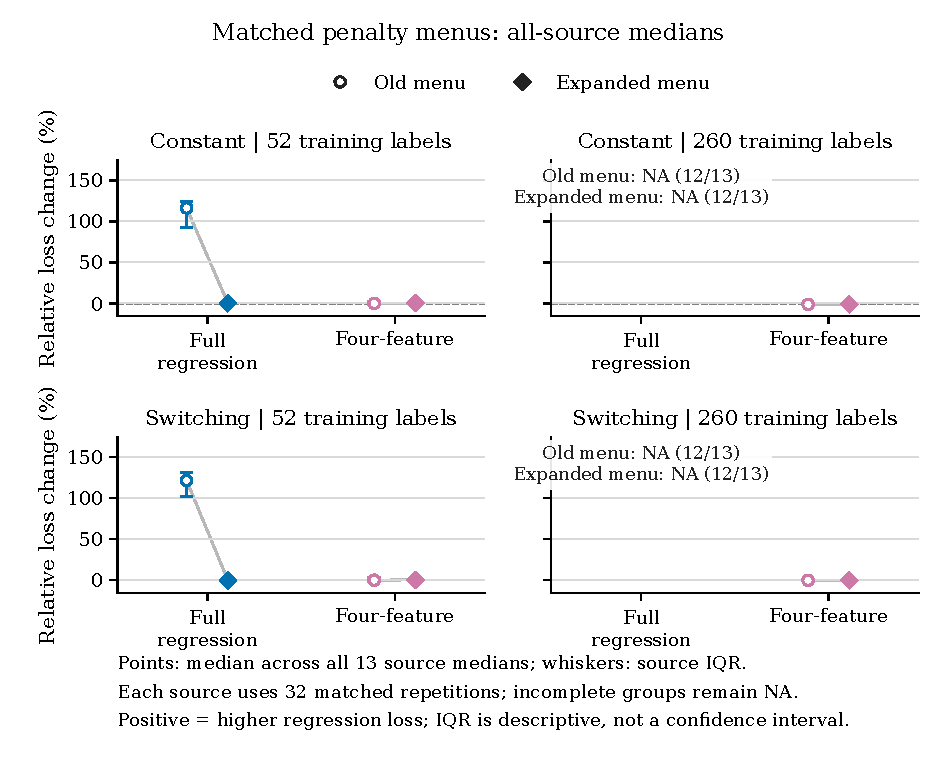
\includegraphics[width=.98\linewidth]{figures/v10-menu-isolation.pdf}
\caption{Paired penalty-menu isolation on unchanged calibrated paths. The expanded menu removes the large short-history full-regression loss in both arms. Longer-history full-regression summaries remain unavailable because a required repetition fails in each arm, with no successful-subset replacement.}\label{fig:mechanism}
\end{figure}

At history 260, one required full-regression repetition fails in each arm under the old low penalty. Both summaries across all thirteen sources remain unavailable. The experiment retains every failed cell and performs no retry. Earlier daily moment-qualification and hourly optimization failures also remain unavailable. Absence of a five-point switching increment is not evidence of equivalence.

The identification qualification above concerns the paired simulated menu intervention. The additional financial finite-menu diagnostic is described in Section~\ref{sup:v12-details}.

\paragraph{Procedure and complete-source inventory.}
Both QR variants use penalties $\{.001,.01,.1,1,10,\infty\}$; the infinite candidate is ordinary intercept-only I, distinct from corrected-rank F. Full regression requires every candidate to complete. Four-feature regression selects from its completed eligible candidates, as before. Exact ties now prefer stronger shrinkage in both variants; no actual exact tie occurred. The switching-phase denominator remains thirty-two. Two pilot repetitions selected the full thirty-two formal repetitions before launch. The simulated feature clock is inherited hourly geometry despite weekly calibration parameters; it is not a literal weekly-calendar replay.

The design preceded every new path calculation. M1 requires the constant-arm history-52 full-regression median within five percent of F. M2 requires the switching median at least five percentage points higher. M3 requires both aggregate improvements and at least twelve jointly improving sources. M1 and M3 hold; M2 fails. Full history-260 regression summaries remain unavailable after the required TIPS-G11 repetition fails in both arms. Successful repetitions or twelve-source subsets never replace them.

\par\smallskip\noindent\begin{minipage}{\linewidth}\footnotesize Constant=C; switching=S. Positive percentages mean higher loss than F. NA retains the whole failed cell; source medians and old results remain separate.\end{minipage}
Table~\ref{tab:v10-menu-full} retains the complete source, arm, history and method inventory.
\begingroup\scriptsize\renewcommand{\arraystretch}{.96}
\begin{longtable}{llrrrrrl}
\caption{Every menu-isolation source/arm/history/method cell. Relative-loss medians use all required repetitions.}\label{tab:v10-menu-full}\\
\toprule Source & Arm & History & Predictors & Original median & Expanded median & Complete/required & State \\\midrule\endfirsthead
\toprule Source & Arm & History & Predictors & Original median & Expanded median & Complete/required & State \\\midrule\endhead
GS-B & C & 52 & 33 & 117.16 & 4.24 & 32/32 & COMPLETE \\
GS-B & C & 52 & 4 & 7.20 & 8.70 & 32/32 & COMPLETE \\
GS-B & C & 260 & 33 & 2.90 & 0.10 & 32/32 & COMPLETE \\
GS-B & C & 260 & 4 & -2.02 & -1.92 & 32/32 & COMPLETE \\
GS-B & S & 52 & 33 & 91.35 & 2.47 & 32/32 & COMPLETE \\
GS-B & S & 52 & 4 & 3.22 & 3.17 & 32/32 & COMPLETE \\
GS-B & S & 260 & 33 & 4.56 & 0.56 & 32/32 & COMPLETE \\
GS-B & S & 260 & 4 & 0.23 & 0.09 & 32/32 & COMPLETE \\
MBS-TOT & C & 52 & 33 & 79.84 & -0.49 & 32/32 & COMPLETE \\
MBS-TOT & C & 52 & 4 & -0.87 & -0.70 & 32/32 & COMPLETE \\
MBS-TOT & C & 260 & 33 & 7.02 & 0.97 & 32/32 & COMPLETE \\
MBS-TOT & C & 260 & 4 & -5.00 & -5.15 & 32/32 & COMPLETE \\
MBS-TOT & S & 52 & 33 & 140.83 & -0.59 & 32/32 & COMPLETE \\
MBS-TOT & S & 52 & 4 & -0.44 & -0.92 & 32/32 & COMPLETE \\
MBS-TOT & S & 260 & 33 & 18.77 & 0.91 & 32/32 & COMPLETE \\
MBS-TOT & S & 260 & 4 & -0.06 & -0.22 & 32/32 & COMPLETE \\
CS-TOT & C & 52 & 33 & 124.34 & -3.01 & 32/32 & COMPLETE \\
CS-TOT & C & 52 & 4 & -3.07 & -3.07 & 32/32 & COMPLETE \\
CS-TOT & C & 260 & 33 & 2.68 & -0.19 & 32/32 & COMPLETE \\
CS-TOT & C & 260 & 4 & -1.21 & -1.13 & 32/32 & COMPLETE \\
CS-TOT & S & 52 & 33 & 124.34 & -3.01 & 32/32 & COMPLETE \\
CS-TOT & S & 52 & 4 & -3.07 & -3.07 & 32/32 & COMPLETE \\
CS-TOT & S & 260 & 33 & 2.68 & -0.19 & 32/32 & COMPLETE \\
CS-TOT & S & 260 & 4 & -1.21 & -1.13 & 32/32 & COMPLETE \\
FGS-TOT & C & 52 & 33 & 201.01 & 4.44 & 32/32 & COMPLETE \\
FGS-TOT & C & 52 & 4 & 1.90 & 1.90 & 32/32 & COMPLETE \\
FGS-TOT & C & 260 & 33 & 13.76 & 1.34 & 32/32 & COMPLETE \\
FGS-TOT & C & 260 & 4 & -2.98 & -2.98 & 32/32 & COMPLETE \\
FGS-TOT & S & 52 & 33 & 170.12 & -0.23 & 32/32 & COMPLETE \\
FGS-TOT & S & 52 & 4 & -4.36 & -4.36 & 32/32 & COMPLETE \\
FGS-TOT & S & 260 & 33 & 15.48 & -0.40 & 32/32 & COMPLETE \\
FGS-TOT & S & 260 & 4 & 0.23 & 0.48 & 32/32 & COMPLETE \\
TIPS-L2 & C & 52 & 33 & 119.29 & -0.54 & 32/32 & COMPLETE \\
TIPS-L2 & C & 52 & 4 & -2.10 & -2.10 & 32/32 & COMPLETE \\
TIPS-L2 & C & 260 & 33 & 9.32 & 0.64 & 32/32 & COMPLETE \\
TIPS-L2 & C & 260 & 4 & -1.69 & -1.69 & 32/32 & COMPLETE \\
TIPS-L2 & S & 52 & 33 & 101.92 & 0.53 & 32/32 & COMPLETE \\
TIPS-L2 & S & 52 & 4 & -0.03 & 0.38 & 32/32 & COMPLETE \\
TIPS-L2 & S & 260 & 33 & 8.88 & -0.38 & 32/32 & COMPLETE \\
TIPS-L2 & S & 260 & 4 & -0.27 & -0.28 & 32/32 & COMPLETE \\
TIPS-G11 & C & 52 & 33 & 131.26 & 0.98 & 32/32 & COMPLETE \\
TIPS-G11 & C & 52 & 4 & 1.11 & 1.14 & 32/32 & COMPLETE \\
TIPS-G11 & C & 260 & 33 & NA & NA & 31/32 & FAILED \\
TIPS-G11 & C & 260 & 4 & -0.48 & -0.49 & 32/32 & COMPLETE \\
TIPS-G11 & S & 52 & 33 & 131.26 & 0.98 & 32/32 & COMPLETE \\
TIPS-G11 & S & 52 & 4 & 1.11 & 1.14 & 32/32 & COMPLETE \\
TIPS-G11 & S & 260 & 33 & NA & NA & 31/32 & FAILED \\
TIPS-G11 & S & 260 & 4 & -0.48 & -0.49 & 32/32 & COMPLETE \\
TIPS-G2 & C & 52 & 33 & 107.85 & -4.00 & 32/32 & COMPLETE \\
TIPS-G2 & C & 52 & 4 & -1.55 & -1.69 & 32/32 & COMPLETE \\
TIPS-G2 & C & 260 & 33 & 13.09 & 0.12 & 32/32 & COMPLETE \\
TIPS-G2 & C & 260 & 4 & -0.29 & -0.43 & 32/32 & COMPLETE \\
TIPS-G2 & S & 52 & 33 & 107.85 & -4.00 & 32/32 & COMPLETE \\
TIPS-G2 & S & 52 & 4 & -1.55 & -1.69 & 32/32 & COMPLETE \\
TIPS-G2 & S & 260 & 33 & 13.09 & 0.12 & 32/32 & COMPLETE \\
TIPS-G2 & S & 260 & 4 & -0.29 & -0.43 & 32/32 & COMPLETE \\
TIPS-G6L11 & C & 52 & 33 & 92.36 & 1.00 & 32/32 & COMPLETE \\
TIPS-G6L11 & C & 52 & 4 & 0.11 & 0.44 & 32/32 & COMPLETE \\
TIPS-G6L11 & C & 260 & 33 & 15.63 & 2.53 & 32/32 & COMPLETE \\
TIPS-G6L11 & C & 260 & 4 & -0.54 & -0.64 & 32/32 & COMPLETE \\
TIPS-G6L11 & S & 52 & 33 & 121.40 & 3.18 & 32/32 & COMPLETE \\
TIPS-G6L11 & S & 52 & 4 & 3.27 & 3.68 & 32/32 & COMPLETE \\
TIPS-G6L11 & S & 260 & 33 & 20.88 & 1.90 & 32/32 & COMPLETE \\
TIPS-G6L11 & S & 260 & 4 & 1.23 & 1.23 & 32/32 & COMPLETE \\
GSC-L2 & C & 52 & 33 & 116.24 & 0.21 & 32/32 & COMPLETE \\
GSC-L2 & C & 52 & 4 & -0.02 & 1.85 & 32/32 & COMPLETE \\
GSC-L2 & C & 260 & 33 & 10.40 & -0.21 & 32/32 & COMPLETE \\
GSC-L2 & C & 260 & 4 & -0.80 & -1.22 & 32/32 & COMPLETE \\
GSC-L2 & S & 52 & 33 & 123.05 & -1.88 & 32/32 & COMPLETE \\
GSC-L2 & S & 52 & 4 & -2.47 & -2.17 & 32/32 & COMPLETE \\
GSC-L2 & S & 260 & 33 & 24.51 & 0.08 & 32/32 & COMPLETE \\
GSC-L2 & S & 260 & 4 & 0.81 & 0.87 & 32/32 & COMPLETE \\
GSC-G2L3 & C & 52 & 33 & 112.85 & 0.74 & 32/32 & COMPLETE \\
GSC-G2L3 & C & 52 & 4 & -0.43 & -0.28 & 32/32 & COMPLETE \\
GSC-G2L3 & C & 260 & 33 & 1.42 & 0.36 & 32/32 & COMPLETE \\
GSC-G2L3 & C & 260 & 4 & -1.39 & -1.02 & 32/32 & COMPLETE \\
GSC-G2L3 & S & 52 & 33 & 109.05 & 0.02 & 32/32 & COMPLETE \\
GSC-G2L3 & S & 52 & 4 & 10.61 & 10.73 & 32/32 & COMPLETE \\
GSC-G2L3 & S & 260 & 33 & -0.63 & -1.22 & 32/32 & COMPLETE \\
GSC-G2L3 & S & 260 & 4 & -3.84 & -3.95 & 32/32 & COMPLETE \\
GSC-G3L6 & C & 52 & 33 & 135.13 & 0.90 & 32/32 & COMPLETE \\
GSC-G3L6 & C & 52 & 4 & 2.78 & 2.43 & 32/32 & COMPLETE \\
GSC-G3L6 & C & 260 & 33 & -1.44 & -1.16 & 32/32 & COMPLETE \\
GSC-G3L6 & C & 260 & 4 & -1.26 & -1.37 & 32/32 & COMPLETE \\
GSC-G3L6 & S & 52 & 33 & 166.48 & 4.12 & 32/32 & COMPLETE \\
GSC-G3L6 & S & 52 & 4 & 5.26 & 6.42 & 32/32 & COMPLETE \\
GSC-G3L6 & S & 260 & 33 & 13.34 & 1.34 & 32/32 & COMPLETE \\
GSC-G3L6 & S & 260 & 4 & 0.31 & 0.61 & 32/32 & COMPLETE \\
GSC-G6L7 & C & 52 & 33 & 90.84 & -0.32 & 32/32 & COMPLETE \\
GSC-G6L7 & C & 52 & 4 & 1.73 & 2.14 & 32/32 & COMPLETE \\
GSC-G6L7 & C & 260 & 33 & 9.12 & 0.02 & 32/32 & COMPLETE \\
GSC-G6L7 & C & 260 & 4 & -0.66 & -0.75 & 32/32 & COMPLETE \\
GSC-G6L7 & S & 52 & 33 & 90.84 & -0.32 & 32/32 & COMPLETE \\
GSC-G6L7 & S & 52 & 4 & 1.73 & 2.14 & 32/32 & COMPLETE \\
GSC-G6L7 & S & 260 & 33 & 9.12 & 0.02 & 32/32 & COMPLETE \\
GSC-G6L7 & S & 260 & 4 & -0.66 & -0.75 & 32/32 & COMPLETE \\
GSC-G7L11 & C & 52 & 33 & 92.90 & -0.52 & 32/32 & COMPLETE \\
GSC-G7L11 & C & 52 & 4 & -4.71 & -4.35 & 32/32 & COMPLETE \\
GSC-G7L11 & C & 260 & 33 & 3.61 & -0.36 & 32/32 & COMPLETE \\
GSC-G7L11 & C & 260 & 4 & -0.51 & -0.55 & 32/32 & COMPLETE \\
GSC-G7L11 & S & 52 & 33 & 80.11 & -2.78 & 32/32 & COMPLETE \\
GSC-G7L11 & S & 52 & 4 & -2.03 & -2.67 & 32/32 & COMPLETE \\
GSC-G7L11 & S & 260 & 33 & -3.41 & 0.20 & 32/32 & COMPLETE \\
GSC-G7L11 & S & 260 & 4 & -5.15 & -5.15 & 32/32 & COMPLETE \\
\bottomrule\end{longtable}\endgroup


\clearpage
\section{CFTC sources, eligibility and information dates}\label{sup:v10-cftc}
The source is the CFTC TFF futures-only historical backcast for 2006--2016 plus annual 2017--2026 files. The retained observations begin in 2010. All eleven original source records remain public; no other new financial data were acquired.

A complete generated calendar contains 877 Monday-labeled report weeks, from 2010-01-04 through 2026-10-19. Economic position dates are retained separately. A code needs one valid observation per week, a stable exchange and stable contract units. Missing weeks, duplicates and changes disqualify a contract rather than trigger interpolation or splicing. Known consolidation prefixes 13874,20974,12460 are excluded before ranking. This conservative rule is broader than the documented plus-suffixed codes. Full-period mean open interest ranks survivors, with literal-code ties. Seventeen of 141 observed codes qualify; the top-twenty cap never changes that count.
The \href{https://github.com/ByronLi0207/financial-mathematics-paper-20261020/blob/revision-v10b/results/v10/cftc/eligibility.json}{complete code-level eligibility and exclusions} preserve every screening decision.

Validation indices are 553--604; evaluation indices are 611--870. All labels use horizon six, leaving six unissued origins between the segments. Validation position dates are 2020-08-11--2021-08-03; the last validation label ends 2021-09-14. Evaluation position dates are 2021-09-21--2026-09-08; the last evaluation label ends 2026-10-20. Training labels at refit r span r-H-W+1 through r-H. Monday labels index the inherited feature calendar; they do not claim Monday public availability. Actual positions are normally measured Tuesday and released Friday at 15:30 Eastern. Holiday, shutdown and ION-related publication delays prevent a first-release interpretation.

The selected category series are listed below. Net positions equal dealer long minus short in raw contract counts. Equal-weight median percentage changes preserve within-contract units; they are not common-dollar portfolio risk.
\begin{center}\scriptsize\begin{longtable}{lp{7.1cm}rr}
\toprule Code & Latest contract name & Mean open interest & Weeks \\\midrule\endhead
044601 & UST 5Y NOTE - CHICAGO BOARD OF TRADE & 3479174.2 & 877 \\
043602 & UST 10Y NOTE - CHICAGO BOARD OF TRADE & 3344673.4 & 877 \\
042601 & UST 2Y NOTE - CHICAGO BOARD OF TRADE & 2170647.9 & 877 \\
045601 & FED FUNDS - CHICAGO BOARD OF TRADE & 1282757.7 & 877 \\
020601 & UST BOND - CHICAGO BOARD OF TRADE & 999944.0 & 877 \\
099741 & EURO FX - CHICAGO MERCANTILE EXCHANGE & 503616.5 & 877 \\
1170E1 & VIX FUTURES - CBOE FUTURES EXCHANGE & 356897.7 & 877 \\
097741 & JAPANESE YEN - CHICAGO MERCANTILE EXCHANGE & 210863.1 & 877 \\
096742 & BRITISH POUND - CHICAGO MERCANTILE EXCHANGE & 197853.5 & 877 \\
095741 & MEXICAN PESO - CHICAGO MERCANTILE EXCHANGE & 174995.0 & 877 \\
090741 & CANADIAN DOLLAR - CHICAGO MERCANTILE EXCHANGE & 166229.3 & 877 \\
232741 & AUSTRALIAN DOLLAR - CHICAGO MERCANTILE EXCHANGE & 154802.4 & 877 \\
33874A & E-MINI S\&P 400 STOCK INDEX - CHICAGO MERCANTILE EXCHANGE & 75156.1 & 877 \\
240743 & NIKKEI STOCK AVERAGE YEN DENOM - CHICAGO MERCANTILE EXCHANGE & 59766.6 & 877 \\
092741 & SWISS FRANC - CHICAGO MERCANTILE EXCHANGE & 57197.3 & 877 \\
098662 & USD INDEX - ICE FUTURES U.S. & 52473.9 & 877 \\
112741 & NZ DOLLAR - CHICAGO MERCANTILE EXCHANGE & 44292.0 & 877 \\
\bottomrule\end{longtable}\end{center}

The six methods are corrected-rank F, ordinary I, four- and thirty-three-predictor regression, and finite delayed calibration of historical headroom and full regression. Both regressions use the six-point menu. The paired ACI wrappers retain the existing finite calibration with delayed matured feedback; no asymptotic coverage claim is attached. The complete 204 method cells finish without a numerical retry. The full cell CSV and trace ZIP retain absolute scores, breaches, selected penalties and gamma values.

For the CFTC delayed wrappers, gamma belongs to $\{.001,.005,.01,.05\}$. Completed candidates rank by validation coverage-distance, then pinball loss, then smaller gamma. Initialization requires at least nineteen matured scores. Updates wait for the full six-record label, and evaluation carries the validation state. The six unissued gap origins create no artificial reports or feedback events. These settings accompany histories 52/260, 52 validation origins, 260 evaluation origins and 13-record refits; none is retuned after evaluation.

Two narrow official-format clarifications follow the original design and acquisition but precede every forecast. The first accepts only the official midnight suffix after the date; the second accepts integer counts written with an all-zero decimal suffix. Neither changes a mathematical count, sample threshold, screen or forecast setting. Original failed technical preparation receipts remain visible. This is not a claim of fully observation-blind ingestion design.

\clearpage
\section{Complete model confidence sets}\label{sup:v10-mcs}
The pre-specified ninety-percent MCS uses the range statistic and 1,000 stationary-bootstrap draws, with block length $\max\{H,\lceil n^{1/3}\rceil\}$ in arch 8.0.0. Deterministic source/grid seeds and method order are recorded in the design. Every claimed complete report uses its entire declared origin grid and common target. Missing stored losses are derived only from saved reports, without issuing forecasts or fitting models. Every one of 98 comparisons completes. The 60 known unavailable slots remain unavailable, not statistical exclusions.

Distinct procedure labels retain their classification even when a selected penalty is infinite or reports coincide. Exact duplicate loss columns enter the library once; all associated procedure labels then receive the same p-value and inclusion partition. Conditional slots use their declared procedure identity. Matched F/I membership, literal uniqueness and unique-loss-class membership differ. Across the entire inventory, 90/98 sets contain matched F/I, 2/98 have a sole literal F/I member, and 4/98 have a sole loss class containing F/I. Conditional exclusion is 197/683 complete slots. Related sources and overlapping tasks provide no independent cross-grid test or simultaneous future guarantee.

Tables S36--S45 retain every source-specific membership result and method p-value, including unavailable procedures.
% Generated by notes/v10/build_mcs_compact.py; display only.
\begingroup
\fontsize{7.1}{8.5}\selectfont
\setlength{\tabcolsep}{1.35pt}
\renewcommand{\arraystretch}{1.06}
\setlength{\LTcapwidth}{\linewidth}
\noindent\textbf{Complete pre-specified MCS membership and p-values.}
All 98 source/period/$H$/$W$ comparisons are retained. Bold p-values denote included procedures using the saved literal rule $p>0.10$; ordinary type denotes exclusion. Values are rounded to three decimals only for display. Membership uses unrounded saved values; exact p-values are public in \texttt{results/v10/mcs/report-values.json}. \textsc{NA} denotes a known unavailable procedure, never a statistical exclusion; --- means that procedure was not pre-specified in that particular grid.
Multi-member exact-loss classes carry a superscript equal to the representative method ID on \emph{every} member, including the representative. Unmarked values are singleton classes. Method IDs are display aliases only; all full labels and classifications appear in the final legend.
The pre-specified procedure uses 1000 stationary-bootstrap replications, confidence 0.90, statistic $R$, and block length $\max\{H,\lceil n^{1/3}\rceil\}$. Analytic identical-loss or single-method cases retain their saved status; no new inference is performed for this table.

\noindent\textbf{FX original.} Each method column is shown once for every row of this group.\par
\begin{longtable}{@{}lrrrrrrrrrrrrrr@{}}
\caption{FX original; method block 1/3. Full-grid $n=6625$.}\\
\toprule
Source & \rotatebox{90}{Horizon} & \rotatebox{90}{History} & \rotatebox{90}{\shortstack[l]{Hist.\\headroom}} & \rotatebox{90}{\shortstack[l]{Intercept\\only}} & \rotatebox{90}{\shortstack[l]{Cal. SAV\\history}} & \rotatebox{90}{\shortstack[l]{Cal. SAV\\regression}} & \rotatebox{90}{\shortstack[l]{SAV\\headroom}} & \rotatebox{90}{\shortstack[l]{Expanded\\full reg.}} & \rotatebox{90}{\shortstack[l]{Endpoint\\plug-in}} & \rotatebox{90}{\shortstack[l]{Four-\\feature}} & \rotatebox{90}{\shortstack[l]{Legacy\\multi-fold}} & \rotatebox{90}{\shortstack[l]{Finite\\ridge}} & \rotatebox{90}{\shortstack[l]{Expanded\\ridge}} & \rotatebox{90}{\shortstack[l]{One-SE\\ridge}} \\
\midrule
\endfirsthead
\toprule
Source & \rotatebox{90}{Horizon} & \rotatebox{90}{History} & \rotatebox{90}{\shortstack[l]{Hist.\\headroom}} & \rotatebox{90}{\shortstack[l]{Intercept\\only}} & \rotatebox{90}{\shortstack[l]{Cal. SAV\\history}} & \rotatebox{90}{\shortstack[l]{Cal. SAV\\regression}} & \rotatebox{90}{\shortstack[l]{SAV\\headroom}} & \rotatebox{90}{\shortstack[l]{Expanded\\full reg.}} & \rotatebox{90}{\shortstack[l]{Endpoint\\plug-in}} & \rotatebox{90}{\shortstack[l]{Four-\\feature}} & \rotatebox{90}{\shortstack[l]{Legacy\\multi-fold}} & \rotatebox{90}{\shortstack[l]{Finite\\ridge}} & \rotatebox{90}{\shortstack[l]{Expanded\\ridge}} & \rotatebox{90}{\shortstack[l]{One-SE\\ridge}} \\
\midrule
\endhead
\midrule\multicolumn{15}{r}{Continued on next page}\\\endfoot
\bottomrule\endlastfoot
fx\_hourly & 6 & 720 & $0.000$ & $0.002^{\mathrm{M02}}$ & $0.000$ & $0.019$ & $0.000$ & $0.040^{\mathrm{M10}}$ & $0.000$ & $0.010$ & \textsc{NA} & $0.040^{\mathrm{M10}}$ & $0.040^{\mathrm{M10}}$ & $0.002^{\mathrm{M02}}$ \\
fx\_hourly & 6 & 2880 & $0.000$ & $0.000^{\mathrm{M02}}$ & $0.000$ & $\mathbf{0.385}$ & $0.000$ & $\mathbf{1.000}^{\mathrm{M10}}$ & $0.000$ & $0.001$ & --- & $\mathbf{1.000}^{\mathrm{M10}}$ & $\mathbf{1.000}^{\mathrm{M10}}$ & $0.000^{\mathrm{M02}}$ \\
fx\_hourly & 24 & 720 & $\mathbf{0.696}$ & $\mathbf{0.760}\hphantom{^{\mathrm{M00}}}$ & $0.009$ & $0.000$ & $\mathbf{0.792}$ & $0.009^{\mathrm{M10}}$ & $0.011$ & $\mathbf{0.250}$ & \textsc{NA} & $0.009^{\mathrm{M10}}$ & $0.009^{\mathrm{M10}}$ & $0.009^{\mathrm{M10}}$ \\
fx\_hourly & 24 & 2880 & $\mathbf{0.360}$ & $\mathbf{0.360}\hphantom{^{\mathrm{M00}}}$ & $\mathbf{0.360}$ & $\mathbf{0.360}$ & $\mathbf{0.360}$ & $\mathbf{0.360}^{\mathrm{M10}}$ & $0.005$ & $\mathbf{0.360}$ & --- & $\mathbf{0.360}^{\mathrm{M10}}$ & $\mathbf{0.360}^{\mathrm{M10}}$ & $0.078^{\mathrm{M16}}$ \\
\end{longtable}

\begin{longtable}{@{}lrrrrrrrrrrrrrr@{}}
\caption{FX original; method block 2/3. Full-grid $n=6625$.}\\
\toprule
Source & \rotatebox{90}{Horizon} & \rotatebox{90}{History} & \rotatebox{90}{\shortstack[l]{Multi-fold\\one-SE}} & \rotatebox{90}{\shortstack[l]{Filtered\\paths}} & \rotatebox{90}{\shortstack[l]{Peak-tail\\fit}} & \rotatebox{90}{\shortstack[l]{Quantile\\forest}} & \rotatebox{90}{\shortstack[l]{Nearest\\states}} & \rotatebox{90}{\shortstack[l]{Original\\full reg.}} & \rotatebox{90}{\shortstack[l]{Scaled\\neighbors}} & \rotatebox{90}{\shortstack[l]{Fixed\\peak}} & \rotatebox{90}{\shortstack[l]{Fixed\\transl.}} & \rotatebox{90}{\shortstack[l]{State\\headroom}} & \rotatebox{90}{\shortstack[l]{State\\peak}} & \rotatebox{90}{\shortstack[l]{State\\transl.}} \\
\midrule
\endfirsthead
\toprule
Source & \rotatebox{90}{Horizon} & \rotatebox{90}{History} & \rotatebox{90}{\shortstack[l]{Multi-fold\\one-SE}} & \rotatebox{90}{\shortstack[l]{Filtered\\paths}} & \rotatebox{90}{\shortstack[l]{Peak-tail\\fit}} & \rotatebox{90}{\shortstack[l]{Quantile\\forest}} & \rotatebox{90}{\shortstack[l]{Nearest\\states}} & \rotatebox{90}{\shortstack[l]{Original\\full reg.}} & \rotatebox{90}{\shortstack[l]{Scaled\\neighbors}} & \rotatebox{90}{\shortstack[l]{Fixed\\peak}} & \rotatebox{90}{\shortstack[l]{Fixed\\transl.}} & \rotatebox{90}{\shortstack[l]{State\\headroom}} & \rotatebox{90}{\shortstack[l]{State\\peak}} & \rotatebox{90}{\shortstack[l]{State\\transl.}} \\
\midrule
\endhead
\midrule\multicolumn{15}{r}{Continued on next page}\\\endfoot
\bottomrule\endlastfoot
fx\_hourly & 6 & 720 & --- & \textsc{NA} & \textsc{NA} & $0.002$ & $0.014$ & $0.040^{\mathrm{M10}}$ & $0.016$ & $0.000$ & $0.004$ & $0.002$ & $0.000$ & $0.014$ \\
fx\_hourly & 6 & 2880 & $\mathbf{1.000}^{\mathrm{M10}}$ & $0.000$ & $0.000$ & $0.001$ & $0.054$ & $\mathbf{1.000}^{\mathrm{M10}}$ & $0.039$ & $0.000$ & $0.000$ & --- & --- & --- \\
fx\_hourly & 24 & 720 & --- & \textsc{NA} & \textsc{NA} & $\mathbf{0.199}$ & $\mathbf{0.445}$ & $0.009^{\mathrm{M10}}$ & $\mathbf{0.347}$ & $0.000$ & $\mathbf{0.696}$ & $\mathbf{0.792}$ & $0.067$ & $\mathbf{0.792}$ \\
fx\_hourly & 24 & 2880 & $0.078^{\mathrm{M16}}$ & $0.079$ & $0.002$ & $\mathbf{0.153}$ & $0.078$ & $\mathbf{0.360}^{\mathrm{M10}}$ & $0.052$ & $0.000$ & $\mathbf{0.360}$ & --- & --- & --- \\
\end{longtable}

\begin{longtable}{@{}lrrrrrrr@{}}
\caption{FX original; method block 3/3. Full-grid $n=6625$.}\\
\toprule
Source & \rotatebox{90}{Horizon} & \rotatebox{90}{History} & \rotatebox{90}{\shortstack[l]{Rolling\\headroom}} & \rotatebox{90}{\shortstack[l]{Rolling\\peak}} & \rotatebox{90}{\shortstack[l]{Rolling\\transl.}} & \rotatebox{90}{\shortstack[l]{Mean\\combination}} & \rotatebox{90}{\shortstack[l]{Median\\combination}} \\
\midrule
\endfirsthead
\toprule
Source & \rotatebox{90}{Horizon} & \rotatebox{90}{History} & \rotatebox{90}{\shortstack[l]{Rolling\\headroom}} & \rotatebox{90}{\shortstack[l]{Rolling\\peak}} & \rotatebox{90}{\shortstack[l]{Rolling\\transl.}} & \rotatebox{90}{\shortstack[l]{Mean\\combination}} & \rotatebox{90}{\shortstack[l]{Median\\combination}} \\
\midrule
\endhead
\midrule\multicolumn{8}{r}{Continued on next page}\\\endfoot
\bottomrule\endlastfoot
fx\_hourly & 6 & 720 & $0.002$ & $0.000$ & $0.003$ & $\mathbf{1.000}$ & $0.047$ \\
fx\_hourly & 6 & 2880 & $0.000$ & $0.000$ & $0.000$ & $0.039$ & $0.057$ \\
fx\_hourly & 24 & 720 & $\mathbf{0.792}$ & $0.000$ & $\mathbf{1.000}$ & $\mathbf{0.696}$ & $\mathbf{0.551}$ \\
fx\_hourly & 24 & 2880 & $\mathbf{0.360}$ & $0.000$ & $\mathbf{0.360}$ & $\mathbf{1.000}$ & $\mathbf{0.360}$ \\
\end{longtable}

\clearpage
\noindent\textbf{FX early 2015.} Each method column is shown once for every row of this group.\par
\begin{longtable}{@{}lrrrrrrrrrrr@{}}
\caption{FX early 2015; method block 1/1. Full-grid $n=1440$.}\\
\toprule
Source & \rotatebox{90}{Horizon} & \rotatebox{90}{History} & \rotatebox{90}{\shortstack[l]{Hist.\\headroom}} & \rotatebox{90}{\shortstack[l]{Intercept\\only}} & \rotatebox{90}{\shortstack[l]{Legacy\\multi-fold}} & \rotatebox{90}{\shortstack[l]{Finite\\ridge}} & \rotatebox{90}{\shortstack[l]{Expanded\\ridge}} & \rotatebox{90}{\shortstack[l]{One-SE\\ridge}} & \rotatebox{90}{\shortstack[l]{Multi-fold\\one-SE}} & \rotatebox{90}{\shortstack[l]{Original\\full reg.}} & \rotatebox{90}{\shortstack[l]{Original\\roll. hist.}} \\
\midrule
\endfirsthead
\toprule
Source & \rotatebox{90}{Horizon} & \rotatebox{90}{History} & \rotatebox{90}{\shortstack[l]{Hist.\\headroom}} & \rotatebox{90}{\shortstack[l]{Intercept\\only}} & \rotatebox{90}{\shortstack[l]{Legacy\\multi-fold}} & \rotatebox{90}{\shortstack[l]{Finite\\ridge}} & \rotatebox{90}{\shortstack[l]{Expanded\\ridge}} & \rotatebox{90}{\shortstack[l]{One-SE\\ridge}} & \rotatebox{90}{\shortstack[l]{Multi-fold\\one-SE}} & \rotatebox{90}{\shortstack[l]{Original\\full reg.}} & \rotatebox{90}{\shortstack[l]{Original\\roll. hist.}} \\
\midrule
\endhead
\midrule\multicolumn{12}{r}{Continued on next page}\\\endfoot
\bottomrule\endlastfoot
fx\_hourly & 6 & 720 & $0.063$ & $\mathbf{0.675}$ & \textsc{NA} & $\mathbf{0.675}^{\mathrm{M14}}$ & $\mathbf{0.675}^{\mathrm{M14}}$ & $\mathbf{0.628}\hphantom{^{\mathrm{M00}}}$ & --- & --- & $\mathbf{1.000}$ \\
fx\_hourly & 6 & 2880 & $0.000$ & $0.000$ & --- & $\mathbf{1.000}^{\mathrm{M14}}$ & $\mathbf{1.000}^{\mathrm{M14}}$ & $0.009\hphantom{^{\mathrm{M00}}}$ & $\mathbf{1.000}^{\mathrm{M14}}$ & $\mathbf{1.000}^{\mathrm{M14}}$ & --- \\
fx\_hourly & 24 & 720 & $0.014$ & $\mathbf{0.242}$ & \textsc{NA} & $\mathbf{1.000}^{\mathrm{M14}}$ & $\mathbf{1.000}^{\mathrm{M14}}$ & $\mathbf{1.000}^{\mathrm{M14}}$ & --- & --- & --- \\
fx\_hourly & 24 & 2880 & $0.000$ & $\mathbf{0.910}$ & --- & $\mathbf{1.000}^{\mathrm{M14}}$ & $\mathbf{1.000}^{\mathrm{M14}}$ & $\mathbf{0.991}^{\mathrm{M16}}$ & $\mathbf{0.991}^{\mathrm{M16}}$ & --- & --- \\
\end{longtable}

\clearpage
\noindent\textbf{Treasury bills.} Each method column is shown once for every row of this group.\par
\begin{longtable}{@{}lrrrrrrrrrrrrrr@{}}
\caption{Treasury bills; method block 1/3. Full-grid $n=277$.}\\
\toprule
Source & \rotatebox{90}{Horizon} & \rotatebox{90}{History} & \rotatebox{90}{\shortstack[l]{Hist.\\headroom}} & \rotatebox{90}{\shortstack[l]{Intercept\\only}} & \rotatebox{90}{\shortstack[l]{Cal. SAV\\history}} & \rotatebox{90}{\shortstack[l]{Cal. SAV\\regression}} & \rotatebox{90}{\shortstack[l]{SAV\\headroom}} & \rotatebox{90}{\shortstack[l]{Expanded\\full reg.}} & \rotatebox{90}{\shortstack[l]{Endpoint\\plug-in}} & \rotatebox{90}{\shortstack[l]{Four-\\feature}} & \rotatebox{90}{\shortstack[l]{Finite\\ridge}} & \rotatebox{90}{\shortstack[l]{Expanded\\ridge}} & \rotatebox{90}{\shortstack[l]{One-SE\\ridge}} & \rotatebox{90}{\shortstack[l]{Multi-fold\\one-SE}} \\
\midrule
\endfirsthead
\toprule
Source & \rotatebox{90}{Horizon} & \rotatebox{90}{History} & \rotatebox{90}{\shortstack[l]{Hist.\\headroom}} & \rotatebox{90}{\shortstack[l]{Intercept\\only}} & \rotatebox{90}{\shortstack[l]{Cal. SAV\\history}} & \rotatebox{90}{\shortstack[l]{Cal. SAV\\regression}} & \rotatebox{90}{\shortstack[l]{SAV\\headroom}} & \rotatebox{90}{\shortstack[l]{Expanded\\full reg.}} & \rotatebox{90}{\shortstack[l]{Endpoint\\plug-in}} & \rotatebox{90}{\shortstack[l]{Four-\\feature}} & \rotatebox{90}{\shortstack[l]{Finite\\ridge}} & \rotatebox{90}{\shortstack[l]{Expanded\\ridge}} & \rotatebox{90}{\shortstack[l]{One-SE\\ridge}} & \rotatebox{90}{\shortstack[l]{Multi-fold\\one-SE}} \\
\midrule
\endhead
\midrule\multicolumn{15}{r}{Continued on next page}\\\endfoot
\bottomrule\endlastfoot
nyfed\_weekly & 6 & 52 & $\mathbf{0.809}^{\mathrm{M01}}$ & $\mathbf{0.400}^{\mathrm{M02}}$ & $0.000$ & $0.004$ & $0.045$ & $\mathbf{0.940}^{\mathrm{M10}}$ & $\mathbf{0.810}$ & $\mathbf{0.770}$ & $\mathbf{0.940}^{\mathrm{M10}}$ & $\mathbf{0.400}^{\mathrm{M02}}$ & $\mathbf{0.400}^{\mathrm{M02}}$ & $\mathbf{0.400}^{\mathrm{M02}}$ \\
nyfed\_weekly & 6 & 260 & $\mathbf{0.663}\hphantom{^{\mathrm{M00}}}$ & $0.073\hphantom{^{\mathrm{M00}}}$ & $\mathbf{0.144}$ & $\mathbf{0.194}$ & $\mathbf{0.273}$ & $\mathbf{0.452}^{\mathrm{M10}}$ & $\mathbf{0.982}$ & $\mathbf{0.622}$ & $\mathbf{0.452}^{\mathrm{M10}}$ & $\mathbf{0.452}^{\mathrm{M10}}$ & $\mathbf{0.622}^{\mathrm{M16}}$ & $\mathbf{0.622}^{\mathrm{M16}}$ \\
nyfed\_weekly & 24 & 52 & $\mathbf{0.862}^{\mathrm{M01}}$ & $\mathbf{0.626}^{\mathrm{M02}}$ & $\mathbf{0.926}$ & $0.004$ & $\mathbf{0.253}$ & $\mathbf{0.925}^{\mathrm{M10}}$ & $\mathbf{0.211}$ & $\mathbf{0.150}$ & $\mathbf{0.925}^{\mathrm{M10}}$ & $\mathbf{0.626}^{\mathrm{M02}}$ & $\mathbf{0.626}^{\mathrm{M02}}$ & $\mathbf{0.626}^{\mathrm{M02}}$ \\
nyfed\_weekly & 24 & 260 & $0.066\hphantom{^{\mathrm{M00}}}$ & $\mathbf{0.165}^{\mathrm{M02}}$ & \textsc{NA} & \textsc{NA} & $\mathbf{0.261}$ & $\mathbf{0.186}^{\mathrm{M10}}$ & $\mathbf{0.186}$ & $\mathbf{0.178}$ & $\mathbf{0.186}^{\mathrm{M10}}$ & $\mathbf{0.186}^{\mathrm{M10}}$ & $\mathbf{0.165}^{\mathrm{M02}}$ & $\mathbf{0.165}^{\mathrm{M02}}$ \\
\end{longtable}

\begin{longtable}{@{}lrrrrrrrrrrrrrr@{}}
\caption{Treasury bills; method block 2/3. Full-grid $n=277$.}\\
\toprule
Source & \rotatebox{90}{Horizon} & \rotatebox{90}{History} & \rotatebox{90}{\shortstack[l]{Filtered\\paths}} & \rotatebox{90}{\shortstack[l]{Peak-tail\\fit}} & \rotatebox{90}{\shortstack[l]{Quantile\\forest}} & \rotatebox{90}{\shortstack[l]{Nearest\\states}} & \rotatebox{90}{\shortstack[l]{Original\\full reg.}} & \rotatebox{90}{\shortstack[l]{Scaled\\neighbors}} & \rotatebox{90}{\shortstack[l]{Fixed\\peak}} & \rotatebox{90}{\shortstack[l]{Fixed\\transl.}} & \rotatebox{90}{\shortstack[l]{State\\headroom}} & \rotatebox{90}{\shortstack[l]{State\\peak}} & \rotatebox{90}{\shortstack[l]{State\\transl.}} & \rotatebox{90}{\shortstack[l]{Rolling\\headroom}} \\
\midrule
\endfirsthead
\toprule
Source & \rotatebox{90}{Horizon} & \rotatebox{90}{History} & \rotatebox{90}{\shortstack[l]{Filtered\\paths}} & \rotatebox{90}{\shortstack[l]{Peak-tail\\fit}} & \rotatebox{90}{\shortstack[l]{Quantile\\forest}} & \rotatebox{90}{\shortstack[l]{Nearest\\states}} & \rotatebox{90}{\shortstack[l]{Original\\full reg.}} & \rotatebox{90}{\shortstack[l]{Scaled\\neighbors}} & \rotatebox{90}{\shortstack[l]{Fixed\\peak}} & \rotatebox{90}{\shortstack[l]{Fixed\\transl.}} & \rotatebox{90}{\shortstack[l]{State\\headroom}} & \rotatebox{90}{\shortstack[l]{State\\peak}} & \rotatebox{90}{\shortstack[l]{State\\transl.}} & \rotatebox{90}{\shortstack[l]{Rolling\\headroom}} \\
\midrule
\endhead
\midrule\multicolumn{15}{r}{Continued on next page}\\\endfoot
\bottomrule\endlastfoot
nyfed\_weekly & 6 & 52 & $\mathbf{0.940}$ & \textsc{NA} & $\mathbf{0.940}$ & $\mathbf{0.809}^{\mathrm{M01}}$ & $0.012$ & $0.016$ & $\mathbf{0.743}$ & $\mathbf{0.767}$ & $\mathbf{0.863}$ & $\mathbf{0.940}$ & $\mathbf{0.802}$ & $\mathbf{0.597}$ \\
nyfed\_weekly & 6 & 260 & $\mathbf{0.897}$ & $\mathbf{0.982}$ & $\mathbf{0.622}$ & $\mathbf{0.845}\hphantom{^{\mathrm{M00}}}$ & $0.028$ & $\mathbf{0.157}$ & $\mathbf{0.982}$ & $\mathbf{0.687}$ & $\mathbf{0.957}$ & $\mathbf{0.982}$ & $\mathbf{0.913}$ & $\mathbf{0.633}$ \\
nyfed\_weekly & 24 & 52 & $\mathbf{0.150}$ & \textsc{NA} & $\mathbf{0.977}$ & $\mathbf{0.862}^{\mathrm{M01}}$ & $\mathbf{0.211}$ & $0.025$ & $\mathbf{0.925}$ & $\mathbf{0.979}$ & $\mathbf{0.862}$ & $\mathbf{0.926}$ & $\mathbf{0.977}$ & $\mathbf{0.925}$ \\
nyfed\_weekly & 24 & 260 & $0.000$ & $0.000$ & $0.066$ & $\mathbf{0.261}\hphantom{^{\mathrm{M00}}}$ & $\mathbf{0.201}$ & $0.000$ & $\mathbf{0.487}$ & $0.072$ & $\mathbf{1.000}$ & $\mathbf{0.336}$ & $\mathbf{0.487}$ & $0.066$ \\
\end{longtable}

\begin{longtable}{@{}lrrrrrr@{}}
\caption{Treasury bills; method block 3/3. Full-grid $n=277$.}\\
\toprule
Source & \rotatebox{90}{Horizon} & \rotatebox{90}{History} & \rotatebox{90}{\shortstack[l]{Rolling\\peak}} & \rotatebox{90}{\shortstack[l]{Rolling\\transl.}} & \rotatebox{90}{\shortstack[l]{Mean\\combination}} & \rotatebox{90}{\shortstack[l]{Median\\combination}} \\
\midrule
\endfirsthead
\toprule
Source & \rotatebox{90}{Horizon} & \rotatebox{90}{History} & \rotatebox{90}{\shortstack[l]{Rolling\\peak}} & \rotatebox{90}{\shortstack[l]{Rolling\\transl.}} & \rotatebox{90}{\shortstack[l]{Mean\\combination}} & \rotatebox{90}{\shortstack[l]{Median\\combination}} \\
\midrule
\endhead
\midrule\multicolumn{7}{r}{Continued on next page}\\\endfoot
\bottomrule\endlastfoot
nyfed\_weekly & 6 & 52 & $\mathbf{1.000}$ & $\mathbf{0.516}$ & $\mathbf{0.940}$ & $\mathbf{0.809}^{\mathrm{M01}}$ \\
nyfed\_weekly & 6 & 260 & $\mathbf{1.000}$ & $\mathbf{0.663}$ & $\mathbf{0.622}$ & $\mathbf{0.848}\hphantom{^{\mathrm{M00}}}$ \\
nyfed\_weekly & 24 & 52 & $\mathbf{0.926}$ & $\mathbf{1.000}$ & $\mathbf{0.925}$ & $\mathbf{0.862}^{\mathrm{M01}}$ \\
nyfed\_weekly & 24 & 260 & $\mathbf{0.624}$ & $0.066$ & $\mathbf{0.336}$ & $\mathbf{0.321}\hphantom{^{\mathrm{M00}}}$ \\
\end{longtable}

\clearpage
\noindent\textbf{Other NYFed panels.} Each method column is shown once for every row of this group.\par
\begin{longtable}{@{}lrrrrrrrrrrrrrr@{}}
\caption{Other NYFed panels; method block 1/1. Full-grid $n=277$.}\\
\toprule
Source & \rotatebox{90}{Horizon} & \rotatebox{90}{History} & \rotatebox{90}{\shortstack[l]{Hist.\\headroom}} & \rotatebox{90}{\shortstack[l]{Intercept\\only}} & \rotatebox{90}{\shortstack[l]{Finite\\ridge}} & \rotatebox{90}{\shortstack[l]{Expanded\\ridge}} & \rotatebox{90}{\shortstack[l]{One-SE\\ridge}} & \rotatebox{90}{\shortstack[l]{Multi-fold\\one-SE}} & \rotatebox{90}{\shortstack[l]{Expanded\\full reg.}} & \rotatebox{90}{\shortstack[l]{Four-\\feature}} & \rotatebox{90}{\shortstack[l]{Endpoint\\plug-in}} & \rotatebox{90}{\shortstack[l]{Original\\full reg.}} & \rotatebox{90}{\shortstack[l]{Mean\\combination}} & \rotatebox{90}{\shortstack[l]{Median\\combination}} \\
\midrule
\endfirsthead
\toprule
Source & \rotatebox{90}{Horizon} & \rotatebox{90}{History} & \rotatebox{90}{\shortstack[l]{Hist.\\headroom}} & \rotatebox{90}{\shortstack[l]{Intercept\\only}} & \rotatebox{90}{\shortstack[l]{Finite\\ridge}} & \rotatebox{90}{\shortstack[l]{Expanded\\ridge}} & \rotatebox{90}{\shortstack[l]{One-SE\\ridge}} & \rotatebox{90}{\shortstack[l]{Multi-fold\\one-SE}} & \rotatebox{90}{\shortstack[l]{Expanded\\full reg.}} & \rotatebox{90}{\shortstack[l]{Four-\\feature}} & \rotatebox{90}{\shortstack[l]{Endpoint\\plug-in}} & \rotatebox{90}{\shortstack[l]{Original\\full reg.}} & \rotatebox{90}{\shortstack[l]{Mean\\combination}} & \rotatebox{90}{\shortstack[l]{Median\\combination}} \\
\midrule
\endhead
\midrule\multicolumn{15}{r}{Continued on next page}\\\endfoot
\bottomrule\endlastfoot
PDPOSCS-TOT & 6 & 52 & $\mathbf{0.312}$ & $\mathbf{1.000}^{\mathrm{M02}}$ & $\mathbf{0.312}^{\mathrm{M14}}$ & $\mathbf{1.000}^{\mathrm{M02}}$ & $\mathbf{1.000}^{\mathrm{M02}}$ & $\mathbf{1.000}^{\mathrm{M02}}$ & $\mathbf{0.312}^{\mathrm{M14}}$ & $\mathbf{0.312}$ & $\mathbf{0.172}$ & $0.095\hphantom{^{\mathrm{M00}}}$ & $\mathbf{0.312}$ & \textsc{NA} \\
PDPOSCS-TOT & 6 & 260 & $\mathbf{0.582}$ & $\mathbf{0.780}^{\mathrm{M02}}$ & $\mathbf{0.243}^{\mathrm{M14}}$ & $\mathbf{0.243}^{\mathrm{M14}}$ & $\mathbf{0.780}^{\mathrm{M02}}$ & $\mathbf{0.780}^{\mathrm{M02}}$ & $\mathbf{0.243}^{\mathrm{M14}}$ & $\mathbf{0.780}$ & $0.000$ & $\mathbf{0.697}\hphantom{^{\mathrm{M00}}}$ & $\mathbf{1.000}$ & \textsc{NA} \\
PDPOSCS-TOT & 24 & 52 & $\mathbf{0.898}$ & $\mathbf{0.898}^{\mathrm{M02}}$ & $\mathbf{0.780}^{\mathrm{M14}}$ & $\mathbf{0.898}^{\mathrm{M02}}$ & $\mathbf{0.898}^{\mathrm{M02}}$ & $\mathbf{0.898}^{\mathrm{M02}}$ & $\mathbf{0.780}^{\mathrm{M14}}$ & $\mathbf{0.898}$ & $\mathbf{1.000}$ & $0.085\hphantom{^{\mathrm{M00}}}$ & $\mathbf{0.780}$ & \textsc{NA} \\
PDPOSCS-TOT & 24 & 260 & $0.000$ & $\mathbf{1.000}^{\mathrm{M02}}$ & $0.010^{\mathrm{M14}}$ & $\mathbf{1.000}^{\mathrm{M02}}$ & $\mathbf{1.000}^{\mathrm{M02}}$ & $\mathbf{1.000}^{\mathrm{M02}}$ & $0.010^{\mathrm{M14}}$ & $0.000$ & $0.000$ & $0.003\hphantom{^{\mathrm{M00}}}$ & $0.000$ & \textsc{NA} \\
PDPOSFGS-TOT & 6 & 52 & $\mathbf{0.248}$ & $\mathbf{1.000}^{\mathrm{M02}}$ & $\mathbf{0.868}^{\mathrm{M14}}$ & $\mathbf{1.000}^{\mathrm{M02}}$ & $\mathbf{1.000}^{\mathrm{M02}}$ & $\mathbf{1.000}^{\mathrm{M02}}$ & $\mathbf{0.868}^{\mathrm{M14}}$ & $\mathbf{0.968}$ & $\mathbf{0.974}$ & $0.014\hphantom{^{\mathrm{M00}}}$ & $\mathbf{0.492}$ & \textsc{NA} \\
PDPOSFGS-TOT & 6 & 260 & $0.017$ & $0.039\hphantom{^{\mathrm{M00}}}$ & $\mathbf{1.000}^{\mathrm{M14}}$ & $\mathbf{1.000}^{\mathrm{M14}}$ & $\mathbf{1.000}^{\mathrm{M14}}$ & $\mathbf{1.000}^{\mathrm{M14}}$ & $\mathbf{1.000}^{\mathrm{M14}}$ & $0.001$ & $0.000$ & $\mathbf{0.709}\hphantom{^{\mathrm{M00}}}$ & $\mathbf{0.709}$ & \textsc{NA} \\
PDPOSFGS-TOT & 24 & 52 & $\mathbf{0.521}$ & $\mathbf{0.390}^{\mathrm{M02}}$ & $\mathbf{0.307}^{\mathrm{M14}}$ & $\mathbf{0.307}^{\mathrm{M14}}$ & $\mathbf{0.390}^{\mathrm{M02}}$ & $\mathbf{0.390}^{\mathrm{M02}}$ & $\mathbf{0.307}^{\mathrm{M14}}$ & $\mathbf{0.521}$ & $\mathbf{1.000}$ & $\mathbf{0.133}\hphantom{^{\mathrm{M00}}}$ & $\mathbf{0.390}$ & \textsc{NA} \\
PDPOSFGS-TOT & 24 & 260 & $0.010$ & $\mathbf{0.772}\hphantom{^{\mathrm{M00}}}$ & $\mathbf{0.772}^{\mathrm{M14}}$ & $\mathbf{0.772}^{\mathrm{M14}}$ & $\mathbf{0.772}^{\mathrm{M14}}$ & $\mathbf{0.772}^{\mathrm{M14}}$ & $\mathbf{0.772}^{\mathrm{M14}}$ & $0.000$ & $\mathbf{1.000}$ & $\mathbf{0.470}\hphantom{^{\mathrm{M00}}}$ & $\mathbf{0.425}$ & \textsc{NA} \\
PDPOSGSC-G2L3 & 6 & 52 & $\mathbf{1.000}$ & $\mathbf{0.208}\hphantom{^{\mathrm{M00}}}$ & $\mathbf{0.189}^{\mathrm{M14}}$ & $\mathbf{0.189}^{\mathrm{M14}}$ & $\mathbf{0.189}^{\mathrm{M14}}$ & $\mathbf{0.189}^{\mathrm{M14}}$ & $\mathbf{0.189}^{\mathrm{M14}}$ & $0.019$ & $0.035$ & $0.018\hphantom{^{\mathrm{M00}}}$ & $\mathbf{0.189}$ & \textsc{NA} \\
PDPOSGSC-G2L3 & 6 & 260 & $\mathbf{0.676}$ & $\mathbf{0.676}\hphantom{^{\mathrm{M00}}}$ & $\mathbf{0.118}^{\mathrm{M14}}$ & $\mathbf{0.118}^{\mathrm{M14}}$ & $\mathbf{0.676}^{\mathrm{M16}}$ & $\mathbf{0.676}^{\mathrm{M16}}$ & $\mathbf{0.118}^{\mathrm{M14}}$ & $\mathbf{0.348}$ & $\mathbf{1.000}$ & $\mathbf{0.118}^{\mathrm{M14}}$ & $\mathbf{0.521}$ & \textsc{NA} \\
PDPOSGSC-G2L3 & 24 & 52 & $\mathbf{1.000}$ & $\mathbf{0.280}^{\mathrm{M02}}$ & $0.004^{\mathrm{M14}}$ & $0.004^{\mathrm{M14}}$ & $0.069\hphantom{^{\mathrm{M00}}}$ & $\mathbf{0.280}^{\mathrm{M02}}$ & $0.004^{\mathrm{M14}}$ & $0.005$ & $0.065$ & $0.004^{\mathrm{M14}}$ & $0.069$ & \textsc{NA} \\
PDPOSGSC-G2L3 & 24 & 260 & $\mathbf{0.204}$ & $\mathbf{0.204}^{\mathrm{M02}}$ & $\mathbf{0.271}^{\mathrm{M14}}$ & $\mathbf{0.204}^{\mathrm{M02}}$ & $\mathbf{0.204}^{\mathrm{M02}}$ & $\mathbf{0.204}^{\mathrm{M02}}$ & $\mathbf{0.271}^{\mathrm{M14}}$ & $\mathbf{0.204}$ & $\mathbf{1.000}$ & $\mathbf{0.245}\hphantom{^{\mathrm{M00}}}$ & $\mathbf{0.271}$ & \textsc{NA} \\
PDPOSGSC-G3L6 & 6 & 52 & $\mathbf{0.624}$ & $\mathbf{0.921}\hphantom{^{\mathrm{M00}}}$ & $\mathbf{0.426}^{\mathrm{M14}}$ & $\mathbf{0.426}^{\mathrm{M14}}$ & $\mathbf{0.602}^{\mathrm{M16}}$ & $\mathbf{0.602}^{\mathrm{M16}}$ & $\mathbf{0.426}^{\mathrm{M14}}$ & $0.033$ & $0.078$ & $0.025\hphantom{^{\mathrm{M00}}}$ & $\mathbf{1.000}$ & \textsc{NA} \\
PDPOSGSC-G3L6 & 6 & 260 & $\mathbf{0.746}$ & $\mathbf{0.437}^{\mathrm{M02}}$ & $\mathbf{0.710}^{\mathrm{M14}}$ & $\mathbf{0.710}^{\mathrm{M14}}$ & $\mathbf{0.437}^{\mathrm{M02}}$ & $\mathbf{0.437}^{\mathrm{M02}}$ & $\mathbf{0.710}^{\mathrm{M14}}$ & $\mathbf{0.437}$ & $\mathbf{0.461}$ & $\mathbf{0.710}^{\mathrm{M14}}$ & $\mathbf{1.000}$ & \textsc{NA} \\
PDPOSGSC-G3L6 & 24 & 52 & $\mathbf{0.471}$ & $\mathbf{0.471}^{\mathrm{M02}}$ & $\mathbf{0.460}^{\mathrm{M14}}$ & $\mathbf{0.460}^{\mathrm{M14}}$ & $\mathbf{0.460}^{\mathrm{M14}}$ & $\mathbf{0.471}^{\mathrm{M02}}$ & $\mathbf{0.460}^{\mathrm{M14}}$ & $0.039$ & $\mathbf{1.000}$ & $0.009\hphantom{^{\mathrm{M00}}}$ & $0.039$ & \textsc{NA} \\
PDPOSGSC-G3L6 & 24 & 260 & $\mathbf{0.103}$ & $\mathbf{0.127}\hphantom{^{\mathrm{M00}}}$ & $\mathbf{1.000}^{\mathrm{M14}}$ & $\mathbf{1.000}^{\mathrm{M14}}$ & $\mathbf{1.000}^{\mathrm{M14}}$ & $\mathbf{1.000}^{\mathrm{M14}}$ & $\mathbf{1.000}^{\mathrm{M14}}$ & $\mathbf{0.103}$ & $\mathbf{0.997}$ & $\mathbf{0.678}\hphantom{^{\mathrm{M00}}}$ & $\mathbf{0.703}$ & \textsc{NA} \\
PDPOSGSC-G6L7 & 6 & 52 & $\mathbf{0.962}$ & $\mathbf{1.000}^{\mathrm{M02}}$ & $\mathbf{0.119}^{\mathrm{M14}}$ & $\mathbf{0.119}^{\mathrm{M14}}$ & $\mathbf{1.000}^{\mathrm{M02}}$ & $\mathbf{1.000}^{\mathrm{M02}}$ & $\mathbf{0.119}^{\mathrm{M14}}$ & $\mathbf{0.119}$ & $\mathbf{0.962}$ & $0.000\hphantom{^{\mathrm{M00}}}$ & $\mathbf{0.258}$ & \textsc{NA} \\
PDPOSGSC-G6L7 & 6 & 260 & $\mathbf{0.366}$ & $\mathbf{0.366}\hphantom{^{\mathrm{M00}}}$ & $0.089^{\mathrm{M14}}$ & $0.089^{\mathrm{M14}}$ & $0.089^{\mathrm{M14}}$ & $0.089^{\mathrm{M14}}$ & $0.089^{\mathrm{M14}}$ & $0.089$ & $\mathbf{1.000}$ & $0.089^{\mathrm{M14}}$ & $\mathbf{0.364}$ & \textsc{NA} \\
PDPOSGSC-G6L7 & 24 & 52 & $\mathbf{1.000}$ & $\mathbf{0.305}\hphantom{^{\mathrm{M00}}}$ & $0.000^{\mathrm{M14}}$ & $0.000^{\mathrm{M14}}$ & $0.000^{\mathrm{M14}}$ & $\mathbf{0.356}\hphantom{^{\mathrm{M00}}}$ & $0.000^{\mathrm{M14}}$ & $0.000$ & $\mathbf{0.929}$ & $0.000^{\mathrm{M14}}$ & $\mathbf{0.356}$ & \textsc{NA} \\
PDPOSGSC-G6L7 & 24 & 260 & $\mathbf{1.000}$ & $\mathbf{0.407}\hphantom{^{\mathrm{M00}}}$ & $\mathbf{0.131}^{\mathrm{M14}}$ & $\mathbf{0.131}^{\mathrm{M14}}$ & $\mathbf{0.162}^{\mathrm{M16}}$ & $\mathbf{0.162}^{\mathrm{M16}}$ & $\mathbf{0.131}^{\mathrm{M14}}$ & $\mathbf{0.192}$ & $\mathbf{0.407}$ & $\mathbf{0.131}^{\mathrm{M14}}$ & $\mathbf{0.407}$ & \textsc{NA} \\
PDPOSGSC-G7L11 & 6 & 52 & $\mathbf{1.000}$ & $\mathbf{0.166}^{\mathrm{M02}}$ & $\mathbf{0.143}^{\mathrm{M14}}$ & $\mathbf{0.143}^{\mathrm{M14}}$ & $\mathbf{0.143}^{\mathrm{M14}}$ & $\mathbf{0.166}^{\mathrm{M02}}$ & $\mathbf{0.143}^{\mathrm{M14}}$ & $\mathbf{0.166}$ & $\mathbf{0.807}$ & $0.014\hphantom{^{\mathrm{M00}}}$ & $\mathbf{0.166}$ & \textsc{NA} \\
PDPOSGSC-G7L11 & 6 & 260 & $\mathbf{0.806}$ & $\mathbf{0.702}^{\mathrm{M02}}$ & $\mathbf{0.609}^{\mathrm{M14}}$ & $\mathbf{0.609}^{\mathrm{M14}}$ & $\mathbf{0.702}^{\mathrm{M02}}$ & $\mathbf{0.702}^{\mathrm{M02}}$ & $\mathbf{0.609}^{\mathrm{M14}}$ & $\mathbf{0.806}$ & $\mathbf{0.806}$ & $\mathbf{0.609}^{\mathrm{M14}}$ & $\mathbf{1.000}$ & \textsc{NA} \\
PDPOSGSC-G7L11 & 24 & 52 & $\mathbf{0.459}$ & $\mathbf{0.136}^{\mathrm{M02}}$ & $\mathbf{0.459}^{\mathrm{M14}}$ & $\mathbf{0.136}^{\mathrm{M02}}$ & $\mathbf{0.136}^{\mathrm{M02}}$ & $\mathbf{0.136}^{\mathrm{M02}}$ & $\mathbf{0.459}^{\mathrm{M14}}$ & $0.092$ & $\mathbf{1.000}$ & $\mathbf{0.120}\hphantom{^{\mathrm{M00}}}$ & $\mathbf{0.371}$ & \textsc{NA} \\
PDPOSGSC-G7L11 & 24 & 260 & $\mathbf{1.000}$ & $\mathbf{0.488}\hphantom{^{\mathrm{M00}}}$ & $0.073^{\mathrm{M14}}$ & $0.073^{\mathrm{M14}}$ & $\mathbf{0.253}^{\mathrm{M16}}$ & $\mathbf{0.253}^{\mathrm{M16}}$ & $0.073^{\mathrm{M14}}$ & $0.078$ & $\mathbf{0.795}$ & $0.073^{\mathrm{M14}}$ & $\mathbf{0.253}$ & \textsc{NA} \\
PDPOSGSC-L2 & 6 & 52 & $\mathbf{0.305}$ & $\mathbf{0.614}^{\mathrm{M02}}$ & $0.000^{\mathrm{M14}}$ & $0.000^{\mathrm{M14}}$ & $\mathbf{0.614}^{\mathrm{M02}}$ & $\mathbf{0.614}^{\mathrm{M02}}$ & $0.000^{\mathrm{M14}}$ & $\mathbf{1.000}$ & $0.002$ & $0.000^{\mathrm{M14}}$ & $\mathbf{0.130}$ & \textsc{NA} \\
PDPOSGSC-L2 & 6 & 260 & $\mathbf{0.862}$ & $\mathbf{0.830}^{\mathrm{M02}}$ & $\mathbf{0.862}^{\mathrm{M14}}$ & $\mathbf{0.862}^{\mathrm{M14}}$ & $\mathbf{0.830}^{\mathrm{M02}}$ & $\mathbf{0.830}^{\mathrm{M02}}$ & $\mathbf{0.862}^{\mathrm{M14}}$ & $\mathbf{0.200}$ & $\mathbf{1.000}$ & $\mathbf{0.193}\hphantom{^{\mathrm{M00}}}$ & $\mathbf{0.486}$ & \textsc{NA} \\
PDPOSGSC-L2 & 24 & 52 & $\mathbf{1.000}$ & $\mathbf{0.202}^{\mathrm{M02}}$ & $\mathbf{0.202}^{\mathrm{M14}}$ & $\mathbf{0.202}^{\mathrm{M14}}$ & $\mathbf{0.202}^{\mathrm{M14}}$ & $\mathbf{0.202}^{\mathrm{M02}}$ & $\mathbf{0.202}^{\mathrm{M14}}$ & $\mathbf{0.209}$ & $\mathbf{0.928}$ & $0.002\hphantom{^{\mathrm{M00}}}$ & $\mathbf{0.174}$ & \textsc{NA} \\
PDPOSGSC-L2 & 24 & 260 & $\mathbf{0.359}$ & $\mathbf{0.359}^{\mathrm{M02}}$ & $\mathbf{0.359}^{\mathrm{M14}}$ & $\mathbf{0.359}^{\mathrm{M02}}$ & $\mathbf{0.359}^{\mathrm{M02}}$ & $\mathbf{0.359}^{\mathrm{M02}}$ & $\mathbf{0.359}^{\mathrm{M14}}$ & $\mathbf{0.359}$ & $\mathbf{1.000}$ & $\mathbf{0.149}\hphantom{^{\mathrm{M00}}}$ & $\mathbf{0.359}$ & \textsc{NA} \\
PDPOSMBS-TOT & 6 & 52 & $\mathbf{1.000}$ & $\mathbf{0.576}^{\mathrm{M02}}$ & $\mathbf{0.464}^{\mathrm{M14}}$ & $\mathbf{0.576}^{\mathrm{M02}}$ & $\mathbf{0.576}^{\mathrm{M02}}$ & $\mathbf{0.576}^{\mathrm{M02}}$ & $\mathbf{0.464}^{\mathrm{M14}}$ & $\mathbf{0.576}$ & $\mathbf{0.576}$ & $0.000\hphantom{^{\mathrm{M00}}}$ & $\mathbf{0.576}$ & \textsc{NA} \\
PDPOSMBS-TOT & 6 & 260 & $\mathbf{0.902}$ & $\mathbf{0.415}^{\mathrm{M02}}$ & $\mathbf{0.192}^{\mathrm{M14}}$ & $\mathbf{0.192}^{\mathrm{M14}}$ & $\mathbf{0.415}^{\mathrm{M02}}$ & $\mathbf{0.415}^{\mathrm{M02}}$ & $\mathbf{0.192}^{\mathrm{M14}}$ & $\mathbf{0.493}$ & $\mathbf{0.798}$ & $\mathbf{0.192}^{\mathrm{M14}}$ & $\mathbf{1.000}$ & \textsc{NA} \\
PDPOSMBS-TOT & 24 & 52 & $\mathbf{0.110}$ & $\mathbf{0.110}^{\mathrm{M02}}$ & $0.072^{\mathrm{M14}}$ & $0.072^{\mathrm{M14}}$ & $0.072^{\mathrm{M14}}$ & $\mathbf{0.110}^{\mathrm{M02}}$ & $0.072^{\mathrm{M14}}$ & $\mathbf{0.110}$ & $\mathbf{1.000}$ & $0.018\hphantom{^{\mathrm{M00}}}$ & $\mathbf{0.110}$ & \textsc{NA} \\
PDPOSMBS-TOT & 24 & 260 & $\mathbf{0.784}$ & $\mathbf{0.784}^{\mathrm{M02}}$ & $\mathbf{0.784}^{\mathrm{M14}}$ & $\mathbf{0.784}^{\mathrm{M02}}$ & $\mathbf{0.784}^{\mathrm{M02}}$ & $\mathbf{0.784}^{\mathrm{M02}}$ & $\mathbf{0.784}^{\mathrm{M14}}$ & $\mathbf{0.784}$ & $\mathbf{1.000}$ & $\mathbf{0.784}\hphantom{^{\mathrm{M00}}}$ & $\mathbf{0.784}$ & \textsc{NA} \\
PDPOSTIPS-G11 & 6 & 52 & $\mathbf{0.832}$ & $\mathbf{1.000}\hphantom{^{\mathrm{M00}}}$ & $\mathbf{0.282}^{\mathrm{M14}}$ & $\mathbf{0.282}^{\mathrm{M14}}$ & $\mathbf{0.282}^{\mathrm{M14}}$ & $\mathbf{0.282}^{\mathrm{M14}}$ & $\mathbf{0.282}^{\mathrm{M14}}$ & $\mathbf{0.282}$ & $\mathbf{0.261}$ & $0.000\hphantom{^{\mathrm{M00}}}$ & $\mathbf{0.238}$ & \textsc{NA} \\
PDPOSTIPS-G11 & 6 & 260 & $0.011$ & $\mathbf{1.000}^{\mathrm{M02}}$ & $\mathbf{0.106}^{\mathrm{M14}}$ & $\mathbf{1.000}^{\mathrm{M02}}$ & $\mathbf{1.000}^{\mathrm{M02}}$ & $\mathbf{1.000}^{\mathrm{M02}}$ & $\mathbf{0.106}^{\mathrm{M14}}$ & $0.096$ & $0.014$ & $0.068\hphantom{^{\mathrm{M00}}}$ & $\mathbf{0.135}$ & \textsc{NA} \\
PDPOSTIPS-G11 & 24 & 52 & $\mathbf{0.673}$ & $\mathbf{0.673}^{\mathrm{M02}}$ & $0.037^{\mathrm{M14}}$ & $0.037^{\mathrm{M14}}$ & $\mathbf{0.673}^{\mathrm{M02}}$ & $\mathbf{0.673}^{\mathrm{M02}}$ & $0.037^{\mathrm{M14}}$ & $0.018$ & $\mathbf{1.000}$ & $0.004\hphantom{^{\mathrm{M00}}}$ & $0.037$ & \textsc{NA} \\
PDPOSTIPS-G11 & 24 & 260 & $\mathbf{0.449}$ & $\mathbf{1.000}\hphantom{^{\mathrm{M00}}}$ & $\mathbf{0.449}^{\mathrm{M14}}$ & $\mathbf{0.449}^{\mathrm{M14}}$ & $\mathbf{0.449}^{\mathrm{M14}}$ & $\mathbf{0.449}^{\mathrm{M14}}$ & $\mathbf{0.449}^{\mathrm{M14}}$ & $\mathbf{0.506}$ & $0.012$ & $\mathbf{0.449}^{\mathrm{M14}}$ & $\mathbf{0.506}$ & \textsc{NA} \\
PDPOSTIPS-G2 & 6 & 52 & $\mathbf{1.000}$ & $\mathbf{0.482}^{\mathrm{M02}}$ & $\mathbf{0.241}^{\mathrm{M14}}$ & $\mathbf{0.241}^{\mathrm{M14}}$ & $\mathbf{0.482}\hphantom{^{\mathrm{M00}}}$ & $\mathbf{0.482}^{\mathrm{M02}}$ & $\mathbf{0.241}^{\mathrm{M14}}$ & $\mathbf{0.445}$ & $\mathbf{0.245}$ & $0.004\hphantom{^{\mathrm{M00}}}$ & $\mathbf{0.245}$ & \textsc{NA} \\
PDPOSTIPS-G2 & 6 & 260 & $\mathbf{0.701}$ & $\mathbf{1.000}\hphantom{^{\mathrm{M00}}}$ & $0.057^{\mathrm{M14}}$ & $0.057^{\mathrm{M14}}$ & $0.057^{\mathrm{M14}}$ & $0.057^{\mathrm{M14}}$ & $0.057^{\mathrm{M14}}$ & $\mathbf{0.581}$ & $\mathbf{0.215}$ & $0.057^{\mathrm{M14}}$ & $0.001$ & \textsc{NA} \\
PDPOSTIPS-G2 & 24 & 52 & $\mathbf{0.283}$ & $\mathbf{1.000}^{\mathrm{M02}}$ & $\mathbf{0.169}^{\mathrm{M14}}$ & $\mathbf{0.169}^{\mathrm{M14}}$ & $\mathbf{1.000}^{\mathrm{M02}}$ & $\mathbf{1.000}^{\mathrm{M02}}$ & $\mathbf{0.169}^{\mathrm{M14}}$ & $\mathbf{0.426}$ & $\mathbf{0.255}$ & $0.006\hphantom{^{\mathrm{M00}}}$ & $\mathbf{0.169}$ & \textsc{NA} \\
PDPOSTIPS-G2 & 24 & 260 & $\mathbf{1.000}$ & $\mathbf{0.663}^{\mathrm{M02}}$ & $0.078^{\mathrm{M14}}$ & $0.078^{\mathrm{M14}}$ & $\mathbf{0.663}^{\mathrm{M02}}$ & $\mathbf{0.663}^{\mathrm{M02}}$ & $0.078^{\mathrm{M14}}$ & $\mathbf{0.200}$ & $\mathbf{0.701}$ & $0.078^{\mathrm{M14}}$ & $\mathbf{0.419}$ & \textsc{NA} \\
PDPOSTIPS-G6L11 & 6 & 52 & $\mathbf{0.437}$ & $0.000^{\mathrm{M02}}$ & $\mathbf{0.437}^{\mathrm{M14}}$ & $0.000^{\mathrm{M02}}$ & $0.000^{\mathrm{M02}}$ & $0.000^{\mathrm{M02}}$ & $\mathbf{0.437}^{\mathrm{M14}}$ & $\mathbf{0.437}$ & $\mathbf{0.162}$ & $0.025\hphantom{^{\mathrm{M00}}}$ & $\mathbf{1.000}$ & \textsc{NA} \\
PDPOSTIPS-G6L11 & 6 & 260 & $0.018$ & $\mathbf{0.101}^{\mathrm{M02}}$ & $\mathbf{0.101}^{\mathrm{M14}}$ & $\mathbf{0.101}^{\mathrm{M02}}$ & $\mathbf{0.101}^{\mathrm{M02}}$ & $\mathbf{0.101}^{\mathrm{M02}}$ & $\mathbf{0.101}^{\mathrm{M14}}$ & $\mathbf{0.101}$ & $0.000$ & $\mathbf{0.887}\hphantom{^{\mathrm{M00}}}$ & $\mathbf{1.000}$ & \textsc{NA} \\
PDPOSTIPS-G6L11 & 24 & 52 & $\mathbf{0.280}$ & $0.001^{\mathrm{M02}}$ & $\mathbf{0.231}^{\mathrm{M14}}$ & $\mathbf{0.231}^{\mathrm{M14}}$ & $0.001^{\mathrm{M02}}$ & $0.001^{\mathrm{M02}}$ & $\mathbf{0.231}^{\mathrm{M14}}$ & $\mathbf{0.231}$ & $\mathbf{0.477}$ & $0.071\hphantom{^{\mathrm{M00}}}$ & $\mathbf{1.000}$ & \textsc{NA} \\
PDPOSTIPS-G6L11 & 24 & 260 & $0.000$ & $0.000^{\mathrm{M02}}$ & $0.000^{\mathrm{M14}}$ & $0.000^{\mathrm{M02}}$ & $0.000^{\mathrm{M02}}$ & $0.000^{\mathrm{M02}}$ & $0.000^{\mathrm{M14}}$ & $0.000$ & $0.000$ & $\mathbf{1.000}\hphantom{^{\mathrm{M00}}}$ & $0.000$ & \textsc{NA} \\
PDPOSTIPS-L2 & 6 & 52 & $\mathbf{0.921}$ & $\mathbf{0.921}^{\mathrm{M02}}$ & $\mathbf{0.921}^{\mathrm{M14}}$ & $\mathbf{0.921}^{\mathrm{M02}}$ & $\mathbf{0.921}^{\mathrm{M02}}$ & $\mathbf{0.921}^{\mathrm{M02}}$ & $\mathbf{0.921}^{\mathrm{M14}}$ & $\mathbf{0.258}$ & $\mathbf{1.000}$ & $0.000\hphantom{^{\mathrm{M00}}}$ & $0.075$ & \textsc{NA} \\
PDPOSTIPS-L2 & 6 & 260 & $\mathbf{0.460}$ & $\mathbf{0.294}\hphantom{^{\mathrm{M00}}}$ & $0.047^{\mathrm{M14}}$ & $0.047^{\mathrm{M14}}$ & $\mathbf{0.301}^{\mathrm{M16}}$ & $\mathbf{0.301}^{\mathrm{M16}}$ & $0.047^{\mathrm{M14}}$ & $\mathbf{0.460}$ & $\mathbf{1.000}$ & $0.047^{\mathrm{M14}}$ & $\mathbf{0.460}$ & \textsc{NA} \\
PDPOSTIPS-L2 & 24 & 52 & $\mathbf{0.247}$ & $\mathbf{0.247}\hphantom{^{\mathrm{M00}}}$ & $0.015^{\mathrm{M14}}$ & $0.015^{\mathrm{M14}}$ & $0.015^{\mathrm{M14}}$ & $\mathbf{0.247}\hphantom{^{\mathrm{M00}}}$ & $0.015^{\mathrm{M14}}$ & $\mathbf{0.230}$ & $\mathbf{1.000}$ & $0.000\hphantom{^{\mathrm{M00}}}$ & $0.015$ & \textsc{NA} \\
PDPOSTIPS-L2 & 24 & 260 & $\mathbf{0.427}$ & $\mathbf{0.248}^{\mathrm{M02}}$ & $0.000^{\mathrm{M14}}$ & $0.000^{\mathrm{M14}}$ & $\mathbf{0.248}^{\mathrm{M02}}$ & $\mathbf{0.248}^{\mathrm{M02}}$ & $0.000^{\mathrm{M14}}$ & $0.012$ & $\mathbf{1.000}$ & $0.000^{\mathrm{M14}}$ & $0.002$ & \textsc{NA} \\
\end{longtable}

\clearpage
\noindent\textbf{Same-record daily FX.} Each method column is shown once for every row of this group.\par
\begin{longtable}{@{}lrrrrr@{}}
\caption{Same-record daily FX; method block 1/1. Full-grid $n=501$.}\\
\toprule
Source & \rotatebox{90}{Horizon} & \rotatebox{90}{History} & \rotatebox{90}{\shortstack[l]{Hist.\\headroom}} & \rotatebox{90}{\shortstack[l]{Full\\regression}} & \rotatebox{90}{\shortstack[l]{Four-\\feature}} \\
\midrule
\endfirsthead
\toprule
Source & \rotatebox{90}{Horizon} & \rotatebox{90}{History} & \rotatebox{90}{\shortstack[l]{Hist.\\headroom}} & \rotatebox{90}{\shortstack[l]{Full\\regression}} & \rotatebox{90}{\shortstack[l]{Four-\\feature}} \\
\midrule
\endhead
\midrule\multicolumn{6}{r}{Continued on next page}\\\endfoot
\bottomrule\endlastfoot
fx\_daily & 6 & 52 & $\mathbf{1.000}$ & $0.005$ & $0.005$ \\
fx\_daily & 6 & 260 & $\mathbf{0.604}$ & $0.087$ & $\mathbf{1.000}$ \\
fx\_daily & 24 & 52 & $\mathbf{1.000}$ & $0.011$ & $0.041$ \\
fx\_daily & 24 & 260 & $\mathbf{1.000}$ & $\mathbf{0.347}$ & $\mathbf{0.581}$ \\
\end{longtable}

\clearpage
\noindent\textbf{CFTC.} Each method column is shown once for every row of this group.\par
\begin{longtable}{@{}lrrrrrrrr@{}}
\caption{CFTC; method block 1/1. Full-grid $n=260$.}\\
\toprule
Source & \rotatebox{90}{Horizon} & \rotatebox{90}{History} & \rotatebox{90}{\shortstack[l]{Hist.\\headroom}} & \rotatebox{90}{\shortstack[l]{Intercept\\only}} & \rotatebox{90}{\shortstack[l]{Cal.\\history}} & \rotatebox{90}{\shortstack[l]{Cal. full\\regression}} & \rotatebox{90}{\shortstack[l]{Full\\regression}} & \rotatebox{90}{\shortstack[l]{Four-\\feature}} \\
\midrule
\endfirsthead
\toprule
Source & \rotatebox{90}{Horizon} & \rotatebox{90}{History} & \rotatebox{90}{\shortstack[l]{Hist.\\headroom}} & \rotatebox{90}{\shortstack[l]{Intercept\\only}} & \rotatebox{90}{\shortstack[l]{Cal.\\history}} & \rotatebox{90}{\shortstack[l]{Cal. full\\regression}} & \rotatebox{90}{\shortstack[l]{Full\\regression}} & \rotatebox{90}{\shortstack[l]{Four-\\feature}} \\
\midrule
\endhead
\midrule\multicolumn{9}{r}{Continued on next page}\\\endfoot
\bottomrule\endlastfoot
cftc:020601 & 6 & 52 & $\mathbf{0.774}$ & $\mathbf{0.309}\hphantom{^{\mathrm{M00}}}$ & $\mathbf{0.133}$ & $\mathbf{1.000}$ & $0.053\hphantom{^{\mathrm{M00}}}$ & $\mathbf{0.133}\hphantom{^{\mathrm{M00}}}$ \\
cftc:020601 & 6 & 260 & $\mathbf{0.242}$ & $\mathbf{0.234}\hphantom{^{\mathrm{M00}}}$ & $\mathbf{1.000}$ & $\mathbf{0.819}$ & $\mathbf{0.242}\hphantom{^{\mathrm{M00}}}$ & $\mathbf{0.242}\hphantom{^{\mathrm{M00}}}$ \\
cftc:042601 & 6 & 52 & $\mathbf{1.000}$ & $\mathbf{0.540}\hphantom{^{\mathrm{M00}}}$ & $\mathbf{0.264}$ & $\mathbf{0.430}$ & $\mathbf{0.264}\hphantom{^{\mathrm{M00}}}$ & $\mathbf{0.540}\hphantom{^{\mathrm{M00}}}$ \\
cftc:042601 & 6 & 260 & $\mathbf{0.957}$ & $\mathbf{1.000}\hphantom{^{\mathrm{M00}}}$ & $\mathbf{0.957}$ & $\mathbf{0.892}$ & $\mathbf{0.629}\hphantom{^{\mathrm{M00}}}$ & $0.068\hphantom{^{\mathrm{M00}}}$ \\
cftc:043602 & 6 & 52 & $\mathbf{1.000}$ & $\mathbf{0.258}^{\mathrm{M08}}$ & $\mathbf{0.101}$ & $\mathbf{0.101}$ & $\mathbf{0.258}^{\mathrm{M08}}$ & $\mathbf{0.126}\hphantom{^{\mathrm{M00}}}$ \\
cftc:043602 & 6 & 260 & $\mathbf{0.773}$ & $\mathbf{0.171}\hphantom{^{\mathrm{M00}}}$ & $\mathbf{0.927}$ & $\mathbf{1.000}$ & $\mathbf{0.200}\hphantom{^{\mathrm{M00}}}$ & $\mathbf{0.221}\hphantom{^{\mathrm{M00}}}$ \\
cftc:044601 & 6 & 52 & $\mathbf{1.000}$ & $\mathbf{0.323}\hphantom{^{\mathrm{M00}}}$ & $\mathbf{0.323}$ & $\mathbf{0.196}$ & $\mathbf{0.196}\hphantom{^{\mathrm{M00}}}$ & $0.043\hphantom{^{\mathrm{M00}}}$ \\
cftc:044601 & 6 & 260 & $\mathbf{1.000}$ & $\mathbf{0.457}\hphantom{^{\mathrm{M00}}}$ & $\mathbf{0.457}$ & $0.092$ & $0.069\hphantom{^{\mathrm{M00}}}$ & $\mathbf{0.229}\hphantom{^{\mathrm{M00}}}$ \\
cftc:045601 & 6 & 52 & $\mathbf{0.810}$ & $\mathbf{1.000}^{\mathrm{M08}}$ & $\mathbf{0.120}$ & $\mathbf{0.810}$ & $\mathbf{1.000}^{\mathrm{M08}}$ & $\mathbf{0.810}\hphantom{^{\mathrm{M00}}}$ \\
cftc:045601 & 6 & 260 & $\mathbf{1.000}$ & $\mathbf{0.164}^{\mathrm{M08}}$ & $\mathbf{0.967}$ & $\mathbf{0.967}$ & $\mathbf{0.164}^{\mathrm{M08}}$ & $\mathbf{0.164}^{\mathrm{M08}}$ \\
cftc:090741 & 6 & 52 & $\mathbf{1.000}$ & $\mathbf{0.578}^{\mathrm{M08}}$ & $\mathbf{0.578}$ & $\mathbf{0.578}$ & $\mathbf{0.578}^{\mathrm{M08}}$ & $\mathbf{0.160}\hphantom{^{\mathrm{M00}}}$ \\
cftc:090741 & 6 & 260 & $\mathbf{0.915}$ & $\mathbf{0.372}\hphantom{^{\mathrm{M00}}}$ & $\mathbf{0.915}$ & $\mathbf{1.000}$ & $\mathbf{0.962}\hphantom{^{\mathrm{M00}}}$ & $\mathbf{0.985}\hphantom{^{\mathrm{M00}}}$ \\
cftc:092741 & 6 & 52 & $\mathbf{0.986}$ & $\mathbf{0.986}^{\mathrm{M08}}$ & $\mathbf{1.000}$ & $\mathbf{0.978}$ & $\mathbf{0.986}^{\mathrm{M08}}$ & $\mathbf{0.986}^{\mathrm{M08}}$ \\
cftc:092741 & 6 & 260 & $\mathbf{0.761}$ & $\mathbf{0.761}\hphantom{^{\mathrm{M00}}}$ & $\mathbf{0.761}$ & $\mathbf{0.761}$ & $\mathbf{0.724}\hphantom{^{\mathrm{M00}}}$ & $\mathbf{1.000}\hphantom{^{\mathrm{M00}}}$ \\
cftc:095741 & 6 & 52 & $\mathbf{1.000}$ & $0.067\hphantom{^{\mathrm{M00}}}$ & $0.067$ & $0.048$ & $0.067\hphantom{^{\mathrm{M00}}}$ & $\mathbf{0.142}\hphantom{^{\mathrm{M00}}}$ \\
cftc:095741 & 6 & 260 & $\mathbf{0.823}$ & $\mathbf{1.000}\hphantom{^{\mathrm{M00}}}$ & $\mathbf{0.542}$ & $0.016$ & $\mathbf{0.121}\hphantom{^{\mathrm{M00}}}$ & $\mathbf{0.811}\hphantom{^{\mathrm{M00}}}$ \\
cftc:096742 & 6 & 52 & $\mathbf{1.000}$ & $\mathbf{0.876}\hphantom{^{\mathrm{M00}}}$ & $0.009$ & $0.009$ & $\mathbf{0.876}\hphantom{^{\mathrm{M00}}}$ & $\mathbf{0.876}\hphantom{^{\mathrm{M00}}}$ \\
cftc:096742 & 6 & 260 & $\mathbf{0.982}$ & $\mathbf{0.324}\hphantom{^{\mathrm{M00}}}$ & $\mathbf{0.162}$ & $\mathbf{1.000}$ & $0.059\hphantom{^{\mathrm{M00}}}$ & $\mathbf{0.966}\hphantom{^{\mathrm{M00}}}$ \\
cftc:097741 & 6 & 52 & $\mathbf{0.790}$ & $\mathbf{1.000}\hphantom{^{\mathrm{M00}}}$ & $\mathbf{0.263}$ & $\mathbf{0.368}$ & $\mathbf{0.263}\hphantom{^{\mathrm{M00}}}$ & $\mathbf{0.368}\hphantom{^{\mathrm{M00}}}$ \\
cftc:097741 & 6 & 260 & $\mathbf{0.955}$ & $\mathbf{0.848}\hphantom{^{\mathrm{M00}}}$ & $\mathbf{0.955}$ & $\mathbf{0.955}$ & $\mathbf{0.612}\hphantom{^{\mathrm{M00}}}$ & $\mathbf{1.000}\hphantom{^{\mathrm{M00}}}$ \\
cftc:098662 & 6 & 52 & $\mathbf{0.986}$ & $\mathbf{1.000}^{\mathrm{M09}}$ & $0.013$ & $0.009$ & $\mathbf{0.986}\hphantom{^{\mathrm{M00}}}$ & $\mathbf{1.000}^{\mathrm{M09}}$ \\
cftc:098662 & 6 & 260 & $0.016$ & $0.020^{\mathrm{M08}}$ & $0.011$ & $0.011$ & $0.020^{\mathrm{M08}}$ & $\mathbf{1.000}\hphantom{^{\mathrm{M00}}}$ \\
cftc:099741 & 6 & 52 & $\mathbf{0.624}$ & $\mathbf{0.624}\hphantom{^{\mathrm{M00}}}$ & $0.065$ & $\mathbf{1.000}$ & $\mathbf{0.510}\hphantom{^{\mathrm{M00}}}$ & $\mathbf{0.624}\hphantom{^{\mathrm{M00}}}$ \\
cftc:099741 & 6 & 260 & $\mathbf{1.000}$ & $\mathbf{0.861}^{\mathrm{M08}}$ & $0.095$ & $0.095$ & $\mathbf{0.861}^{\mathrm{M08}}$ & $\mathbf{0.861}^{\mathrm{M08}}$ \\
cftc:112741 & 6 & 52 & $\mathbf{1.000}$ & $\mathbf{0.178}\hphantom{^{\mathrm{M00}}}$ & $\mathbf{0.131}$ & $\mathbf{0.131}$ & $\mathbf{0.178}\hphantom{^{\mathrm{M00}}}$ & $\mathbf{0.178}\hphantom{^{\mathrm{M00}}}$ \\
cftc:112741 & 6 & 260 & $\mathbf{1.000}$ & $\mathbf{0.298}\hphantom{^{\mathrm{M00}}}$ & $\mathbf{0.831}$ & $\mathbf{0.634}$ & $0.037\hphantom{^{\mathrm{M00}}}$ & $\mathbf{0.884}\hphantom{^{\mathrm{M00}}}$ \\
cftc:1170E1 & 6 & 52 & $\mathbf{0.981}$ & $\mathbf{0.582}\hphantom{^{\mathrm{M00}}}$ & $\mathbf{1.000}$ & $\mathbf{0.582}$ & $\mathbf{0.182}\hphantom{^{\mathrm{M00}}}$ & $\mathbf{0.582}\hphantom{^{\mathrm{M00}}}$ \\
cftc:1170E1 & 6 & 260 & $0.000$ & $0.000\hphantom{^{\mathrm{M00}}}$ & $\mathbf{0.110}$ & $\mathbf{0.179}$ & $\mathbf{0.278}\hphantom{^{\mathrm{M00}}}$ & $\mathbf{1.000}\hphantom{^{\mathrm{M00}}}$ \\
cftc:232741 & 6 & 52 & $\mathbf{1.000}$ & $\mathbf{0.959}\hphantom{^{\mathrm{M00}}}$ & $0.053$ & $0.003$ & $0.099\hphantom{^{\mathrm{M00}}}$ & $0.066\hphantom{^{\mathrm{M00}}}$ \\
cftc:232741 & 6 & 260 & $\mathbf{0.976}$ & $\mathbf{0.732}\hphantom{^{\mathrm{M00}}}$ & $\mathbf{0.976}$ & $\mathbf{1.000}$ & $\mathbf{0.732}\hphantom{^{\mathrm{M00}}}$ & $\mathbf{0.976}\hphantom{^{\mathrm{M00}}}$ \\
cftc:240743 & 6 & 52 & $0.042$ & $0.014\hphantom{^{\mathrm{M00}}}$ & $0.042$ & $0.001$ & $0.005\hphantom{^{\mathrm{M00}}}$ & $\mathbf{1.000}\hphantom{^{\mathrm{M00}}}$ \\
cftc:240743 & 6 & 260 & $0.000$ & $\mathbf{1.000}^{\mathrm{M08}}$ & $0.019$ & $0.036$ & $\mathbf{1.000}^{\mathrm{M08}}$ & $\mathbf{1.000}^{\mathrm{M08}}$ \\
cftc:33874A & 6 & 52 & $\mathbf{1.000}$ & $\mathbf{0.241}\hphantom{^{\mathrm{M00}}}$ & $\mathbf{0.241}$ & $\mathbf{0.177}$ & $\mathbf{0.241}\hphantom{^{\mathrm{M00}}}$ & $0.014\hphantom{^{\mathrm{M00}}}$ \\
cftc:33874A & 6 & 260 & $0.003$ & $\mathbf{0.926}\hphantom{^{\mathrm{M00}}}$ & $\mathbf{0.926}$ & $\mathbf{0.921}$ & $\mathbf{1.000}\hphantom{^{\mathrm{M00}}}$ & $\mathbf{0.926}\hphantom{^{\mathrm{M00}}}$ \\
\end{longtable}

\clearpage
\noindent\textbf{Complete method legend.}\par
F/I are canonical matched aliases within each comparison only; this does not equate forecasts across sources. Class codes: H=matched historical F/I; R=other historical (rolling F); C=conditional procedure; B=other benchmark; U=unclassified known NA. Conditional procedures retain class C even when they select infinity or share exact losses with F/I. Superscripts identify exact full-loss classes, not semantic method mergers. Known NA IDs retain their original full spelling.
\begin{longtable}{@{}lp{118mm}l@{}}
\toprule
Short ID & Procedure and source context & Class \\
\midrule
\endhead
\texttt{M01} & Corrected historical headroom & H \\
\texttt{M02} & Ordinary empirical headroom & H \\
\texttt{M03} & Delayed calibration of historical headroom & C \\
\texttt{M04} & Delayed calibration of conditional regression & C \\
\texttt{M05} & Headroom quantile recursion & C \\
\texttt{M06} & CFTC: delayed calibration of historical headroom & C \\
\texttt{M07} & CFTC: delayed calibration of full regression & C \\
\texttt{M08} & CFTC: full regression & C \\
\texttt{M09} & CFTC: four-feature regression & C \\
\texttt{M10} & Expanded-menu full regression & C \\
\texttt{M11} & Endpoint plug-in & B \\
\texttt{M12} & Four-feature regression & C \\
\texttt{M13} & Earlier-period rolling validation rule & C \\
\texttt{M14} & Earlier-period minimum-loss rule, original menu & C \\
\texttt{M15} & Earlier-period minimum-loss rule, intercept limit added & C \\
\texttt{M16} & Earlier-period one-standard-error rule & C \\
\texttt{M17} & Earlier-period rolling one-standard-error rule & C \\
\texttt{M18} & Earlier-period original three-penalty regression & C \\
\texttt{M19} & Earlier-period original historical reference & R \\
\texttt{M20} & Daily FX: full regression & C \\
\texttt{M21} & Daily FX: four-feature regression & C \\
\texttt{M22} & Filtered historical paths & C \\
\texttt{M23} & Volatility-scaled peak tail model & B \\
\texttt{M24} & Quantile forest & C \\
\texttt{M25} & Original nearest-state prediction & C \\
\texttt{M26} & Original conditional regression & C \\
\texttt{M27} & Increment-scaled nearest-state prediction & C \\
\texttt{M28} & Original fixed historical peak quantile & B \\
\texttt{M29} & Original fixed translated paths & B \\
\texttt{M30} & Original one-state historical headroom & C \\
\texttt{M31} & Original one-state historical peak quantile & C \\
\texttt{M32} & Original one-state translated paths & C \\
\texttt{M33} & Original rolling historical headroom & R \\
\texttt{M34} & Original rolling historical peak quantile & B \\
\texttt{M35} & Original rolling translated paths & B \\
\texttt{M36} & Panel: expanded-menu full regression & C \\
\texttt{M37} & Panel: four-feature regression & C \\
\texttt{M38} & Panel: endpoint plug-in & B \\
\texttt{M39} & Panel: original full regression & C \\
\texttt{M40} & Mean forecast combination & C \\
\texttt{M41} & Median forecast combination & C \\
\bottomrule
\end{longtable}
\noindent The display is exhaustive but descriptive across related, overlapping tasks; it does not pool independent-source p-values or establish future risk coverage. The machine display map preserves full-precision entries, NA metadata, every class representative and per-comparison storage aliases.
\endgroup


\section{Fixed limit costs and full parameter regions}\label{sup:v10-cost}
For each comparison, let $B$ be the issue-known floor, $Y$ the realized sampled peak,
$C_m$ a saved method report, and $m_F=\overline{C_F-B}>0$ the matched F report's
mean reserved headroom. All four quantities use the same source-native position
units (currency or contract counts). The normalized per-issue cost is
\[
J_m(\kappa,\beta,c)=\kappa\frac{\overline{C_m-B}}{m_F}
+\beta\,\overline{\mathbf 1\{Y>C_m\}}
+c\frac{\overline{(Y-C_m)_+}}{m_F},\qquad b=\beta m_F.
\]
Reserve, strict breach frequency and excess enter separately. The fixed breach
charge $b$ is in those same position-value units; each $\beta$ scales it to that
comparison's evaluation-sample F headroom. Charges therefore differ across
comparisons. Costs apply per issued report; overlapping horizons are not
added as separate cash flows.
The fixed grid is $\kappa\in\{.01,.025,.05,.1,.2,.5,1\}$,
$\beta\in\{0,.01,.05,.1,.25,.5,1,2,5\}$ and $c\in\{.5,1,2\}$.
At $\kappa=.05,\beta=0,c=1$, the cost difference from F is the pinball-loss
difference divided by $m_F$. Other weights need not preserve that ranking.
The panels compare fixed reports and do not estimate a cost-optimal policy.

All 98 comparisons have a positive scale and all 976 complete methods enter 189 grid points, giving 184,464 cost rows. Sixteen missing-floor inputs are recovered only from their pre-specified, fingerprinted same-origin F copies. Their complete origin, target and floor arrays match exactly. Other missing or mismatched floors would make the whole comparison unavailable. No missing scale uses an epsilon.

The public \texttt{results/v10/cost/cost-grid.csv.zip} contains every complete method's normalized mean cost, its F reference and strict cheaper/equal status at all coefficients. \texttt{primary-regions.csv} retains all 18,522 planned primary grid rows, including status fields. Primitive reserve amounts, strict breach counts/rates and excess amounts appear in \texttt{primitive-stats.json}. Source-group figures use the full planned comparison denominators. The primary comparison is fixed expanded-menu full regression for hourly/weekly/CFTC sources and the original saved regression for daily FX. Other methods retain separate regions and are never replaced by a minimum-cost oracle.

\section{Retained accuracy and hit diagnostics}\label{sup:v10-diagnostics}
These are the unchanged earlier tests and Murphy plots moved from the main article. The p-values retain their original named adjustment families; no MCS adjustment is retroactively assigned to them.
\begin{table}[htbp]\centering\small
\caption{Accuracy and hit diagnostics for explicitly named reports. Panel A reports paired working-reference tests; Panel B uses the fixed nonoverlap grid for hit tests. A better average score does not imply fewer breaches.}\label{sup:old-diagnostics}
\begin{tabular}{>{\raggedright\arraybackslash}p{4.3cm}>{\raggedright\arraybackslash}p{2.1cm}>{\raggedright\arraybackslash}p{2.1cm}>{\raggedright\arraybackslash}p{5.7cm}}\toprule
Panel A: paired contrast & DM p & HLN p & Named adjustment / p\\\midrule
FX original main comparison & 2.20e-07 & 2.31e-07 & Two-main comparison Bonferroni: 4.39e-07\\
FX matched history & 4.47e-09 & 4.83e-09 & Original matched Holm family: 2.86e-07\\
Treasury original main comparison & 0.00761 & 0.00939 & Original matched Holm family: 0.320\\
\bottomrule\end{tabular}
\par\smallskip\begin{minipage}{.98\linewidth}\footnotesize Original matched Holm uses 72 contrasts. The later regrouped matched family is separate; earlier-period writing-stage HAC comparisons have neither a new HLN field nor a new family adjustment.\end{minipage}

\par\medskip\begin{center}\small
\begin{tabular}{p{4.0cm}rrrr}\toprule
Panel B: report & Grid hits & Grid issues & Kupiec p & Christoffersen CC p\\\midrule
FX regression & 50 & 947 & 0.695 & 0.636\\
FX original rolling reference & 49 & 947 & 0.807 & 0.905\\
FX matched fixed reference & 49 & 947 & 0.807 & 0.646\\
Treasury regression & 7 & 40 & 0.00413 & 0.0136\\
Treasury historical reference & 4 & 40 & 0.199 & 0.262\\
\bottomrule\end{tabular}\end{center}
{\footnotesize Hit tests use the full fixed nonoverlap grid; the conditional-coverage likelihood conditions on its initial hit. Equality to the nominal tail rate is the stated diagnostic null, distinct from the population upper-quantile inequality. The grid does not create independence.}
\end{table}

\begin{figure}[htbp]\centering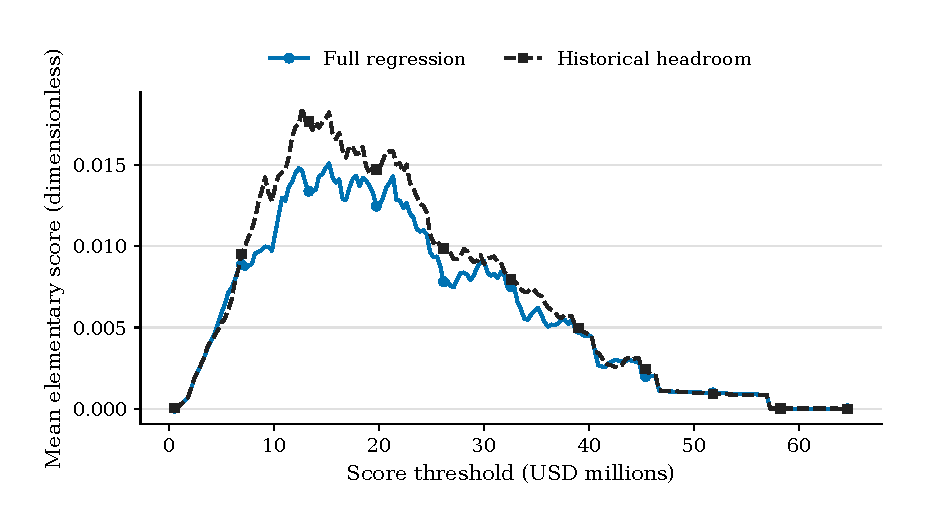
\includegraphics[width=.94\linewidth]{figures/v7-murphy-fx_hourly.pdf}
\caption{Murphy diagram for the main short-horizon FX comparison. The full-breakpoint calculation finds crossings; the graph is a display of saved scores. Average pinball superiority does not imply dominance across elementary scores.}\label{fig:murphyfx}
\end{figure}

\begin{figure}[htbp]\centering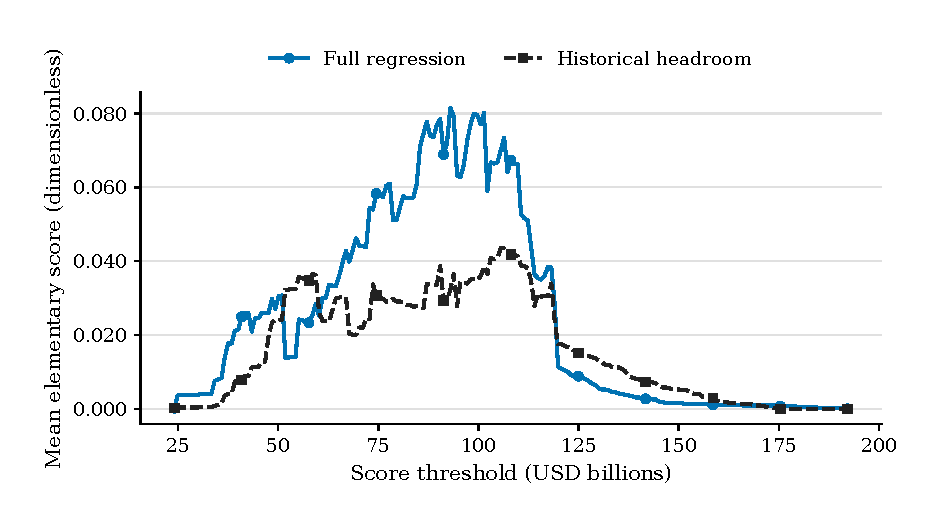
\includegraphics[width=.94\linewidth]{figures/v7-murphy-nyfed_weekly.pdf}
\caption{Murphy diagram for the main Treasury-bill comparison. The saved full-breakpoint comparison also crosses. A single average-score ordering leaves other consistent-score preferences unresolved.}\label{fig:murphybill}
\end{figure}


\section{Reproduction, availability and retained extended results}\label{sup:reproduction}

Reproduction and run records are retained verbatim in the \href{https://github.com/ByronLi0207/financial-mathematics-paper-20261020/blob/revision-v10b/notes/v10b/supplement-audit-records.md}{v10b reproduction records}.

Editable sources, aggregate results, original designs and code accompany the
paper; favorable, adverse and failed outputs remain accessible.

Document regeneration checks saved aggregates without raw observations; it
does not establish recomputed forecast accuracy or independent replication.

Code is available at \href{https://github.com/ByronLi0207/financial-mathematics-paper-20261020/tree/revision-v13}{the current repository entry}; the root \href{https://github.com/ByronLi0207/financial-mathematics-paper-20261020/blob/revision-v13/REPRODUCING.md}{reproduction instructions} identify required raw inputs and executable checks.

\paragraph{Full financial replay requires compatible inputs.}
A separately authorized replay requires the original FX member and Treasury
snapshot to match their recorded fingerprints and definitions. Restricted FX
observations and private per-origin forecasts or fitted traces are not
redistributed. Downloaded economic dates do not establish verified first-release
availability; a matching series name does not establish snapshot identity.

\paragraph{Routes to complete evidence.}
The \href{https://github.com/ByronLi0207/financial-mathematics-paper-20261020/blob/revision-v7-final/protocol/revision-v6/REPLAY.md}{v6 replay guide},
\href{https://github.com/ByronLi0207/financial-mathematics-paper-20261020/blob/revision-v7-final/results/revision-20261022/README.md}{original conditional records},
\href{https://github.com/ByronLi0207/financial-mathematics-paper-20261020/blob/revision-v7-final/results/supervisor-20261023/r6/README.md}{supervisor rule records} and
\href{https://github.com/ByronLi0207/financial-mathematics-paper-20261020/blob/revision-v7-final/EXTENDED_RESULTS.md}{extended-results index} identify the
complete retained tables, failure inventories and longer technical discussions.
Individual-dealer external validation and prospective first-release validation remain unmet.

\FloatBarrier

\section{Additional saved evidence on history length}\label{sup:v11-history}

The earlier confirmation exercise applies its fixed pooled criteria to heavy-tailed, regime-switching and compound-Poisson innovation laws. Table~\ref{tab:v11-confirmation} reports every prewritten criterion, including the failed universal ordering prediction. Its history regions use method-specific thresholds estimated in the earlier source study; they are not an oracle rule for the financial data.

\begin{table}[htbp]\centering\small
\caption{Saved confirmation criteria for excess loss relative to matched historical headroom under additional synthetic innovation laws. Counts use the original fixed pooled denominators, including all counterexamples.}\label{tab:v11-confirmation}
\begin{tabular}{p{7.2cm}rrrr}\toprule
Prewritten criterion & Successes & Missing & Required & Result \\ \midrule
Positive excess loss in the low-history region & 47/48 & 0 & 80\% & Supported \\
Negative excess loss in the high-history region & 21/24 & 0 & 60\% & Supported \\
Four-feature loss never exceeds full-regression loss & 42/48 & 0 & 100\% & Not supported \\
\bottomrule\end{tabular}
\par\smallskip\begin{minipage}{.98\linewidth}\footnotesize
History regions use the method-specific thresholds fixed in the linked original design, conditional on the earlier threshold exercise; the history index excludes predictor dimension.
Full and four-feature regressions retain different original penalty menus, so their ordering does not isolate predictor dimension.
The universal ordering prediction is not supported; the complete records retain all counterexamples and candidate failures.
\end{minipage}\end{table}


The \href{https://github.com/ByronLi0207/financial-mathematics-paper-20261020/tree/revision-v11/evidence/v11/pr5-v9}{unchanged source records} retain the complete synthetic results, counterexamples and candidate failures. The \href{https://github.com/ByronLi0207/financial-mathematics-paper-20261020/blob/revision-v11/evidence/v11/pr5-v9/protocol/revision-v9/wp2-confirmatory.md}{original confirmation design} records the fixed laws, history regions, penalty menus and decision rules. The local design commits precede their numerical runs; the later public file uploads are not public preregistration.

The complete \href{https://github.com/ByronLi0207/financial-mathematics-paper-20261020/blob/revision-v11/evidence/v11/pr5-v9/results/revision-v9/wp3/contrasts.json}{FX history contrasts} retain both horizons and every tested window. Both longer-horizon methods lose their gain again at the longest history. The four-feature short-horizon first cutpoint is left-censored and not testable, so the original confirmation across all curves is not established. These comparisons use the inspected period and provide neither evidence from an additional dealer nor a fresh financial holdout.

\section{Retained scope details and additional empirical checks}\label{sup:v12-details}

\paragraph{Earlier scope, retained verbatim.}
The following paragraphs reproduce the earlier manuscript's scope discussion verbatim. They describe the evidence available before the additional empirical checks summarized below; statements about untested work retain that historical meaning.

The FX evidence describes a single market maker's client-flow record. Its original evaluation period was viewed before the conditional methods were specified. Rules for the earlier 2015 comparison followed the original results. The full-prefix backcast uses penalties selected after its issue dates and contains the earlier backcast. Its target paths were covered by previous scoring. Both exercises remain retrospective.

The New York Fed weekly categories share a reporting system and economic components; they are related aggregate tasks, not independent dealer replications. Treasury comparisons replay the downloaded economic-date vintage. Historical publication-time information is not reconstructed. Aggregation can offset gross dealer exposure; sampled net inventory also differs from settlement cash needs. Valuation and reporting-composition changes are not separated from trading. Sampled peaks omit intervening excursions. Daily last records also differ from verified closes or intraday maxima; the source timezone and release vintage are unknown.

Daily aggregation jointly changes physical histories, horizons, update cadence, calendar predictors, evaluation span and sampled targets. The same-record comparison leaves a pure frequency effect unidentified.

The design gives no causal interpretation or individual-predictor effects. The financial procedures provide no coverage guarantee under their dependence and calibration scheme. Trading and funding gains are not measured. Scoring weights are evaluation preferences, not estimated intervention or funding costs. Independent dealer records and prospective observations would broaden validation; finer exposure and cost data would connect reports to inventory actions.

Short overlapping validation samples and research-stage selection limit tuning stability and confirmatory inference. Longer weekly outer validation windows remain untested. The simulation designs use different menus, clocks, calibration laws and summary statistics. The paired menu experiment isolates that procedure change within the calibrated laws; empirical causation remains unresolved. The new parameter-switching process repeats fitted dwell lengths and adds artificial last-to-first transitions. Its stability screen uses a plug-in model-based approximation. Moment qualification and successful optimization leave the assumed law and boundary-estimate uncertainty unresolved. Failed cells and unavailable diagnostic comparisons retain those statuses.

The statement about untested longer weekly validation windows records the earlier scope only. The additional CFTC validation-length comparison now tests longer windows on the unchanged evaluation period, with its complete outcomes and failures linked below. It does not establish prospective tuning stability.

CFTC categories provide an independent reporting system, not independent individual dealers. Full-history continuity creates a retrospective survivor universe. Open-interest ranking only orders the eligible contracts here. Conservative consolidation-family exclusions leave seventeen eligible contracts. Raw contracts have different exposure units; normalized comparisons do not recover common-dollar risks. Downloaded position dates omit actual historical first-release vintages and reporting delays. Two ingestion-schema clarifications followed acquisition but preceded every forecast and model-loss result; their original failed technical attempts remain documented.

Coefficients are fixed preferences; no estimated funding return, optimal intervention policy or trading-profit claim follows. The normalization uses evaluation-sample F headroom; ex ante institutional charges remain untested. MCS inference requires suitable loss dependence. The stationary bootstrap, modest samples and research-stage specification choices limit its nominal interpretation. Membership and cross-task fractions do not certify future coverage or simultaneous best-model status.

\paragraph{Issued-report consistency.}
Separately fitted horizon forecasts can violate the ordering of true peak quantiles. Short-history FX regression produces horizon crossings on 640 evaluation origins. Label nesting, floor coverage and strict-breach definitions provide additional checks on the issued reports.
The complete horizon-coherence comparisons remain in Section~\ref{sup:coherence}; autoregressive replay and empirical-rank details remain in Sections~\ref{sup:ar} and~\ref{sup:rank}.

\paragraph{Additional empirical checks and complete results.}
Complete source-cell records, candidate means, prewritten decisions and execution receipts are retained in \href{https://github.com/ByronLi0207/financial-mathematics-paper-20261020/tree/revision-v12/results/v12/decomposition}{the loss-decomposition results}, \href{https://github.com/ByronLi0207/financial-mathematics-paper-20261020/tree/revision-v12/results/v12/validation-length}{the validation-length results} and \href{https://github.com/ByronLi0207/financial-mathematics-paper-20261020/tree/revision-v12/results/v12/tau}{the tail-level results}. The decomposition evaluates every declared penalty on the same evaluation origins. Its best finite-penalty evaluation score is an optimistic retrospective diagnostic, not a usable selection rule. The infinite candidate is ordinary empirical headroom and is excluded from that finite oracle; the selection component may therefore be negative. Longer validation changes selection rather than evaluation dates or refit schedules. Tail-level checks change empirical ranks, fitted targets and scores together; the declared sample-maximum cap supplies no coverage guarantee. These new empirical checks require all validation candidates to complete, including for four-feature regression; the earlier simulated policy above is unchanged. Required numerical failures remain failed whole procedure cells, without retries or successful-subset substitution. Failed fits leave the highest-level CFTC threshold and two-period FX criterion unresolved; completed lower-level outputs do not replace them.

\section{Model confidence sets: retained main comparison}\label{sup:v13-mcs}

Joint comparison leaves matched historical methods alongside alternatives in most sets, with a single historical method surviving in only a small minority. These results support retaining historical controls while leaving many alternatives uneliminated under the fixed bootstrap approximation. Non-elimination does not establish equal predictive risk. Table~\ref{tab:v10-mcs-main} reports surviving methods, with identical observed-loss patterns explained separately in Supplement Section S31. Supplement Section S31 retains every set, method p-value, equivalence class and prior unavailable method.

These confidence sets use the original comparison inventory; the later validation rules are reported separately in Section~\ref{sup:v13-checks}.

\begin{table}[!htbp]\centering\footnotesize
\setlength{\tabcolsep}{4pt}
\caption{Ninety-percent model confidence sets across all planned comparisons. Counts retain their comparison or conditional-procedure denominators.}\label{tab:v10-mcs-main}
\begin{tabular}{lrrrrr}\toprule
Group & Complete & Matched history & Sole historical & Conditional & Unavailable \\
 & / planned & included & method & excluded & procedures \\ \midrule
FX original & 4/4 & \makebox[3.2em][r]{2/4} (\makebox[2.9em][r]{50.0}\%) & \makebox[3.2em][r]{0/4} (\makebox[2.9em][r]{0.0}\%) & \makebox[3.2em][r]{39/66} (\makebox[2.9em][r]{59.1}\%) & 6 \\
FX earlier period & 4/4 & \makebox[3.2em][r]{3/4} (\makebox[2.9em][r]{75.0}\%) & \makebox[3.2em][r]{0/4} (\makebox[2.9em][r]{0.0}\%) & \makebox[3.2em][r]{1/15} (\makebox[2.9em][r]{6.7}\%) & 2 \\
Treasury bills & 4/4 & \makebox[3.2em][r]{4/4} (\makebox[2.9em][r]{100.0}\%) & \makebox[3.2em][r]{0/4} (\makebox[2.9em][r]{0.0}\%) & \makebox[3.2em][r]{11/74} (\makebox[2.9em][r]{14.9}\%) & 4 \\
Other NYFed panels & 48/48 & \makebox[3.2em][r]{46/48} (\makebox[2.9em][r]{95.8}\%) & \makebox[3.2em][r]{0/48} (\makebox[2.9em][r]{0.0}\%) & \makebox[3.2em][r]{110/384} (\makebox[2.9em][r]{28.6}\%) & 48 \\
Same-record daily FX & 4/4 & \makebox[3.2em][r]{4/4} (\makebox[2.9em][r]{100.0}\%) & \makebox[3.2em][r]{2/4} (\makebox[2.9em][r]{50.0}\%) & \makebox[3.2em][r]{5/8} (\makebox[2.9em][r]{62.5}\%) & 0 \\
CFTC & 34/34 & \makebox[3.2em][r]{31/34} (\makebox[2.9em][r]{91.2}\%) & \makebox[3.2em][r]{0/34} (\makebox[2.9em][r]{0.0}\%) & \makebox[3.2em][r]{31/136} (\makebox[2.9em][r]{22.8}\%) & 0 \\
All comparisons & 98/98 & \makebox[3.2em][r]{90/98} (\makebox[2.9em][r]{91.8}\%) & \makebox[3.2em][r]{2/98} (\makebox[2.9em][r]{2.0}\%) & \makebox[3.2em][r]{197/683} (\makebox[2.9em][r]{28.8}\%) & 60 \\
\bottomrule\end{tabular}
\par\smallskip\begin{minipage}{.98\linewidth}\footnotesize
Matched history includes corrected and ordinary empirical headroom reports, excluding rolling references and nearest-neighbor baselines; conditional exclusions count complete procedures.
Identical losses can leave several methods tied, so the sole-method column counts only sets containing exactly one historical procedure.
Supplement Section S31 retains all tied loss patterns, secondary membership counts and unavailable procedures; related comparisons are not independent replications.
\end{minipage}\end{table}


\FloatBarrier
\section{Validation extensions and a retrospective decision rule}\label{sup:v13-checks}

\paragraph{Post-failure solver check.}
At the 99\% quantile, required numerical fits fail in one CFTC comparison and both FX periods. A post-failure solver repair reproduces forecasts within $10^{-6}$ pointwise relative error in only 6 of 10 previously converged fits. Unchanged residual and duality-gap thresholds reject this repair, preventing all three failed comparisons from running with the change. Their original unavailable values and both undetermined tail-level judgments remain in the \href{https://github.com/ByronLi0207/financial-mathematics-paper-20261020/tree/revision-v13/results/v13/tau-repair}{complete numerical check}, including every compatibility failure and unrun comparison.

\paragraph{Longer validation in the New York Fed series.}
Across-series median loss falls under longer validation at both horizons, extending the direction found in CFTC. Table~\ref{tab:v13-validation} reports both regression variants, including the failed short-horizon median-improvement condition for the four-feature variant. Figure~\ref{fig:v13-validation} retains every sequence beside the CFTC comparisons rather than pooling their evidence.

\begin{table}[!htbp]\centering\footnotesize\setlength{\tabcolsep}{3pt}
\caption{New York Fed validation-length comparisons on the unchanged evaluation sample. Entries are across-series median excess loss relative to corrected historical headroom, with changes in percentage points and selections of the ordinary empirical limit. Every method/horizon row contains all thirteen series.}\label{tab:v13-validation}
\begin{tabular}{lrrrrlll}\toprule
Method & $H$ & 52 weeks (\%) & 156 weeks (\%) & Change (pp) & $\infty$: 52/156 & Median screen & Shrinkage screen\\\midrule
Full regression & 6 & +6.68 & -1.13 & -7.81 & 6 / 9 & Pass & Pass \\
Full regression & 24 & +40.47 & +5.02 & -35.45 & 3 / 9 & Pass & Pass \\
Four-feature & 6 & +3.26 & -0.95 & -4.22 & 5 / 7 & Fail & Pass \\
Four-feature & 24 & +24.88 & +6.21 & -18.67 & 4 / 9 & Pass & Pass \\
\bottomrule\end{tabular}
\par\smallskip\begin{minipage}{.98\linewidth}\footnotesize The two screens are the pre-specified across-series median-improvement and increased infinite-penalty-selection conditions. Arm-median changes are not medians of paired series changes.\end{minipage}
\end{table}

The original validation origins are 329--380; longer validation uses 243--398 at the short horizon and 225--380 at the longer horizon. Evaluation remains 405--681, with 277 issues. Thus the short-horizon endpoint also advances eighteen weeks and changes the validation refit phase; this is not a causal length-only comparison. The longer-horizon endpoint is unchanged. Differences between arm medians also need not describe a typical series: for full regression, the paired-change median is +0.00 and -44.10 percentage points, respectively. All source, candidate and failure records remain in the \href{https://github.com/ByronLi0207/financial-mathematics-paper-20261020/tree/revision-v13/results/v13/nyfed-validation}{complete validation-length results}; related weekly categories are not independent dealer replications.

\begin{figure}[!htbp]\centering
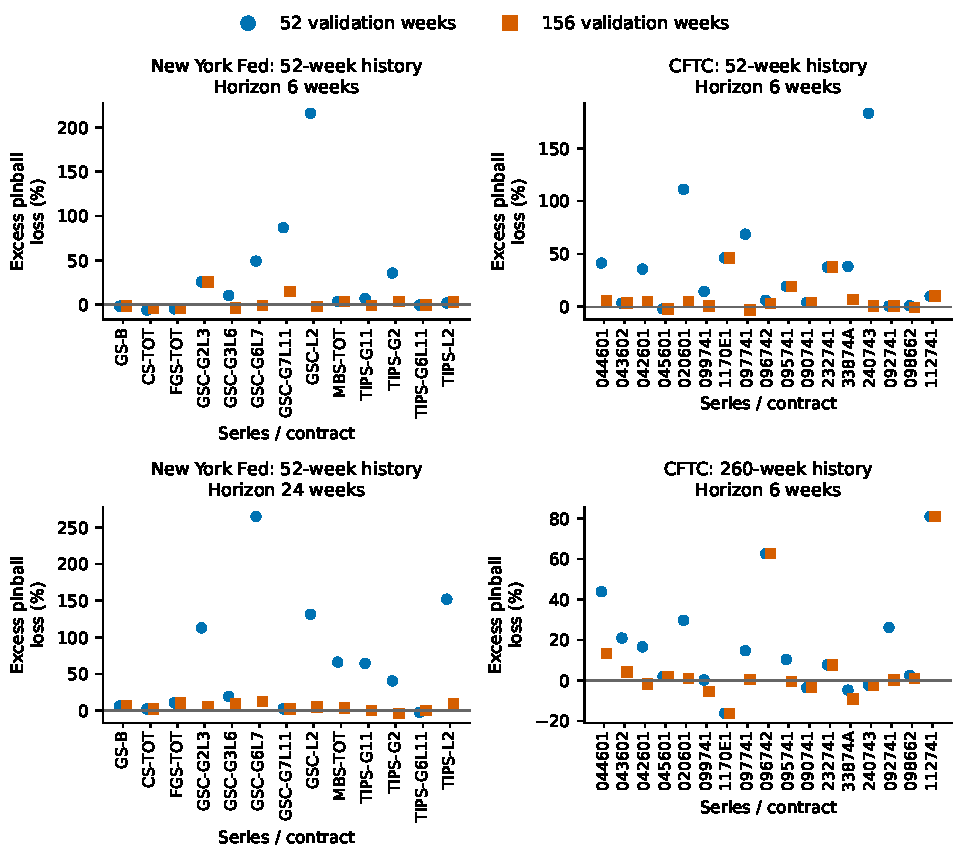
\includegraphics[width=.98\linewidth]{figures/v13-validation-length.pdf}
\caption{Full-regression losses under short and long validation samples, with each reporting system retaining its own sources and histories. Points use unchanged evaluation origins; positive excess means higher loss than matched corrected historical headroom. The New York Fed short-horizon extension also changes the endpoint and refit phase; shortened source labels omit the common PDPOS prefix, so GS-B means PDPOSGS-B.}\label{fig:v13-validation}
\end{figure}

\FloatBarrier
\paragraph{The retrospective validation protocol.}
The rule uses the six-point penalty menu, longer validation, and a historical default. Weekly validation contains 156 issues and FX validation contains 5,760; regression replaces corrected historical headroom only when its validation advantage exceeds one paired HAC standard error. Selection and the gate share validation data, and the decision stays fixed over the evaluation segment. Infinite shrinkage gives ordinary empirical headroom, so it must pass the same gate to replace the corrected-rank reference. These settings combine existing forecasting and validation methods without a nominal protection guarantee.

All 62 planned comparisons complete, including 60 weekly cells and both FX periods. The weekly median moves from +14.63\% for ordinary regression with the six-point menu to 0.00\% for the protocol. However, 8 of 60 weekly cells exceed the historical loss by more than 10\%, and the worst excess is +80.98\%. The median condition therefore passes while the tail condition fails. The protocol returns to history in 32 weekly cells and uses regression in 28, as Table~\ref{tab:v13-routing} shows. The adverse cells comprise 7 CFTC comparisons and 1 New York Fed comparison. Both FX periods retain their ordinary-regression gains, 14.77\% and 16.62\%, meeting the gain-retention condition.

\begin{table}[!htbp]\centering\footnotesize\setlength{\tabcolsep}{4pt}
\caption{Historical fallback and adverse outcomes by source, horizon and training history. Counts use every planned comparison in each row; the last column counts protocol excess loss above ten percent.}\label{tab:v13-routing}
\begin{tabular}{lrrr rr}\toprule
Source / period & $H$ & $W$ & Historical fallback & Median excess (\%) & Adverse count\\\midrule
Treasury bills & 6 & 52 & 1 / 1 & +0.00 & 0 \\
Other NY Fed series & 6 & 52 & 8 / 12 & +0.00 & 1 \\
Treasury bills & 24 & 52 & 1 / 1 & +0.00 & 0 \\
Other NY Fed series & 24 & 52 & 10 / 12 & +0.00 & 0 \\
CFTC & 6 & 52 & 6 / 17 & +0.00 & 4 \\
CFTC & 6 & 260 & 6 / 17 & +0.00 & 3 \\
FX, original & 6 & 2880 & 0 / 1 & -14.77 & 0 \\
FX, earlier & 6 & 2880 & 0 / 1 & -16.62 & 0 \\
\bottomrule\end{tabular}
\end{table}

The adverse CFTC cells are 1170E1, 095741, 232741 and 112741 at the shorter history, and 044601, 096742 and 112741 at the longer history. The remaining cell is the New York Fed two-to-three-year Treasury coupon category at the short horizon. The \href{https://github.com/ByronLi0207/financial-mathematics-paper-20261020/tree/revision-v13/results/v13/recommended-protocol}{complete protocol results} retain every comparison, selected penalty, paired gate and fallback route. The protocol was designed after inspecting earlier results, including these evaluation periods, so this is a retrospective test rather than prospective protection evidence.


\section{Audited CFTC history-length extension}\label{sup:submission-wp2}

This section imports saved results from the separately developed final-jof branch. The local design commit precedes calculation; public upload occurred after calculation. This is not an externally registered or prospective financial confirmation.

The shorter-history outcomes had already been inspected. Only the longest-history forecasts were added under the fixed extension design. The same downloaded CFTC source arrays and reporting-vintage limitations apply.

\begin{table}[htbp]\centering\small

\caption{Fixed history-length decision screens, including failed and untestable predictions. Counts use the original planned denominators.}\label{tab:submission-wp2}

\begin{tabular}{lllll}\toprule

Screen & Regression & Successes / planned & Required fraction & Judgment\\\midrule

P1 & Four-feature & 15 / 17 & 80\% & Supported\\

P1 & Full & 29 / 34 & 80\% & Supported\\

P2 & Four-feature & 10 / 17 & 60\% & Not supported\\

P2 & Full & --- & --- & Not testable\\

P3 & Four-feature & 6 / 17 & 70\% & Not supported\\

\bottomrule\end{tabular}\end{table}

Both low-history disadvantage screens pass. The longer-history advantage screen and strict sequential-improvement screen fail. The full regression has no prewritten high-region cell. The retained overall judgment is partial support.

\paragraph{Complete counterexample inventory.} The following rows retain every saved counterexample. A market can appear under several screens. Loss changes are relative to the matched historical reference; their signs do not redefine a screen after observing it.

\begin{longtable}{lllp{7.5cm}}

\caption{All saved counterexamples to the transported history screens.}\label{tab:submission-wp2-counterexamples}\\

\toprule Screen & Market code & History & Relative loss change (percent)\\\midrule\endfirsthead

\toprule Screen & Market code & History & Relative loss change (percent)\\\midrule\endhead

P1\_QR4 & 240743 & 52 & -7.324391\\

P1\_QR4 & 098662 & 52 & -0.437432\\

P2\_QR4 & 044601 & 520 & +0.811445\\

P2\_QR4 & 043602 & 520 & +8.026475\\

P2\_QR4 & 042601 & 520 & +1.137518\\

P2\_QR4 & 045601 & 520 & +1.520938\\

P2\_QR4 & 099741 & 520 & +0.618103\\

P2\_QR4 & 095741 & 520 & +3.875925\\

P2\_QR4 & 232741 & 520 & +0.575901\\

P1\_QR33 & 045601 & 52 & -2.041454\\

P1\_QR33 & 1170E1 & 260 & -16.215517\\

P1\_QR33 & 090741 & 260 & -3.599484\\

P1\_QR33 & 33874A & 260 & -4.775476\\

P1\_QR33 & 240743 & 260 & -2.283380\\

P3\_QR4 & 042601 & 52/260/520 & +9.475655, +74.230130, +1.137518\\

P3\_QR4 & 045601 & 52/260/520 & +0.311844, +1.845046, +1.520938\\

P3\_QR4 & 099741 & 52/260/520 & +13.973619, +0.217492, +0.618103\\

P3\_QR4 & 1170E1 & 52/260/520 & +6.823794, -28.436244, -25.194932\\

P3\_QR4 & 097741 & 52/260/520 & +23.757442, -6.540749, -4.288684\\

P3\_QR4 & 096742 & 52/260/520 & +3.411816, +4.815826, -17.900542\\

P3\_QR4 & 095741 & 52/260/520 & +19.545430, +2.130022, +3.875925\\

P3\_QR4 & 090741 & 52/260/520 & +10.280676, -5.346398, -0.963088\\

P3\_QR4 & 232741 & 52/260/520 & +123.325833, -3.354286, +0.575901\\

P3\_QR4 & 240743 & 52/260/520 & -7.324391, -2.283380, -7.696425\\

P3\_QR4 & 098662 & 52/260/520 & -0.437432, -39.440706, -0.546595\\

\bottomrule\end{longtable}

\paragraph{Provenance and interpretation.} The design was committed locally before the recorded execution start; the audit records both original commit identities and their UTC times. The saved summary retains its execution-stage verification marker; later acceptance and scalar-check receipts supply the completed audit status. Scalar agreement by the same executor is not independent dealer replication or another solver fit.

Full cells, candidate reports, execution receipts and source identities are preserved in \href{https://github.com/ByronLi0207/financial-mathematics-paper-20261020/tree/submission-final/evidence/submission/final-jof/results/final-merge/wp2-cftc-mechanism}{the audited result archive}. The \href{https://github.com/ByronLi0207/financial-mathematics-paper-20261020/blob/submission-final/notes/submission/import-audit.md}{import audit} distinguishes original data from additional non-data code dependencies. These related-market counts establish neither a sufficient financial history nor a causal mechanism.

% Generated by notes/submission/generate_prediction_table.py; do not hand edit.
% Register SHA256: c4e51ec51c0b15653726cabaf02d45130e919295a0f0127aead359af4bda3987
\clearpage
\section{Prewritten predictions, thresholds and saved judgments}\label{sup:submission-predictions}
This register prints every saved prediction without fitting models, recomputing thresholds or changing a saved judgment. Round gives the complete row identifier and its recorded role. Supported, Not supported and Undetermined translate the saved decision only; saved status strings and unavailable reasons remain explicit.
Prewritten before the indicated new calculations does not imply original-study preregistration, an untouched evaluation period or external-registry preregistration. Public Git posting and local pre-run designs are distinct. E5 has only a saved receipt for its local pre-run design: the original design Git object is unavailable, and its public file upload followed the recorded run. R6, E1, E2 and WP2 have verified local pre-run designs but public file uploads after calculation. F1, F2, F3, G2 and G3 have local and public Git design commits before their new calculations; their inspected-study and retrospective limits still apply.
Panel A retains the primary and secondary rows. Panel B separately retains all QR4 sensitivity rows; they cannot replace a primary QR33 judgment. This separation does not relabel the originally primary QR4 predictions in E2 or WP2. Related series and markets do not create independent dealer replications.
WP2 adds only W520 forecasts; W52/W260 outcomes were already known. Its QR33 high-region row remains structurally NOT\_TESTABLE with planned=0 and NO\_REGISTERED\_REGION\_CELL. Both low-region methods support combined P1, but the saved overall primary verdict remains PARTLY; the secondary P3 cannot upgrade it.
\begingroup
\fontsize{8.5}{10.2}\selectfont
\setlength{\tabcolsep}{2pt}
\renewcommand{\arraystretch}{1.12}
\setlength{\LTcapwidth}{\linewidth}
\begin{longtable}{@{}>{\raggedright\arraybackslash}p{18mm}>{\raggedright\arraybackslash}p{33mm}>{\raggedright\arraybackslash}p{30mm}>{\raggedright\arraybackslash}p{43mm}>{\raggedright\arraybackslash}p{20mm}>{\raggedright\arraybackslash}p{17mm}@{}}
\caption{All saved prewritten prediction rows. Thresholds, results and judgments are copied from the bound register; numeric precision is retained.}\label{tab:submission-predictions}\\
\toprule Round & Prediction & Threshold & Saved result & Judgment & Location \\\midrule
\endfirsthead
\caption[]{Continued.}\\
\toprule Round & Prediction & Threshold & Saved result & Judgment & Location \\\midrule
\endhead
\midrule\multicolumn{6}{r}{\emph{Continued on next page}}\\
\endfoot
\bottomrule\endlastfoot
\multicolumn{6}{@{}l}{\textbf{Panel A. Primary and secondary predictions}}\\*\midrule
% row_id: E5.P1.QR33+
\texttt{E5.\allowbreak{}P1.\allowbreak{}QR33+}\par primary & QR33+ strictly improves original QR33 loss within the 45 originally adverse panel cells. & At least 40 of fixed 45 cells. & 30/\allowbreak{}45 successes; required 40. & Not supported\par\texttt{false} & Supplement\par Sections\par \ref{sup:panel}, \ref{sup:panel-second};\par Main Table 5 \\[3pt]
% row_id: E5.P2.QR33+
\texttt{E5.\allowbreak{}P2.\allowbreak{}QR33+}\par primary & QR33+ excess loss against F lies within inclusive [-10\%,\allowbreak{} +10\%]. & At least 36 of fixed 48 cells within [-10,\allowbreak{} +10]\%. & 24/\allowbreak{}48 successes; required 36. & Not supported\par\texttt{false} & Supplement\par Sections\par \ref{sup:panel}, \ref{sup:panel-second};\par Main Table 5 \\[3pt]
% row_id: E5.P3.QR33+
\texttt{E5.\allowbreak{}P3.\allowbreak{}QR33+}\par primary & Selected ridge penalty is at least 1. & At least 25 of fixed 48 cells (more than half). & 33/\allowbreak{}48 successes; required 25. & Supported\par\texttt{true} & Supplement\par Sections\par \ref{sup:panel}, \ref{sup:panel-second};\par Main Table 5 \\[3pt]
% row_id: R6.S1.R2
\texttt{R6.\allowbreak{}S1.\allowbreak{}R2}\par primary & All 26 retrospective weekly R2 cells complete with bounded worst and median excess. & 26/\allowbreak{}26 complete; worst \ensuremath{<}=\allowbreak{} +25\%; median \ensuremath{<}=\allowbreak{} +5\%. & 26/\allowbreak{}26 complete; worst 181.39452368014167\%; median 5.374072481175762\%. & Not supported\par\texttt{NOT\_\allowbreak{}MET} & Supplement\par Sections\par \ref{sup:selection}, \ref{sup:selection-failures};\par Main Table 5 \\[3pt]
% row_id: R6.S2.R2
\texttt{R6.\allowbreak{}S2.\allowbreak{}R2}\par primary & R2 retains at least half of each negative R0 FX H6 gain. & For each eligible R0 \ensuremath{<} 0 cell,\allowbreak{} R2 \ensuremath{<}=\allowbreak{} 0.5*R0; at least one eligible cell required. & One eligible cell W2880: R0 =\allowbreak{} -16.62356533682211\%; R2 =\allowbreak{} -6.2754532709491055\%; half\_\allowbreak{}gain\_\allowbreak{}retained =\allowbreak{} false. W720 not eligible. & Not supported\par\texttt{NOT\_\allowbreak{}MET} & Supplement\par Sections\par \ref{sup:selection}, \ref{sup:selection-failures};\par Main Table 5 \\[3pt]
% row_id: R6.S3.R2
\texttt{R6.\allowbreak{}S3.\allowbreak{}R2}\par primary & R2 weekly median excess is strictly lower than R0. & Both rules complete 26 cells; median(R2) \ensuremath{<} median(R0). & R0 median 4.1510024714803695\%; R2 median 5.374072481175762\%; both 26 complete. & Not supported\par\texttt{NOT\_\allowbreak{}MET} & Supplement\par Sections\par \ref{sup:selection}, \ref{sup:selection-failures};\par Main Table 5 \\[3pt]
% row_id: E1.M1.QR33
\texttt{E1.\allowbreak{}M1.\allowbreak{}QR33}\par primary & Constant-arm W52 QR33 median is near parity with F. & Inclusive [-5,\allowbreak{} +5]\%. & 0.2069371499562489\%. & Supported\par\texttt{SUPPORTED} & Supplement Section~\ref{sup:v10-menu} \\[3pt]
% row_id: E1.M2.QR33
\texttt{E1.\allowbreak{}M2.\allowbreak{}QR33}\par primary & Switching-arm W52 QR33 median exceeds constant-arm median by 5 pp. & Switching minus constant \ensuremath{>}=\allowbreak{} +5 pp. & -0.43471629487539243 pp; constant 0.2069371499562489\%; switching -0.22777914491914353\%. & Not supported\par\texttt{NOT\_\allowbreak{}SUPPORTED} & Supplement Section~\ref{sup:v10-menu} \\[3pt]
% row_id: E1.M3.QR33
\texttt{E1.\allowbreak{}M3.\allowbreak{}QR33}\par primary & Both arm medians improve and at least 12 of 13 sources improve in both arms. & Both group arm medians strictly lower; joint improvement \ensuremath{>}=\allowbreak{} 12/\allowbreak{}13. & Both group arms improve; joint\_\allowbreak{}improved\_\allowbreak{}sources =\allowbreak{} 13/\allowbreak{}13. & Supported\par\texttt{SUPPORTED} & Supplement Section~\ref{sup:v10-menu} \\[3pt]
% row_id: E2.T1.QR33
\texttt{E2.\allowbreak{}T1.\allowbreak{}QR33}\par primary & Realized better historical report min(F,\allowbreak{} I) strictly beats QR33. & At least 60\% of all 2K cells; no missing operand deletion. & 29/\allowbreak{}34; fraction 0.8529411764705882. & Supported\par\texttt{SUPPORTED} & Supplement Section~\ref{sup:v10-cftc};\par Main Table 6 \\[3pt]
% row_id: E2.T2.QR33
\texttt{E2.\allowbreak{}T2.\allowbreak{}QR33}\par primary & Each W QR33 median excess against F lies near parity. & Inclusive [-10,\allowbreak{} +10]\% at both W52 and W260. & W52 =\allowbreak{} 19.334715757564624\%; W260 =\allowbreak{} 10.34828178946443\%. & Not supported\par\texttt{NOT\_\allowbreak{}SUPPORTED} & Supplement Section~\ref{sup:v10-cftc};\par Main Table 6 \\[3pt]
% row_id: E2.T3.QR4
\texttt{E2.\allowbreak{}T3.\allowbreak{}QR4}\par primary & QR4 median excess is strictly lower with W260 than W52. & W260 median \ensuremath{<} W52 median. & W52 =\allowbreak{} 10.280676300222424\%; W260 =\allowbreak{} 0.2174917571722501\%; change =\allowbreak{} -10.063184543050173 pp. & Supported\par\texttt{SUPPORTED} & Supplement Section~\ref{sup:v10-cftc};\par Main Table 6 \\[3pt]
% row_id: F1.D1.QR33
\texttt{F1.\allowbreak{}D1.\allowbreak{}QR33}\par primary & Strictly positive finite-menu oracle gap G in more than half of fixed 41 short-weekly cells. & Fixed 41 denominator; positive G share \ensuremath{>} 1/\allowbreak{}2,\allowbreak{} using missing bounds. & support =\allowbreak{} 29/\allowbreak{}41; complete =\allowbreak{} 41; unavailable =\allowbreak{} 0; bounds =\allowbreak{} 0.7073170731707317,\allowbreak{} 0.7073170731707317. & Supported\par\texttt{SUPPORTED} & Supplement Section~\ref{sup:v12-details} \\[3pt]
% row_id: F1.D2.QR33
\texttt{F1.\allowbreak{}D2.\allowbreak{}QR33}\par primary & Positive actual excess E and selection component S \ensuremath{>} E/\allowbreak{}2 in more than half of fixed 41 cells. & Fixed 41 denominator; share of E \ensuremath{>} 0 and S \ensuremath{>} E/\allowbreak{}2 \ensuremath{>} 1/\allowbreak{}2,\allowbreak{} using missing bounds. & support =\allowbreak{} 27/\allowbreak{}41; complete =\allowbreak{} 41; unavailable =\allowbreak{} 0; bounds =\allowbreak{} 0.6585365853658537,\allowbreak{} 0.6585365853658537. & Supported\par\texttt{SUPPORTED} & Supplement Section~\ref{sup:v12-details} \\[3pt]
% row_id: F1.D3.QR33
\texttt{F1.\allowbreak{}D3.\allowbreak{}QR33}\par primary & Both original long-history FX horizons have negative finite-menu gap. & G \ensuremath{<} 0 at H6 and H24; conjunction of both original FX cells. & H6 G =\allowbreak{} -14.917351765503492\%; H24 G =\allowbreak{} -3.7577697957958254\%; 2/\allowbreak{}2 support. & Supported\par\texttt{SUPPORTED} & Supplement Section~\ref{sup:v12-details} \\[3pt]
% row_id: F2.V1.QR33
\texttt{F2.\allowbreak{}V1.\allowbreak{}QR33}\par primary & Longer CFTC validation reduces each W across-contract QR33 arm median by at least 5 pp. & For each W52/\allowbreak{}W260: median(V156)-median(V52) \ensuremath{<}=\allowbreak{} -5 pp; both required. & W52: delta =\allowbreak{} -15.304032374564795 pp,\allowbreak{} pairs =\allowbreak{} 17/\allowbreak{}17,\allowbreak{} missing =\allowbreak{} 0; W260: delta =\allowbreak{} -9.82319311344436 pp,\allowbreak{} pairs =\allowbreak{} 17/\allowbreak{}17,\allowbreak{} missing =\allowbreak{} 0. & Supported\par\texttt{SUPPORTED} & Supplement\par Sections\par \ref{sup:v12-details}, \ref{sup:v13-checks};\par Main Table 7 \\[3pt]
% row_id: F2.V2.QR33
\texttt{F2.\allowbreak{}V2.\allowbreak{}QR33}\par primary & Longer CFTC validation raises empirical-limit selection frequency at each W. & At each W52/\allowbreak{}W260: infinity count(V156) \ensuremath{>} count(V52); both required. & W52: infinity V52/\allowbreak{}V156 =\allowbreak{} 4/\allowbreak{}10,\allowbreak{} missing\_\allowbreak{}pairs =\allowbreak{} 0; W260: infinity V52/\allowbreak{}V156 =\allowbreak{} 4/\allowbreak{}5,\allowbreak{} missing\_\allowbreak{}pairs =\allowbreak{} 0. & Supported\par\texttt{SUPPORTED} & Supplement\par Sections\par \ref{sup:v12-details}, \ref{sup:v13-checks};\par Main Table 7 \\[3pt]
% row_id: F3.Q1.QR33
\texttt{F3.\allowbreak{}Q1.\allowbreak{}QR33}\par primary & At tau .99 F strictly beats QR33 in at least 29 fixed CFTC cells. & At least 29/\allowbreak{}34; strict wins only; fixed denominator with unknown bounds. & 28 supports,\allowbreak{} 5 complete nonsupports (4 exact ties),\allowbreak{} 1 unknown; support bounds [0.8235294117647058,\allowbreak{} 0.8529411764705882]. & Undetermined\par\texttt{UNDETERMINED} & Supplement Section~\ref{sup:v13-checks};\par Main Table 8 \\[3pt]
% row_id: F3.Q2.QR33
\texttt{F3.\allowbreak{}Q2.\allowbreak{}QR33}\par primary & At tau .99 QR33 improves matched F in both FX periods. & Relative excess \ensuremath{<} 0 in original and early 2015; both required. & Both period inputs FAILED; 0 supports,\allowbreak{} 2 unknown; both relative\_\allowbreak{}loss\_\allowbreak{}pct =\allowbreak{} null. & Undetermined\par\texttt{UNDETERMINED} & Supplement Section~\ref{sup:v13-checks};\par Main Table 8 \\[3pt]
% row_id: G2.V3.QR33
\texttt{G2.\allowbreak{}V3.\allowbreak{}QR33}\par primary & Longer NY Fed validation reduces each horizon across 13 arm median by at least 5 pp. & At each H6/\allowbreak{}H24: median(V156)-median(V52) \ensuremath{<}=\allowbreak{} -5 pp; both required. & H6: -7.812971755453957 pp (SUPPORTED); H24: -35.45092255436495 pp (SUPPORTED). & Supported\par\texttt{SUPPORTED} & Supplement Section~\ref{sup:v13-checks};\par Main Table 7 \\[3pt]
% row_id: G2.V4.QR33
\texttt{G2.\allowbreak{}V4.\allowbreak{}QR33}\par primary & Longer NY Fed validation increases empirical-limit selections at each horizon. & At each H6/\allowbreak{}H24: infinity count(V156) \ensuremath{>} count(V52); both required. & H6: 6 to 9 (SUPPORTED); H24: 3 to 9 (SUPPORTED). & Supported\par\texttt{SUPPORTED} & Supplement Section~\ref{sup:v13-checks};\par Main Table 7 \\[3pt]
% row_id: G3.R1.RP
\texttt{G3.\allowbreak{}R1.\allowbreak{}RP}\par primary & Protocol median excess is small across all 60 eligible weekly cells. & Full-universe median \ensuremath{<}=\allowbreak{} +1\%; any eligible missing outcome =\allowbreak{}\ensuremath{>} UNDETERMINED. & All 60 complete; median 0.0\%; ordinary-regression median 14.627467605779144\%. & Supported\par\texttt{SUPPORTED} & Supplement Section~\ref{sup:v13-checks} \\[3pt]
% row_id: G3.R2.RP
\texttt{G3.\allowbreak{}R2.\allowbreak{}RP}\par primary & At most 5\% of eligible weekly cells lose more than 10\% against F. & Adverse defined excess \ensuremath{>} 10\%; adverse fraction \ensuremath{<}=\allowbreak{} 0.05; at most 3 of 60. & 8/\allowbreak{}60 adverse; worst 80.98396986931891\%; no unavailable cells. & Not supported\par\texttt{NOT\_\allowbreak{}SUPPORTED} & Supplement Section~\ref{sup:v13-checks} \\[3pt]
% row_id: G3.R3.RP
\texttt{G3.\allowbreak{}R3.\allowbreak{}RP}\par primary & Retain at least half of ordinary QR gain in every eligible FX period. & If ordinary excess \ensuremath{<} 0,\allowbreak{} RP excess \ensuremath{<}=\allowbreak{} 0.5*ordinary; every eligible gain period and at least 1 required. & Original ordinary/\allowbreak{}RP =\allowbreak{} -14.766762552613882\% (threshold -7.383381276306941\%); early 2015 ordinary/\allowbreak{}RP =\allowbreak{} -16.623565336822104\% (threshold -8.311782668411052\%); both SUPPORTED. & Supported\par\texttt{SUPPORTED} & Supplement Section~\ref{sup:v13-checks} \\[3pt]
% row_id: WP2.P1_QR4.QR4
\texttt{WP2.\allowbreak{}P1\_\allowbreak{}QR4.\allowbreak{}QR4}\par primary & Low-region QR4 strictly loses against matched F. & At least 80\% of fixed 17 low-region cells; combined P1 requires both methods. & 15/\allowbreak{}17; 0.8823529411764706; SUPPORT. & Supported\par\texttt{SUPPORT} & Supplement Section~\ref{sup:submission-wp2} \\[3pt]
% row_id: WP2.P1_QR33.QR33
\texttt{WP2.\allowbreak{}P1\_\allowbreak{}QR33.\allowbreak{}QR33}\par primary & Low-region QR33 strictly loses against matched F. & At least 80\% of fixed 34 low-region cells; combined P1 requires both methods. & 29/\allowbreak{}34; 0.8529411764705882; SUPPORT. & Supported\par\texttt{SUPPORT} & Supplement Section~\ref{sup:submission-wp2} \\[3pt]
% row_id: WP2.P2_QR4.QR4
\texttt{WP2.\allowbreak{}P2\_\allowbreak{}QR4.\allowbreak{}QR4}\par primary & High-region W520 QR4 strictly beats matched F. & At least 60\% of fixed 17 high-region cells. & 10/\allowbreak{}17; 0.5882352941176471 below 0.6; NOT\_\allowbreak{}SUPPORT. & Not supported\par\texttt{NOT\_\allowbreak{}SUPPORT} & Supplement Section~\ref{sup:submission-wp2} \\[3pt]
% row_id: WP2.P2_QR33.QR33
\texttt{WP2.\allowbreak{}P2\_\allowbreak{}QR33.\allowbreak{}QR33}\par primary & QR33 high-region comparison requires observed c \ensuremath{>} 2 r*. & No registered high-region cell exists; structurally NOT\_\allowbreak{}TESTABLE by design. & planned =\allowbreak{} 0; NO\_\allowbreak{}REGISTERED\_\allowbreak{}REGION\_\allowbreak{}CELL; NOT\_\allowbreak{}TESTABLE. & Undetermined\par\texttt{NOT\_\allowbreak{}TESTABLE} & Supplement Section~\ref{sup:submission-wp2} \\[3pt]
% row_id: WP2.P3_QR4.QR4
\texttt{WP2.\allowbreak{}P3\_\allowbreak{}QR4.\allowbreak{}QR4}\par secondary & QR4 excess loss strictly decreases at both successive history steps. & At least 70\% of fixed 17 markets satisfy Delta 52 \ensuremath{>} Delta 260 \ensuremath{>} Delta 520. & 6/\allowbreak{}17; 0.35294117647058826 below 0.7; NOT\_\allowbreak{}SUPPORT. & Not supported\par\texttt{NOT\_\allowbreak{}SUPPORT} & Supplement Section~\ref{sup:submission-wp2} \\[3pt]
\multicolumn{6}{@{}l}{\textbf{Panel B. Separate QR4 sensitivity predictions}}\\*\midrule
% row_id: F1.D1.QR4
\texttt{F1.\allowbreak{}D1.\allowbreak{}QR4}\par sensitivity & Strictly positive finite-menu oracle gap G in more than half of fixed 41 short-weekly cells. & Fixed 41 denominator; positive G share \ensuremath{>} 1/\allowbreak{}2,\allowbreak{} using missing bounds. & support =\allowbreak{} 26/\allowbreak{}41; complete =\allowbreak{} 39; unavailable =\allowbreak{} 2; bounds =\allowbreak{} 0.6341463414634146,\allowbreak{} 0.6829268292682927. & Supported\par\texttt{SUPPORTED} & Supplement Section~\ref{sup:v12-details} \\[3pt]
% row_id: F1.D2.QR4
\texttt{F1.\allowbreak{}D2.\allowbreak{}QR4}\par sensitivity & Positive actual excess E and selection component S \ensuremath{>} E/\allowbreak{}2 in more than half of fixed 41 cells. & Fixed 41 denominator; share of E \ensuremath{>} 0 and S \ensuremath{>} E/\allowbreak{}2 \ensuremath{>} 1/\allowbreak{}2,\allowbreak{} using missing bounds. & support =\allowbreak{} 27/\allowbreak{}41; complete =\allowbreak{} 39; unavailable =\allowbreak{} 2; bounds =\allowbreak{} 0.6585365853658537,\allowbreak{} 0.7073170731707317. & Supported\par\texttt{SUPPORTED} & Supplement Section~\ref{sup:v12-details} \\[3pt]
% row_id: F1.D3.QR4
\texttt{F1.\allowbreak{}D3.\allowbreak{}QR4}\par sensitivity & Both original long-history FX horizons have negative finite-menu gap. & G \ensuremath{<} 0 at H6 and H24; conjunction of both original FX cells. & H6 G =\allowbreak{} -4.2893706508927965\%; H24 G =\allowbreak{} -3.1505838975205966\%; 2/\allowbreak{}2 support. & Supported\par\texttt{SUPPORTED} & Supplement Section~\ref{sup:v12-details} \\[3pt]
% row_id: F2.V1.QR4
\texttt{F2.\allowbreak{}V1.\allowbreak{}QR4}\par sensitivity & Longer CFTC validation reduces each W across-contract QR4 arm median by at least 5 pp. & For each W52/\allowbreak{}W260: median(V156)-median(V52) \ensuremath{<}=\allowbreak{} -5 pp; both required. & W52: delta =\allowbreak{} None pp,\allowbreak{} pairs =\allowbreak{} 16/\allowbreak{}17,\allowbreak{} missing =\allowbreak{} 1; W260: delta =\allowbreak{} None pp,\allowbreak{} pairs =\allowbreak{} 16/\allowbreak{}17,\allowbreak{} missing =\allowbreak{} 1. & Undetermined\par\texttt{UNDETERMINED} & Supplement\par Sections\par \ref{sup:v12-details}, \ref{sup:v13-checks};\par Main Table 7 \\[3pt]
% row_id: F2.V2.QR4
\texttt{F2.\allowbreak{}V2.\allowbreak{}QR4}\par sensitivity & Longer CFTC validation raises empirical-limit selection frequency at each W. & At each W52/\allowbreak{}W260: infinity count(V156) \ensuremath{>} count(V52); both required. & W52: infinity V52/\allowbreak{}V156 =\allowbreak{} 2/\allowbreak{}7,\allowbreak{} missing\_\allowbreak{}pairs =\allowbreak{} 1; W260: infinity V52/\allowbreak{}V156 =\allowbreak{} 2/\allowbreak{}4,\allowbreak{} missing\_\allowbreak{}pairs =\allowbreak{} 1. & Undetermined\par\texttt{UNDETERMINED} & Supplement\par Sections\par \ref{sup:v12-details}, \ref{sup:v13-checks};\par Main Table 7 \\[3pt]
% row_id: G2.V3.QR4
\texttt{G2.\allowbreak{}V3.\allowbreak{}QR4}\par sensitivity & Longer NY Fed validation reduces each horizon across 13 arm median by at least 5 pp. & At each H6/\allowbreak{}H24: median(V156)-median(V52) \ensuremath{<}=\allowbreak{} -5 pp; both required. & H6: -4.2150390061995235 pp (NOT\_\allowbreak{}SUPPORTED); H24: -18.670087236167987 pp (SUPPORTED). & Not supported\par\texttt{NOT\_\allowbreak{}SUPPORTED} & Supplement Section~\ref{sup:v13-checks};\par Main Table 7 \\[3pt]
% row_id: G2.V4.QR4
\texttt{G2.\allowbreak{}V4.\allowbreak{}QR4}\par sensitivity & Longer NY Fed validation increases empirical-limit selections at each horizon. & At each H6/\allowbreak{}H24: infinity count(V156) \ensuremath{>} count(V52); both required. & H6: 5 to 7 (SUPPORTED); H24: 4 to 9 (SUPPORTED). & Supported\par\texttt{SUPPORTED} & Supplement Section~\ref{sup:v13-checks};\par Main Table 7 \\[3pt]
\end{longtable}
\endgroup
The display-bindings JSON retains raw fields, JSON Pointers and SHA256 values.


\FloatBarrier
% Self-contained bibliography for supporting methods.
\nocite{*}
\input{supplement.bbl}
\end{document}
